\documentclass[11pt,a4paper]{article}
\usepackage[margin=25mm]{geometry}
\usepackage[T1]{fontenc}
\usepackage[utf8]{inputenc}
\usepackage{lmodern}
\usepackage{microtype}
\usepackage{parskip}
\setlength{\parindent}{0pt}
\widowpenalty=10000
\clubpenalty=10000
\renewenvironment{abstract}{\small\begin{center}\bfseries\abstractname\end{center}\begin{quote}\setlength{\parindent}{0pt}\setlength{\parskip}{4pt}}{\end{quote}}
\usepackage{amsmath,amssymb,amsthm,mathtools}
\usepackage{booktabs,tabularx,array}
\usepackage{graphicx,float}
\usepackage{xcolor}
\usepackage{enumitem}
\usepackage{hyperref}
\usepackage{url}
\usepackage[numbers,sort&compress]{natbib}
\urlstyle{same}
\usepackage{fancyhdr}
\usepackage{placeins}
\hypersetup{colorlinks=true,linkcolor=blue!45!black,citecolor=blue!45!black,urlcolor=blue!45!black,pdftitle={Gabriel: Contractive Dynamics, Temporal Memory and Selective Observation},pdfauthor={Sebastian Klemm}}
\setlist{topsep=4pt,itemsep=2pt,parsep=0pt}
\pagestyle{fancy}\fancyhf{}\fancyhead[L]{\small Gabriel}\fancyhead[R]{\small Dynamics, memory and decisions}\fancyfoot[C]{\thepage}
\setlength{\headheight}{14pt}
\renewcommand{\topfraction}{0.9}
\renewcommand{\textfraction}{0.07}
\renewcommand{\floatpagefraction}{0.85}
\newtheorem{theorem}{Theorem}[section]
\newtheorem{proposition}[theorem]{Proposition}
\newtheorem{corollary}[theorem]{Corollary}
\theoremstyle{definition}\newtheorem{definition}[theorem]{Definition}
\newcommand{\R}{\mathbb{R}}
\newcommand{\norm}[1]{\left\lVert#1\right\rVert}
\newcommand{\soft}{\mathcal{S}}
\newcommand{\state}{\mathcal{X}}
\title{\textbf{Gabriel}\\[4pt]\Large Contractive Dynamics, Temporal Memory\\and Selective Observation}
\author{Sebastian Klemm}
\date{27 September 2026}
\begin{document}
\maketitle
\begin{abstract}
We develop an executable architecture for controlled recurrent dynamics, temporal memory and decisions from incomplete observations. A gain budget contracts the complete activity--trace state despite changing support. Event and elapsed-time memories have explicit update and refinement contracts. Conditional output bounds distinguish unresolved model decisions from numerical conservatism; four external datasets expose task-dependent prediction--retrieval tradeoffs. Sign-transported traces preserve contraction, while finite-history and error-budget interfaces certify targets over compatible records. On a 12-cell annular model with one persistent report error, an adaptive policy uses 12--17 of 24 coordinates, matching an EC$^2$ control on 102400 cases.

A financial specialization joins convex-mixture CVaR, rational risk witnesses and acceptable-action regions. Budgeted planning lowers mean acquisition cost without increasing its worst-case bound. An immutable issue ledger connects forecasts to delayed and corrected outcomes. Frequency and severity feedback admit explicit accounting, while convex aggregation in reciprocal-risk coordinates provides an exact per-outcome comparison and maturity-ordered regret bound. External reference-rate experiments retain both positive and negative results: a fixed two-scale filter improves raw historical simulation on eight 2020--2025 targets, but a fast filter is better on six; frequency feedback worsens all eight subsequent joint scores. An adaptive pool improves uniform arithmetic pooling on seven of eight additional asset contracts but fails its prespecified comparison against all controls. Gradient-memory refinement likewise fails the combined selection conditions.

A transactional runtime composes these modules with replayable evidence and preserved issued outputs. Incremental evaluation, exact graph-orbit lookup and guarded spectral reuse reduce specific execution costs under separate preservation contracts. A native graph observer specializes recognized weighted cliques through two projectors; its fixed-region responses have at most three temporal components. Complete 256-query native tasks improve by factors 2.03--3.11, while process, identity and storage costs largely absorb that advantage at the owner boundary.

A separate exact-input extension uses Arb enclosures to certify regional threshold crossings over continuous time windows. Analytic and validated adaptive methods resolve all 256 primary cases identically; the prespecified timing-superiority criterion fails. The integrated owner executes 96 checked window answers in 24 complete tasks. Persistence controls identify storage-environment limits without explaining historical prefix regressions. The result is a reproducible family of conditional guarantees and measured task comparisons, not a demonstration of general predictive or platform superiority.
\end{abstract}
{\small\textbf{Keywords:} recurrent networks; contraction; temporal memory; partial observation; decision regions; active feature acquisition; robust risk; exact certificates.}
\newpage
\begingroup
\footnotesize
\setcounter{tocdepth}{1}
\setlength{\parskip}{0pt}
\tableofcontents
\endgroup
\newpage

\section{Computational question and relation to prior work}
Gabriel is a modular computational architecture for temporal representation and decisions under partial observation. Its local recurrent units are Gabriel cells. The organizing question is which properties can be guaranteed about evolving state, retained information and justified actions when the domain model and available evidence are explicit. A shared transactional owner supplies an executable composition boundary for finite observation and maturity feedback; Section~\ref{sec:runtime} specifies which component behaviors it preserves. Section~\ref{sec:stream} closes an observation-to-forecast loop while retaining immutable issues under revised feedback. Section~\ref{sec:incremental} separates that semantic contract from the numerical work needed to execute it; Section~\ref{sec:fastowner} reduces owner-level materialization under the same transaction contract.

The graph observer in Section~\ref{sec:engineobserver} connects an immutable native snapshot to the same transactional owner. Its evaluation measures both a complete numerical observation task and the durable process boundary. The architectural objective is a demonstrated advantage on a stated task with explicit information and cost budgets; a local speed ratio alone does not establish that objective. Section~\ref{sec:windowreachability} extends this path to certified continuous-time threshold reachability on exact represented cliques. Its finite comparison includes validated adaptive subdivision and retains a failed prespecified superiority criterion. The contribution is the explicit mathematical/numerical contract, bounded certificate implementation, native-owner integration and reproducible comparison, not a new theory of harmonic optimization.

A network can change its connections without improving its ability to solve a task. Conversely, a useful temporal representation can arise from a fixed recurrent network or an explicit history buffer. A computational architecture must therefore answer three separate questions: what information is stored, how the evolving state remains controlled, and which accessible outputs improve a specified task.

Here a \emph{Gabriel cell} is an explicitly programmed local processing unit in a directed graph. A recurrent cell stores a bounded activity value; its incoming association channels store correlation traces on several time scales. Persistent correlation can activate a plastic connection, and decay can deactivate it. The model supplies a precise implementation of reinforcement and forgetting, with no assumption that correlation establishes causation or semantic significance.

The central question is whether changing activities and connections can jointly define a reproducible temporal computation. The construction provides a sufficient stability condition, a method for deciding when discrete support labels are robust, and experimentally separable memory mechanisms. Its intended applications are compact stream processing and research on adaptive dynamical representations. Task-specific encoders, objectives and decoders remain explicit parts of a deployment.

An additional question arises when observations arrive at irregular intervals: does a memory measure how many events have occurred, how much time has passed, or both? These quantities coincide only under a fixed sampling convention. A third distinction concerns order: simultaneous correlation and an ordered interaction between earlier and later inputs contain different information. The architecture gives each quantity its own state and update contract.

\subsection{Closest established approaches}
Echo-state networks separate a driven recurrent state from a trained output mapping \cite{jaeger2001}. SORN combines local plasticity mechanisms with homeostatic regulation and evaluates a supervised readout \cite{lazar2009}. Fast-weight networks use changing connections as temporary memory \cite{ba2016}; differentiable plasticity optimizes the plastic mechanism through gradient-based training \cite{miconi2018}. Consequently, local adaptation and synaptic memory are established mechanisms.

The closest theoretical antecedent is the joint contraction analysis of neural--synaptic systems by Centorrino, Bullo and Russo \cite{centorrino2024}. Their continuous-time models already address coupled activity and Hebbian learning through composite norms. The analysis below is a discrete-time, nonsmooth specialization with several trace rates, explicit gain budgets and support margins. The small-gain argument is inherited mathematical machinery; the coefficient arising from two-factor correlations is not proposed as a new general principle.

Neural cellular automata provide another example of collective behavior generated by local rules \cite{mordvintsev2020}. Petri Dish NCA introduces continuously optimized interacting agents; the accessible author-hosted document is a late-breaking abstract \cite{zhang2025}. These systems address different objectives and are not benchmarked here. Finally, polynomial functions of delayed inputs are established components of nonlinear vector autoregression and next-generation reservoir computing \cite{gauthier2021}. The hybrid memory branch explicitly uses this construction.

Multiple update rates already appear in Clockwork RNNs \cite{koutnik2014}; controlled differential equations provide a framework for irregularly sampled inputs \cite{kidger2020}. More directly, Abi Jaber and Sotnikov define exponentially fading signatures with order-sensitive iterated integrals and a discounted composition law \cite{abijaber2025}. Bloch et al. generalize the weighting to bounded linear operators, including coupled and oscillatory memory modes \cite{bloch2026}. Both signature references are cited in their accessible preprint versions. The elapsed-time branch below is a low-order specialization of this established construction. Its explicit normalization, connection to event-index storage, bounds and ablations are developed here; the existence of ordered fading memory is not claimed as new.

Set-valued observers already propagate bounded uncertainties and remove states incompatible with observations \cite{khajenejad2020}. Extrema of multiaffine functions over boxes occur at vertices; this established fact is used, for example, in robust systems analysis \cite{blanchini2022}. Active feature acquisition selects which missing values to obtain before making a prediction \cite{shim2018}. Its evaluation on time-varying data must distinguish acquisition from interventions that change the underlying values \cite{vonkleist2025}. The present acquisition module specializes these ideas to a fixed elapsed-time readout and an immutable buffered record. For small boxes, its one-query worst-case width is computed exactly. For larger boxes, a quadratic coefficient enclosure supplies a tractable surrogate with explicit conservatism.

Neural-network output verification and derivative bounds are also established. POPQORN propagates linear output bounds through recurrent architectures \cite{ko2019}; Shi et al. bound local Lipschitz constants through a backward computational graph \cite{shi2022}. CROWN supplies linear activation relaxations including $\tanh$ \cite{zhang2018crown}. Higher-order Taylor bounds provide another contemporary approach for smooth networks \cite{entesari2026}. The observer audit specializes interval propagation, trace-filter elimination and a parallel affine relaxation to the supplied recurrence and buffered acquisition contract. It does not introduce general neural verification or assume superiority over unimplemented verifiers.

Voting is an established way to combine classifier outputs \cite{dietterich2000}. The bounded block construction below uses this familiar operation to limit the influence of unread temporal sections. Its elementary stopping bound requires no independence assumption between votes. This changes the classifier, unlike tightening an enclosure for an existing head. The study therefore measures prediction quality and retrieval cost separately, and includes a mean-only block control.

Prefix classifiers and learned stopping are also established. Mori et al. explicitly optimize accuracy and earliness \cite{mori2018}; TEASER uses classifiers at successive prefixes, a learned reliability decision and a consistency filter \cite{schaefer2020}. The present prefix construction instead fixes a complete plurality classifier and stops when all unconstrained unread votes are unable to change its output. This deterministic preservation contract concerns the model decision, not correctness against the external label. No performance comparison with these early-classification methods is implemented. Prefix evaluation, voting and the elementary counting argument are not claimed as new general techniques.

Identifying a decision class instead of a complete hypothesis is the established equivalence-class determination problem. Golovin, Krause and Ray introduce EC$^2$, selecting tests through expected cuts of cross-class hypothesis pairs \cite{golovin2010}. Cicalese, Laber and Saettler study decision trees balancing worst and expected testing costs \cite{cicalese2014}. Correlated noisy tests \cite{chen2017} and persistent noisy outcomes \cite{jia2024} require further modeling. Section~\ref{sec:finite} specializes finite deterministic query planning to Gabriel's observation interface and includes EC$^2$ as an implemented baseline. Its quotient and independent-query results make the specialization explicit; they are not claims to have invented active diagnosis, dynamic programming or task-specific identifiability.

Diagonal complex state-space models and linear recurrent units already separate decay and oscillation in temporal computation \cite{gu2022diagonal,orvieto2023}. The optional phase bank in Section~\ref{sec:phase} specializes this machinery to bounded held inputs, existing event semantics and exact affine uncertainty ranges. Finite-memory copying also has established approximation limits \cite{francois2025}. The contribution here is the explicit integration, inverse-state error interpretation and validated acquisition comparison; neither complex recurrence nor an optimal universal state dimension is claimed as new.

Signed-graph switching and double covers are established tools for local orientation conventions \cite{zaslavsky1982}. Gauge-equivariant networks and connection-based sheaf networks explicitly handle transformations between local frames \cite{cohen2019gauge,barbero2022}. Section~\ref{sec:orientation} specializes sign transport to Gabriel traces and uses exact binary constraints to determine global cycle parity from partial orientation reports. Its new derivations are recurrence-specific representation and observation contracts, rather than a new theory of signed graphs.

Function-correcting codes protect a prescribed function of a message through separation of records with different function values \cite{lenz2023fcc}; linear functions admit further structural analysis \cite{premlal2025fcc}. Section~\ref{sec:robustorientation} applies this established separation principle to partial reports of an already specified affine model. It neither designs a new systematic encoder nor claims a new error-correction distance theorem. Its contribution is an exact error-budget interface and a verified adaptive acquisition construction for Gabriel's orientation profile, compared with the existing EC$^2$ rule.

Joint VaR--ES forecast combination is established. Taylor fits constrained combinations using joint scoring functions and separately combines quantiles and their ES spacing \cite{taylor2020combinations}. Taylor and Wang compare large and reduced forecast pools, simple averaging, performance weighting and regularized alternatives; the cited version is a 2026 preprint \cite{taylor2026largepool}. These studies motivate strong arithmetic-pooling controls. Section~\ref{sec:aggregation} combines reciprocal ES and the VaR/ES ratio instead, deriving the exact Jensen gap and a maturity-ordered online bound. Convexity, proximal optimization and projected online learning are established tools; their explicit specialization and executed asset-transfer comparison form the contribution here. The literature search does not establish priority for the coordinate transformation.

\subsection{Contribution and evidence}
The work provides an executable specification joining sparse association channels with activity dynamics, sufficient conditions for stability of that complete state, and consequences for support labeling, local scheduling and module coupling. It constructs a composite event/elapsed-time memory with an exact refinement contract, then derives conditional output ranges and selective acquisition rules. Quadratic compilation handles the ordered branch; trajectory, derivative and affine enclosures handle the nonlinear frozen observer, including its readable traces. Compatible completions with validated different winners distinguish actual decision ambiguity from enclosure conservatism. Reset-block and continuous-prefix alternatives expose the role of temporal context in bounded-vote retrieval. A finite-history interface supplies an additional route: explicit model constraints restrict admissible completions while preserving alternative histories. The same decision logic serves two distinct synthetic domains and unchanged Gabriel recurrence instances. Local sign transport supplies frame-invariant pooled traces without changing the contraction budget. A binary observation interface derives exact parity certificates and minimum-cost query sets on a specified operational graph. Model identity, admissible inputs and recomputable output evidence remain separate interface obligations. Four external measurement datasets assess classification and conditional retrieval; the finite-history experiments establish only conditional mechanism results. The contribution is this specialization, executable comparison and diagnosis, with no broad superiority or priority claim.

The decision-infrastructure specialization in Sections~\ref{sec:riskinfra}--\ref{sec:decisionregions} extends a fixed target label to overlapping acceptable actions subject to absolute constraints. Convex-mixture CVaR and decision-region determination are established methods. The supplied implementation joins their rational certificates, current-record provenance and selective acquisition under one model contract. Two complete synthetic adapters and independent replay determine what this integration achieves. BlackRock's public Aladdin documentation defines an institutional reference for scope, not a measured comparison target. The finite-book adapter exercises the observation kernel without assuming that recurrence stability predicts markets. A residual-budget refinement optimizes its mean acquisition cost while preserving a hard worst-cost limit. Sections~\ref{sec:renewal} and \ref{sec:empiricalrisk} add explicit model revision contracts and a chronological risk-forecast experiment on official exchange-rate observations. These components make the transition from static conditional decisions to versioned empirical forecasts concrete, while retaining separate verification obligations. Section~\ref{sec:adaptive} further specifies when a delayed outcome can update a learner, how corrections replace its feedback, and what bounded frequency adjustment can and cannot guarantee. Its temporal extension exposes a discrepancy between frequency control and joint tail-risk accuracy. Section~\ref{sec:severity} supplies a separate severity statistic with an explicit weighted-score optimum, a conditional error decomposition and a fixed-position correction formula. Its known-law and retrospective financial comparisons distinguish mathematical fitting guarantees from predictive benefit. Section~\ref{sec:aggregation} then joins several temporal experts in convex score coordinates, separates outcome-wise weighted-score dominance from predictive superiority, and tests a development-selected adaptive rule on four previously unevaluated currencies.

\section{Architecture and state}
\subsection{Candidate graph and local variables}
Let $V=\{1,\ldots,n\}$ and let $N_i\subset V$ contain the candidate parents of cell $i$, with $d_i=|N_i|>0$. An edge $j\to i$ carries information from $j$ to $i$. Self-connections are permitted by the analysis but excluded in the reference implementation. The candidate graph is fixed; the active plastic support changes within it. No cell-birth mechanism or search over new parent identities is assumed.

Let $u_t\in\R^m$ be the input and $x_t\in[-1,1]^n$ the activity. Each candidate edge stores $R$ traces $c^{(r)}_{ij,t}\in[-1,1]$. A fixed backbone $B$ is supported on candidate edges and satisfies
\begin{equation}
 \max_i\sum_j|B_{ij}|\leq g_0. \label{eq:backbone}
\end{equation}
All variables are dimensionless; one tick is one algorithmic update. A physical time constant requires a specified sampling interval.

For thresholds $0\leq\lambda_r<1$, define soft thresholding by
\begin{equation}
 \soft_{\lambda}(s)=\operatorname{sign}(s)\max(|s|-\lambda,0).
 \label{eq:soft}
\end{equation}
This map is continuous and 1-Lipschitz. Gains $g_r\geq0$ set the influence of the plastic channels:
\begin{equation}
 W_{ij}(c_t)=B_{ij}+\frac1{d_i}\sum_{r=1}^R g_r\soft_{\lambda_r}(c^{(r)}_{ij,t}),\qquad j\in N_i.
 \label{eq:weights}
\end{equation}
Other weights vanish. A fixed backbone can coexist with initially absent edges. Connections outside the backbone appear when the summed plastic weight becomes nonzero.

The complete internal state is
\begin{equation}
 z_t=(x_t,c_t)\in\state=[-1,1]^n\times\prod_{r=1}^R[-1,1]^{|E|},
 \qquad |E|=\sum_i d_i. \label{eq:state}
\end{equation}
The output representation need not determine this state uniquely.

\subsection{Synchronous transition}
Let $0<\alpha_i\leq1$ and $0<\beta_r\leq1$. With fixed input matrix $U$ and bias $b$, the transition is
\begin{align}
 x_{i,t+1}&=(1-\alpha_i)x_{i,t}+\alpha_i\tanh\!\left(\sum_{j\in N_i}W_{ij}(c_t)x_{j,t}+(Uu_t)_i+b_i\right), \label{eq:activity}\\
 c^{(r)}_{ij,t+1}&=(1-\beta_r)c^{(r)}_{ij,t}+\beta_r x_{i,t}x_{j,t}. \label{eq:trace}
\end{align}
Both updates use the old state. Updating traces from $x_{t+1}$ would define a different algorithm. The activity update is recurrent, whereas the trace update is a local exponentially weighted correlation. It requires the postsynaptic activity, the candidate parent's activity and the stored trace, without a task label.

Expanding \eqref{eq:trace} gives
\begin{equation}
 c^{(r)}_{ij,t}=(1-\beta_r)^t c^{(r)}_{ij,0}
 +\beta_r\sum_{s=0}^{t-1}(1-\beta_r)^{t-1-s}x_{i,s}x_{j,s}. \label{eq:unroll}
\end{equation}
This identifies exactly what a trace remembers. For $0<\beta_r<1$, the half-life of an isolated contribution is $\log(1/2)/\log(1-\beta_r)$ updates. A small learning rate lengthens memory but also slows recovery from corrupted trace values.

\begin{figure}[!htbp]
\centering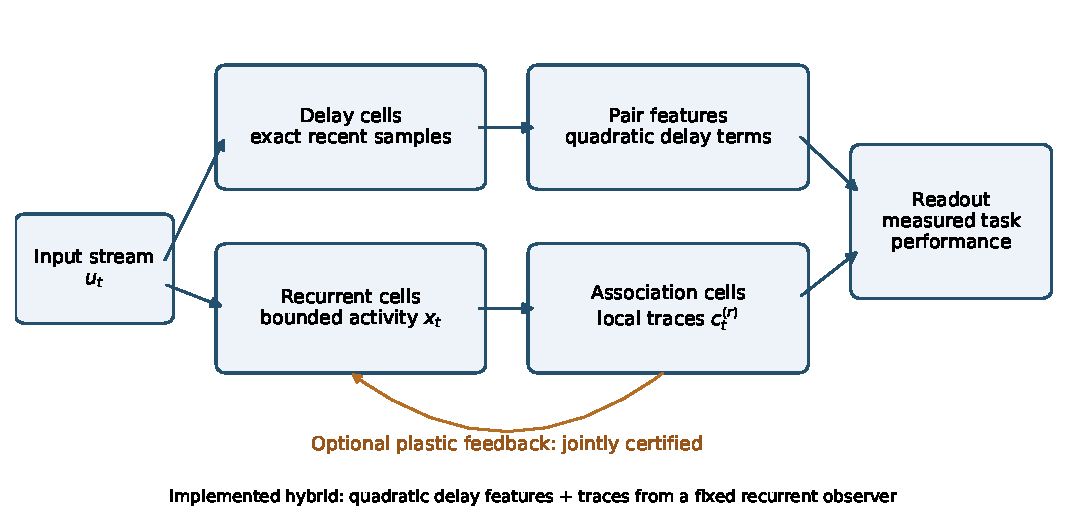
\includegraphics[width=\linewidth]{figures/architecture.pdf}
\caption{Computational branches and their roles. The plastic core permits feedback from association channels into recurrent activity. The evaluated hybrid uses traces from a fixed recurrent observer, together with explicit quadratic delay features. Training the final readout is a separate supervised procedure.}
\label{fig:architecture}
\end{figure}

\subsection{Locality, signs and resource accounting}
Equation \eqref{eq:trace} is unsupervised, but the full evaluated system includes a supervised readout. Graph construction, gains, thresholds and input encoding are designed parameters. The model permits positive and negative weights and does not enforce Dale's principle. These are computational cells rather than a validated biological neuron model.

For bounded degree $d$, the core stores $O(n+Rnd)$ values and performs $O(Rnd+nm)$ work per synchronous tick. A zero plastic weight does not eliminate the need to observe its candidate parent if the trace is still being updated. Thus active support is not a proxy for total communication cost. The implementation stores candidate edges explicitly rather than allocating an $n\times n$ matrix.

\section{Stability of the complete plastic state}
\subsection{Invariant domain and gain budget}
\begin{proposition}[Forward invariance]
For any finite input sequence, fixed finite $U,b$, and initial state $z_0\in\state$, equations \eqref{eq:activity}--\eqref{eq:trace} keep the state in $\state$.
\end{proposition}
\begin{proof}
The hyperbolic tangent lies in $[-1,1]$, so each activity update is a convex combination of two values in this interval. A product of two activities also lies in $[-1,1]$, making each trace update another such convex combination. Induction proves the claim.
\end{proof}

Define
\begin{equation}
 q=g_0+\sum_r g_r(1-\lambda_r),\qquad G=\sum_r g_r.
 \label{eq:q}
\end{equation}
In the invariant domain, $\norm{W(c)}_\infty\leq q$. For two states define $X=\norm{x-\widetilde x}_\infty$ and $C=\max_{r,ij}|c^{(r)}_{ij}-\widetilde c^{(r)}_{ij}|$. Soft thresholding and the degree normalization give
\begin{equation}
 \norm{W(c)-W(\widetilde c)}_\infty\leq GC. \label{eq:weightlip}
\end{equation}
The correlation update obeys
\begin{equation}
 |x_ix_j-\widetilde x_i\widetilde x_j|
 \leq |x_i|\,|x_j-\widetilde x_j|+|\widetilde x_j|\,|x_i-\widetilde x_i|
 \leq2X. \label{eq:productlip}
\end{equation}
This second feedback path is absent from an analysis that freezes the weights.

\subsection{A constructive contraction condition}
\begin{theorem}[Joint activity--trace contraction]\label{thm:joint}
Assume the model above and
\begin{equation}
 q+2G=g_0+\sum_r g_r(3-\lambda_r)<1. \label{eq:condition}
\end{equation}
If $G>0$, choose any $s$ satisfying $2<s<(1-q)/G$; if $G=0$, choose any $s>2$. Equip $\state$ with
\begin{equation}
 d_s(z,\widetilde z)=\max\left\{\norm{x-\widetilde x}_\infty,
 s^{-1}\max_{r,ij}|c^{(r)}_{ij}-\widetilde c^{(r)}_{ij}|\right\}. \label{eq:metric}
\end{equation}
For the same input at each tick, the transition $F_u$ satisfies
\begin{equation}
 d_s(F_u(z),F_u(\widetilde z))\leq\kappa d_s(z,\widetilde z), \label{eq:contract}
\end{equation}
where
\begin{equation}
 \kappa=\max\left\{\max_i[1-\alpha_i+\alpha_i(q+sG)],\;
 \max_r[1-\beta_r+2\beta_r/s]\right\}<1. \label{eq:kappa}
\end{equation}
\end{theorem}
\begin{proof}
Set $D=d_s(z,\widetilde z)$. Then $X\leq D$ and $C\leq sD$. Adding and subtracting $W(c)\widetilde x$ in the activity drive, and using $\norm{\widetilde x}_\infty\leq1$, bounds its difference by $qX+GC$. The 1-Lipschitz property of $\tanh$ yields
\[
 |x_i^+-\widetilde x_i^+|\leq(1-\alpha_i)X+\alpha_i(qX+GC)
 \leq[1-\alpha_i+\alpha_i(q+sG)]D.
\]
Equation \eqref{eq:productlip} similarly gives
\[
 s^{-1}|c_{ij}^{(r)+}-\widetilde c_{ij}^{(r)+}|
 \leq[1-\beta_r+2\beta_r/s]D.
\]
Taking the maximum proves \eqref{eq:contract}. The chosen interval for $s$ makes both coefficients strictly smaller than one. The proof uses global Lipschitz bounds, so it remains valid where soft thresholding is nondifferentiable and support changes.
\end{proof}

Condition \eqref{eq:condition} is sufficient and conservative. Failure to satisfy it is not proof of instability. The result controls the actual discrete recurrence; it is not obtained by numerically integrating a continuous-time stability statement. Degree normalization removes an explicit maximum-degree factor from the sufficient bound, at the cost of reducing each candidate's individual gain as degree grows.

\subsection{Consequences and limits of contraction}
For a common input sequence, repeated application gives
\begin{equation}
 d_s(z_t,\widetilde z_t)\leq\kappa^t d_s(z_0,\widetilde z_0). \label{eq:sync}
\end{equation}
On the compact invariant domain, this also constructs a unique causal state associated with a left-infinite bounded input history: initialize at increasingly remote past times and use the geometric bound to obtain a uniform Cauchy sequence. This is an echo-state property of the \emph{combined} activity and traces.

For constant input, the map has one fixed point by the contraction mapping theorem. The certified regime therefore stores history through fading transient state, rather than through multiple permanent autonomous attractors. Arbitrarily persistent episodic storage would require another mechanism. A trace that has decayed cannot be recovered merely by renaming it a latent memory.

The need to inspect the combined state can be seen in a separate counterexample. Consider
\[
 a^+=\tanh(0.5a+0.75b),\qquad b^+=\tanh(0.75a+0.5b).
\]
Each coordinate update contracts by at most $0.5$ when the other coordinate is held fixed. Along $a=b=v$, however, the map is $v^+=\tanh(1.25v)$: besides zero, it has fixed points $v\approx\pm0.710412$. Frozen-coordinate stability alone is not a joint stability argument. This example is not claimed to be an instance of the Gabriel recurrence.

\section{Perturbation bounds and robust connection labels}
\subsection{Inputs, transient corruption and persistent errors}
Let $L_u=\max_i\alpha_i\sum_k|U_{ik}|$. For two executions remaining in $\state$, with different inputs and implementation disturbances bounded in $d_s$, Theorem~\ref{thm:joint} yields
\begin{equation}
 D_{t+1}\leq\kappa D_t+L_u\norm{u_t-\widetilde u_t}_\infty+e_t. \label{eq:iss}
\end{equation}
Consequently,
\begin{equation}
 D_t\leq\kappa^tD_0+\sum_{j=0}^{t-1}\kappa^{t-1-j}
 \bigl(L_u\norm{u_j-\widetilde u_j}_\infty+e_j\bigr). \label{eq:isssum}
\end{equation}
A bounded permanent disturbance of size $e$ leads to the bound $\limsup D_t\leq e/(1-\kappa)$ when inputs agree. A one-time reset followed by the original dynamics is a transient state corruption and follows \eqref{eq:sync}. Permanent deletion of an edge changes the map; it requires a map-discrepancy bound in \eqref{eq:iss}, not an assertion of recovery to the original trajectory.

These bounds concern internal state. They become output bounds only after an output Lipschitz constant is included. They do not bound prediction error relative to an unknown target process.

\subsection{Channel support and total graph support}
For a channel, define the binary label
\begin{equation}
 A^{(r)}_{ij}(c)=\mathbf1\{|c^{(r)}_{ij}|>\lambda_r\}.
\end{equation}
If an approximate state $\widehat c$ satisfies $|c^{(r)}_{ij}-\widehat c^{(r)}_{ij}|\leq\varepsilon$, then
\begin{equation}
 \left||\widehat c^{(r)}_{ij}|-\lambda_r\right|>\varepsilon \label{eq:margin}
\end{equation}
certifies the channel's active/inactive label and, when active, its sign. This follows directly from the reverse triangle inequality. A channel inside the margin band is unresolved by that bound. Equality at the threshold is inactive by definition, but is not robust to arbitrary perturbations.

If two trajectories satisfy \eqref{eq:sync}, one may use $\varepsilon_t=s\kappa^tD_0$. If the reference has a uniform margin at least $\mu>0$ over a chosen set of times and channels, all those labels agree once $s\kappa^tD_0<\mu$. A margin measured at one time cannot guarantee agreement at every future time.

Channel support and total graph support are distinct. From \eqref{eq:weights}, an edge's weight error is bounded by
\begin{equation}
 |W_{ij}(c)-W_{ij}(\widehat c)|\leq\frac{G}{d_i}\varepsilon. \label{eq:edgeerror}
\end{equation}
A total weight whose absolute value exceeds this bound is certifiably nonzero with fixed sign. Exact inactivity of a non-backbone edge is certified when every contributing channel is certifiably inactive. Opposing channels or a backbone term can cancel, so a channel certificate alone does not classify the total edge.

\subsection{Why hard selection needs another argument}
Keeping only the largest trace is discontinuous at ties. For $v=(1+\epsilon,1)$ and $w=(1,1+\epsilon)$, top-1 selection produces outputs separated by $1+\epsilon$ in maximum norm, while $\norm{v-w}_\infty=\epsilon$. There is no uniform finite Lipschitz bound at the tie. Soft thresholding changes active support while preserving a continuous transition. A hard degree cap can be added only with a separate switching analysis or a verified selection margin; it is not covered by Theorem~\ref{thm:joint}.

\section{Local scheduling and composition}
\subsection{Fair sequential cell updates}
\begin{proposition}[Contraction per complete update window]\label{prop:async}
Partition the coordinates of $z$ into cell blocks containing $x_i$ and the incoming traces of $i$. At a microstep, replace one or more disjoint blocks by their coordinates of $F_u(z)$, leaving other coordinates unchanged. Use current neighbor values, the same input and the same schedule in the compared trajectories. If every block is updated at least once in each window of $B$ microsteps, distance decreases by at least the factor $\kappa$ per such window.
\end{proposition}
\begin{proof}
Suppose the distance at the start of a window is $D$. An unchanged coordinate has weighted error at most $D$, while every updated coordinate has error at most $\kappa D$ by the coordinate bounds in Theorem~\ref{thm:joint}. Therefore distance cannot increase during the window. Once a coordinate has been updated, subsequent updates also leave it within $\kappa D$ because all current errors remain at most $D$. At the window's end every coordinate has been updated, proving the bound.
\end{proof}

The proposition permits local update order without requiring simultaneous cell updates. It does not cover unbounded communication delays, permanently starved cells, or different input histories between the compared executions. The implementation includes a one-cell update and a random-permutation sweep experiment with input held constant within each sweep. Its temporal semantics differ from a synchronous tick and are not substituted into the task benchmark.

\subsection{Bounded-age neighbor messages}\label{sec:delayed}
Local execution requires an explicit account of which state each message represents. At microstep $t$, cell $i$ reads its current activity and incoming traces, but may receive neighbor activity
\[
 \eta_{ij,t}=x_{j,t-\delta_{ij,t}},\qquad 0\leq\delta_{ij,t}\leq L,
\]
where $L$ is an integer bound measured in microsteps. Replace $x_j$ by $\eta_{ij,t}$ in the recurrent sum and replace $x_ix_j$ by $x_{i,t}\eta_{ij,t}$ in each local trace update. The outgoing message carries activity and a timestamp; the trace block remains with its receiving cell. Histories at nonpositive times are specified as part of initialization. For simultaneous disjoint updates, all reads precede the common commit.

Convergence of asynchronous maximum-norm contractions is established theory \cite{bertsekas1991}. The following specialization states the corresponding paired-trajectory bound for the Gabriel activity--trace model, including a changing shared input.
\begin{proposition}[Forgetting with bounded message age]\label{prop:delayed}
Assume Theorem~\ref{thm:joint}, fixed parameters and the delayed local rule above. In two compared executions, use identical inputs, update schedules and message ages. Every cell must be updated within every $B$ consecutive microsteps. Let $\Delta_t$ be their weighted state distance and
\begin{equation}
 E_t=\max_{t-L\leq s\leq t}\Delta_s.
\end{equation}
Then $E_{t+1}\leq E_t$ and
\begin{equation}
 E_{t+B+L}\leq\kappa E_t,\qquad
 \Delta_t\leq E_t\leq\kappa^{\lfloor t/(B+L)\rfloor}E_0.
 \label{eq:delayed}
\end{equation}
\end{proposition}
\begin{proof}
Every coordinate read at microstep $t$ has paired weighted error at most $E_t$. A mixture of coordinates from different history times still belongs to the product state domain. The coordinate estimates used for Theorem~\ref{thm:joint} therefore bound each newly updated cell block by $\kappa E_t$. In particular, the correlation estimate uses the current local activity and the historical neighbor activity, both in $[-1,1]$. Unchanged blocks retain error at most $E_t$, which proves that the history envelope cannot increase.

Fix a starting time $t$. By time $t+B$, every block has been replaced at least once. Its error is then at most $\kappa E_t$, and later updates preserve this bound because their read errors remain at most $E_t$. At time $t+B+L$, the history envelope contains only such states. This proves the first inequality in \eqref{eq:delayed}; iteration and monotonicity give the second.
\end{proof}

For constant input, the synchronous map's unique fixed point is also a fixed history of every permitted local update. Applying the proposition to that history proves convergence to the same fixed point. For changing input, different schedules or message ages can produce different states: forgetting initialization is not invariance to communication delay. A dropped message is covered only while its retained replacement satisfies the age bound. A permanently inactive cell violates fairness. The result supplies neither automatic role reassignment after node failure nor a hardware latency or speedup guarantee.

\subsection{Feedback between certified modules}
Suppose module $a$ has metric $d_a$ and contraction factor $\kappa_a$. Let a coupling path from module $b$ to the drive of $a$ have gain $\ell_{ab}$ in these metrics, including the source output map and the receiving input map. Then module distances obey
\begin{equation}
 D_a^+\leq\kappa_aD_a+\sum_{b\ne a}\ell_{ab}D_b. \label{eq:module}
\end{equation}
If positive scalings $v_a$ satisfy
\begin{equation}
 K=\max_a\left(\kappa_a+\sum_{b\ne a}\ell_{ab}v_b/v_a\right)<1, \label{eq:modulecriterion}
\end{equation}
the complete network contracts in $\max_a D_a/v_a$. Substitution of $D_b\leq v_b\max_jD_j/v_j$ proves this statement. A spectral-radius test on the nonnegative comparison matrix supplies an alternative way to choose the weights.

This is a composition rule, not a guarantee that arbitrary connections preserve stability. In the executed two-module example, each module transmits its mean activity into the first input channel of the other, with coefficient $0.002$. The resulting uniform bound is $K=0.993615$. The experiment checks synchronization, not a performance gain from modularity.

\section{Hybrid temporal memory}
\subsection{Separating storage from adaptation}
A recurrent trace is a compressed history. It need not preserve an individual input six steps ago. For tasks requiring exact short-term storage, define a delay state of depth $D$ by
\begin{equation}
 v_t=(u_t,u_{t-1},\ldots,u_{t-D})\in\R^p,\qquad p=m(D+1). \label{eq:delay}
\end{equation}
A shift register supplies this state exactly in arithmetic appropriate to the input representation. After $D+1$ common inputs, it has forgotten all initially different contents. It is a finite-memory component, although its one-step unweighted maximum-norm gain is one.

A quadratic association bank computes
\begin{equation}
 Q(v_t)=\bigl(v_t,\{v_{a,t}v_{b,t}:1\leq a\leq b\leq p\}\bigr). \label{eq:quadratic}
\end{equation}
This is the known polynomial delay construction \cite{gauthier2021}. For bounded inputs it is bounded and Lipschitz. Pair-product cells make its computation local to the two selected delay coordinates, but the complete quadratic bank has $p(p+1)/2$ product features. Its cost is quadratic in the number of retained input coordinates.

For each recurrent observer define a readable trace statistic
\begin{equation}
 h^{(r)}_{i,t}=d_i^{-1}\sum_{j\in N_i}c^{(r)}_{ij,t}. \label{eq:readtrace}
\end{equation}
The implemented hybrid feature map is
\begin{equation}
 \phi_t=\bigl(1,Q(v_t),\{h^{(r)}_{i,t+1}\}_{i,r}\bigr). \label{eq:hybrid}
\end{equation}
Here the observer consumes $u_t$ before features are read, and its trace update uses $x_t$ as specified in \eqref{eq:trace}. In the selected hybrid the observer has fixed recurrent weights ($g_r=0$ in \eqref{eq:weights}) but continues updating its traces. Plastic feedback remains an independently implemented option, rather than a prerequisite for using trace memory.

\subsection{Memory and observability guarantees}
For identical input histories, two delay banks agree after $D+1$ updates; two recurrent observers converge by Theorem~\ref{thm:joint}. A fixed linear readout of \eqref{eq:hybrid} therefore forgets initial conditions. Before the delay banks agree, one can bound each quadratic difference by the sum of its two coordinate errors for inputs in $[-1,1]$. No autonomous readout feedback is used in the experiments; adding it requires an additional coupling bound.

The trace statistic \eqref{eq:readtrace} is a feature, not an exact state reduction. Two incoming trace rows $(a,-a)$ and $(0,0)$ have the same mean, but after thresholding they can generate different drives when the two parent activities differ. Thus mean traces and activities do not generally provide a closed reduced Markov state. Full traces remain stored by the implementation.

This separation gives distinct mechanisms for exact finite memory, nonlinear interactions and slower statistical context. The architecture is useful only insofar as these mechanisms match a task. In particular, the two polynomial diagnostic targets below are already in the delay bank's feature span. Solving them is a check of representational adequacy, not evidence that the hybrid discovers an unknown computational principle.

\section{Ordered memory on an elapsed-time clock}\label{sec:clock}
\subsection{Time variables and observation semantics}
Let $k$ count semantic input events and let $t_k$ denote their elapsed-time boundaries, with $h_k=t_{k+1}-t_k>0$. The input $u_k\in[-1,1]^2$ is held on $[t_k,t_{k+1})$. Outputs in this study are read at $t_{k+1}$, after that interval has elapsed. Holding is an explicit signal model: isolated noisy observations do not by themselves establish that the underlying physical signal stayed constant between them.

The graph recurrence and its exact delay bank advance once per declared event. Elapsed-time memory advances by $h_k$, possibly through several computational substeps. A substep is not a new observation. Conversely, two genuine consecutive events with equal values remain two events. The record therefore carries both duration and event-boundary information. Absolute clock origin and file creation time play no computational role.

Memory constants $\tau_r>0$ are measured in the same time unit as $h_k$. A forecast horizon $\eta\geq0$, when used, indexes a prediction issued from the available history; it is neither another realized time coordinate nor an observation from the future. This implementation evaluates causal reconstruction targets, not an autonomous forecasting or action-selection system.

\begin{figure}[!htbp]\centering
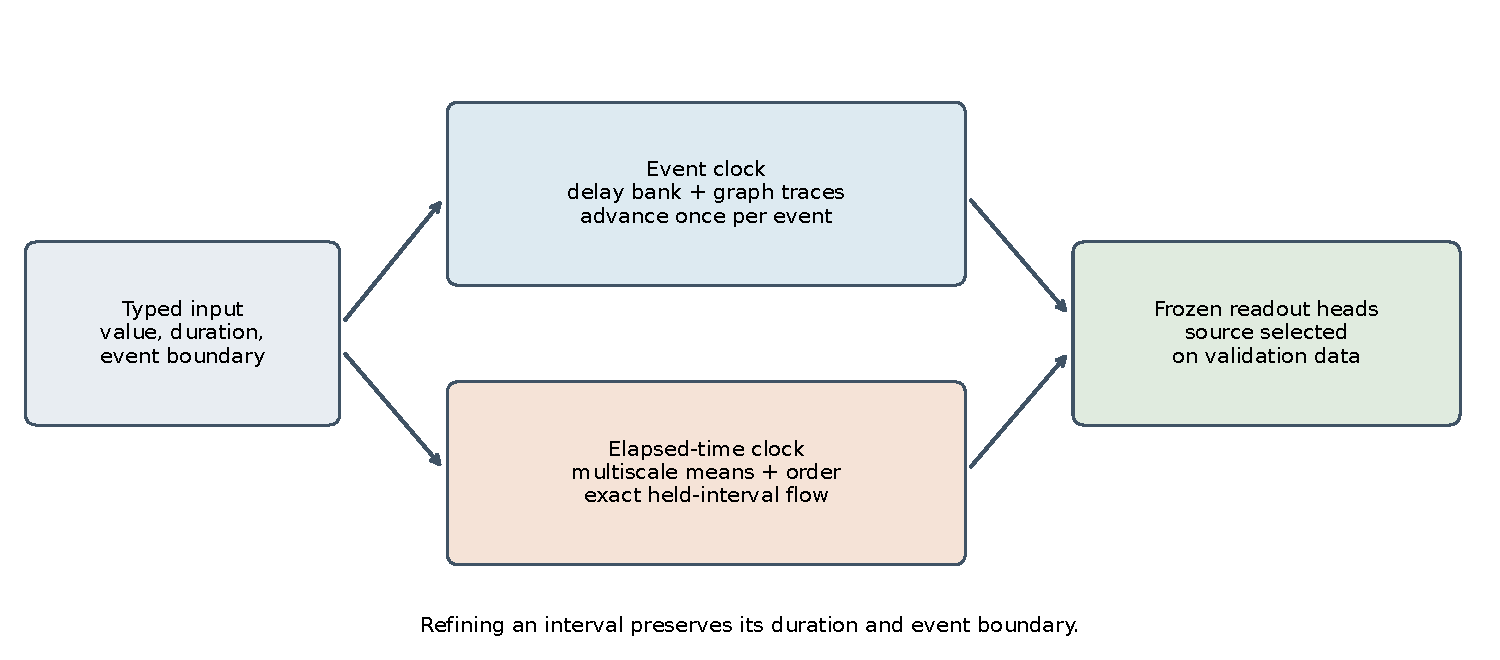
\includegraphics[width=\linewidth]{figures/multitime_architecture.pdf}
\caption{Two operational clocks with distinct semantics. The elapsed-time branch can be subdivided without altering an event. Output heads are selected on validation data and then frozen; this is offline model selection, not a learned online controller.}
\label{fig:clockarchitecture}
\end{figure}

\subsection{A normalized degree-two fading signature}
For one time constant $\tau$, write $\nu=1/\tau$ and store $a=(a_1,a_2)$ together with $r$. Define
\begin{align}
 \dot a_i&=\nu(u_i-a_i),\qquad i=1,2,\label{eq:amean}\\
 \dot r&=-2\nu r+\nu(a_1u_2-a_2u_1).\label{eq:order}
\end{align}
The term $a_1u_2-a_2u_1$ compares earlier channel content with the current input. The antisymmetry is with respect to exchange of channel identities; arbitrary reversal of a time series need not simply negate the result because the exponential weights also change.

With zero initial state at $t_0$, the coordinates are
\begin{align}
 a_i(t)&=\nu\int_{t_0}^t e^{-\nu(t-s)}u_i(s)\,ds,\\
 r(t)&=\nu^2\int_{t_0<v<s<t}
 e^{-\nu(2t-s-v)}\bigl[u_1(v)u_2(s)-u_2(v)u_1(s)\bigr]\,dv\,ds.\label{eq:orderedintegral}
\end{align}
Thus $a_i$ is the first signature level and $r$ the difference of the two ordered second-level coordinates for the integrated input path $dX_i=\nu u_i\,dt$, with scalar fading rate $\nu$ \cite{abijaber2025}. The factor $2\nu$ at level two is essential to this identification. This finite truncation does not inherit full-path reconstruction or universal approximation merely because the infinite signature has stronger properties.

\begin{proposition}[Exact interval transition and invariant box]\label{prop:held}
For fixed $u\in[-1,1]^2$ over duration $h\geq0$, set $e=\exp(-h/\tau)$. Equations \eqref{eq:amean}--\eqref{eq:order} have the exact transition
\begin{align}
 a^+&=ea+(1-e)u,\\
 r^+&=e^2r+e(1-e)(a_1u_2-a_2u_1).\label{eq:held}
\end{align}
The old value of $a$ is used. The box $|a_i|\leq1$, $|r|\leq1$ is forward invariant.
\end{proposition}
\begin{proof}
The mean equation gives $a(s)=u+e^{-\nu s}(a(0)-u)$. Its wedge with $u$ is $e^{-\nu s}(a_1(0)u_2-a_2(0)u_1)$. Substitution into the integrating-factor solution for $r$ gives \eqref{eq:held}. The mean update is convex. At $r=1$ the derivative in \eqref{eq:order} is nonpositive, and at $r=-1$ it is nonnegative, since $|a_1u_2-a_2u_1|\leq2$. These inward-pointing boundaries establish invariance, including time-varying bounded inputs.
\end{proof}

For small $h/\tau$, the implementation evaluates $1-e$ as $-\operatorname{expm1}(-h/\tau)$ to avoid subtractive cancellation. Negative durations and nonfinite values are rejected. This is an exact transition of the declared held-input model, subject only to floating-point evaluation; it is not an Euler approximation.

\begin{theorem}[Common contraction metric]\label{thm:clock}
For two trajectories under the same bounded input, define
\[
 d_{\rm c}((a,r),(\widetilde a,\widetilde r))
 =\max\{\norm{a-\widetilde a}_\infty,\tfrac12|r-\widetilde r|\}.
\]
Then $d_{\rm c}(t)\leq e^{-(t-t_0)/\tau}d_{\rm c}(t_0)$. A parallel bank of positive time constants contracts in the maximum of these metrics at rate $1/\tau_{\max}$.
\end{theorem}
\begin{proof}
Let $A_0=\norm{\delta a(t_0)}_\infty$, $R_0=|\delta r(t_0)|$ and $\Delta=t-t_0$. The difference of the mean equations gives $A(t)=e^{-\nu\Delta}A_0$. The difference of the wedge terms is at most $2A(t)$, so variation of constants gives
\[
 R(t)\leq e^{-2\nu\Delta}R_0+
 2(e^{-\nu\Delta}-e^{-2\nu\Delta})A_0.
\]
If $A_0\leq D_0$ and $R_0\leq2D_0$, the right side is at most $2e^{-\nu\Delta}D_0$. Taking the weighted maximum proves the result. The slowest rate controls the bank.
\end{proof}

Contraction removes dependence on initialization; it does not erase the distinction between different recent input orders. Nor does it establish causal influence between measured variables.

\subsection{Refinement invariance and ordered composition}
In augmented coordinates $(a_1,a_2,r,1)$ the held-input transition is the affine matrix
\begin{equation}
 M(u,h)=\begin{pmatrix}
 e&0&0&(1-e)u_1\\
 0&e&0&(1-e)u_2\\
 e(1-e)u_2&-e(1-e)u_1&e^2&0\\
 0&0&0&1
 \end{pmatrix}.\label{eq:transfer}
\end{equation}
For the same held value,
\begin{equation}
 M(u,h_2)M(u,h_1)=M(u,h_1+h_2).\label{eq:refinement}
\end{equation}
This follows either by direct multiplication or uniqueness of the autonomous flow. Products over consecutive intervals can be grouped into chunks associatively, preserving order. They generally cannot be permuted: $M(v,h_2)M(u,h_1)$ and $M(u,h_1)M(v,h_2)$ encode different histories. Numerical scheduling may reorder independent work, but must preserve these input dependencies.

An explicit separation is obtained at $\tau=1$, $h=\log2$ and zero initial state. The two inputs $(0.8,0)$ then $(0,0.4)$ end at $a=(0.2,0.2)$ and $r=0.04$. The inputs $(0,0.8)$ then $(0.4,0)$ have the same final mean but $r=-0.04$. No function of the two final mean coordinates alone can distinguish these histories. This example concerns one time scale; it does not prove that every larger bank of means fails on the same pair.

The refinement law concerns the same physical signal. Stretching a duration while keeping $\tau$ fixed intentionally changes the memory. Changing time units by $h\mapsto ch$, $\tau\mapsto c\tau$ leaves it unchanged. Inserting a true additional event intentionally changes event-index storage. These transformations must not be conflated.

\subsection{Composite state and output heads}
The implemented state combines the graph observer $(x,c)$, the event-index delay bank and independent elapsed-time coordinates $\{a^{(r)},r^{(r)}\}$. No memory-to-graph feedback is added. At each event boundary the graph consumes one input; the clock bank has already integrated its held interval. Refining any interval while retaining exactly one event boundary leaves the complete state unchanged in exact arithmetic. This statement would fail if every numerical substep also advanced the graph or delay bank.

For common semantic events, after the initial delay contents have been overwritten, the component errors satisfy
\begin{equation}
 D_{\rm graph}(K)\leq\kappa^K D_{\rm graph}(0),\qquad
 D_{\rm clock}(t)\leq e^{-(t-t_0)/\tau_{\max}}D_{\rm clock}(t_0).\label{eq:twoclocks}
\end{equation}
Here $K$ is the number of graph updates, not elapsed time. A finite-dimensional Lipschitz readout inherits these component bounds. This construction provides two explicit forgetting laws rather than pretending that an event count is a physical duration.

The bank adds $3R_{\rm c}$ state variables and $O(R_{\rm c})$ work per interval for two input channels. It is sparse in interaction order: only the antisymmetric pair coordinate is retained. More channels would introduce up to $\binom m2$ such coordinates per scale.

Output heads can use event features, elapsed features or their concatenation. For each target, the reference procedure fits each declared candidate on the training interval, selects its ridge penalty and then selects its feature family by validation mean squared error. The selected head is fixed during both test regimes. Ties follow the declared candidate order. Selection is an ordinary finite model comparison, not a proof that a target belongs uniquely to one memory type.

\section{Phase memory and retrospective conditioning}\label{sec:phase}
\subsection{A bounded rotating memory on the elapsed-time clock}
Phase and forgetting describe different aspects of a temporal representation. A purely real exponential averages a past input with a positive kernel; a rotating mode also retains a signed quadrature component. Consider $m$ bounded input channels $u_\ell(t)\in[-1,1]$ and fixed complex memory coordinates
\begin{equation}
 \dot\zeta_{j\ell}=p_j\zeta_{j\ell}+\nu_j u_\ell(t),
 \qquad p_j=-\nu_j+\mathrm i\omega_j,\quad \nu_j>0,
 \quad \omega_j\in\R.\label{eq:phaseode}
\end{equation}
Inputs and states are dimensionless. Damping $\nu_j$ and angular frequency $\omega_j$ have units of inverse time; $\tau_j=1/\nu_j$ is the forgetting time. The real implementation uses the two-coordinate matrix
\begin{equation}
 A_j=\begin{pmatrix}-\nu_j&-\omega_j\\ \omega_j&-\nu_j\end{pmatrix},
 \qquad B_j=\begin{pmatrix}\nu_j\\0\end{pmatrix}.
\end{equation}
When $\omega_j=0$ and the imaginary initial value vanishes, only one real state is needed. No spatial interpretation is required.

For a known held input over a duration $h\geq0$, the exact transition is
\begin{equation}
 \zeta^+_{j\ell}=q_j(h)\zeta_{j\ell}+b_j(h)u_\ell,
 \quad q_j(h)=e^{p_jh},\qquad
 b_j(h)=\nu_j\frac{e^{p_jh}-1}{p_j}.\label{eq:phaseexact}
\end{equation}
Since $\nu_j>0$, the denominator never vanishes. The implementation uses \texttt{expm1} for the numerator in binary64 arithmetic. This is the exact held-input discretization of a diagonal linear state-space system, rather than a new general recurrent principle \cite{gu2022diagonal,orvieto2023}.

\begin{proposition}[Disk invariance, contraction and subdivision]\label{prop:phase}
If $|\zeta_{j\ell}(0)|\leq1$ and $|u_\ell(t)|\leq1$, then $|\zeta_{j\ell}(t)|\leq1$. Two trajectories driven by the same input satisfy
\begin{equation}
 |\zeta_{j\ell}(t)-\widetilde\zeta_{j\ell}(t)|
 =e^{-\nu_j(t-s)}|\zeta_{j\ell}(s)-\widetilde\zeta_{j\ell}(s)|.\label{eq:phasecontract}
\end{equation}
Splitting a held interval into any finite set of nonnegative durations with the same total duration leaves its transition unchanged.
\end{proposition}
\begin{proof}
Variation of constants gives
\[
 |\zeta(t)|\leq e^{-\nu(t-s)}|\zeta(s)|+
 \nu\int_s^t e^{-\nu(t-v)}|u(v)|\,dv\leq1.
\]
Subtracting two copies of the differential equation cancels the common input, leaving $\delta\zeta(t)=e^{p(t-s)}\delta\zeta(s)$ and hence \eqref{eq:phasecontract}. Finally, $q(h+k)=q(k)q(h)$ and $b(h+k)=q(k)b(h)+b(k)$. Applying these identities repeatedly proves subdivision.
\end{proof}

The bank contracts in $\max_{j,\ell}|\delta\zeta_{j\ell}|$ with rate $\min_j\nu_j$, independently of the frequencies. Increasing a frequency does not increase its memory half-life. For different inputs,
\begin{equation}
 |\delta\zeta_{j\ell}(t)|\leq e^{-\nu_j(t-s)}|\delta\zeta_{j\ell}(s)|
 +\nu_j\int_s^t e^{-\nu_j(t-v)}|\delta u_\ell(v)|\,dv.\label{eq:phaseiss}
\end{equation}
The implemented optional bank runs in parallel with the graph; no feedback from the bank into the graph is added. The graph advances once per event while the bank advances by the declared duration. Its common-input bound composes directly with the graph bound and can likewise be combined with the independent ordered-memory bound. The evaluated hybrid heads concatenate the bank and trace features. A change of time units, $h\mapsto sh$, $\nu\mapsto\nu/s$, $\omega\mapsto\omega/s$, preserves \eqref{eq:phaseexact}. Changing only durations describes a different signal-processing experiment.

Using a generic numerical step can destroy these guarantees. Forward Euler has a homogeneous multiplier $1-\nu h+\mathrm i\omega h$, whose modulus is less than one only for $0<h<2\nu/(\nu^2+\omega^2)$. For $\nu=1$, $\omega=4$, $h=0.2$, its modulus is approximately $1.1314$, whereas the exact transition has modulus $0.8187$.

\subsection{What an expanding spiral measures}
For a nonzero common-input state difference and $\omega_j\neq0$, use a continuous, unwrapped phase. Then
\begin{equation}
 r(t)=r(0)e^{-\nu_jt},\quad \theta(t)=\theta(0)+\omega_jt,
 \qquad r=r(0)\exp\!\left[-\frac{\nu_j}{\omega_j}(\theta-\theta(0))\right].\label{eq:logspiral}
\end{equation}
This is a logarithmic spiral of a state difference. An individual driven trajectory need not have monotone radius or phase. The familiar flared geometry arises when this evolution is viewed backwards, but it then measures inverse sensitivity.

Suppose the intervening input is known and subtracted from the solution, and the present complex state is known only to an isotropic error radius $\sigma>0$. The inverse transition over age $a\geq0$ multiplies the error disk by $e^{-p_ja}$. Its exact unconstrained radius is
\begin{equation}
 R_j(a)=\sigma e^{\nu_ja}.\label{eq:trumpet}
\end{equation}
This is absolute amplification of additive state error. The Euclidean relative matrix condition number of a single damped rotation is one. For a bank, its homogeneous transition has singular values $e^{-\nu_ja}$, hence relative condition number $e^{(\max_j\nu_j-\min_j\nu_j)a}$. Unequal damping can therefore add anisotropy to the absolute inverse sensitivity.

Rotation changes the orientation of an error vector, but not the disk. Plotting age against its two error coordinates produces an expanding tube; following one rotating error vector produces a spiral on that surface. A prior state constraint can truncate this disk. For a prescribed radius tolerance $\varepsilon\geq\sigma$, the untruncated bound permits ages
\begin{equation}
 a\leq \nu_j^{-1}\log(\varepsilon/\sigma).\label{eq:phasehorizon}
\end{equation}
Thus forward forgetting and backward reconstruction sensitivity are two directions of the same transition. Equation~\eqref{eq:trumpet} is conditional on known forcing; it does not reconstruct missing inputs or uniquely identify a history from a finite memory state. Results on finite-width delayed copying likewise distinguish memory range from reconstruction resolution \cite{francois2025}. Their statistical approximation setting is different from the present deterministic inverse-state calculation.

The source spiral and phase-memory specifications motivate a joint treatment of phase, scale and access \cite{klemm2025oriphiel,klemm2025spiral}. The operational objects here are the explicit state transition, its output map and its uncertainty set. A visual curve or a low similarity distance alone does not establish dynamical closure, semantic identity or correct retrieval.

\subsection{Five coordinates as a testable memory budget}
A five-coordinate bank is obtained from one real fading coordinate and two complex modes. In the evaluated family their damping rates are $1,4,1$ in normalized record time; the two complex modes have angular frequencies $16,4$. This gives five real coordinates per input channel. The three-coordinate family retains the real mode and the first complex mode; the seven-coordinate family adds the pair $(\nu,\omega)=(16,64)$. These are fixed candidate representations, not assertions that every dynamical system has five effective degrees of freedom.

An exact local smooth state representation has a basic dimension constraint. If an open subset of $\R^d$ admits differentiable encoding $F$ into $\R^p$ and decoding $G$ with $G\circ F=\operatorname{id}$, the chain rule gives
\begin{equation}
 I_d=DG(F(x))DF(x),\qquad d\leq p.\label{eq:dimensionbound}
\end{equation}
Consequently five smooth coordinates cannot exactly retain six independently variable state coordinates. Conversely a scalar fading state needs only one. Output-specific reductions can require fewer coordinates than the full state, but must satisfy the closure and output conditions in Section~\ref{sec:invariants}. An optimal approximate budget further requires a task loss, accuracy tolerance and resource cost. The implemented $3/5/7$ comparison examines a particular family; it neither optimizes all five-dimensional models nor measures the full Gabriel system's dimension.

\subsection{Exact affine uncertainty ranges for the phase bank}
Let $0=t_0\leq\cdots\leq t_N=T$ be fixed interval endpoints, $h_i=t_i-t_{i-1}$, and let each $u_{i\ell}$ be held over its interval. With a known initial state,
\begin{align}
 \zeta_{j\ell}(T)&=e^{p_jT}\zeta_{j\ell}(0)+\sum_{i=1}^N K_{ij}u_{i\ell},\\
 K_{ij}&=e^{p_j(T-t_i)}\nu_j\frac{e^{p_jh_i}-1}{p_j}.\label{eq:phasekernel}
\end{align}
A frozen affine readout of real and imaginary state coordinates therefore compiles to $f_a(u)=b_a+\sum_q c_{qa}u_q$, where $q$ indexes event-channel pairs and the known initial contribution is included in $b_a$.

For independent intervals $u_q\in[\ell_q,h_q]$, put $\mu_q=(\ell_q+h_q)/2$, $r_q=(h_q-\ell_q)/2$, $d_0=b_a-b_b$ and $d_q=c_{qa}-c_{qb}$. Every pairwise score difference has the exact range
\begin{equation}
 f_a-f_b\in\left[
 d_0+\sum_q d_q\mu_q-\sum_q|d_q|r_q,\;
 d_0+\sum_q d_q\mu_q+\sum_q|d_q|r_q
 \right].\label{eq:phasebox}
\end{equation}
Each endpoint is attained by choosing each independent variable at the appropriate end of its interval. A class whose lower differences against all rivals are strictly positive is the unique winner throughout the box. This special case needs no vertex enumeration, nonlinear relaxation or finite hypothesis catalogue. It uses the established affine support function with the compiled held-input kernel.

The same unresolved variable may appear in several computational pieces of a held interval. Its coefficients must be added before the absolute value is taken. For instance, $v-v$ has zero width for a shared unknown $v\in[-1,1]$, whereas replacing it by independent $v_1-v_2$ yields width four. Keeping the same uncertainty identity under subdivision preserves both the transition and the exact range.

For one scalar affine target and equal-cost exact queries, reading a variable reduces the full interval width by $2|d_q|r_q$, independent of the response. Selecting the largest such terms minimizes remaining worst-case width for a given number of queries. It need not minimize the response-dependent time to a decision, and different class pairs generally prefer different variables. The implemented multiclass policy uses the maximum absolute pair coefficient as a fixed heuristic, compared with reverse temporal order.

The mathematical interval endpoints are exact; the binary64 query loop is not directed rounding. Every reported stop is subsequently re-evaluated using Arb, including kernel exponentials, fitted coefficients, pair differences and the sum of absolute coefficients over all unread scalars. The resulting certificate covers the continuous declared box for these linear heads. Hybrids containing the nonlinear trace observer receive validated complete-input point predictions only in this extension; they do not inherit \eqref{eq:phasebox}.

\section{Information-preserving transformations and their limits}\label{sec:invariants}
\subsection{Invariance is relative to a declared transformation}
The architecture has several distinct guarantees. The state box is forward invariant; a simultaneous relabeling of cells and all incident parameters is equivariant; elapsed-time origin is irrelevant; and splitting a held interval preserves its transition. Memory values themselves are generally not conserved. Input reversal, graph rewiring, projection and quantization each require separate analysis.

For example, let a cell permutation relabel $x$, every incoming trace, $B$, $U$, $b$, $\alpha$ and the parent identities consistently. The transformed graph update is the permutation of the original update, because sparse sums, pointwise nonlinearities and edgewise products commute with relabeling. Relabeling only an unweighted graph while retaining its input ports or heterogeneous parameters does not have this property. Graph isomorphism alone is therefore insufficient to identify computational states.

\subsection{When a compression is a dynamical reduction}
Let $P:Z\to\bar Z$ be a surjection. A transition $F_u$ induces a well-defined reduced transition $\bar F_u$ exactly when
\begin{equation}
 Pz=P\widetilde z\quad\Longrightarrow\quad PF_u(z)=PF_u(\widetilde z)
 \quad\text{for every admissible }u.\label{eq:congruence}
\end{equation}
Necessity follows from $PF_u=\bar F_uP$. For sufficiency, define $\bar F_u(\bar z)=PF_u(z)$ using any representative; \eqref{eq:congruence} makes the definition independent of that choice. Outputs must also factor through $P$ if reduced trajectories are to preserve their meaning.

Equal present observations do not establish \eqref{eq:congruence}. Take $F(z)=\operatorname{diag}(0.2,0.8)z$ and $P(z)=z_1+z_2$. States $(1,-1)$ and $(0,0)$ have the same projection, but their next projections are $-0.6$ and $0$. Both full trajectories are contractive. This is why compressed trace statistics remain readout features rather than replacing stored traces.

A reconstruction residue can close an encoding contract $\operatorname{Dec}(Y,R)=X$ for a specified source object. It must be stored and costed. If a finite-precision internal memory has at most $N$ states, exact recovery of every length-$T$ history over an alphabet of size $K$ requires $N\geq K^T$, unless additional storage is supplied. This is the pigeonhole principle. A bounded fading state and an append-only archive serve different functions; deterministic replay from saved inputs does not make the internal state a lossless archive.

\subsection{Why feedback validation must inspect the right object}
Serialization round trips, threshold acceptance and dynamical stability certify different properties. For example, gating the contraction $T(z)=z/2$ by acceptance only when the first coordinate does not decrease freezes every point with $z_1>0$. A monotone Boolean-coordinate swap $(z_1,z_2)\mapsto(z_2,z_1)$ has a two-cycle, despite possessing fixed points. Neither a score gate nor fixed-point existence alone establishes convergence. The contraction results in this work apply to the stated state transition; they are not inherited by an arbitrary adaptive gate placed around it.

\section{Partial observation and selective acquisition}\label{sec:partial}
\subsection{Conditional statements over input completions}
Consider a buffered window of $N$ held-input events. Durations, time constants and the elapsed-time state immediately before the window are known. Each scalar input belongs to a closed interval; exact observations are singleton intervals. The admissible history set is the nonempty Cartesian box
\begin{equation}
 \mathcal B=\prod_{j=1}^{N}\prod_{i=1}^{2}[\underline u_{ji},\overline u_{ji}]
 \subseteq[-1,1]^{2N}.\label{eq:inputbox}
\end{equation}
This is a set of possible completions, not a probability distribution. A missing entry is not assigned zero. If observations contradict the bounds, the evidence is inconsistent and no output claim is issued. In particular, universal predicates over an empty feasible set must not be used to certify either truth value.

Let $f(u)$ be a scalar output of the specified model and let
\begin{equation}
 L(\mathcal B)=\min_{u\in\mathcal B}f(u),\qquad
 U(\mathcal B)=\max_{u\in\mathcal B}f(u).\label{eq:range}
\end{equation}
For the predicate $f(u)>0$, a positive lower bound establishes value 1, a nonpositive upper bound establishes value 0, and a range crossing the decision boundary requires abstention. The implementation uses a conservative numerical margin: it reports 1 for $L>10^{-12}$, 0 for $U<-10^{-12}$ and \texttt{NoBit} otherwise. This predicate-level uncertainty is distinct from declaring that an object belongs to an unknown catalog class.

The range concerns the complete-input model output. If a separate bound $|y-f(u)|\leq\epsilon_{\rm model}$ is available for an external target, its interval expands to $[L-\epsilon_{\rm model},U+\epsilon_{\rm model}]$. No such universal target-error bound is estimated here. Likewise, a fully observed prefix gives a known model initialization; an uncertain earlier history requires its own propagated set and is outside the exact initialization contract used below.

\subsection{Multiaffine structure of ordered memory}
For one scale, put $d=\exp(-T/\tau)$, where $T=\sum_j h_j$, and define the final mean weight of event $j$ by
\begin{equation}
 w_j=(1-e^{-h_j/\tau})\exp\left(-\frac1\tau\sum_{\ell=j+1}^{N}h_\ell\right).
\end{equation}
Write $v\wedge u=v_1u_2-v_2u_1$. With known initial coordinates $(a_0,r_0)$, repeated application of \eqref{eq:held} gives
\begin{align}
 a_N&=d a_0+\sum_jw_ju_j,\label{eq:weightedmean}\\
 r_N&=d^2r_0+d\sum_j w_j(a_0\wedge u_j)
       +\sum_{i<j}w_iw_j(u_i\wedge u_j).\label{eq:weightedorder}
\end{align}
The formulas follow by induction: a new event multiplies preceding weights by its decay and adds its own $(1-e)$ weight. The ordered update adds only interactions between the new event and preceding mean content. No within-event quadratic term occurs.

Consequently each scalar coordinate is affine in any one scalar input when all other inputs are fixed. This property is called multiaffinity. It survives affine combinations across scales, addition of current-input coordinates and a known duration feature. The eligible readout is therefore
\begin{equation}
 f(u)=c^\top(1,u_N,\log h_N,\{a_N^{(r)},r_N^{(r)}\}_r).\label{eq:auditedhead}
\end{equation}
Its coefficients are fixed before acquisition. This includes the elapsed ordered head defined in Section~\ref{sec:clock}. The nonlinear graph recurrence, squared delay features and uncertainty in durations or time constants do not inherit this multiaffine argument.

\begin{proposition}[Exact conditional range]\label{prop:vertex}
Under \eqref{eq:inputbox} and the fixed-parameter assumptions above, the extrema of \eqref{eq:auditedhead} occur at vertices of $\mathcal B$. If $J$ scalar fields have nonzero interval width, at most $2^J$ evaluations determine \eqref{eq:range} exactly in real arithmetic.
\end{proposition}
\begin{proof}
Equations \eqref{eq:weightedmean}--\eqref{eq:weightedorder} establish multiaffinity. For an interior value of any one variable, $f$ is a convex combination of its two endpoint values with the other coordinates unchanged. Applying this successively to all $J$ variables expresses $f(u)$ as a convex combination of vertex values. Thus no interior value exceeds the vertex maximum or falls below the vertex minimum. The vertices belong to the box, so both bounds are attained. This is the standard vertex principle \cite{blanchini2022}, applied to the explicit memory readout.
\end{proof}

For a finite window, batched replay costs $O(NR_{\rm c}2^J)$ operations. The reference allocates $O((N+R_{\rm c})2^J)$ working values and retains a scalar $2^J$ vertex array for each audited head. It rejects requests above its declared limit of 16 missing scalars. The exponential dependence is explicit; no efficient solution for an arbitrarily incomplete stream is claimed. Extra correlations between missing inputs can invalidate exactness of a rectangular feasible set, although a containing box still gives an outer range.

\subsection{Preserving dependencies across refinement and repeated observations}
The unknown for a held interval is its input value, not a fresh unknown at every computational substep. Replaying each vertex with the same value throughout a subdivision preserves \eqref{eq:refinement}, and hence preserves the output range. Treating the substeps as independent unknown inputs would describe a larger family of signals.

Even ordinary interval propagation through two substeps can discard this dependency. For a single unknown input in $[-1,1]^2$, zero initial state, $\tau=1$ and $h=\log2$, the true ordered coordinate is identically zero: a constant input has no temporal ordering with another direction. One unsplit interval update returns $[0,0]$. Replacing the intermediate reachable state by its coordinate box and then propagating another half interval gives approximately $[-0.12132,0.12132]$. This is a conservative enclosure, but its width is an artifact of dependency loss. Vertex replay with a shared input variable returns zero for both subdivisions.

A second copy of the same exact observation imposes the same constraint and cannot shrink the feasible set again. The implementation binds acquisitions to their event/channel coordinate, treats identical repeated values idempotently and rejects conflicting duplicates. This is a concrete constraint-identity rule; it does not identify statistical independence by counting views or taking the rank of an unspecified dependency graph.

\subsection{One-query minimax acquisition}\label{sec:query}
Assume a query returns the exact value of one missing coordinate of an immutable buffered record, at unit cost. This is retrieval from a retained record, not a sensor capable of measuring an unrecorded past signal. Acquiring a value neither changes the input history nor retrains the readout. Let $\mathcal B_{j=v}$ be the box with coordinate $j$ fixed at $v$, and write its output width as
\[
 W_j(v)=U(\mathcal B_{j=v})-L(\mathcal B_{j=v}).
\]
\begin{proposition}[Endpoint formula for worst remaining width]\label{prop:query}
For a multiaffine scalar $f$ on a box,
\begin{equation}
 \max_{v\in[\underline u_j,\overline u_j]}W_j(v)
 =\max\{W_j(\underline u_j),W_j(\overline u_j)\}.\label{eq:querywidth}
\end{equation}
Selecting the coordinate minimizing the right side is optimal for the worst-case width after one exact, unit-cost query.
\end{proposition}
\begin{proof}
For fixed $v$, the extrema over remaining variables occur at their vertices. Hence
\[
 W_j(v)=\max_{p,q\in\operatorname{Vert}(\mathcal B_{-j})}
               [f(v,p)-f(v,q)].
\]
Each bracket is affine in $v$, so their maximum is convex. A convex function on an interval is bounded above by the larger endpoint value; equality is attained at an endpoint. Minimizing this exact worst-case cost over available coordinates proves the final statement.
\end{proof}

If the acquired value has normalized position $s=(v-\underline u_j)/(\overline u_j-\underline u_j)$, the new vertex array is obtained directly from paired faces:
\begin{equation}
 f(v,p)=(1-s)f(\underline u_j,p)+s f(\overline u_j,p).\label{eq:restrictvertices}
\end{equation}
No new trajectory fit or full vertex replay is needed. All candidate scores cost $O(J2^J)$ using the stored array; restriction halves it. Repeating this rule gives an adaptive greedy policy. It is not asserted to minimize total acquisition cost or to be globally optimal over several future queries. In particular, minimizing worst-case width and maximizing the probability of resolving a sign are different objectives.

Every acquired value restricts the feasible set, so the exact range can only narrow while retaining the complete-input output if the declared bounds are correct. This set inclusion is not a strict contraction rate and does not require a probability distribution. The acquisition layer issues queries and conditional output reports; it leaves the Gabriel state-transition law and its contraction certificate unchanged.

\section{Polynomial-cost bounds for larger missing sets}\label{sec:scalable}
\subsection{Compiling a multichannel ordered readout}
Vertex enumeration preserves exact extrema but its $2^J$ storage prevents long missing-data windows. The degree-two structure permits a smaller exact representation, followed by a conservative scalar enclosure. Keeping shared variables in polynomial set representations is an established technique, including sparse polynomial zonotopes \cite{kochdumper2021}. The construction here uses explicit quadratic coefficients; it is not a new general-purpose set representation.

For $m$ input channels, retain one mean per channel and one ordered coordinate $r_{ab}$ for each $a<b$ at each fading scale. On an interval of length $h$, put $e=\exp(-h/\tau)$ and use
\begin{align}
 a_c^+&=ea_c+(1-e)u_c,\\
 r_{ab}^+&=e^2r_{ab}+e(1-e)(a_au_b-a_bu_a).
 \label{eq:multiordered}
\end{align}
Every pair obeys the two-channel bounds already derived. Taking the maximum over channels and pairs preserves that contraction estimate; the number of retained coordinates per scale is $m+\binom m2$.

Consider $N$ held intervals, known positive durations $h_j$, endpoints $t_j=\sum_{i\leq j}h_i$ and $T=t_N$, with zero initial memory. Define
\begin{equation}
 w_j^{(\tau)}=(1-e^{-h_j/\tau})e^{-(T-t_j)/\tau}.
\end{equation}
Unrolling \eqref{eq:multiordered} gives
\begin{align}
 a_c(T)&=\sum_j w_j^{(\tau)}u_{jc},\\
 r_{ab}(T)&=\sum_{i<j}w_i^{(\tau)}w_j^{(\tau)}
       (u_{ia}u_{jb}-u_{ib}u_{ja}).\label{eq:polynomialarea}
\end{align}
To verify the second expression, expand $a(t_{j-1})$ in the forcing of interval $j$ and propagate the resulting area through later intervals with squared decay. The coefficient of a pair $i<j$ is
$(1-e^{-h_i/\tau})(1-e^{-h_j/\tau})
e^{-(t_j-t_i)/\tau}e^{-2(T-t_j)/\tau}$,
which equals $w_i^{(\tau)}w_j^{(\tau)}$. A held interval creates no interaction with itself.

Consequently an affine head on the final input, means and ordered coordinates has the exact polynomial form
\begin{equation}
 f(v)=c+b^\top v+\tfrac12v^\top Qv,
 \qquad Q=Q^\top,\quad Q_{ii}=0,\label{eq:quadratichead}
\end{equation}
where $v$ lists scalar inputs in event/channel order. The compiler sums the antisymmetric channel coefficients in \eqref{eq:polynomialarea} across scales. A known nonzero initialization adds known constant and linear terms, but the supplied compiler and external experiments use zero initialization. Durations, parameters and readout coefficients are fixed during the audit. No analogous quadratic representation is claimed for the nonlinear recurrent observer.

\subsection{An enclosure that survives exact observations}
For a box $v=\mu+\rho\odot z$, $z\in[-1,1]^J$, substitute known coordinates and retain only positive radii. Here $\odot$ denotes coordinatewise multiplication. Equation~\eqref{eq:quadratichead} becomes
\begin{equation}
 f=C+\ell^\top z+\sum_{i<j}\widetilde Q_{ij}z_iz_j,
 \quad C=f(\mu),\quad
 \ell=\rho\odot(b+Q\mu),\quad
 \widetilde Q_{ij}=\rho_iQ_{ij}\rho_j.\label{eq:centered}
\end{equation}
All indices on the right are restricted to the missing coordinates after the full center has been substituted. The triangle inequality gives the outer range
\begin{equation}
 [\underline f,\overline f]=[C-R,C+R],\qquad
 R=\sum_i|\ell_i|+\sum_{i<j}|\widetilde Q_{ij}|.
 \label{eq:coefficientrange}
\end{equation}
This enclosure is generally wider than the exact range: $z_1z_2+z_1z_3+z_2z_3$ has range $[-1,3]$ on the cube, whereas \eqref{eq:coefficientrange} gives $[-3,3]$. The polynomial retains variable identities, but its scalar enclosure does not exploit every compatibility constraint among monomial signs.

An exact query returning $z_j=s\in[-1,1]$ updates the coefficients by
\begin{equation}
 C'=C+\ell_js,\qquad
 \ell'_i=\ell_i+\widetilde Q_{ij}s\quad(i\ne j),\qquad
 \widetilde Q'=\widetilde Q_{-j,-j}.\label{eq:polyquery}
\end{equation}
Thus the smaller polynomial remains exact. Its enclosure is nested inside the preceding enclosure: if $R'$ is the new radius, then
\[
 |C'-C|+R'
 \leq |\ell_j||s|+\sum_{i\ne j}(|\ell_i|+|\widetilde Q_{ij}||s|)
             +\sum_{i<k;\,i,k\ne j}|\widetilde Q_{ik}|\leq R.
\]
The resulting class or sign report therefore remains valid under subsequent compatible observations in exact arithmetic. Identical repeated observations are idempotent; conflicting values are rejected.

\subsection{Selecting queries using the enclosure}
After fixing coordinate $j$ at $s$, its enclosing width is
\begin{equation}
 \overline W_j(s)=2\left(\sum_{i\ne j}|\ell_i+\widetilde Q_{ij}s|
                     +\sum_{i<k;\,i,k\ne j}|\widetilde Q_{ik}|\right).
 \label{eq:polywidth}
\end{equation}
It is convex in $s$, so its maximum occurs at $s=\pm1$. For $P$ specified scalar outputs, minimize
\begin{equation}
 j_*\in\arg\min_j\max_{1\leq p\leq P}
       \max\{\overline W_{p,j}(-1),\overline W_{p,j}(1)\}.
 \label{eq:polypolicy}
\end{equation}
This is an exact one-query minimax rule for the chosen \emph{enclosing widths}. It is a surrogate for the exact reachable widths of Section~\ref{sec:query}, and does not minimize the number of queries needed to resolve a class. All candidate scores cost $O(PJ^2)$ using row sums of the absolute quadratic matrices, with $O(PJ^2)$ storage. The reference copies the remaining matrices after substitution. Initial compilation stores matrices over all $Nm$ input coordinates and costs quadratic space in $Nm$; no constant-memory claim is made for an unbounded record.

For $K$ class scores $f_a$, audit all $P=\binom K2$ pairwise differences. A class $a$ is resolved when every enclosing lower bound for $f_a-f_b$, $b\ne a$, is strictly positive. Otherwise the method abstains. This proves the same winner as the complete-input head for every compatible completion. It does not prove that the head's winner equals the external class label. The implemented decision margin is $10^{-10}$; arithmetic is float64, without outward rounding.

\section{Bounding the nonlinear trace observer}\label{sec:observeraudit}
\subsection{Finite-record model and exact trace elimination}
The preceding polynomial representation does not describe a recurrent $\tanh$ network. A different construction applies to the fixed trace observer. Throughout this section, parameters and candidate parents are fixed, updates are synchronous, inputs satisfy $u_t\in[-1,1]^m$ for $t=0,\ldots,N-1$, and $x_0=c_0=0$. Let $A=\operatorname{diag}(\alpha)$ and write
\begin{equation}
 d_t=Bx_t+Uu_t+b,\qquad x_{t+1}=(I-A)x_t+A\tanh(d_t).
 \label{eq:observertransition}
\end{equation}
Traces follow the original recurrence, using $x_t$, not $x_{t+1}$. They are readable but do not affect $B$. This is not a verifier for plastic feedback, uncertain initialization or delayed execution.

For one scalar output, including a class-score difference, collect its fixed head coefficients as
\begin{equation}
 f(u)=h_0+h_u^\top u_{N-1}+h_x^\top x_N
       +\sum_{r,i}h^{(r)}_i\frac1{d_i}\sum_{j\in N_i}c^{(r)}_{ij,N}.
 \label{eq:observerhead}
\end{equation}
Unrolling the linear trace filter gives
\begin{align}
 c^{(r)}_{ij,N}&=\sum_{t=0}^{N-1}\beta_r(1-\beta_r)^{N-1-t}x_{i,t}x_{j,t},\\
 w_{i,t}&=\frac1{d_i}\sum_r h^{(r)}_i\beta_r(1-\beta_r)^{N-1-t}. \label{eq:tracecompile}
\end{align}
Define $(W_t)_{ij}=w_{i,t}$ for $j\in N_i$, zero otherwise, and $M_t=W_t+W_t^\top$. Then
\begin{equation}
 f(u)=h_0+h_u^\top u_{N-1}+h_x^\top x_N
                    +\frac12\sum_{t=0}^{N-1}x_t^\top M_tx_t.
 \label{eq:observerhistory}
\end{equation}
This identity eliminates trace variables from the scalar audit without changing the model. Terms from different trace scales and reciprocal directed edges are combined before taking absolute values or interval products. Such combination retains cancellations that would be lost by treating each trace output independently. The implemented graph has no self-edges, so diagonal quadratic terms are absent. The identity remains valid with self-edges, but that variant is not implemented here. Equation~\eqref{eq:observerhistory} is quadratic in the \emph{state history}, not in the input record.

\subsection{Forward boxes and interval reverse derivatives}
Let $\mathcal B=[\underline u,\overline u]$ be a Cartesian input box. A fixed affine map has interval image enclosed by
\[
 C[z]=[C^+\underline z+C^-\overline z,\ C^+\overline z+C^-\underline z],
 \quad C^+=\max(C,0),\quad C^-=\min(C,0).
\]
Products use the minimum and maximum of the four endpoint products. Monotonicity of $\tanh$ then yields forward activity boxes $[x_t]$ and preactivation boxes $[d_t]$. Propagating the original trace recurrence and applying \eqref{eq:observerhead} produces a basic enclosure $I_{\rm basic}$. Evaluating the compiled expression \eqref{eq:observerhistory} on the same activity boxes gives $I_{\rm hist}$. Set $I_{\rm structured}=I_{\rm basic}\cap I_{\rm hist}$. Both calculations ignore some dependencies between uncertain states; neither is an exact reachable-set calculation.

For derivative bounds, first consider the exact reverse recurrence. With terminal cotangent $\ell_N=h_x$ and $D_t=\operatorname{diag}(\operatorname{sech}^2d_t)$,
\begin{align}
 v_t&=AD_t\ell_{t+1},\\
 \nabla_{u_t}f&=U^\top v_t+\mathbf1_{\{t=N-1\}}h_u,\\
 \ell_t&=M_tx_t+(I-A)\ell_{t+1}+B^\top v_t.
 \label{eq:observeradjoint}
\end{align}
The term $M_tx_t$ is the derivative of the already combined trace contribution at time $t$. It must not be dropped when auditing a trace readout.

For a scalar interval $[a,b]$, put $d_{\min}=\max(0,a,-b)$ and $d_{\max}=\max(|a|,|b|)$. Then
\[
 \operatorname{sech}^2([a,b])\subseteq
 [1-\tanh^2(d_{\max}),\ 1-\tanh^2(d_{\min})].
\]
Evaluating \eqref{eq:observeradjoint} with these slope intervals and the forward state boxes encloses every input derivative over $\mathcal B$. Write the resulting absolute derivative bounds, flattening event/channel indices to $j$, as
\begin{equation}
 L_j(\mathcal B)=\max\{|\underline{\partial_jf}|,|\overline{\partial_jf}|\}.
 \label{eq:observergain}
\end{equation}
They are bounds over the whole box, not gradients sampled only at its midpoint. In particular, a small point gradient is not itself a robustness certificate.

\begin{proposition}[Finite-record enclosures and compatible refinement]\label{prop:observerbox}
Under the fixed-parameter and initialization assumptions above, let $\bar u$ and $r$ be the midpoint and half-widths of $\mathcal B$. In exact real arithmetic,
\begin{equation}
 I_{\rm mv}(\mathcal B)=\left[f(\bar u)-\mathcal R(\mathcal B),\ f(\bar u)+\mathcal R(\mathcal B)\right],
 \qquad \mathcal R(\mathcal B)=\sum_jL_j(\mathcal B)r_j
 \label{eq:observermv}
\end{equation}
contains all values of $f$ on $\mathcal B$. The intersection
\[
 I_{\rm hybrid}=I_{\rm basic}\cap I_{\rm hist}\cap I_{\rm mv}
\]
is a valid enclosure. Each of these intersections and $I_{\rm mv}$ is nested under compatible restriction to a smaller Cartesian input box.
\end{proposition}
\begin{proof}
Forward inclusion follows by induction through the affine, monotone and product operations. The trace-filter identity is exact. The chain rule gives \eqref{eq:observeradjoint}; backward interval induction therefore encloses its cotangents and input derivatives. Integrating the gradient along the segment from $\bar u$ to any $u\in\mathcal B$ proves \eqref{eq:observermv}. Convexity of the box ensures that the whole segment is covered.

Every interval operation used here preserves set inclusion, including the exact scalar slope range. Hence a subbox $\mathcal B'$ has smaller forward and backward intervals, and $L_j(\mathcal B')\leq L_j(\mathcal B)$. Its midpoint and radii satisfy $|\bar u'_j-\bar u_j|+r'_j\leq r_j$. Applying the old derivative bound along the midpoint segment gives
\[
 |f(\bar u')-f(\bar u)|+\sum_jL_j(\mathcal B')r'_j
 \leq\sum_jL_j(\mathcal B)(|\bar u'_j-\bar u_j|+r'_j)
 \leq\mathcal R(\mathcal B).
\]
This proves centered-interval nesting. Forward and compiled interval evaluation are inclusion-preserving separately, and intersection preserves nesting.
\end{proof}

\subsection{A derivative-based query rule}
Apply the construction separately to the $P=\binom K2$ score differences. An exact query of input coordinate $j$ removes its radius contribution. For every possible answer in its current interval, the subsequent mean-value radius for pair $p$ is at most
\[
 \mathcal R_p(\mathcal B)-L_{p,j}(\mathcal B)r_j.
\]
This yields the implementable choice
\begin{equation}
 j_*\in\arg\min_{j:r_j>0}\max_{p=1,\ldots,P}
       \left\{\mathcal R_p(\mathcal B)-L_{p,j}(\mathcal B)r_j\right\}.
 \label{eq:observerquery}
\end{equation}
The rule minimizes a \emph{frozen derivative upper bound} on the worst next enclosing width (up to the common factor two). It does not compute the exact next hybrid width and is not a minimax rule for exact reachable outputs or total stopping cost. After each actual answer, all bounds are recomputed. Class resolution uses strict pairwise dominance as in Section~\ref{sec:scalable}; otherwise the output is abstention.

With dense reference matrices, one record audit costs $O(NPn^2+NPnm+NRnd)$ arithmetic and stores $O(NPn^2+NPm+Nn+Rnd)$ numbers. In particular, the implementation caches $M_t$ and its signed parts; it does not exploit all graph sparsity. Candidate scoring costs $O(PNm)$ after derivatives are available. Acquisition repeats this computation after each scalar query. The procedure is polynomial in the window length, but it is not a constant-memory streaming verifier or a negligible-cost replacement for prediction.

\subsection{Input and output evidence contracts}
Three obligations remain separate. The model contract identifies parameters, parent identities, readout, zero initialization and synchronous event semantics. The input contract specifies channel order, normalization, record length and admissible intervals. The output contract returns a class only when every required score-difference lower bound is positive. A finite interval must actually contain the input for the conditional implication to apply. A covariance matrix or a reliability score alone does not supply that deterministic containment guarantee.

The reference evidence record contains the input box, model hash, declared normalization/time-contract identity, initialization, numerical margin, pairwise bounds and verdict. The verifier checks identity and recomputes the numerical bounds and verdict. Missing or mismatched metadata and altered claims are rejected. Hashes identify the model bytes; they do not replace this recomputation or certify the physical measurements. The reference uses float64, not directed rounding. The propositions establish real-arithmetic implications; the executed tests support the numerical implementation but are not a sound floating-point proof kernel. Consequently, this module supplies reproducible numerical decision evidence, not a hardware safety authorization.

\subsection{Preserving affine dependence through the recurrence}\label{sec:affineobserver}
Coordinate intervals lose dependencies when the same uncertain input affects several states. A backward affine relaxation retains the common linear dependence until the final input-box evaluation. It is a restricted instance of established linear-bound propagation \cite{zhang2018crown}, with an additional residual for the compiled trace history; it is not an implementation of optimized CROWN or branch-and-bound.

On a preactivation interval $[a,b]$, choose a slope $s\in[0,1]$. The extrema of $\tanh z-sz$ occur at the endpoints and, when contained in the interval, at
\[
 z=\pm\operatorname{arcosh}(s^{-1/2})\quad(0<s\leq1).
\]
For $s=0$, endpoints suffice. Their minimum and maximum define $o\pm\epsilon$, so that $\tanh z=sz+o+\eta$, $|\eta|\leq\epsilon$. The reference chooses the secant slope, or the midpoint derivative when the interval width is at most $10^{-10}$. This threshold affects the chosen slope, not the residual-extremum formula.

Let $m_t,\rho_t$ be midpoint and radius of the forward activity box, and set $S_t=\operatorname{diag}(s_t)$. Since $M_t$ is symmetric with zero diagonal,
\begin{align}
 \tfrac12x_t^\top M_tx_t
 &= (M_tm_t)^\top x_t-\tfrac12m_t^\top M_tm_t+e_t,\\
 |e_t|&\leq E_t:=\sum_{i<j}|M_{t,ij}|\rho_{t,i}\rho_{t,j}.
 \label{eq:quadraticresidual}
\end{align}
For one score difference, define the following point coefficients backward from $\ell_N=h_x$:
\begin{align}
 z_t&=A\ell_{t+1},& v_t&=S_tz_t,\\
 g_t&=U^\top v_t+\mathbf1_{t=N-1}h_u,&
 \ell_t&=(I-A)\ell_{t+1}+B^\top v_t+M_tm_t.
 \label{eq:affinebackward}
\end{align}
These coefficients are not the interval cotangents in \eqref{eq:observeradjoint}. Define
\begin{align}
 C&=h_0+\sum_{t=0}^{N-1}\left(v_t^\top b+z_t^\top o_t-\tfrac12m_t^\top M_tm_t\right),\\
 E&=\sum_{t=0}^{N-1}\left(|z_t|^\top\epsilon_t+E_t\right).
\end{align}
The zero initial state removes the remaining $\ell_0^\top x_0$ term.

\begin{proposition}[Affine history enclosure]\label{prop:affinehistory}
Under the assumptions of Proposition~\ref{prop:observerbox}, the score difference satisfies
\[
 f(u)\in C+\sum_t g_t^\top u_t+[-E,E].
\]
Consequently its range lies in the interval centered at $C+\sum_tg_t^\top\bar u_t$ with radius $E+\sum_t|g_t|^\top r_t$.
\end{proposition}
\begin{proof}
Expand each quadratic term around $m_t$. The residual is $\tfrac12(x_t-m_t)^\top M_t(x_t-m_t)$, bounded by \eqref{eq:quadraticresidual}. Substitute the affine activation representation into $\ell_{t+1}^\top x_{t+1}$, combine the linear state terms, and recurse backward. The activation residual contributes at most $|z_t|^\top\epsilon_t$. Summing these errors yields $E$. Maximizing the remaining affine function over the input box gives the stated radius.
\end{proof}
The implementation intersects this enclosure with $I_{\rm hybrid}$. Changing slopes need not preserve nesting of the raw affine interval. Along compatible queries it therefore retains the intersection with every earlier enclosure. This accumulated interval remains valid on the restricted box in real arithmetic. Computation and storage remain polynomial; each acquisition step still performs a full audit.

A second query heuristic chooses the midpoint head's provisional winning class, finds its rival with the smallest certified pairwise lower bound, and reads the missing coordinate with largest $L_jr_j$ for that pair. The midpoint chooses a question, not an accepted answer. The heuristic has no optimality claim. Comparing both policies with both bounds on identical paths separates these two changes.

\subsection{Ambiguity witnesses and validated point evaluation}\label{sec:witness}
Failure to resolve a winner can reflect either a loose enclosure or a genuinely ambiguous input box. If two compatible completions $u^{(1)},u^{(2)}\in\mathcal B$ have different strict winning classes, no procedure that sees only that box can certify a common winner for all its completions. This statement concerns that particular information state; it is not a lower bound for every possible query order.

The witness search starts at the box midpoint and at a seeded random completion. For each rival to the midpoint winner, projected signed-gradient descent minimizes their score difference while leaving known coordinates fixed. A successful search proposes two explicit records; unsuccessful searches are inconclusive. The search does not inspect hidden reference values or class labels, and does not alter the recorded acquisition paths.

An independent checker evaluates the original real recurrence using Arb ball arithmetic through python-flint 0.9.0 \cite{johansson2017,pythonflint}. Stored binary64 inputs and parameters are interpreted as exact dyadic reals. It computes the original class scores, including all arithmetic and $\tanh$ evaluation errors, with 100-bit midpoint precision. Linearity permits the row-mean trace recurrence
\[
 \bar c^{(r)}_{i,t+1}=(1-\beta_r)\bar c^{(r)}_{i,t}
 +\beta_rx_{i,t}\frac1{d_i}\sum_{j\in N_i}x_{j,t}.
\]
Only strict dominance of one score ball over all rivals validates a point winner. Exact dyadic outward endpoints are saved as integer--exponent pairs. Membership of both stored completions in the original box is checked as well. Thus validated witnesses include rounding control; the float64 box-enclosure algorithms themselves remain numerical screens. This is a trusted numerical-library calculation, not a proof-assistant verification of the software or a calibration guarantee for physical sensors.

\section{Bounded votes from blocks and continuous prefixes}\label{sec:blockobserver}
\subsection{Reset local observers}
An architectural route to early retrieval is to bound each unread section's possible contribution by design. Partition the fixed record into $B_*$ disjoint temporal blocks. Apply the same frozen Gabriel observer and shared fitted head separately to each block, resetting activity and traces to zero at each boundary. Each block emits one class vote $v_b\in\{1,\ldots,K\}$. The complete-record output is the class with largest vote count, using the smallest class index for a tie. For more than two classes this is plurality voting; an absolute majority is sufficient but not necessary.

Let $S$ contain the fully observed, evaluated blocks, $c_k=\sum_{b\in S}\mathbf1_{v_b=k}$, and $R=B_*-|S|$. The stopping condition is
\begin{equation}
 c_a>\max_{k\ne a}c_k+R.\label{eq:blockstop}
\end{equation}
\begin{proposition}[Preservation of the block classifier]
If the evaluated block votes are correct outputs of their fixed local models and \eqref{eq:blockstop} holds, the complete block classifier returns $a$ for every completion of the unread blocks.
\end{proposition}
\begin{proof}
Class $a$ receives at least $c_a$ votes. Every other class receives at most $c_k+R$. Strict dominance therefore persists under every assignment of the remaining votes. No statistical independence or correctness against external labels is needed.
\end{proof}
When all blocks are observed the prescribed tie rule resolves any remaining tie. The strict early condition is conservative in tie cases. Correlations between blocks do not invalidate the bound. Independence is needed neither between their inputs nor between their errors.

This construction changes the prediction function: it discards cross-block state history and the magnitude of local score margins. Its guarantee preserves the complete \emph{block} classifier, not the earlier full-record head. Assigning the record's training label to each block is a task-dependent learning assumption, appropriate only to the extent that local segments carry class evidence. The architecture is consequently evaluated for its own accuracy. It remains an optional observation-oriented branch alongside the original observer.

The policy acquires all still-missing scalars of a selected block, validates its local winner with the point checker, then applies the integer vote bound. Already complete blocks can contribute without new queries. Other blocks are visited left to right; there is no learned query controller. The experiment computes full reference votes offline, then simulates this policy using only votes of completed blocks; all reference votes are also independently validated. It measures selective retrieval from a buffered record, not physical sensing latency or an online runtime speedup. If numerical validation fails, the vote must remain unresolved or be recomputed at higher precision; this failure did not occur in the reported tests.

\subsection{Continuous-state prefix voters}\label{sec:prefix}
Reset boundaries are not required by the counting argument. For a record with a known horizon of $N\ge5$ events, fix checkpoints
\begin{equation}
 t_b=\lfloor bN/5\rfloor,\qquad b=1,\ldots,5.
 \label{eq:prefixcuts}
\end{equation}
Run one frozen observer from zero throughout the record. At checkpoint $t_b$, expose the feature vector
\begin{equation}
 \phi_b=(1,u_{t_b-1},x_{t_b},\bar c^{(1)}_{t_b},\bar c^{(2)}_{t_b}),
 \qquad v_b=\min\arg\max_k (C_b^\top\phi_b)_k .
 \label{eq:prefixvote}
\end{equation}
Here $\bar c^{(r)}_{i,t}=d_i^{-1}\sum_{j\in N_i}c^{(r)}_{ij,t}$ and the original old-state trace update is retained. A shared-head variant constrains $C_b=C$; a stage-specific variant fits a distinct $C_b$ at each checkpoint. Both return the plurality of the five votes, with the same smallest-index tie rule as the block model. Training assigns the record label to each prefix, an explicit supervision assumption rather than a guarantee that every early prefix is individually identifiable.

Activity and traces evolve continuously from the preceding state; their usual contraction and forgetting remain in effect. Thus a prefix vote can depend on earlier blocks as well as its current block, and votes generally are dependent. Their possible future counts nevertheless remain bounded by the number of unread votes. A prefix is exposed only after all its scalar inputs are available. The policy reads missing coordinates in chronological, then channel, order until the next checkpoint becomes evaluable. Values already in the archive are reused. Complete later blocks cannot independently provide votes while an earlier prefix gap remains. This is a material acquisition disadvantage relative to reset blocks under a central missing window.

The prefix ensemble is a new predictor. Even the final vote need not equal the original full-record head: shared-prefix fitting changes its training objective, and the common stage penalty is selected for ensemble accuracy. The certificate preserves the complete prefix ensemble, not the original head. The fixed horizon and checkpoint locations are part of its contract; an unknown-length stream requires an additional horizon policy.

\subsection{A sharp rule for deterministic vote ties}
Let $c_k$ count exposed votes, let $R$ be the remaining count, and let $a=\min\arg\max_k c_k$. Integer comparisons sharpen \eqref{eq:blockstop} to
\begin{equation}
 c_a-c_k\ \ge\ R+\mathbf1_{\{k<a\}},\qquad k\ne a.
 \label{eq:tievote}
\end{equation}
The class order is the fixed label order, not a data-dependent preference.

\begin{proposition}[Forced plurality under unread votes]\label{prop:tievote}
For arbitrary assignments of $R$ unread votes to $K\ge2$ classes, the complete smallest-index plurality winner is invariant if and only if \eqref{eq:tievote} holds. The invariant winner is $a$. For votes produced by mutually dependent temporal models, this condition is sufficient; necessity is asserted only for the abstraction allowing every unread-vote assignment.
\end{proposition}
\begin{proof}
For any rival $k$, the completed count of $a$ is at least $c_a$ and that of $k$ is at most $c_k+R$. If $k<a$, strict dominance is required; otherwise an equal count favors $a$. These two integer requirements are exactly \eqref{eq:tievote}, proving sufficiency. Conversely, assigning every unread vote to $a$ always leaves $a$ the winner. If the condition fails for some $k$, assigning every unread vote to $k$ makes $k$ defeat $a$ either by count or by the prescribed tie order. These two assignments have different winners. A dependent recurrence may exclude one such assignment, which explains the narrower necessity claim.
\end{proof}

No probabilistic independence or confidence calibration enters this result. The sharper rule cannot require more queries than strict dominance along the same exposure order. It does not prescribe an optimal exposure order, and it does not establish that arbitrary unread votes are attainable by input completions.

\subsection{Cost and numerical decision contract}
Both prefix variants use a single continuous recurrent trajectory. For $D=m+3n$ non-intercept features and $K$ classes, the shared head has $(D+1)K$ fitted coefficients and the stage-specific variant has $5(D+1)K$. Both require up to five readout evaluations. Stage-specific fitting therefore adds statistical capacity and cannot isolate continuity at a matched coefficient budget. The shared-prefix versus reset-block comparison matches the number of fitted head coefficients, while still changing supervision and feature distributions. A stage-specific cumulative-channel-mean control has $5(m+1)K$ coefficients.

Arb evaluates checkpoint features in one continuous pass using the row-mean trace recurrence. All coefficients and normalized inputs are interpreted as the exact dyadic values of the stored binary64 arrays. A local vote is accepted only when its score lower bound exceeds every rival's upper bound. Integer stopping then certifies the same plurality for every possible set of unread votes. No guarantee is assigned to unvalidated ties; a checker may increase precision or retain them as unresolved. The implemented benchmark terminates rather than silently accepting an unresolved point winner. The normalization and fitting computations are not validated interval algorithms: the arithmetic statement concerns the already stored model and input contract.

\section{Domain-independent decisions over finite histories}\label{sec:finite}
\subsection{A model contract around an unchanged recurrent core}
An input box treats every coordinate combination as admissible. Domain knowledge can impose stronger relations, but those relations must be supplied and checked explicitly. Candidate-history reconstruction and conservative carrier models are motivating specifications in \cite{klemmchr2026,klemmt4w2026}. The finite interface developed here has three separate components: a domain adapter declares admissible histories and observable tests; a frozen target maps each history to a decision; a common planner selects tests and checks agreement. The planner contains no transport equations, event names, market objective or domain-specific geometry.

Let $\mathcal H$ be a nonempty finite set of complete histories, $\mathcal Q$ a finite set of passive tests, $o_q:\mathcal H\to\mathcal Y_q$ a deterministic observation map, and $c_q>0$ a fixed test cost. A target is a map $d:\mathcal H\to\mathcal D$ into a finite decision set. It can be a domain predicate or the output of a specified frozen Gabriel observer on the input sequence associated with $h$. Tests retrieve immutable values; every test is available throughout the episode and its cost is independent of the outcome. Interventions, deadlines and changing availability require a different transition model.

The realised history is assumed to belong to $\mathcal H$. Neither the adapter nor the planner learns this membership from internal agreement. Given observed pairs $E=\{(q,y_q)\}$, define
\begin{equation}
 V(E)=\{h\in\mathcal H:o_q(h)=y_q\text{ for every }(q,y_q)\in E\},
 \qquad D(E)=\{d(h):h\in V(E)\}. \label{eq:versionspace}
\end{equation}
The output is a model conflict if $V(E)=\varnothing$, a conditional decision if $|D(E)|=1$, and unresolved otherwise. A decision does not require $|V(E)|=1$. Repeated copies of an exact observation impose the same constraint and cannot shrink this set again. No independence assumption or confidence multiplication is used.

\begin{proposition}[Conditional decision preservation]\label{prop:finitepreservation}
Suppose $h_*\in\mathcal H$ and every admitted observation equals $o_q(h_*)$. After any adaptive sequence of passive tests, $h_*\in V(E)$. If $D(E)=\{a\}$, then $d(h_*)=a$.
\end{proposition}
\begin{proof}
Initially $h_*\in\mathcal H$. Each admitted equality retains it when the compatible set is intersected with a new observation fibre. Induction gives membership after every test. Constancy of $d$ on the remaining set then gives the conclusion. The choice of tests need not be optimal or statistically independent.
\end{proof}

For a frozen neural target, every catalogue label must itself be justified. The implementation evaluates the unchanged recurrence with Arb for all finite input histories used here. This certifies the corresponding point outputs for the stored dyadic parameters. The finite membership assumption supplies the restriction to those histories; point arithmetic alone supplies no coverage of other sequences.

\subsection{Which histories may be merged?}
Equivalence under already observed tests does not generally support future query planning. Let $h_0,h_1$ give the same response to a past test but different responses to an available new test, with $d(h_0)\ne d(h_1)$. Selecting one representative of their current observation class discards a live alternative. Moreover, an observation map is automatically injective on the quotient defined by equality of its own observations. That property does not establish uniqueness of the original history: the relevant question is the size of its observation fibre, or constancy of the chosen target on that fibre.

\begin{proposition}[A sufficient and exact table quotient]\label{prop:tablequotient}
Let $\pi:\mathcal H\to\overline{\mathcal H}$ be a surjection. The target and every test descend to deterministic functions on $\overline{\mathcal H}$ if and only if
\begin{equation}
 \pi(h)=\pi(h')\ \Longrightarrow\ d(h)=d(h')\text{ and }o_q(h)=o_q(h')
 \quad\text{for all }q\in\mathcal Q. \label{eq:queryquotient}
\end{equation}
Under this condition, adaptive test transcripts and target decisions are preserved. Worst-case query costs are preserved as well. With a prior, expected policy costs are preserved when the masses of merged histories are summed.
\end{proposition}
\begin{proof}
Constancy on each fibre is precisely the well-definedness condition for the descended functions. It gives identical response branches at the root and after each further test, so induction preserves the complete decision tree and its terminal target values. Every quotient history has a preimage; hence its path cost occurs in the original table and conversely. Summing prior masses over each fibre gives the same weighted path cost.
\end{proof}

This is a quotient of a static test table, not a dynamical state reduction. A state-changing action would additionally require compatible transitions, as in Section~\ref{sec:invariants}. The implementation retains all members conceptually and stores integer multiplicities rather than turning several latent histories into one supposedly observed fact.

\subsection{Exact planning and established greedy controls}
For a nonempty compatible set $V$, put $V_{q,y}=\{h\in V:o_q(h)=y\}$. The minimum additional worst-case cost of a policy that decides for every $h\in V$ obeys
\begin{equation}
 C(V)=\begin{cases}
 0,& |d(V)|=1,\\
 \displaystyle\min_{q:\,o_q|_V\text{ nonconstant}}
 \left[c_q+\max_{y:V_{q,y}\ne\varnothing}C(V_{q,y})\right],& |d(V)|>1,
 \end{cases} \label{eq:finitebellman}
\end{equation}
with the minimum of an empty set defined as $+\infty$. An empty compatible set is handled separately as a conflict. A previously read test is constant on $V$, so the recursion need not store a separate set of used tests. Every branch of a nonconstant test is a strict subset, which makes this finite recursion well founded.

\begin{proposition}[Worst-cost optimum]
Equation~\eqref{eq:finitebellman} equals the optimal worst-case cost under the stated static contract. A finite complete decision policy exists exactly when every class of histories sharing the full observation vector has a single target value.
\end{proposition}
\begin{proof}
A nonterminal policy first chooses a test, pays its cost and then faces one of its nonempty response branches. Induction on $|V|$ yields the lower bound and constructs a policy attaining the displayed minimum. A constant test can be removed without affecting any branch, while saving positive cost. Histories with identical complete observations cannot be separated by any adaptive policy; different targets in one such class prevent complete identification. Conversely, querying all tests identifies a full observation class, whose target is then constant by assumption.
\end{proof}

Memoization evaluates only compatible sets reached by the recursion, but the worst-case state count is exponential. If complete identification is impossible, the minimax implementation returns unresolved; it does not optimize the fraction of histories that could still be decided. The integer-cost implementation compares exact integers and resolves ties by test index.

The controls use the same agreement condition and skip tests constant on $V$. Fixed and reverse policies follow declared test orders. Hypothesis entropy maximizes the entropy of the next test outcome per unit cost under the uniform distribution over original catalogue rows. EC$^2$ instead uses cross-target pairs \cite{golovin2010}. With integer row weights $w_h$, let $M(V)$ be the sum of $w_hw_{h'}$ over unordered pairs in $V$ having different targets and let $W(V)=\sum_{h\in V}w_h$. Its greedy gain is
\begin{equation}
 G(q\mid V)=\frac{1}{c_q}\left[M(V)-\sum_y\frac{W(V_{q,y})}{W(V)}M(V_{q,y})\right].
 \label{eq:ec2specialization}
\end{equation}
The omitted global normalization of pair weights does not affect selection. This implementation uses exact rational comparisons. Entropy uses float64 with a declared $10^{-12}$ tie tolerance; that choice changes acquisition order, not the exact target-agreement test. Optimal worst cost and minimum average cost are different objectives.

\subsection{Removing an independent observation coordinate}\label{sec:queryremoval}
Even a decision-oriented greedy criterion can spend a query on an irrelevant nuisance variable. The following sufficient test removes such a coordinate without solving the planning problem. For a candidate query $q$, define
\begin{equation}
 z(h)=\bigl(d(h),(o_r(h))_{r\ne q}\bigr),\quad
 \mathcal Z=z(\mathcal H),\quad\mathcal Y=o_q(\mathcal H).
\end{equation}
Check the exact support condition
\begin{equation}
 \{(z(h),o_q(h)):h\in\mathcal H\}=\mathcal Z\times\mathcal Y.
 \label{eq:queryproduct}
\end{equation}
Every value of $q$ is then possible with every remaining target-and-observation signature. Delete $q$ and quotient by the remaining signatures, summing multiplicities.

\begin{proposition}[Independent-query removal]\label{prop:queryremoval}
Under the static contract and Equation~\eqref{eq:queryproduct}, deleting $q$ preserves the optimal worst-case cost and the possibility of a complete target decision. The support condition alone does not assert independence under an arbitrary prior.
\end{proposition}
\begin{proof}
Any policy without $q$ is available in the full problem, so the full optimum is no larger. For the opposite inequality, fix $y_0\in\mathcal Y$ and take any valid full policy. Simulate its requests for $q$ by supplying $y_0$ without paying for that query. For every remaining signature $z$, the product condition supplies a full history with signature $(z,y_0)$. The simulated path therefore returns the correct target and costs no more than that full history's path. This gives a valid reduced policy whose worst cost is no larger than the original policy's worst cost. Taking optima proves equality, including the case of impossibility.
\end{proof}

The implementation checks support using exact table entries and separately records whether weighted joint counts factor. It can repeat the reduction with an explicit certificate for each removed query. A metadata variable correlated with the target or with useful tests need not pass. For example, if $d=a\mathbin{\mathrm{xor}}b$, both binary tests have zero marginal target information under a uniform prior but neither passes the joint-support test. Deleting either would destroy identifiability. Marginal irrelevance is therefore insufficient. This reduction changes the admissible test interface and then applies Proposition~\ref{prop:tablequotient}; it does not silently merge histories that respond differently to retained tests.

\subsection{Observation time, model errors and scope}
The observation record binds the frozen model/target table, query identity, exact response, source identity, event interval and receipt time. Records must be tagged as observed and passive, with receipt time no later than the decision cutoff. An external data interface must justify these tags: a type check cannot authenticate reality. An interval is preserved as an interval. The supplied example uses one common integer clock; clock synchronization is an additional deployment assumption. A session cannot be reused at an earlier cutoff after admitting later evidence. Records tagged as prospective or intervening are rejected. Such outputs may be computed in a separate model, but cannot retrospectively alter the evidence for this target.

Persistent finite sensor errors can be represented by expanding histories to include a fixed error pattern. Repeating a test then returns the same stored outcome. This is a finite reduction of the kind used in equivalence-class determination \cite{golovin2010}, not an independence model for fresh noise. The main experiments below use exact observations. Unknown continuous error distributions, physical channel faults and state-changing probes are outside their executed scope.

An empty compatible set detects a conflict between evidence and the contract. A nonempty set does not prove that the contract covers reality. An omitted history can share every observed value with an included history while having the opposite target. This indistinguishability counterexample prevents an internal consistency check from certifying model adequacy. Finite catalogue enumeration, decision preservation and empirical predictive validity remain separate claims.

\section{Orientation transport and exact cycle observation}\label{sec:orientation}
\subsection{Operational topology and local consistency}
A scalar transmitted between two cells may be expressed in different local sign conventions. An edge can then carry a fixed transport label $\sigma_{ij}=\sigma_{ji}\in\{+1,-1\}$ in addition to its adjustable numerical weight. These labels describe a declared relation between local frames. They are neither inferred from correlation nor identified with the sign of a changing plastic weight. Products of transport labels along paths describe how an oriented quantity is interpreted after transport.

Consider a concrete profile with vertices $I_i=1+i$ and $O_i=7+i$, $i\in\mathbb Z_6$, and undirected edges
\begin{equation}
 E_\circ=\{\{I_i,I_{i+1}\},\{O_i,O_{i+1}\},
                 \{I_i,O_i\},\{I_i,O_{i+1}\}:i\in\mathbb Z_6\}.
 \label{eq:operationalgraph}
\end{equation}
Its 12 vertices have degree four. Each undirected edge supplies both directed parent relations when used as a Gabriel graph. The profile can also store a distinguished reference address $0$, with six declared incidences to the inner ring \cite{klemmtpnr2026}. A reference that does not execute cell updates or forward messages is excluded from operational paths. In this section it contributes no additional transport constraints. If a deployment supplies calibrated relations through that reference, those relations must instead be added explicitly to the model below.

The 12 triangles $(I_i,I_{i+1},O_{i+1})$ and $(I_i,O_i,O_{i+1})$ triangulate an annulus. Filling its inner boundary by six triangles incident to $0$ gives a disk. Over $\mathbb F_2$, the two complexes have respectively
\begin{equation}
 (|V|,|E|,|F|;\beta_0,\beta_1,\beta_2)
 =(12,24,12;1,1,0),\qquad(13,30,18;1,0,0).
 \label{eq:annulusdisk}
\end{equation}
These claims follow from the explicit triangulation; independent boundary-matrix ranks are reported below. The address cardinality and graph connectivity alone do not imply them.

For a closed walk $P=(v_0,\ldots,v_L=v_0)$, define its sign holonomy by
\begin{equation}
 H_\sigma(P)=\prod_{k=0}^{L-1}\sigma_{v_kv_{k+1}}.
 \label{eq:signholonomy}
\end{equation}
A change of frames $s_i\in\{+1,-1\}$ replaces $\sigma_{ij}$ by $s_i\sigma_{ij}s_j$. Every closed-walk product is unchanged, because every intermediate frame factor occurs an even number of times. The standard balance criterion states that all cycle products equal $+1$ exactly when such a frame change can make every edge positive \cite{zaslavsky1982}. One proof chooses a spanning tree, uses products along root paths to fix the frames, and observes that each remaining edge records its fundamental cycle product. This is an $O(|V|+|E|)$ check; checking only triangles need not be sufficient.

Call a transport assignment \emph{face-flat} when every declared triangle has product $+1$. This is an extra model assumption, not a consequence of the underlying annular graph. Write $\sigma_e=(-1)^{a_e}$, let $T$ contain the triangle incidence rows, and let $\ell$ contain the six inner-ring edges. Then face-flatness and global parity are
\begin{equation}
 Ta=0,\qquad h=\ell^{\mathsf T}a\quad\text{over }\mathbb F_2.
 \label{eq:flatparity}
\end{equation}
For this profile, $\operatorname{rank}T=12$. There are $2^{24-12}=4096$ flat assignments. Vertex frame changes generate $2^{12-1}=2048$ distinct assignments from any one assignment, leaving two classes distinguished by $h$. An explicit representative of $h=1$ has negative labels on just
\[
 \{I_5,I_0\},\quad\{O_5,O_0\},\quad\{I_5,O_0\}.
\]
Every triangle crosses this radial seam zero or twice, whereas either boundary ring crosses it once. Local flatness therefore coexists with a negative global loop. A flat extension across the reference disk would exclude this class.

More generally, for a connected two-dimensional complex with edge--vertex incidence $\partial_1$ and face incidence $\partial_2$, the independent cycle tests left after face-flatness number
\begin{equation}
 \beta_1=|E|-|V|+1-\operatorname{rank}_{\mathbb F_2}\partial_2.
 \label{eq:remainingcycles}
\end{equation}
Indeed, the binary cycle space has dimension $|E|-|V|+1$, and face boundaries span a subspace of rank $\operatorname{rank}\partial_2$. Testing a basis of the quotient completes the face tests. This is a specialization of standard cycle-space reasoning, not a new topological invariant.

\subsection{Frame-consistent Gabriel traces}\label{sec:transporttrace}
The sign convention can be made explicit without changing the core dynamics. Fix a transport label on every candidate edge, put $A^{(0)}_{ij}=\sigma_{ij}B_{ij}$ and replace stored correlations by
\begin{equation}
 d^{(r)}_{ij}=\sigma_{ij}c^{(r)}_{ij}.
\end{equation}
The equivalent recurrence is
\begin{align}
 A_{ij}(d)&=A^{(0)}_{ij}+d_i^{-1}\sum_r g_r\soft_{\lambda_r}(d^{(r)}_{ij}),\\
 x_i^+&=(1-\alpha_i)x_i+\alpha_i\tanh\!\left(
       \sum_j A_{ij}(d)\sigma_{ij}x_j+(Uu)_i+b_i\right),\label{eq:orientedactivity}\\
 (d^{(r)}_{ij})^+&=(1-\beta_r)d^{(r)}_{ij}
                  +\beta_r x_i\sigma_{ij}x_j.\label{eq:orientedtrace}
\end{align}
The symbol $d_i$ continues to denote parent degree; $d^{(r)}_{ij}$ denotes a transported trace. The transport is fixed, whereas $A_{ij}$ can evolve and can have either sign. No flatness assumption is needed for these equations.

\begin{proposition}[Isometric representation and frame equivariance]\label{prop:frame}
For fixed $\sigma$, equations \eqref{eq:orientedactivity}--\eqref{eq:orientedtrace} are conjugate to \eqref{eq:activity}--\eqref{eq:trace} under $d^{(r)}_{ij}=\sigma_{ij}c^{(r)}_{ij}$. They inherit the same invariant box and contraction factor. Under a simultaneous frame change
\begin{equation}
 x_i\mapsto s_ix_i,\quad \sigma_{ij}\mapsto s_i\sigma_{ij}s_j,
 \quad U_i\mapsto s_iU_i,\quad b_i\mapsto s_ib_i,
 \quad d^{(r)}_{ij}\mapsto d^{(r)}_{ij},
 \label{eq:framechange}
\end{equation}
with unchanged backbone amplitudes and rates, the next activities transform by $s_i$ and the next transported traces remain unchanged.
\end{proposition}
\begin{proof}
Oddness of soft thresholding gives $\soft(\sigma c)=\sigma\soft(c)$. Thus $\sigma_{ij}A_{ij}(d)=B_{ij}+d_i^{-1}\sum_r g_r\soft(c^{(r)}_{ij})$, recovering the original drive. Multiplying the original trace equation by $\sigma_{ij}$ gives \eqref{eq:orientedtrace}. Multiplication by signs preserves every absolute coordinate difference and hence the metric \eqref{eq:metric}.

Under \eqref{eq:framechange}, the product $x_i\sigma_{ij}x_j$ is unchanged and the entire drive at $i$ gains the factor $s_i$. Oddness of $\tanh$ proves the transformed activity update. The same calculation applies to delayed messages if their values and local frames are transformed consistently, with identical schedules and ages.
\end{proof}

Consequently, the pooled statistics
\begin{equation}
 \psi_i^{(r)}=d_i^{-1}\sum_j d^{(r)}_{ij}
             =d_i^{-1}\sum_j\sigma_{ij}c^{(r)}_{ij}
 \label{eq:invarianttracepool}
\end{equation}
are invariant under all these local sign conventions. A frozen readout of these statistics needs no coefficient change under \eqref{eq:framechange}. In contrast, the original untransported mean $d_i^{-1}\sum_jc^{(r)}_{ij}$ is generally not frame invariant. A full unpooled readout could instead transform each coefficient contragrediently; the new pooling rule offers a compact invariant alternative, not additional information beyond the full traces. Neither pooled representation is an exact closed state reduction. An orientation-sensitive target may require an external frame reference and corresponding activity features.

This specialization uses the established principle of gauge equivariance in neural computation \cite{cohen2019gauge}. Connection-based sheaf networks also transport information between node spaces \cite{barbero2022}. Here the specific result is an isometric representation of the nonsmooth Gabriel activity--trace recurrence, with an invariant pooled statistic and unchanged sufficient gain bound. No learned connection, sheaf-diffusion performance gain or general nonlinear $O(d)$ equivariance is asserted. Arbitrary orthogonal transformations do not commute with componentwise $\tanh$.

\subsection{A concrete two-sheet realization}
For known labels, form the signed double cover with vertices $(i,\epsilon)$, $\epsilon\in\{+1,-1\}$, and lift each edge $\{i,j\}$ to
\begin{equation}
 (i,\epsilon)\longleftrightarrow(j,\epsilon\sigma_{ij}).
 \label{eq:doublecover}
\end{equation}
Signed covers and switching are established constructions \cite{zaslavsky1982}. The implementation uses ordinary breadth-first search on this finite graph and returns an explicit route or an unreachable verdict. A balanced connected graph has two cover components; a graph with a negative cycle has one. The first claim follows by frame normalization. For the second, a negative closed walk connects the two sheets above one vertex, and base-graph connectivity then reaches both sheets above every vertex.

This cover also realizes the transported neural update exactly on a constrained state subspace. Set
\begin{equation}
 \begin{gathered}
 \widehat x_{i,\epsilon}=\epsilon x_i,\qquad
 \widehat U_{i,\epsilon}=\epsilon U_i,\qquad
 \widehat b_{i,\epsilon}=\epsilon b_i,\\
 \widehat c^{(r)}_{(i,\epsilon),(j,\epsilon\sigma_{ij})}=d^{(r)}_{ij}.
 \end{gathered}
 \label{eq:neuralcover}
\end{equation}
and use backbone amplitude $A^{(0)}_{ij}$ and the same rates on each lifted edge. The ordinary Gabriel drive on the cover is $\epsilon$ times the drive in \eqref{eq:orientedactivity}; its correlation product is $x_i\sigma_{ij}x_j$. Thus \eqref{eq:neuralcover} is invariant and reproduces both equations. The 24-cell realization is an independently executable reference for the 12-cell profile, not twice as much independent memory: the two sheets obey the stated constraints.

A negative loop exchanges sheets and its double traversal restores them. This is a precise discrete version of a two-traversal orientation return. It does not impose periodicity on the driven neural state, introduce a spinor into the model or force every closed path to require two traversals. The sheet is one explicit binary state of a transported item; retaining only the endpoint would discard it.

\subsection{Exact observation without enumerating histories}\label{sec:binaryobservation}
If some edge orientation reports are unavailable, the question may be to determine $h$ without reading the entire label vector. This is an instance of the finite-history contract in Section~\ref{sec:finite}, but its linear structure permits direct elimination instead of enumerating all histories.

Let the admissible binary records be
\begin{equation}
 \mathcal A=\{a\in\mathbb F_2^m:Ca=b\},
 \qquad h(a)=\ell^{\mathsf T}a,
 \label{eq:binarymodel}
\end{equation}
with exact known $C,b,\ell$. Query $j$ returns $a_j$ at a fixed positive integer cost $w_j$. Available queries and their costs do not depend on answers. After observations $a_J=y_J$, inconsistent equations produce a conflict. The elimination interface has three possible outputs: a determined parity with an explicit linear-combination certificate; two compatible records with opposite parity; or, for inconsistent evidence, a combination proving $0=1$. All operations are binary integer operations.

\begin{proposition}[Parity observability and minimum query cost]\label{prop:binaryquery}
Assume $\mathcal A\ne\varnothing$. The target is determined after observing $J$ exactly when
\begin{equation}
 \ell\in\operatorname{row}(C)+\operatorname{span}\{e_j:j\in J\}.
 \label{eq:binaryobservable}
\end{equation}
With allowed coordinate set $\mathcal Q$, the optimal total cost, including among adaptive policies that always determine the target, is
\begin{equation}
 C_* = \min_{\substack{r\in\operatorname{row}(C)\\
                     \operatorname{supp}(\ell+r)\subseteq\mathcal Q}}
           \sum_{j\in\operatorname{supp}(\ell+r)}w_j,
 \label{eq:cosetquery}
\end{equation}
where an empty minimum means that the target is unobservable. A fixed query set attains this optimum. Every successful adaptive path costs at least $C_*$.
\end{proposition}
\begin{proof}
Two feasible records differ by a vector $v\in\ker C$ with $v_J=0$. The target is constant precisely when $\ell^{\mathsf T}v=0$ for all such vectors. Orthogonality of the nullspace and row space over $\mathbb F_2$ gives \eqref{eq:binaryobservable}. If the condition fails, one may solve the augmented systems with target zero and target one to obtain two witnesses.

If $\ell+r$ has support in $J$ and $r=\lambda^{\mathsf T}C$, then
\[
 h(a)=\lambda^{\mathsf T}b+\sum_{j\in J}(\ell+r)_ja_j
 \quad\text{in }\mathbb F_2.
\]
Querying exactly that support attains the cost in \eqref{eq:cosetquery}. Conversely, every successful path must satisfy \eqref{eq:binaryobservable}; otherwise a compatible record with the other target would give the same answers and follow that entire adaptive path. Its queried set therefore contains the support of some $\ell+r$. Positive costs give the lower bound. The observability condition depends on queried coordinates, not on their answers, so adaptivity cannot lower this bound.
\end{proof}

This result concerns exact affine binary models and coordinate queries. No corresponding absence of adaptive benefit is implied for nonlinear models, noisy observations, interventions or answer-dependent costs. Elimination and certificate checking are polynomial in matrix size. The implemented minimum-cost search enumerates $2^{\operatorname{rank}C}$ row-space elements; it has an explicit rank guard and is not a general polynomial-time optimizer. This separates a cheap exact decision test from potentially expensive query selection.

For \eqref{eq:flatparity}, take $C=T$, $b=0$ and $m=24$. Any vector in $\ell+\operatorname{row}(T)$ crosses each of the six disjoint seam sets
\[
 \{\{I_i,I_{i+1}\},\{O_i,O_{i+1}\},\{I_i,O_{i+1}\}\}
\]
an odd number of times. Indeed, a triangle intersects each seam set evenly, while $\ell$ intersects it once. Every candidate support thus contains at least six edges. Either ring attains six. Under unit costs the exact optimum is six queries, leaving eighteen unread. The same optimum survives when inner-ring edges are unavailable, or cost nine while all others cost one: the outer ring supplies a cost-six representative and every edge still costs at least one. If every report in one of these three-edge seam sets is unavailable, the parity is unobservable.

These are conditional statements about orientation reports obeying the declared face equations. Flatness is not independently established by six parity queries. A single unmodeled inner-edge sign reversal can change the target while leaving all observed outer-ring values unchanged. The supplied counterexample returns a determinate answer under the declared model and a different target outside it. Thus exact algebra does not certify model coverage. Query records and certificates bind the variable ordering, constraints, target and observed bits; no sensor authentication or stochastic calibration is implemented. The next section treats explicitly bounded report errors while retaining a declared latent affine model.

\section{Robust orientation observation with bounded report errors}\label{sec:robustorientation}
\subsection{Latent state, reports and exact evidence}
Let $a\in\mathcal A$ satisfy \eqref{eq:binarymodel}. A frozen report vector is $y=a+e$ over $\mathbb F_2$, with a declared bound $\lVert e\rVert_0\leq t$. Each coordinate is queried at most once; repeated access to a persistently corrupted report supplies no independent evidence. Constraints, target, coordinate identities and the nonnegative integer budget $t$ are known. No distribution, independence or random error location is assumed. For observed coordinates $J$, the compatible latent set is
\begin{equation}
 \mathcal A_t(J,y)=\{a:Ca=b,\ d_H(a_J,y_J)\leq t\}.
 \label{eq:robustset}
\end{equation}
A \emph{known} verdict requires this set to be nonempty and its target values to agree. Two different target values give \emph{ambiguous}; an empty set gives \emph{conflict}. A conflict means that the combined model, budget and evidence are inconsistent. It does not identify which assumption failed.

The target is the parity $h(a)$ of the latent record. If a physical edge actually changes orientation, the current physical record need not remain face-flat, and its inner-loop parity can differ from $h(a)$. Correcting a corrupted report of a flat configuration and asserting flatness of a defective physical configuration are different tasks. The adapter must specify which quantity is being observed. The bounds below apply to the former contract; they do not repair physical connections or prove a noise budget from the reports themselves.

An exact implementation enumerates error supports $E\subseteq J$ with $|E|\leq t$ and solves
\begin{equation}
 Ca=b,\qquad a_J=y_J+\mathbf1_E.
 \label{eq:errorbranches}
\end{equation}
Each branch uses the elimination interface of Section~\ref{sec:binaryobservation}. If a branch admits both parities, or two feasible branches admit opposite parities, two explicit latent records witness ambiguity. Otherwise every error support carries either an XOR proof of the same parity or a contradiction proof. A feasible witness excludes vacuous agreement. Complete support coverage and these row-combination identities form a certificate checkable without repeating elimination. The work is at most
\begin{equation}
 \sum_{k=0}^{\min(t,|J|)}\binom{|J|}{k}
 \label{eq:errorwork}
\end{equation}
linear-system checks. This is polynomial in $|J|$ for fixed $t$, but can be exponential when $t$ grows. The reference code rejects workloads beyond its explicit pattern guard. It does not enumerate all latent histories for this decision test.

\subsection{Separation under errors and missing reports}
For nonempty $\mathcal A$, define the separation of its two target classes on $J$ by
\begin{equation}
 D_J=\min_{\substack{v\in\ker C\\\ell^{\mathsf T}v=1}}\lVert v_J\rVert_0,
 \qquad \min\varnothing=+\infty.
 \label{eq:targetdistance}
\end{equation}
Only distances between different target values matter. This is the function-correction principle of \citet{lenz2023fcc}, specialized to a projected affine model. Records within one target class need not be distinguishable.

\begin{proposition}[Uniform error tolerance and pointwise stopping]\label{prop:robustdistance}
A fixed set $J$ determines $h(a)$ for every $a\in\mathcal A$ and every report with at most $t$ errors if and only if $D_J\geq2t+1$. For a particular report, define
\begin{equation}
 \delta_h(J,y)=\min_{\substack{Ca=b\\\ell^{\mathsf T}a=h}}d_H(a_J,y_J).
 \label{eq:pointdistance}
\end{equation}
The target is known exactly when one of $\delta_0,\delta_1$ is at most $t$ and the other exceeds $t$. Both exceeding $t$ means conflict; both at most $t$ means ambiguity.
\end{proposition}
\begin{proof}
Differences of affine feasible records fill $\ker C$. If two opposite-target records both lie within distance $t$ of a report on $J$, their projected distance is at most $2t$. Conversely, if two such records differ at $d\leq2t$ observed coordinates, partition these coordinates into two sets of size at most $t$. Choosing the report to agree with one record on the first set and with the other on the second puts it within distance $t$ of both. This proves the uniform criterion. The pointwise claims follow by testing whether each target class intersects the radius-$t$ ball in \eqref{eq:robustset}.
\end{proof}

Missing reports are handled by restricting $J$ to the available coordinates. For a prescribed erased set $R$, the exact uniform criterion is $D_{\mathcal Q\setminus R}>2t$. Uniform protection against any additional $r$ erased coordinates requires and, for a nonconstant target, is equivalent to $D_{\mathcal Q}>2t+r$: removing at most $r$ coordinates lowers a projected Hamming distance by at most $r$, and erasing positions of a minimum-distance difference attains the converse. These are restrictions on the declared observation model, not on the neural contraction proof.

Uniform separation and pointwise stopping differ. A partially read report may determine the target even when the same query set would be insufficient for some other report. This is precisely the opportunity for adaptive acquisition that is absent in Proposition~\ref{prop:binaryquery}'s error-free affine setting.

\subsection{Sharp fixed-set and clean-record bounds on the annulus}
Write the four edge families of \eqref{eq:operationalgraph} as $P_i=I_iI_{i+1}$, $Q_i=O_iO_{i+1}$, $R_i=I_iO_i$ and $S_i=I_iO_{i+1}$, with indices modulo six. The full target separation is three. A parity-changing flat difference must contain at least one edge from each ring. If it contained only those two edges, a triangle incident to either boundary edge would have odd parity, since no triangle contains both an inner and an outer boundary edge. Three edges suffice: each of
\begin{equation}
 A_i=\{P_i,Q_i,S_i\},\qquad
 B_i=\{P_i,R_{i+1},Q_{i+1}\}
 \label{eq:twoseamfamilies}
\end{equation}
defines a flat difference with odd inner parity. These twelve three-edge supports cover all 24 coordinates.

Consequently, reading all 24 reports corrects any single report error in the target. Every proper fixed subset fails to offer that universal guarantee: omitting any coordinate reduces the observed size of at least one support in \eqref{eq:twoseamfamilies} to two or less. This also shows that even one unavailable coordinate precludes a guarantee against an arbitrary additional single error for every latent configuration. Particular reports may still be decidable.

For a \emph{clean realized report} but a declared budget $t=1$, at least twelve queries are necessary along any successful adaptive path. The six sets $A_i$ are disjoint. If a queried set intersects one of them at most once, adding that flat difference to the true record supplies an opposite-target record within one observed error of the same clean transcript. Hence at least two coordinates must be read from each $A_i$.

Reading both six-edge rings attains this clean-record lower bound and has an additional useful property. If their reported parities agree, that common parity is correct under the one-error contract: an erroneous parity on both disjoint rings would require at least two errors. The policy may therefore stop after twelve queries even if an unread transverse report is corrupted. If the parities disagree, exactly one error has occurred on the observed rings, exhausting the budget. All remaining reports are then exact under the same model.

\subsection{Adaptive resolution after ring disagreement}\label{sec:ringcontinuation}
Let $p_i,q_i,r_i,s_i$ be the binary labels on $P_i,Q_i,R_i,S_i$. The triangle equations give
\begin{equation}
 r_{i+1}=r_i+p_i+q_i,\qquad s_i=r_i+q_i.
 \label{eq:crossrecursion}
\end{equation}
Thus a pair of ring records extends to a flat assignment exactly when its two parities agree, and then has two extensions, indexed by $r_0$. With disagreeing reported parities, there are twelve possible erroneous ring coordinates and two flat extensions of each corrected record: 24 candidates, twelve per target value. Their remaining transverse reports can be queried through the finite planner of Section~\ref{sec:finite}.

Only one canonical decision problem is needed. Choose a flat offset $a^0$ whose ring values equal the observed ring report with its first inner bit flipped. Equation~\eqref{eq:crossrecursion} guarantees its existence. Subtracting $a^0$ maps the report to a canonical ring discrepancy; it shifts every target by $h(a^0)$ and preserves all remaining candidate splits. This normalization uses observed data only. It does not expose the true latent record to the policy.

For the resulting candidate subset $S$, unit-cost exact continuation obeys the finite Bellman equation
\begin{equation}
 V(S)=\begin{cases}
 0,&h\text{ is constant on }S,\\
 1+\displaystyle\min_{j\text{ splitting }S}\max_{z:\,S_{j,z}\ne\varnothing}V(S_{j,z}),&\text{otherwise},
 \end{cases}
 \quad S_{j,z}=\{a\in S:a_j=z\}.
 \label{eq:ringbellman}
\end{equation}
Exhaustive evaluation of its 289 reachable subsets gives $V(S_0)=5$. A saved certificate contains every informative split and every value; an independent checker reconstructs the subsets and verifies all Bellman minima from constant-target leaves upward. This finite result proves optimal worst-case continuation cost five \emph{after the specified two-ring prefix}. It does not establish a globally optimal adaptive policy over all possible prefixes.

The complete policy therefore uses twelve queries when the ring parities agree and at most seventeen otherwise, while tolerating one arbitrary persistent report error. This is strictly below the 24 queries necessary for any fixed universally sufficient set. Here a fixed set means a set selected and read in full before deciding; an ordered scan with answer-dependent stopping is already an adaptive observation policy. EC$^2$ on the same 24 candidates, with uniform candidate weights, attains the same query counts in the executed study. Its weights are a planning convention; the correctness guarantee still uses agreement over every compatible candidate.

Known, ambiguous and conflict outputs remain statements about \eqref{eq:robustset}. For example, taking two corrupted coordinates from one three-edge support in \eqref{eq:twoseamfamilies} yields a report within two errors of one parity class and one error of the other. A decoder declaring $t=1$ can then return the wrong latent parity even after reading every coordinate. With the correct budget $t=2$, the same report is ambiguous. Neither additional arithmetic precision nor a stronger optimizer can identify a unique target from that evidence without further information.

\section{Decision infrastructure and explicit risk models}\label{sec:riskinfra}
\subsection{Institutional reference and architectural objective}
Gabriel denotes the complete computational architecture; Gabriel cells are its local recurrent units. Extending that architecture toward financial decision support requires an explicit distinction between a dynamical representation, an economic model and an operational investment platform.

BlackRock describes Aladdin as an integrated platform spanning portfolio construction, performance, operations and accounting \cite{blackrock2026aladdin}. Its Risk product includes exposure analysis, stress scenarios, portfolio optimization, governance workflows and application interfaces \cite{blackrock2026risk}; Copilot adds permission-dependent generative assistance \cite{blackrock2026copilot}. These are verified public product descriptions, not independently measured capabilities. They establish an industrial reference for scope. No access to Aladdin's proprietary models, deployment environment or comparison benchmark is available here.

The research objective is an independently executable decision layer whose claims can be reconstructed from a declared model and an observation transcript. A domain adapter defines current facts, possible future losses, admissible actions, units and constraints. The generic kernel determines which action is justified across every compatible current record and which existing record to retrieve next. A separate verifier checks that conclusion. Forecast records and revised decision claims carry explicit model and data-version identities. Local execution and inspectable mathematical contracts are properties of the supplied reference implementation; institutional integration remains a further engineering task.

\begin{table}[!htbp]\centering\small
\caption{Scope of the financial decision architecture. Status refers to supplied code, not to proposed commercial capability.}\label{tab:riskarchitecture}
\begin{tabularx}{\linewidth}{p{0.23\linewidth}X}
\toprule Component & Implemented role or remaining obligation \\
\midrule Temporal representation & Contractive recurrent and elapsed-time branches; an empirical fading-variance adapter is evaluated in Section~\ref{sec:empiricalrisk}.\\
Observation contract & Frozen current-record catalogue, query costs, timestamps, model identity and compatible-record filtering.\\
Risk adapter & Exact finite-scenario CVaR, convex-mixture model uncertainty, cash constraints and two evaluation horizons.\\
Action certification & Common acceptable actions, justified absence of a listed feasible action, unresolved decisions and model conflicts.\\
Independent verification & Rational risk witnesses and transcript-based checks separate from the optimizing routines.\\
Operational deployment & Live market feeds, instrument pricing libraries, custody, settlement, enterprise permissions and execution services are not implemented.\\
\bottomrule
\end{tabularx}
\end{table}

The finite-book study exercises the observation and decision components with stipulated scenarios. The separate empirical study in Section~\ref{sec:empiricalrisk} evaluates fading-state risk forecasts from historical observations. Its predictive quantiles are not substituted for worst-case ambiguity-set bounds. The industrial inspection adapter reuses the same action kernel independently of either financial loss model.

\subsection{Current uncertainty and future scenarios}
Let $\mathcal X_f$ be a finite, nonempty catalogue of current records. A record $x$ contains facts already fixed at a snapshot time $t_0$, such as positions or available cash. A query $q$ has a deterministic outcome $o_q(x)$ and positive integer acquisition cost $c_q$. Passive retrieval reduces the current compatible set to
\begin{equation}
 B(E)=\{x\in\mathcal X_f:o_q(x)=y\text{ for every }(q,y)\in E\}.
 \label{eq:riskbelief}
\end{equation}
The guarantees require the true current record to belong to this catalogue and the accepted reports to satisfy their declared exact observation model. An empty set signals conflict, not permission to select any action.

Future scenarios are different objects. For an evaluated action $a\in\mathcal D$, horizon $h$ and scenario $s\in\{1,\ldots,S\}$, the adapter defines a loss $L_{a,x,h,s}$ in a common unit. Positive values denote losses. Scenario distributions $p^1,\ldots,p^M$ are nonnegative vectors summing to one; they are model inputs, not current observations. Their convex hull is
\begin{equation}
 \mathcal P=\left\{\sum_{m=1}^{M}\lambda_m p^m:\lambda_m\ge0,\ \sum_m\lambda_m=1\right\}.
 \label{eq:riskhull}
\end{equation}
No query reveals which future scenario will occur. Observation receipt times must be no later than the decision cutoff, and their event intervals must already be complete. The static snapshot may be retrieved later; a genuinely changed book requires a new model instance rather than continued filtering of the old one.

\subsection{Finite risk values with exact witnesses}
For a fixed loss vector $\ell$ and $0\le\alpha<1$, the general-distribution CVaR representation of \citet{rockafellar2002cvar} gives
\begin{equation}
 \operatorname{CVaR}_{\alpha,p}(\ell)
 =\min_{\eta\in\R}F_p(\eta),\qquad
 F_p(\eta)=\eta+\frac{1}{1-\alpha}\sum_s p_s(\ell_s-\eta)_+.
 \label{eq:cvarfinite}
\end{equation}
Probability atoms are handled by allocating only the required mass at the threshold. Averaging every loss at or above a discrete quantile is not substituted for this definition.

For the mixture set \eqref{eq:riskhull}, established worst-case CVaR analysis gives \cite{zhu2009wcvar}
\begin{equation}
 \rho(\ell)=\max_{p\in\mathcal P}\operatorname{CVaR}_{\alpha,p}(\ell)
 =\min_{\eta\in\R}\max_m F_{p^m}(\eta).
 \label{eq:robustcvar}
\end{equation}
The implementation specializes this identity to rational finite tables. An upper certificate consists of $\eta$, $u_s\ge(\ell_s-\eta)_+$ and $v$ satisfying
\begin{equation}
 v\ge\eta+\frac{1}{1-\alpha}\sum_s p^m_su_s\quad\text{for every }m.
 \label{eq:riskupper}
\end{equation}
A lower certificate consists of mixture weights $\lambda$ and tail weights $q$ satisfying
\begin{equation}
 \lambda\ge0,\quad\sum_m\lambda_m=1,\quad q\ge0,\quad\sum_s q_s=1,
 \qquad q_s\le\frac{\sum_m\lambda_mp^m_s}{1-\alpha}.
 \label{eq:risklower}
\end{equation}
If $\sum_s q_s\ell_s=v$, these witnesses certify the exact optimum.

To see this without relying on a numerical solver, fix a feasible $q$ and its mixture $p$. For any threshold $\eta'$,
\[
 \sum_s q_s\ell_s
 =\eta'+\sum_s q_s(\ell_s-\eta')
 \le\eta'+\frac{1}{1-\alpha}\sum_s p_s(\ell_s-\eta')_+.
\]
Minimizing the right side bounds the witness by $\operatorname{CVaR}_{\alpha,p}(\ell)$, hence by $\rho(\ell)$. Conversely, \eqref{eq:riskupper} bounds $F_p(\eta)$ for every convex mixture and therefore bounds its CVaR. Equality closes the two bounds. These are the primal and dual inequalities of the finite linear-program formulation; the risk measure and mixture identity are established results.

The exact optimizer enumerates distinct loss knots and the intersections of model lines between adjacent knots, then minimizes their upper envelope. On each such interval every $F_{p^m}$ is affine. A piecewise-linear upper envelope reaches its minimum at an endpoint, an intersection or an entire constant segment; the enumerated candidates contain an optimum. Knots alone need not suffice. A minimizing threshold can be restricted to the interval from the smallest to the largest loss. At that threshold, an active model with a zero-containing subgradient, or a mixture of two active models with opposite subgradients, supplies an attained lower witness. The two-model statement concerns this one-threshold problem, not arbitrary constrained ambiguity sets.

All input probabilities, losses and certificate operations in this module are exact rational numbers. Binary floats and Boolean values are rejected as numeric inputs. The verifier checks the inequalities and equality without repeating threshold optimization. This validates the supplied calculation, not the empirical adequacy of its scenarios.

\subsection{Why checking individual models is insufficient}
A finite exact counterexample uses $\alpha=1/2$, losses $(-100,0,100)$, and
\[
 p^1=(0,1,0),\qquad p^2=(99/100,0,1/100).
\]
The individual CVaRs are $0$ and $-96$, so their maximum is zero. The mixture with weight $50/99$ on $p^2$ assigns probability $1/2$ to $-100$, $49/99$ to zero and $1/198$ to $100$. Its upper-half average is $100/99$. At $\eta=-100/99$, both model objectives equal $100/99$, yielding a matching upper certificate. Thus
\begin{equation}
 \max_m\operatorname{CVaR}_{\alpha,p^m}(\ell)=0
 <\rho(\ell)=100/99.
 \label{eq:mixturecounterexample}
\end{equation}
This example diagnoses an invalid shortcut. It does not imply that mixtures increase the risk value in every portfolio instance.

\section{Certifying acceptable actions from incomplete records}\label{sec:decisionregions}
\subsection{Absolute constraints and relative tolerance}
Define the action score by the worst of the declared horizon-specific risk values,
\begin{equation}
 J(a,x)=\max_h\rho\bigl(L_{a,x,h,\cdot}\bigr).
 \label{eq:riskscore}
\end{equation}
Each horizon may choose its own worst mixture. This is a static multi-horizon score, not a dynamically consistent conditional risk process. Let $g(a,x)\in\{0,1\}$ encode additional operational feasibility, and let $K$ be an absolute risk limit. Put
\begin{align}
 \mathcal F(x)&=\{a:g(a,x)=1,\ J(a,x)\le K\},\label{eq:feasibleactions}\\
 \mathcal D_\epsilon(x)&=\left\{a\in\mathcal F(x):
 J(a,x)-\min_{b\in\mathcal F(x)}J(b,x)\le\epsilon\right\},\quad\epsilon\ge0.
 \label{eq:acceptableactions}
\end{align}
When $\mathcal F(x)$ is empty, define $\mathcal D_\epsilon(x)=\varnothing$. An absolute bound and feasibility flags are essential: a small regret relative to other poor or infeasible actions does not establish acceptable absolute risk. The benchmark comparison is regret of the robust score $J$, not the maximum of model-specific regrets against different model-specific best actions.

For a nonempty compatible set $B$, define
\begin{equation}
 C(B)=\bigcap_{x\in B}\mathcal D_\epsilon(x),\qquad
 U(B)=\bigcup_{x\in B}\mathcal D_\epsilon(x).
 \label{eq:actionregions}
\end{equation}
A nonempty $C(B)$ certifies a common acceptable action; $U(B)=\varnothing$ certifies that no listed action is feasible for any compatible record. Otherwise the decision remains unresolved. The latter case includes records requiring incompatible actions and mixtures of feasible and infeasible records. It must not be labeled a universal absence of viable action. If $B=\varnothing$, the output is conflict before either quantifier is evaluated.

This stopping problem is established decision-region determination \cite{javdani2014drd}: the region for action $a$ is $R_a=\{x:a\in\mathcal D_\epsilon(x)\}$, and a decision is supported when $B\subseteq R_a$. Completion-wise $\epsilon$-regret stopping is already explicit in \citet{chen2015direct}. The contribution here is its exact integration with risk witnesses, absolute constraints, immutable-record provenance and independently replayable observation paths. The HEC and DiRECt approximation algorithms from that literature are not implemented or benchmarked here.

For example, two compatible records with acceptable sets $\{a\}$ and $\{b\}$ each admit an action, but admit no common one. By contrast, sets $\{a,c\}$ and $\{b,c\}$ permit action $c$ without identifying which record holds or which strict optimum it has. The reference rule selects the first common action in the declared ordering. It preserves an acceptability guarantee, not necessarily the action that a complete-record tie-breaking rule would select.

\subsection{Frozen-model preservation and model changes}
\begin{proposition}[Preservation by compatible retrieval]\label{prop:regionpreserve}
Fix the scores, feasibility flags, risk limit, tolerance and observation catalogue. Suppose $B'\subseteq B$ is nonempty. Every action in $C(B)$ belongs to $C(B')$. If $U(B)=\varnothing$, then $U(B')=\varnothing$. Increasing $\epsilon$ with all other objects fixed can only enlarge each acceptable set and can only reduce the optimal acquisition cost for reaching a common action or a universally blocked state.
\end{proposition}
\begin{proof}
Removing records removes terms from an intersection and cannot add an element to an empty union. Increasing the tolerance enlarges each nonempty acceptable set; records with no feasible action remain blocked. Hence every previously terminal state remains terminal, and every previous successful query tree remains a feasible tree at the larger tolerance. The new optimal cost cannot exceed the old one.
\end{proof}

Changing the risk model is not a compatible observation. Enlarging $\mathcal P$ weakly increases every $J(a,x)$ and, for fixed $K$, can remove feasible actions. Relative acceptable regions need not be nested because their comparison minimum also changes. With two actions, scores $(0,1)$ favor the first action at tolerance zero; enlarged-model scores $(3,1)$ favor the second, although neither score decreased. Such a change requires a new contract identity and justification; Section~\ref{sec:renewal} gives sufficient conditions for bounded renewal instead of complete recomputation. The program binds scenario inputs, probabilities, action order, loss table, feasibility, tolerance, limit, outcomes and query costs to that identity.

\subsection{Acquisition objective and independently checkable decisions}
For positive query costs, the exact worst-cost continuation is
\begin{equation}
 V(B)=\begin{cases}
 0,&C(B)\ne\varnothing\text{ or }U(B)=\varnothing,\ B\ne\varnothing,\\
 \displaystyle\min_{q\text{ splitting }B}
 \left(c_q+\max_{y:B_{q,y}\ne\varnothing}V(B_{q,y})\right),&\text{otherwise},
 \end{cases}
 \label{eq:regionbellman}
\end{equation}
where $B_{q,y}=\{x\in B:o_q(x)=y\}$; the minimum of an empty choice set and the value of a conflicting state are $+\infty$. An informative query creates strict subsets, so finite induction proves that this recurrence gives the minimum worst acquisition cost of a successful deterministic query tree. Observationally identical records whose acceptable sets have empty intersection but nonempty union correctly give infinite cost; universally blocked records instead terminate immediately. Enumeration can be exponential; explicit catalogue and planning-state guards raise an unresolved computation error instead of supplying a decision certificate.

The implementation also runs fixed and reversed query orders and a hypothesis-entropy heuristic. These use the same acceptable-action stopping condition. Two additional baselines continue until all compatible records share the same first minimum-score feasible action or the common no-feasible-action label: exact strict-label planning and EC$^2$ on those labels. This is a stronger stopping requirement. Their costs are not evidence that a method for the same objective has been beaten. Returned decisions still use the common-action ordering; the strict label is the baseline's additional information requirement.

A decision certificate stores the model digest, complete accepted observation transcript, timestamps, resulting compatible-record identifiers and row-wise acceptable masks. Its checker reconstructs the compatible set and recomputes feasibility and intersections from the exact score table without the planner or its cached masks. The risk checker separately reconstructs the loss-table contract and verifies \eqref{eq:riskupper}--\eqref{eq:risklower}. Their conjunction checks the finite conditional implication from current reports and declared risk models to the selected action. Neither checker authenticates a physical report or proves that the catalogue includes the actual world.

\subsection{Expected acquisition under a hard pathwise budget}\label{sec:budgetedregions}
Worst and expected testing costs are established decision-tree objectives \cite{cicalese2014}. Here an exact finite dynamic program refines \eqref{eq:regionbellman} while retaining its common-action or universally blocked stopping condition. Give each record a positive integer weight $w_x$ and write $w(B)=\sum_{x\in B}w_x$. Positive rational weights can be rescaled to this form. These weights specify a catalogue prior, not measured operational frequencies. Query costs and the remaining budget $b$ are nonnegative integers, with $c_q>0$; records, outcomes and the action contract remain fixed.

Let $F(B,b)$ be the minimum expected remaining acquisition cost among policies whose cost is at most $b$ on every compatible record. Set $F(B,b)=0$ at a nonempty terminal $B$, and $F(\varnothing,b)=+\infty$. At a nonterminal, let $\mathcal Q_b(B)$ contain the informative queries satisfying $c_q\le b$ and $F(B_{q,y},b-c_q)<\infty$ for every nonempty branch. Then
\begin{equation}
 F(B,b)=\min_{q\in\mathcal Q_b(B)}\left[
 c_q+\sum_{y:B_{q,y}\ne\varnothing}
 \frac{w(B_{q,y})}{w(B)}F(B_{q,y},b-c_q)\right],
 \label{eq:budgetbellman}
\end{equation}
with an empty minimum equal to $+\infty$. Every branch must fit the cap; a small prior weight does not excuse an overrun.

\begin{proposition}[Expected optimum under a hard budget]\label{prop:budgetoptimal}
Under the preceding finite, deterministic observation contract, whenever \eqref{eq:budgetbellman} is finite it is attained by a successful policy and equals the minimum expected cost under the pathwise cap. For nonempty $B$, it is finite exactly when $V(B)\le b$. Consequently, $F(B_0,V(B_0))$ minimizes expected cost among all globally minimax policies, whenever $V(B_0)<\infty$.
\end{proposition}
\begin{proof}
An informative query gives proper subsets of $B$. Induct on $|B|$. Stopping is optimal at a terminal because query costs are positive. Otherwise every feasible policy has a first query $q$ and a feasible continuation under $b-c_q$ in each branch. Induction bounds each conditional expectation below by its corresponding $F$; conditioning gives \eqref{eq:budgetbellman}. Conversely, a minimizing query and attaining child policies form a feasible tree attaining that value. Finite choice gives attainment. Feasibility is precisely the existence of a tree of worst cost at most $b$, characterized by \eqref{eq:regionbellman}. Setting $b=V(B_0)$ proves the last claim. Randomizing over feasible deterministic trees cannot improve their minimum expectation.
\end{proof}

The residual budget cannot generally be discarded. A locally lexicographic rule first minimizes $V(B)$ at every posterior and then minimizes the conditional mean among those continuations. It can forbid a longer but cheaper-on-average continuation in a branch with unused global slack. This cost refinement is distinct from the stronger \emph{strict-label} stopping objective defined above.

Consider six records with distinct acceptable actions named $A,\ldots,F$, weights $(3,1,1,1,1,1)$ and the following binary queries, all available initially:
\begin{center}\small
\begin{tabular}{@{}lrrrrrr@{}}\toprule
Record & Weight & $q_0$ & $q_1$ & $q_2$ & $q_3$ & $q_4$\\\midrule
$A$ & 3 & 1 & 1 & 1 & 1 & 0\\
$B$ & 1 & 1 & 1 & 0 & 0 & 0\\
$C$ & 1 & 1 & 0 & 1 & 0 & 0\\
$D$ & 1 & 1 & 0 & 0 & 0 & 0\\
$E$ & 1 & 0 & 0 & 0 & 0 & 1\\
$F$ & 1 & 0 & 0 & 0 & 0 & 0\\\midrule
Query cost & & 1 & 1 & 1 & 1 & 3\\\bottomrule
\end{tabular}
\end{center}
Choosing $q_0$ first gives worst cost four. Any first query other than $q_0,q_4$ leaves record $F$ requiring both $q_0$ and $q_4$, giving cost at least five. Starting with $q_4$ leaves five distinct labels after outcome zero, requiring at least three further binary unit-cost tests, hence cost six. Thus $q_0$ is the unique minimax root.

After $q_0=1$, local minimax requires worst continuation two and chooses a balanced $q_1$ or $q_2$. Its conditional mean is two. The global remaining cap is three, however: asking $q_3$ first yields soft-branch costs $(1,2,3,3)$ and conditional mean $11/6$, which is minimal among the available first queries. Including the $E/F$ branch, the respective total path costs are $(3,3,3,3,4,4)$ and $(2,3,4,4,4,4)$. Their means are $13/4$ and $25/8$, both at worst cost four.

The reference solver uses exact rational expectations and explicit state guards. Its planning identity binds the action model, normalized prior and objective; the cap is recorded separately. Updated records, risk scores or priors require a new contract. Exact acquisition optimality under this frozen model neither calibrates its prior nor authenticates its reports.

\section{Model revision and bounded certificate renewal}\label{sec:renewal}
\subsection{Event time, receipt time and frozen claims}
Compatible observations within a frozen model and replacement of that model are different operations. An event can occur before another event but be received after it. A correction can retain the original event interval while acquiring a later receipt time and a new source revision. The implemented ledger therefore retains both clocks and every revision. An as-of snapshot selects the most recent admissible revision of each source record subject to its event and receipt cutoffs. Appending a correction does not mutate a previously issued snapshot or certificate.

A model contract binds the model digest, snapshot digest, data vintage, target identity, both cutoffs and the availability convention. A certificate cannot be applied to another contract merely because its action name is unchanged. Renewal creates a new certificate linked to the previous one; it does not rewrite the old claim. The binding wrapper checks identities and chronology, while the decision and numerical certificate contents retain their separate verification obligations. Neither source identifiers nor typed timestamps authenticate a physical data feed. Historical data without archived vintages must be marked as a chronological replay with assumed availability, rather than as verified historical point-in-time observations.

\subsection{A computable bound for finite CVaR revisions}
Let $P,Q$ be nonempty compact sets of probability vectors on the same finite scenario support, let $0\le\alpha<1$, and write
\[
 \rho_P(\ell)=\sup_{p\in P}\operatorname{CVaR}_{\alpha,p}(\ell),\qquad
 \operatorname{TV}(p,q)=\tfrac12\sum_s|p_s-q_s|.
\]
Use the Hausdorff distance $d_{H,\mathrm{TV}}(P,Q)$ induced by total variation. Scenario indices, action meanings, score units and the confidence level must remain aligned.

\begin{proposition}[Finite-risk revision bound]\label{prop:riskrevision}
Let $D=\max_s\ell_s-\min_s\ell_s$ and $\delta_\ell=\|\ell-\ell'\|_\infty$. Then
\begin{equation}
 |\rho_P(\ell)-\rho_Q(\ell')|
 \le \delta_\ell+D\min\left\{1,
 \frac{d_{H,\mathrm{TV}}(P,Q)}{1-\alpha}\right\}.
 \label{eq:riskrevisionbound}
\end{equation}
For paired finite hulls $P=\operatorname{conv}\{p^m\}_{m=1}^M$ and
$Q=\operatorname{conv}\{q^m\}_{m=1}^M$,
\begin{equation}
 d_{H,\mathrm{TV}}(P,Q)\le \max_m\operatorname{TV}(p^m,q^m).
 \label{eq:pairedtv}
\end{equation}
\end{proposition}
\begin{proof}
For a threshold restricted to the loss range, the hinge function
$(\ell_s-\eta)_+$ has oscillation at most $D$. Its expectation changes by at most
$D\operatorname{TV}(p,q)$ when $p$ is replaced by $q$. Taking the minimum in the
CVaR representation gives a distribution sensitivity of
$D\operatorname{TV}(p,q)/(1-\alpha)$. Comparing every point of either probability
set with a nearest point of the other gives the Hausdorff bound. Both risks of
the fixed loss vector lie between its minimum and maximum, yielding the clipping
at $D$. Monotonicity and cash translation of CVaR give the additional
$\delta_\ell$ loss perturbation. For the hull bound, pair any convex combination
of the $p^m$ with the same combination of the $q^m$ and apply convexity of the
total-variation norm; repeat in the other direction.
\end{proof}

The clipped probability term is sharp. With losses $(0,D)$ and distributions
$(1,0)$ and $(1-\zeta,\zeta)$, the risk change is
$D\min\{1,\zeta/(1-\alpha)\}$. This is an elementary sensitivity consequence of
the established CVaR representation, not a new risk measure. The implementation
uses exact rational arithmetic and a declared pairing of hull vertices. That
pairing bounds the Hausdorff distance and need not minimize it. A union of old
and new scenario supports can be used by supplying zero probabilities where
appropriate and explicitly evaluating both loss vectors on the aligned union.
For a maximum of unchanged horizon-specific scores, the largest horizon bound
also bounds the aggregate score change.

This is a computable post-revision guarantee. It becomes a guarantee about a
future revision only if its allowable probability and loss changes have been
bounded in advance. A small difference between consecutive historical estimates
does not establish that the next difference will be small.

\subsection{Absolute and relative action margins}
Retain a finite action universe with fixed meanings. Let $F,F'$ be the old and
new feasible sets, with scores $J,J'$ and nonempty $F'\subseteq F$. An action
$a\in F'$ has old regret $r=J(a)-\min_{b\in F}J(b)$.

\begin{proposition}[Bounded action renewal]\label{prop:actionrenewal}
If $|J'(b)-J(b)|\le\delta$ for every $b\in F'$, then
\[
 J'(a)\le J(a)+\delta,\qquad
 J'(a)-\min_{b\in F'}J'(b)\le r+2\delta.
\]
Thus $J(a)+\delta\le K'$ and $r+2\delta\le\epsilon'$ suffice for renewed absolute
and relative acceptance. If all score changes are in $[0,\delta]$, or all are in
$[-\delta,0]$, the regret penalty improves to $\delta$. In the latter case the
absolute upper bound is simply $J(a)$.
\end{proposition}
\begin{proof}
In the symmetric case, $J'(a)\le J(a)+\delta$, while
$\min_{F'}J'\ge\min_{F'}J-\delta\ge\min_FJ-\delta$. Subtraction proves the
regret bound. For nonnegative changes the minimum does not decrease; for
nonpositive changes the selected score does not increase. Either restriction
removes one of the two perturbation terms.
\end{proof}

The factor two is necessary without further assumptions: old scores $(0,0)$
and new scores $(\delta,-\delta)$ turn a previously optimal first action into
one with regret $2\delta$. Scores $(\delta,0)$ similarly attain the one-sided
penalty. Model expansion alone does not preserve a relative winner: scores
$(0,1)$ can become $(3,1)$ while neither score decreases. These exact examples
are included in the executable checks.

Operational feasibility of the retained action is checked independently. The
code also verifies a sufficient condition for $F'\subseteq F$ without assuming
the new scores are known exactly. If $L_b$ bounds $J'(b)$ from below and $g'_b$
is the new operational flag, the possible feasible set
$\widehat F'=\{b:g'_b=1,\ L_b\le K'\}$ contains $F'$. The renewal gate requires
$\widehat F'\subseteq F$, a true $g'_a$, and an upper score bound for $a$ below
$K'$. An action newly admitted by operational flags or a changed limit can
otherwise become a better comparator even with zero score change. A failed
gate requests recomputation; it does not prove that the action is unacceptable.
For uncertain current records, these conditions can be checked separately for
every retained record with a justified old-to-new record correspondence. No
automatic correspondence is inferred from identical labels.

\subsection{Scope of sequential reuse}
Renewing a static decision contract is not the same as defining a dynamically
consistent multistage objective. For four equiprobable terminal outcomes, let
two branches have losses $X=(0,4;0,0)$ and $Y=(3,3;0,0)$. At confidence
$\alpha=1/2$, static CVaRs are $2$ and $3$, favoring $X$. After the first branch
is observed, conditional CVaRs are $4$ and $3$, favoring $Y$. A nested
conditional calculation instead gives root values $4$ and $3$: it changes the
objective. The present renewal module does not implement nested CVaR or claim
time consistency for the preceding static horizon maximum.


\section{Causal temporal state for empirical risk forecasts}\label{sec:empiricalrisk}
\subsection{Connecting fading memory to a financial observation stream}
The exact finite-scenario witnesses in Section~\ref{sec:riskinfra} establish a calculation conditional on its loss model. They do not determine whether the model describes future losses. A separate chronological experiment evaluates a financial adapter driven by externally observed reference rates. It uses the real fading-state recurrence of the temporal architecture to normalize past losses before constructing empirical risk forecasts. No neural price predictor or trading policy is fitted.

Exponentially weighted variance estimation is established practice \cite{riskmetrics1996}, and volatility-adjusted historical simulation predates this architecture \cite{hull1998volatility}. The present specialization compares one and two memory scales under the same observation, target and evaluation contracts. Its multiple-scale performance is an empirical question; contraction alone gives no forecast ranking.

Let $P_t>0$ denote foreign-currency units per euro at successive published observations. A fixed foreign-currency amount has euro value proportional to $1/P_t$. Define its percentage log loss over $h$ observed intervals as
\begin{equation}
 Y_{t,h}=100\log(P_{t+h}/P_t),\qquad r_t=100\log(P_t/P_{t-1}).
 \label{eq:fxlogloss}
\end{equation}
Positive values denote a loss in euro valuation. This is a log loss, not the simple percentage loss $100(1-P_t/P_{t+h})$. The four currencies are evaluated separately; weighted currency log losses are not identified with the return of an aggregate book. Interest, spread, funding and transaction costs are outside this forecast target.

For half-life $d$ measured in observed intervals, put $\lambda_d=2^{-1/d}$ and
\begin{equation}
 v^{(d)}_t=\lambda_dv^{(d)}_{t-1}+(1-\lambda_d)r_t^2.
 \label{eq:fxvariance}
\end{equation}
Its positive initial value is the mean of the first 60 observed squared losses, used only once that entire initialization interval has elapsed. Forecasts start substantially later. Two copies driven by the same losses satisfy
\[
 |v^{(d)}_t-\widetilde v^{(d)}_t|=\lambda_d^{t-s}|v^{(d)}_s-\widetilde v^{(d)}_s|.
\]
This is the real-pole fading recurrence with event-count time. It neither requires bounded inputs in $[-1,1]$ nor inherits that bounded-state invariant: the state here has squared-log-loss units. For a bounded input sequence it remains between the initial value and the range of those squared inputs. The half-lives 20 and 120 are fixed design choices, not estimated universal time scales.

The combined variance is
\begin{equation}
 v^{(w)}_t=w v^{(20)}_t+(1-w)v^{(120)}_t,\qquad 0\le w\le1.
 \label{eq:fxmixture}
\end{equation}
This mixes two variance states. It is distinct from the convex ambiguity set of probability distributions in \eqref{eq:riskhull}. For a completed historical block ending at $j\le t$, define
\begin{equation}
 z^{(w)}_{j,h}=\frac{100\log(P_j/P_{j-h})}{\sqrt{h v^{(w)}_{j-h}}},\qquad
 \ell^{(w)}_{t,j,h}=\sqrt{h v^{(w)}_t}\,z^{(w)}_{j,h}.
 \label{eq:filteredscenarios}
\end{equation}
At origin $t$, the 250 most recent completed block endpoints $j=t-249,\ldots,t$ supply equally weighted scenarios. Historical normalization uses the variance at that block's own origin $j-h$. Current scaling uses only losses observed through $t$. Multiplication by $h$ is a stipulated horizon-scaling convention; this estimator is not claimed to be the exact conditional multi-period law of an EWMA stochastic-volatility process. The raw historical control uses the same completed blocks without variance normalization.

Every forecast is a function of its rate prefix, initial state and frozen parameters. Later observations can update later forecasts but cannot alter a previously issued mathematical forecast. This property is checked through suffix perturbation and truncation. Chronological construction alone cannot establish a real-time vintage history: the present experiment has a current revised data snapshot, not the original sequence of releases and corrections.

\subsection{Point-risk evaluation and its relation to certificates}
For each empirical scenario distribution, $q_{t,h}$ is the lower $\alpha$ quantile and $e_{t,h}$ is CVaR computed by \eqref{eq:cvarfinite}, including fractional probability mass at a discrete threshold. Here $\alpha=39/40$. Their empirical forecasts are evaluated against the subsequently observed $Y_{t,h}$.

VaR and expected shortfall admit joint consistent scoring under appropriate action-domain and distributional conditions \cite{fissler2016elicitability,fissler2021correction}. Using the sign-transformed FZ0 score of \citet{patton2019es}, define
\begin{equation}
 S(q,e;y)=\log e+\frac{q+(y-q)_+/(1-\alpha)}{e}-1,
 \qquad e>0,\quad q\le e.
 \label{eq:fxscore}
\end{equation}
Lower average score is better for this declared comparison. The implementation rejects invalid forecast domains rather than silently replacing nonpositive expected shortfall. Negative scores are permissible. A common positive change of loss units adds the same logarithmic constant and leaves pairwise score differences unchanged.

We separately report the fraction $\mathbf1\{Y_{t,h}>q_{t,h}\}$ and the mean identification residual
\begin{equation}
 Z_{t,h}=q_{t,h}+\frac{(Y_{t,h}-q_{t,h})_+}{1-\alpha}-e_{t,h}.
 \label{eq:fxresidual}
\end{equation}
With a correct conditional quantile and CVaR, the conditional mean of this residual is zero. Empirical frequencies and mean scores examine different properties \cite{holzmann2014information}. Their finite values are descriptive diagnostics, not proof of conditional calibration. Five-interval outcomes overlap; independent-trial confidence intervals are not applied.

Point forecasts and robust risk certificates serve different purposes. A worst-case risk bound can intentionally exceed the predictive CVaR and need not minimize \eqref{eq:fxscore}. Conversely a better empirical score does not validate the coverage of an ambiguity set. This experiment uses binary64 logarithms, variance states and quantiles; it does not transfer the exact rational arithmetic claim of the finite witness module to those operations.


\section{Outcome maturity and adaptive risk scaling}\label{sec:adaptive}
\subsection{From an issued prediction to an eligible learning observation}
A prediction and its eventual outcome occupy different positions in the information stream. A forecast issued at origin $t$ for an $h$-interval loss can supply feedback only after its target endpoint and the required source receipts are available. The target-maturity interface makes this transition explicit for any deterministic scoring rule, independently of the financial adapter.

An immutable issued record binds a forecast identifier, origin, target endpoint, issue receipt time, required source-record keys and event intervals, prediction payload, learner lane and provenance. A feedback snapshot declares event and receipt cutoffs and a prefix of accepted operations. The operation prefix distinguishes two snapshots taken between operations with the same integer timestamp. A target is active precisely when the issue belongs to that prefix, its endpoint has passed, and every required source record is present under both cutoffs. Otherwise it remains pending. Source revisions retain their original event intervals and acquire new receipt identities.

For each active forecast, a fixed scoring callback consumes its retained prediction and the selected evidence revisions. There is one active score per forecast identifier. A correction substitutes that score; it does not contribute an additional observation. Repeated identical issues and receipts are idempotent, while conflicting reuse is rejected. Scores are ordered by first receipt maturity, target endpoint, issue time and identifier. A later correction preserves this original position. Replaying the active sequence therefore defines a current-information learner state while leaving historical issued predictions and earlier snapshots unchanged.

These rules imply prefix non-anticipation: identical accepted prefixes, cutoffs and deterministic scoring rules produce identical feedback snapshots. Eligibility follows directly from the conjunction of endpoint and receipt conditions; uniqueness follows from the immutable identifier map. These are properties of a declared computational record. They do not authenticate receipts or prove that an external scoring callback represents the intended physical quantity. A rule identifier binds the claimed rule; verification must also check its implementation.

For a nonlinear or clipped learner, revision replay generally cannot be replaced by subtracting an old update and appending its correction. Projection loses information and update order can matter. A deployment may optimize replay through checkpoints or a proven sufficient statistic; such an optimization must preserve the defined sequence. A new rolling target receives a new forecast identity. It is not a renewal of an old outcome claim under Section~\ref{sec:renewal}.

\subsection{A bounded controller for observed exceedances}
Coverage-error feedback is established in adaptive conformal inference \cite{gibbs2021adaptive}; direct quantile tracking and control formulations are developed by \citet{angelopoulos2023pid}. Multi-step adaptation retains the connection between issued forecasts and later outcomes \cite{hallberg2024multistep}. An explicit decomposition into interleaved delayed controllers is also studied in the September 2026 preprint of \citet{elhalabi2026delayed}. The following bounded log-scale specialization is evaluated as an implementation choice. It does not inherit a conformal coverage theorem merely from that relationship.

Suppose a base model supplies finite $0<q_t\le e_t$ at each origin, and let $\beta=1-\alpha$. For an observed-interval horizon $h$, assign origin $t$ to lane $\ell=t\bmod h$. Each lane has state $\theta\in[L,U]$, with $L=-1$, $U=1$ and initial state zero. The issued pair is
\begin{equation}
 Q_t=e^{\theta}q_t,\qquad E_t=e^{\theta}e_t.
 \label{eq:adaptivescale}
\end{equation}
This common positive scaling preserves forecast positivity and ordering. A positive base quantile is necessary for the intended direction of feedback: increasing $\theta$ raises $Q_t$. Invalid base forecasts are rejected. The controller is an additional parameter state; contraction of the activity--trace subsystem does not imply contraction of this augmented learner.

At the maturity of the retained target, compute $b_t=\mathbf1\{Y_{t,h}>Q_t\}$ using the originally issued threshold. Within a lane, index eligible updates by $k$ and set
\begin{align}
 v_k&=\theta_k+\eta(b_k-\beta), &
 \theta_{k+1}&=\operatorname{clip}_{[L,U]}(v_k),\label{eq:adaptiveupdate}\\
 p_k&=\theta_{k+1}-v_k. &&\label{eq:adaptiveprojection}
\end{align}
Here $\eta>0$ is fixed after parameter selection. The zero-rate control has no adaptation and is evaluated separately. For rational parameters, states and signed projection increments are computed exactly. The exponential, exchange-rate logarithms and threshold comparisons remain binary64 calculations. Exact update accounting is conditional on the recorded comparison bits; it does not validate their real-arithmetic signs.

Under the empirical adapter's declared same-day availability, at index $t$ the target issued at $t-h$ matures and updates its lane before the next forecast at $t$ is issued. Consecutive outcomes in one lane occupy adjacent, nonoverlapping $h$-interval blocks. Different lanes overlap and are not independent. Delayed receipts beyond the endpoint require an explicit waiting or stale-state policy; lane assignment alone does not resolve them. The generic ledger permits pending targets and later replay, while the empirical comparison uses the stated same-day convention. A pooled ablation instead updates one current state per currency and horizon with every newly matured error. Its feedback was generated under older states and defines a different recursion.

\subsection{Exact accounting of frequency error and saturation}
\begin{proposition}[Finite-path calibration accounting]\label{prop:adaptiveaccounting}
For $N>0$ updates of \eqref{eq:adaptiveupdate} with fixed $\eta>0$,
\begin{equation}
 \sum_{k=0}^{N-1}(b_k-\beta)
 =\frac{\theta_N-\theta_0-\sum_{k=0}^{N-1}p_k}{\eta}.
 \label{eq:adaptiveidentity}
\end{equation}
Put $C_U=\sum_k\max(-p_k,0)$ and $C_L=\sum_k\max(p_k,0)$. Then
\begin{equation}
 \beta+\frac{L-\theta_0-C_L}{\eta N}
 \le\frac1N\sum_k b_k
 \le\beta+\frac{U-\theta_0+C_U}{\eta N}.
 \label{eq:adaptivebounds}
\end{equation}
\end{proposition}
\begin{proof}
Each update satisfies $\theta_{k+1}-\theta_k=\eta(b_k-\beta)+p_k$. Sum and telescope to obtain \eqref{eq:adaptiveidentity}. Substitute $L\le\theta_N\le U$ and $\sum p_k=C_L-C_U$, dropping the favorable signed term on each side, to obtain \eqref{eq:adaptivebounds}.
\end{proof}
For several lanes, sum the state differences and projection increments over the active lanes. With zero initial states, common rate and no projection, the pooled absolute frequency discrepancy is at most $h/(\eta N_{\rm total})$. The bound concerns the observed path; it does not assume that lanes are independent. Reporting-window checks use the actual state before the first included update in each lane, rather than restarting the learner at zero.

Clipping may make the projection contribution grow linearly with $N$. If every loss is nonpositive while base quantiles are positive, every $b_k$ is zero and the state eventually stays at $L$. If every loss exceeds $e^Uq_k$, every $b_k$ is one and the state eventually stays at $U$. Hence bounded state alone gives no distribution-free two-sided calibration guarantee.

A useful conditional one-sided statement remains available. If every same-lane update satisfies
\begin{equation}
 Y_k/q_k\le e^{U-\eta(1-\beta)},\label{eq:adaptiveenvelope}
\end{equation}
and the update state equals the state at issuance, then upper projection is impossible: an exceedance implies $\theta_k<U-\eta(1-\beta)$, while a nonexceedance moves downward. Thus $C_U=0$ in \eqref{eq:adaptivebounds}. This statement requires a justified loss envelope and the same-lane state used to issue the threshold. No such future envelope is assumed for the exchange-rate experiment or for the pooled stale-feedback ablation.

\subsection{Frequency balance, tail severity and conditional information}
Exceedance feedback does not independently correct expected shortfall. In \eqref{eq:adaptivescale}, the ratio $E_t/Q_t=e_t/q_t$ is unchanged by the scaling. With base $q_k=e_k=1$, $\eta=1/20$ and $\beta=1/40$, repeat 39 zero losses followed by a loss of 40. The state decreases from zero in steps of $1/800$ and returns to zero after the last update. There is no clipping and exactly one exceedance per block. Nevertheless every issued $E_k\le1$, and the mean ES identification residual per block is $40-e^{-39/800}>39$. Exact frequency balance therefore coexists with a severe tail-severity error.

The distinction also holds for conditional information. A threshold with breach probability zero in one observable regime and $1/20$ in an equally frequent second regime has overall breach probability $1/40$. Aggregate balance does not establish the desired conditional probability given the information available at issue.

Nor is \eqref{eq:adaptiveupdate} gradient descent on the joint FZ0 score. Away from its threshold kink, common log scaling of a fixed base pair gives
\begin{equation}
 \frac{\partial S(e^\theta q,e^\theta e;y)}{\partial\theta}
 =1-\frac{y e^{-\theta}}{\beta e}\mathbf1\{y>e^\theta q\}.
 \label{eq:adaptivefzgradient}
\end{equation}
The binary feedback omits this severity term. The experiment therefore reports joint score, breach frequency, ES residuals and saturation separately. A reduction in one discrepancy is not interpreted as improvement in every risk property.

\section{Severity learning conditional on an issued quantile}\label{sec:severity}
\subsection{A reciprocal-coordinate objective}
Joint VaR/ES scoring and estimation are established by \citet{patton2019es}, and exponentially weighted quantile regression provides an earlier approach to VaR and expected-shortfall estimation \cite{taylor2008ewqr}. The construction below specializes the given joint score to a retained positive quantile and a bounded ES ratio. Its contribution is the explicit fitting and correction contract within the existing forecast lifecycle; exponential weighting itself is established methodology.

The exceedance indicator records whether a threshold was crossed but omits the size of the excess. A separate severity state can retain that information while preserving the originally issued quantile. Let $Q_i>0$ be such a quantile, let $Y_i$ denote its eventually observed loss, and retain $\beta=1-\alpha$. Define the normalized severity observation
\begin{equation}
 R_i=1+\frac{(Y_i-Q_i)_+}{\beta Q_i}\ge1.
 \label{eq:severityobservation}
\end{equation}
For a candidate expected shortfall $E_i=kQ_i$, $1\le k\le K$, the upper-loss FZ0 score becomes
\begin{equation}
 S(Q_i,kQ_i;Y_i)=\log Q_i+\log k+\frac{R_i}{k}-1.
 \label{eq:severityobjective}
\end{equation}
Consequently, fitting a common ratio has an explicit solution. In reciprocal coordinates $v=1/k\in[1/K,1]$, its variable part is $-\log v+R_i v$, with second derivative $1/v^2>0$. Convexity holds in $v$; it need not hold globally in $k$.

\begin{proposition}[Weighted severity fit]\label{prop:severityfit}
Let $w_i\ge0$, $\sum_iw_i>0$, $R_i\ge1$ be finite and independent of the candidate ratio, and put $m=\sum_iw_iR_i/\sum_iw_i$. The unique minimizer of the weighted mean score in \eqref{eq:severityobjective} over $1\le k\le K$, for $K\ge1$, is
\begin{equation}
 k^*=\min(K,m).
 \label{eq:severityminimizer}
\end{equation}
\end{proposition}
\begin{proof}
Terms $\log Q_i-1$ do not depend on $k$. The remaining mean is $\log k+m/k$, whose derivative is $(k-m)/k^2$. It decreases below $m$ and increases above $m$. Since $m\ge1$, projection onto $[1,K]$ gives \eqref{eq:severityminimizer}. Equivalently, strict convexity in $v$ and derivative $-1/v+m$ give the same constrained optimum. The case $K=1$ has a singleton feasible set.
\end{proof}
The quantiles are retained observations of the forecasting procedure, rather than quantities recomputed for each candidate $k$. The proposition optimizes one ratio over their weighted history. It does not claim that this ratio minimizes the next conditional expected score.

\subsection{Discounted sufficient statistics and the ratio cap}
The implemented state starts at $m_0=3/2$ and, after each eligible completed target, updates as
\begin{equation}
 m_n=\lambda m_{n-1}+(1-\lambda)R_n,
 \qquad k_n=\min(K,m_n),\qquad K=20.
 \label{eq:severityupdate}
\end{equation}
Here $\lambda=2^{-1/d}$, with $d=125$ or $500$ completed observations. These are feedback-count half-lives, not calendar-day durations. Expanding the recurrence yields
\begin{equation}
 m_n=\lambda^n m_0+
       (1-\lambda)\sum_{i=1}^n\lambda^{n-i}R_i.
 \label{eq:severityweights}
\end{equation}
The weights sum to one. Thus $k_n$ is the exact mathematical minimizer of the corresponding weighted past objective with a decaying pseudo-observation of initial mass one. The pseudo-observation is a declared initialization, not a measured outcome. The market implementation evaluates its inputs and discount in binary64; the closed form is an algebraic characterization, not a directed-rounding certificate for those calculations.

For identical severity inputs, two initial states satisfy $|m_n-m_n'|=\lambda^n|m_0-m_0'|$. More generally,
\begin{equation}
 |m_n-m_n'|\le\lambda^n|m_0-m_0'|
 +(1-\lambda)\sum_{i=1}^n\lambda^{n-i}|R_i-R_i'|.
 \label{eq:severityfading}
\end{equation}
This is the affine fading-state contract used elsewhere in Gabriel. It applies to the severity state with its supplied input stream; it does not prove contraction of a coupled forecaster whose quantiles also change. Normalizing by a small $Q_i$ can amplify loss perturbations.

The accumulator $m_n$ remains uncapped. Capping it before the next update would erase part of the weighted history and invalidate \eqref{eq:severityweights}. Only the emitted ratio is bounded. An unbounded normalized loss can make $m_n$ arbitrarily large despite $k_n\le K$; the output cap is not an invariant bound on the internal statistic.

The cap has an explicit retrospective diagnostic. At the fitted ratio,
\begin{equation}
 m-k^*=(m-K)_+.
 \label{eq:severitycapresidual}
\end{equation}
When $m>K$, the score penalty relative to the uncapped optimum is
\begin{equation}
 \log(K/m)+m/K-1\ge0;
 \label{eq:severitycappenalty}
\end{equation}
it is zero when the cap is inactive. These quantities describe the fitted history, not an accounting identity for errors of previously issued, time-varying forecasts. Moreover, the fitted moment is the weighted \emph{normalized} ES residual $R_i-k$. The raw residual is $Q_i(R_i-k)$, and its weighted mean need not vanish when the quantiles vary. Both diagnostics therefore retain their units and are interpreted separately.

\subsection{The population target and an exact error decomposition}
For a conditional loss law at issue, write
\begin{equation}
 \Psi_t(Q)=Q+\frac{\mathbb E[(Y_t-Q)_+\mid\mathcal F_t]}{\beta},
 \label{eq:severityfunctional}
\end{equation}
where $Q>0$ is measurable with respect to the issue information $\mathcal F_t$. Assume the conditional positive tail is integrable, and extend the same expression to real thresholds $u$. If $Q$ were held fixed for this conditional law, its optimal unconstrained ES value would be $\Psi_t(Q)$, or ratio $k_{\rm target}=\Psi_t(Q)/Q$. The variational characterization of expected shortfall \cite{rockafellar2002cvar} gives
\begin{equation}
 e_t^*=\inf_{u\in\mathbb R}\Psi_t(u),
 \qquad \Psi_t(Q)\ge e_t^*.
 \label{eq:severitymisspec}
\end{equation}
Equality holds when $Q$ is an appropriate conditional $\alpha$-quantile. For a conditional distribution function $F_t$ and an $\alpha$-quantile $q_t^*$,
\begin{equation}
 \Psi_t(Q)-e_t^*
 =\frac1\beta\int_{q_t^*}^{Q}\bigl(F_t(u)-\alpha\bigr)\,du
 \ge0.
 \label{eq:severityquantilegap}
\end{equation}
The oriented integral also covers $Q<q_t^*$ and distributions with atoms. It follows by integrating the almost-everywhere derivative $(F_t-\alpha)/\beta$ of the convex function $\Psi_t$.

Hence severity fitting at a wrong quantile targets a generally different functional. It does not repair the quantile by itself. The inequality in \eqref{eq:severitymisspec} concerns the population optimum before capping; a learned historical ratio need not equal that optimum, and the cap can place its emitted ES below $e_t^*$.

When $e_t^*>0$, the conditional excess joint score admits a useful exact separation. For an admissible pair $E\ge Q>0$,
\begin{align}
 &\mathbb E[S(Q,E;Y_t)-S(q_t^*,e_t^*;Y_t)\mid\mathcal F_t]\notag\\
 &\quad=\underbrace{\log\frac{\Psi_t(Q)}{e_t^*}}_{\text{quantile misspecification}}
 +\underbrace{\log\frac{E}{\Psi_t(Q)}+\frac{\Psi_t(Q)}{E}-1}_{\text{severity mismatch at fixed }Q}.
 \label{eq:severitydecomposition}
\end{align}
Both terms are nonnegative: the first uses \eqref{eq:severitymisspec}, while the second uses $x-1-\log x\ge0$ with $x=\Psi_t(Q)/E$. Indeed, the conditional mean score is $\log E+\Psi_t(Q)/E-1$, and its value at the true pair is $\log e_t^*$. At fixed $Q$ the second term is equivalently $\log(k/k_{\rm target})+k_{\rm target}/k-1$. Known-law synthetic experiments can evaluate this decomposition directly, separating conditional score error from realized scoring noise. An observed market path alone does not reveal these conditional expectations.

\subsection{Causal pooling and the scope of the guarantee}
For each currency, horizon and quantile stream, the severity statistic pools newly matured targets. At origin $t$, the target from $t-h$ is processed using its immutable issued $Q_{t-h}$ before the new pair $(Q_t,k_nQ_t)$ is issued. Pending outcomes contribute nothing. The existing target-maturity contract determines which observations are eligible. Source corrections require replacement of the corresponding observation and order-preserving replay, or an equivalent verified sufficient-statistic correction.

For this affine statistic, a fixed-position correction has a direct alternative to replay. If only $R_i$ changes to $R_i'$ among $n$ retained updates, with the same order, discount and initialization, then
\begin{equation}
 m_n'=m_n+(1-\lambda)\lambda^{n-i}(R_i'-R_i).
 \label{eq:severitycorrection}
\end{equation}
This follows by subtracting the two expansions in \eqref{eq:severityweights}. Several corrections add linearly. If $|R_i'-R_i|\le\delta_i$, then
\begin{equation}
 |m_n'-m_n|\le(1-\lambda)\sum_i\lambda^{n-i}\delta_i,
 \qquad |k_n'-k_n|\le|m_n'-m_n|.
 \label{eq:severitycorrectionbound}
\end{equation}
The second inequality is the nonexpansiveness of clipping. These formulas concern the current statistic and preserve every historical issued quantile and forecast. They do not regenerate counterfactual past predictions. Insertions, removals or reordered feedback change the weights and require a correspondingly revised calculation.

Pooling differs from applying a stale gradient evaluated at an obsolete controller state. Each eligible $R_i$ is a fixed observation of the normalized-score objective; equations~\eqref{eq:severityweights} and \eqref{eq:severityminimizer} aggregate those observations regardless of the ratio used at their issuance. Delayed evidence still changes which observations are available. Overlapping multi-interval targets are dependent, and pooled fitting does not make them independent.

Exact retrospective minimization supplies no distribution-free forecasting advantage. As a constructed example, suppose $R$ alternates between $1$ and $B>1$, and choose $K\ge B$. The steady two-cycle of \eqref{eq:severityupdate} issues $(1+\lambda B)/(1+\lambda)$ before $R=B$ and $(B+\lambda)/(1+\lambda)$ before $R=1$. For $0\le\lambda<1$ these lie on the wrong sides of the fixed optimum $(1+B)/2$: each phase has a strictly worse score than that constant ratio. Changing regimes, rare tails and misspecified quantiles must therefore be tested rather than resolved by the fitting identity.

\section{Convex joint-risk aggregation}\label{sec:aggregation}
A bank of predictable forecast pairs can retain several temporal responses without committing to one memory scale. The combination rule matters: arithmetic averaging of quantiles and expected shortfalls does not directly exploit convexity of their joint score. The following construction instead combines coordinates in which the upper-loss FZ0 score of \citet{patton2019es} is convex. It supplies an outcome-wise comparison with randomized expert selection and a separate pathwise comparison with fixed mixtures. Neither comparison requires a distributional model for the realized outcome.

\subsection{Forecast coordinates and exact score advantage}
For each expert $k\in\{1,\ldots,K\}$, suppose $0<Q_k\le E_k<\infty$. Write $\beta=1-\alpha\in(0,1)$ and define
\begin{equation}
 a_k=Q_k/E_k,\qquad b_k=1/E_k,\qquad
 s(a,b;y)=-\log b+a+\frac{(yb-a)_+}{\beta}-1.
 \label{eq:aggcoords}
\end{equation}
The coordinate domain $0<a\le1$, $b>0$ is convex. The score is convex there because $-\log b$ is convex, $a$ is affine, and the positive part of an affine function is convex. For weights $w$ in the probability simplex $\Delta_K$, let
\begin{equation}
 \bar a=\sum_k w_ka_k,\quad \bar b=\sum_k w_kb_k,
 \qquad E(w)=\bar b^{-1},\quad Q(w)=\bar a/\bar b.
 \label{eq:aggforecast}
\end{equation}
The aggregate remains positive and ordered. Its ES lies between the smallest and largest constituent ES. Its quantile is a convex combination of constituent quantiles with weights $w_kb_k/\bar b$, so it also remains within their range.

\begin{proposition}[Outcome-wise score comparison]\label{prop:aggjensen}
For every finite outcome $y$, the aggregate in \eqref{eq:aggforecast} satisfies
\begin{equation}
 S(Q(w),E(w);y)\le\sum_k w_kS(Q_k,E_k;y).
 \label{eq:aggjensen}
\end{equation}
With $d_k=yb_k-a_k$, the difference between the right and left sides is exactly
\begin{equation}
 J(w,y)=\log\bar b-\sum_kw_k\log b_k
 +\frac{\sum_kw_k|d_k|-|\sum_kw_kd_k|}{2\beta}.
 \label{eq:agggap}
\end{equation}
It is strictly positive if positive-weight experts have different ES values, or if positive-weight experts include both $d_k>0$ and $d_k<0$. Otherwise it is zero.
\end{proposition}
\begin{proof}
Convexity proves \eqref{eq:aggjensen}. Expanding the scores cancels their affine terms, and $x_+=(x+|x|)/2$ gives \eqref{eq:agggap}. Strict concavity of the logarithm characterizes equality in the first term. Equality in the scalar triangle inequality characterizes equality in the second: positive-weight terms cannot have both strictly positive and strictly negative signs. Both terms are nonnegative, so their equality conditions must hold simultaneously.
\end{proof}
The comparison is with the expected score obtained by randomly choosing expert $k$ with probability $w_k$. It is not a comparison with the best expert after observing $y$. For example, at $\beta=1/40$, equally mixing $(Q,E)=(1,2)$ and $(3,4)$ produces $(5/3,8/3)$. Its score is lower than both expert scores at $y=3/2$, whereas the first expert scores better at $y=0$. These deterministic examples establish the distinction without an empirical performance claim.

Changing loss units by a positive factor $c$ sends $(y,Q,E)$ to $c(y,Q,E)$, leaves $a$ unchanged and replaces $b$ by $b/c$. The aggregate changes by the same factor, every score gains $\log c$, and score differences and \eqref{eq:agggap} remain invariant. Logarithms refer to the numerical loss in the declared reporting unit. The positive-quantile restriction matches the financial study; convexity also holds on the larger domain $a\le1$, $b>0$ when negative quantiles are admitted.

\subsection{Development fitting and its optimization fixed point}
Freeze $n$ development outcomes and their causal expert forecasts. For each row $i$, let $f_i(w)=s(a_i^\top w,b_i^\top w;y_i)$. With uniform $u_0\in\Delta_K$, the fitted objective is
\begin{equation}
 F(w)=\frac1n\sum_{i=1}^{n}f_i(w)
       +\frac{\rho}{2}\|w-u_0\|_2^2,
 \qquad w\in\Delta_K,\quad \rho=0.01.
 \label{eq:aggobjective}
\end{equation}
It is continuous on the compact simplex and $\rho$-strongly convex, hence has a unique minimizer. The regularizer is unchanged by a loss-unit conversion. Its presence means that even an exact fitted solution need not minimize the unregularized development score. Relative to any constituent expert, the unregularized development excess is at most $\rho(1-1/K)/2$, by evaluating \eqref{eq:aggobjective} at that expert's vertex and dropping the fitted nonnegative penalty.

The fixed-point interpretation uses established proximal optimization \cite{parikh2014proximal}. Extend $F$ by $+\infty$ outside the simplex and, for $\tau>0$, define
\begin{equation}
 T_\tau(z)=\mathop{\rm argmin}_{w\in\Delta_K}
       \left\{F(w)+\frac{\|w-z\|_2^2}{2\tau}\right\}.
 \label{eq:aggprox}
\end{equation}
Its Lipschitz constant is at most $(1+\tau\rho)^{-1}<1$, and its unique fixed point is the minimizer of \eqref{eq:aggobjective}. Indeed, putting $p=T_\tau(z)$ and $p'=T_\tau(z')$, strong monotonicity of $\partial F$ yields
\[
 \langle z-z'-(p-p'),p-p'\rangle
 \ge\tau\rho\|p-p'\|_2^2.
\]
Cauchy--Schwarz gives the contraction bound. This is an optimization attractor for a fixed development objective. It does not make the complete forecasting architecture contractive, and future data change the optimization problem. The numerical fit uses constrained minimization rather than iterating exact proximal maps; \eqref{eq:aggprox} describes the objective's mathematical structure, not an executed convergence experiment.

A lower bound checks the fitted objective without assuming that the optimizer has reached its optimum. Set $C_i=y_ib_i-a_i$ and
\[
 f_0(w)=\frac1n\sum_i[-\log(b_i^\top w)+a_i^\top w]-1
             +\frac{\rho}{2}\|w-u_0\|_2^2,
 \qquad g_0=\nabla f_0(w).
\]
For any $\lambda_i\in[0,1]$, convexity and $(C_i^\top v)_+\ge\lambda_iC_i^\top v$ imply
\begin{equation}
 \min_{v\in\Delta_K}F(v)\ge
 f_0(w)-g_0^\top w+
 \min_k\left[g_{0k}+\frac1{n\beta}\sum_i\lambda_iC_{ik}\right].
 \label{eq:agglower}
\end{equation}
Maximizing this lower bound over the box $[0,1]^n$ is a linear program. Subtracting it from $F(w)$ gives an optimization-gap bound in real arithmetic. Numerical evaluation uses box-clipped coefficients and recomputes the displayed minimum; it is an optimality diagnostic without a directed-rounding certificate. It measures development optimization accuracy, not future forecasting accuracy.

\subsection{Maturity-ordered online weights}
Projected online convex optimization supplies the underlying regret argument \cite{zinkevich2003online}; delayed feedback requires a matched scheduling construction \cite{joulani2013delayed}. Let $f_t$ denote the convex score function generated by the issued expert bank and the subsequently observed outcome. For a current mixture, a subgradient has components
\begin{equation}
 g_{tk}=-\frac{b_{tk}}{\bar b_t}+a_{tk}
       +\frac{z_t(y_tb_{tk}-a_{tk})}{\beta},
 \label{eq:agggradient}
\end{equation}
where $z_t=1$ if $y_t\bar b_t>\bar a_t$, $z_t=0$ if the inequality is reversed, and any $z_t\in[0,1]$ is valid at equality. Define the centered vector $\widetilde g_t=g_t-K^{-1}(\boldsymbol1^\top g_t)\boldsymbol1$. Centering preserves its inner products with differences of simplex weights and gives the smallest Euclidean norm among equivalent gradients. The gradient and the update below are invariant to loss-unit conversion.

Within each horizon lane, accumulate $A_t=\sum_{s\le t}\|\widetilde g_s\|_2^2$ and update only after the corresponding outcome matures:
\begin{equation}
 w_{t+1}=\operatorname{proj}_{\Delta_K}
       \left(w_t-\frac{c}{\sqrt{A_t}}\widetilde g_t\right),\qquad c>0.
 \label{eq:aggonline}
\end{equation}
All-zero accumulated gradients leave the weights unchanged. Each gradient uses the immutable expert forecasts and mixture that issued its target. A lane's result must be incorporated before its next issuance for the following statement to apply.

\begin{proposition}[Realized-path comparison]\label{prop:aggregret}
In one such lane, for every fixed $u\in\Delta_K$,
\begin{equation}
 \sum_{t=1}^{T}[f_t(w_t)-f_t(u)]
 \le(c^{-1}+c)\sqrt{A_T}.
 \label{eq:aggregret}
\end{equation}
For $h$ separately updated lanes and a common comparator, the bound is
$(c^{-1}+c)\sum_{\ell=1}^h\sqrt{A_\ell}$, at most
$(c^{-1}+c)\sqrt{h\sum_\ell A_\ell}$.
\end{proposition}
\begin{proof}
Let $\eta_t=c/\sqrt{A_t}$. Euclidean projection gives
\[
 \widetilde g_t^\top(w_t-u)\le
 \frac{\|w_t-u\|_2^2-\|w_{t+1}-u\|_2^2}{2\eta_t}
       +\frac{\eta_t}{2}\|\widetilde g_t\|_2^2.
\]
The simplex has squared diameter two and the nonzero step sizes are nonincreasing. Telescoping bounds the first sum by $\sqrt{A_T}/c$. The inequality $\sum_t (A_t-A_{t-1})/\sqrt{A_t}\le2\sqrt{A_T}$ bounds the second by $c\sqrt{A_T}$. Convexity gives \eqref{eq:aggregret}; initial zero-gradient terms contribute zero to the linearized upper bound. Sum the lane bounds and apply Cauchy--Schwarz.
\end{proof}
If $A_T=O(T)$, average regret tends to zero. Finite realized outcomes alone do not establish this growth condition: heavy tails and small ES values can make gradients large. The comparator uses the actual sequence of issued expert forecasts, not counterfactual experts that would have evolved under other actions. Arbitrary feedback delay requires a different analysis, and revising a historical loss generally requires replay of the nonlinear weight path. The guarantee supplies neither conditional calibration nor strict improvement over the best expert. It combines a precise weighted-score advantage with a data-dependent bound on adaptation cost.

\section{Forgetting gradient history and the cost of restarting}\label{sec:forgetting}
The cumulative normalization in \eqref{eq:aggonline} permanently retains squared gradients. This is appropriate for a fixed-comparator regret objective, but can reduce responsiveness after a change in which experts are useful. Forgetting that normalization and discarding the learned weights are distinct interventions. Their comparison is meaningful only with the same expert bank, receipt clock and step multiplier.

Adaptation to nonstationary losses is established online-learning theory. Strongly adaptive methods control performance on intervals under their stated loss assumptions \cite{daniely2015strongly}. Discounted adaptive optimization also has established FTRL constructions and regret objectives \cite{zhang2024discounted}. The algorithms below are simpler projected-gradient specializations for Gabriel's joint-risk coordinates. They do not implement those papers' algorithms or inherit their stronger guarantees. The contribution is an explicit maturity-compatible comparison, valid accounting for changing step sizes, and controlled measurement of which part of the learner's history is removed.

\subsection{Four memory rules on the same feedback clock}
Within one horizon lane, let $g_j$ be the centered subgradient from \eqref{eq:agggradient}, and write $G_j=\|g_j\|_2^2$. The lane index $j$ counts completed feedback observations, rather than calendar days. With $A_0=0$, the compared normalizations are
\begin{align}
 A_j^{\rm cumulative}&=A_{j-1}^{\rm cumulative}+G_j,\\
 A_j^{\rm discount}&=2^{-1/m}A_{j-1}^{\rm discount}+G_j,\\
 A_j^{\rm window}&=\sum_{r=\max(1,j-m+1)}^jG_r.
 \label{eq:forgetnormalizers}
\end{align}
The update is $w_{j+1}=\operatorname{proj}_{\Delta_K}(w_j-\eta_jg_j)$ with $\eta_j=c/\sqrt{A_j}$. When $A_j=0$, the weights remain unchanged. Window sums are recomputed from the retained norm buffer, avoiding subtractive drift in a running add/remove accumulator. Discounted and windowed rules preserve the weight vector itself. Their gradients therefore still depend indirectly on earlier history through the current weights; a finite norm window is not a finite-memory claim for the complete learner.

The restart rule instead uses cumulative normalization within epochs of $m$ completed lane observations. After an epoch's final outcome has updated its issued forecast, both the weights and normalization are reset to $w=\boldsymbol1/K$ and $A=0$ before the next issuance. The archive distinguishes the final projected update from the subsequent reset. All rules process origin $t-h$ before issuing origin $t$ in the same lane. Thus memory $m$ at horizon $h$ spans approximately $hm$ source observations. It is not a common physical-time half-life across horizons.

Every displayed normalization satisfies $A_j\ge G_j$. Nonexpansiveness of projection therefore gives
\begin{equation}
 \|w_{j+1}-w_j\|_2\le\eta_j\|g_j\|_2\le c
 \label{eq:forgetstepbudget}
\end{equation}
for the projected update before a reset. This is an update-size budget. A restart can exceed it, and neither statement implies contraction of the full weight dynamics. At zero accumulated energy, normalization of an arbitrarily small nonzero gradient can still produce a finite step; no uniform smoothness at that degenerate state is asserted.

\subsection{A valid bound for nonmonotone step sizes}
Forgetting allows $A_j$ to decrease and $\eta_j$ to increase. The monotone-step telescoping shortcut used for a cumulative normalizer must consequently be replaced. Consider a contiguous interval with no reset, and retain its rounds with nonzero gradients, numbered $1,\ldots,J$. Zero-gradient rounds do not move the weights and have nonpositive regret against any fixed comparator by convexity.

\begin{proposition}[Variation-aware comparison]\label{prop:forgetbound}
For any fixed $u\in\Delta_K$ and positive step sizes on the retained rounds,
\begin{equation}
 \sum_{j=1}^{J}\bigl[f_j(w_j)-f_j(u)\bigr]
 \le \frac1{\eta_1}
 +\sum_{j=2}^{J}\left(\frac1{\eta_j}-\frac1{\eta_{j-1}}\right)_+
 +\frac12\sum_{j=1}^{J}\eta_j\|g_j\|_2^2.
 \label{eq:forgetvariation}
\end{equation}
When there is no nonzero gradient, the corresponding regret is nonpositive. The same bound applies to an interval starting from an inherited normalization and weight vector.
\end{proposition}
\begin{proof}
Projection and convexity give, with $d_j=\|w_j-u\|_2$,
\[
 f_j(w_j)-f_j(u)\le
 \frac{d_j^2-d_{j+1}^2}{2\eta_j}
       +\frac{\eta_j}{2}\|g_j\|_2^2.
\]
Writing $r_j=1/\eta_j$, the first sum equals
\[
 \tfrac12r_1d_1^2+
 \tfrac12\sum_{j=2}^J(r_j-r_{j-1})d_j^2
 -\tfrac12r_Jd_{J+1}^2.
\]
The simplex has squared diameter two. Dropping the last nonpositive term and the negative increments of $r_j$ yields \eqref{eq:forgetvariation}. Omitting zero-gradient rounds preserves the intervening weight path. Their actual score differences are bounded above by zero, so the bound also controls the complete interval's regret.
\end{proof}
The right-hand side is a computable path bound. It need not be sublinear. Discounting a squared-gradient accumulator is also different from proving a discounted-regret guarantee: the performance measure in \eqref{eq:forgetvariation} remains the undiscounted score difference over the specified interval.

The inverse-step accounting cannot in general be replaced by its final value. A four-coordinate linear-loss example uses $c=0.1$, discount factor $1/2$, uniform initial weights and comparator $(1,0,0,0)$. Its first gradient is $(-1,-1,1,1)$, followed by 60 zero gradients and a final gradient $10^{-6}(-1,-1,1,1)$. Total regret is $1.0000008$. Incorrectly replacing the first two terms of \eqref{eq:forgetvariation} by only the final $1/\eta_J$ gives a total bound below $0.101$, violating the comparison. This convex-loss counterexample diagnoses an invalid proof shortcut; it is not an observed financial event.

\subsection{What a restart forgets exactly}
For a restart epoch $B$, the cumulative argument of Proposition~\ref{prop:aggregret} applies from zero normalization. Summing the epoch bounds gives
\begin{equation}
 \sum_B\sum_{j\in B}\bigl[f_j(w_j)-f_j(u_B)\bigr]
 \le(c^{-1}+c)\sum_B\sqrt{\sum_{j\in B}\|g_j\|_2^2},
 \label{eq:forgetrestartbound}
\end{equation}
where each epoch may have its own fixed comparator $u_B$. The last incomplete epoch is included. A fixed epoch length does not guarantee vanishing average regret: if $\|g_j\|\le G$, the bound scales as $O(GT/\sqrt m)$ for fixed $m$ and $c$.

Two copies with the same deterministic epoch clock, the same issued expert-bank sequence and the same subsequent outcomes have identical weight and normalization states immediately after their next common reset, whatever those two states were before it. This is exact finite-time synchronization of the aggregation state conditional on the bank. The bank's variance and severity memories are not reset. The result neither erases their history nor establishes contraction or superior prediction for the complete architecture. Repeated resets also discard useful weight estimates, which is measured directly by stationary controls below.

\section{A shared transactional runtime for evidence and feedback}\label{sec:runtime}
Gabriel's mathematical components require a common operational interpretation: an observation must reach the intended model, an issued forecast must retain its original meaning, and a repeated delivery must not create a second logical transition. The reference runtime implements this interpretation through immutable contracts and one ordered transaction log. It hosts the finite observation planner and the target-maturity risk ledger through separate adapters. Their inference rules remain those of the preceding sections.

The separation between event time, processing time and later refinements is established in stream-processing models, including Dataflow \cite{akidau2015dataflow}. Here the contribution is a smaller, executable specialization: two existing Gabriel semantics share admission, persistence, replay and command identity while retaining their different meanings of evidence. It is a local Python runtime, not an operating-system kernel or a distributed consensus protocol.

\subsection{Composition through immutable contracts}
An adapter $a$ specifies an initializer $I_a$, a deterministic transition $R_a$ and a view $V_a$. For a frozen configuration $C_a$, local state $s_a$, operation $o$, payload $p$ and owner receipt clock $\tau$,
\begin{equation}
 s_a^0=I_a(C_a),\qquad
 (s_a',y)=R_a(s_a,o,p,\tau),\qquad v_a=V_a(s_a).
 \label{eq:runtimeadapter}
\end{equation}
Transitions receive copies of their supplied data and may change only their local state. They must not perform external actions or depend on unrecorded randomness, wall time or mutable outside state. The supplied adapters satisfy this interface by reconstructing their existing domain objects from retained, exact-JSON histories. This prioritizes an inspectable reference implementation over streaming throughput.

A contract binds one adapter name and configuration for its entire lifetime. The store header binds the registry's source fingerprints and resource limits. A new configuration requires a new contract. Opening a store with different bound implementation fingerprints fails. These checks identify expected local code; the trust assumptions include the interpreter, dependencies and the executed code agreeing with those fingerprints. They are not a sandbox for arbitrary plug-ins.

The command envelope is
\begin{equation}
 c=(\mathrm{id},\mathrm{contract},\mathrm{op},\tau,
       \mathrm{expected\_head},\mathrm{payload}).
 \label{eq:runtimecommand}
\end{equation}
All fields and nested payloads have explicit types. The canonical profile accepts ASCII strings, booleans, null, lists, string-keyed maps and exact integers of magnitude at most $2^{53}-1$. It rejects JSON floats, duplicate keys, excess nesting and unsupported values. Financial binary64 quantities use canonical hexadecimal strings; their subsequent numerical computation remains floating point. Object equality in a host language is insufficient for retry identity: Python equates the values \texttt{True} and \texttt{1}, while these protocol values have different types and canonical bytes.

\subsection{Admission, commit and replay}
A new command must name the current log head, respect the nondecreasing owner receipt clock and fit the frozen event and byte limits. Domain event times remain in its payload and may precede the receipt. The first command for a contract binds its adapter and configuration; subsequent commands dispatch only to that contract. The dispatcher validates and computes a candidate transition, then commits its command, result, state, budget and log record in one SQLite transaction. A receipt is returned after commit. Multiple local connections serialize writes through \texttt{BEGIN IMMEDIATE} \cite{sqlitetransactions}.

The implementation uses rollback-journal mode \texttt{DELETE} and \texttt{synchronous=EXTRA}. The latter also synchronizes the containing directory after removing the rollback journal \cite{sqlitepragmas}. Atomicity and persistence depend on the documented SQLite, virtual-filesystem and storage assumptions \cite{sqliteatomic}. The experiments below interrupt real processes at selected transaction boundaries; they do not simulate physical power loss or qualify arbitrary storage devices.

Let $\operatorname{can}(c)$ denote canonical command bytes. If an accepted identifier is presented again with identical bytes, the store returns its original receipt without a transition or additional charge. The comparison precedes stale-frontier rejection for that identical retry. Reuse with different bytes fails. A rejected command leaves the logical committed state unchanged; its attempted computation and physical storage work are not zero-cost claims. New identifiers for domain-level duplicate observations can create new owner records, while the adapter may report that the domain evidence was already present.

\begin{proposition}[Command-level retry invariance]\label{prop:runtimeretry}
Assume atomic transactions over the command index, state, journal, result and budget, and a deterministic side-effect-free adapter. Repeated delivery of the same valid canonical command yields at most one committed transition and returns the same receipt whenever a delivery succeeds. If a delivery commits before its acknowledgment is lost, a later identical retry does not repeat the logical transition.
\end{proposition}
\begin{proof}
An identifier is absent or has one committed canonical command and receipt. In the absent case the transaction either leaves that state unchanged or atomically inserts the transition and receipt. In the present case identical bytes select the stored receipt; differing bytes are rejected. Serialized transactions cannot both observe absence and independently commit the same identifier. Induction on delivery attempts proves the claim. No external side effect is included in the transaction.
\end{proof}

Each journal record binds its predecessor, sequence, canonical command, pre- and post-state hashes and result. Semantic replay reconstructs the initial state, executes every retained transition and compares all these quantities, as well as the materialized states, receipts and budget. Recomputing a hash after forging an output does not make that output agree with the reducer. Conversely, a correct replay of a retained prefix alone does not prove that later records never existed. Verification can therefore require an independently retained expected head and event count. Their credibility is an external premise; a local anchor copied alongside a database is convenient bookkeeping rather than authenticated publication.

\subsection{Projection equivalence and distinct evidence meanings}
Let $E|_a$ be the ordered subsequence of accepted operations, payloads and owner receipt clocks for contract $a$, after its binding command. Runtime metadata such as global sequence, command identifiers and predecessor hashes are excluded from this domain projection.

\begin{proposition}[Preservation of component behavior]\label{prop:runtimeprojection}
For deterministic local adapters satisfying \eqref{eq:runtimeadapter}, the runtime state of contract $a$ equals direct iteration of $R_a$ over $E|_a$. Two accepted global histories with identical bindings and identical projected sequences for every contract yield identical local states and views, even if their interleavings differ.
\end{proposition}
\begin{proof}
Binding establishes $I_a(C_a)$. An accepted command for $a$ applies exactly its next projected transition. A command for another contract leaves $s_a$ unchanged, and an identical retry or rejected command performs no transition. Induction over the global sequence establishes equality with the direct local fold. Applying deterministic $V_a$ gives equal views.
\end{proof}
The acceptance condition matters: a shared budget, receipt ordering or stale expected head may rule out a different interleaving. The result does not equate global logs or permit arbitrary reordering within a contract. It also supplies no new contraction property for an adapter that was not already contractive.

The observation adapter reconstructs the finite catalogue, planner and observation session. Its outputs preserve \texttt{decided}, \texttt{unresolved} and \texttt{conflict}; an empty compatible set cannot establish a target by vacuous agreement. The next suggested query comes from the existing minimax planner. Its acquisition costs are separate from the owner's event/byte accounting.

The risk adapter reconstructs the maturity ledger and its declared feedback controller. It retains immutable issues, required outcome endpoints, event intervals, receipt times, first-maturity order and revisions. In the declared-receipt profile, the issue time must equal its owner command time and precede target completion. The historical profile permits retrospective issue ingestion and labels its basis as a historical declaration. Neither profile authenticates physical clocks or verifies that supplied forecasts were generated without future data. A corrected outcome replaces the relevant score in current-information replay; it does not alter the forecast that was originally issued. A duplicate domain receipt does not create another active target. Finite positive endpoints alone do not guarantee a finite binary64 log-return: their ratio may overflow or underflow. The adapter checks derived scores and rejects nonfinite results before commit.

Both outputs carry a semantic-profile tag. A finite-model decision, an unavailable future outcome, a well-formed forecast and an empirical calibration claim remain different assertions. The owner validates their identities and lifecycle; each domain module retains responsibility for its own mathematical and empirical conditions. There is no automatic conversion from successful replay to physical truth or superior prediction.

\begin{figure}[htbp]\centering
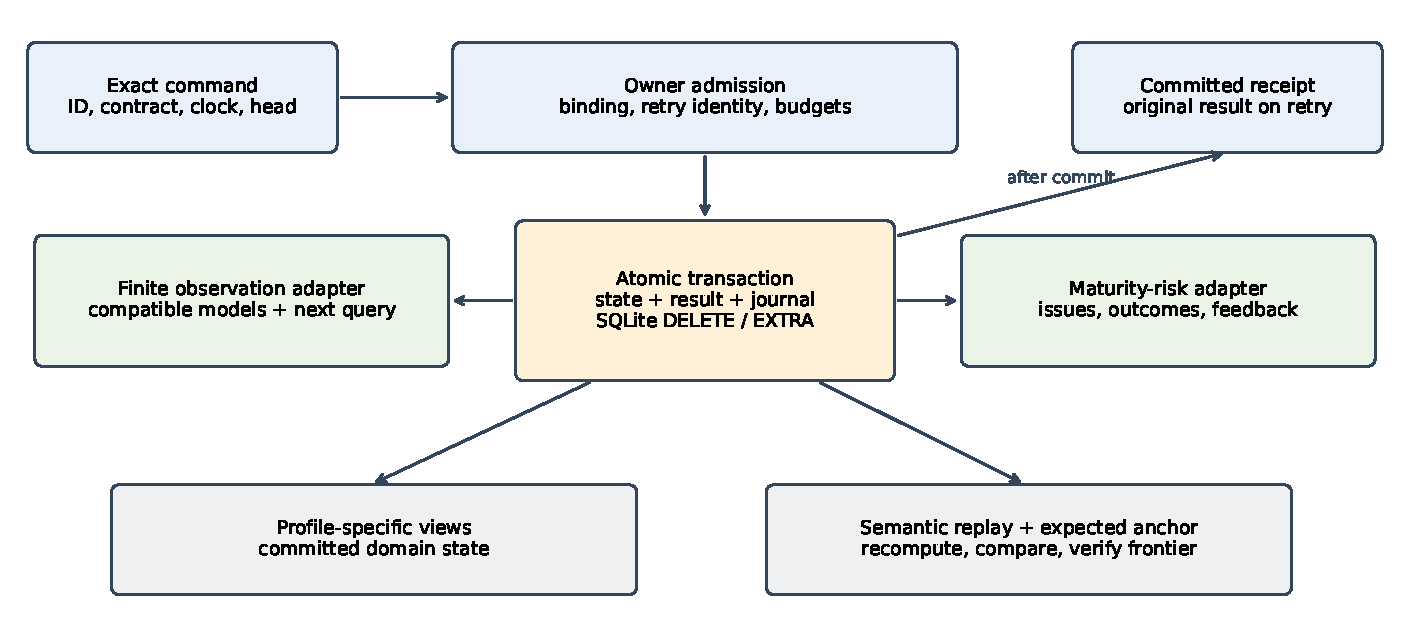
\includegraphics[width=\linewidth]{figures/runtime_architecture.pdf}
\caption{Shared operational composition. Commands bind immutable contracts and invoke one domain reducer. State, result and journal commit together; views expose committed domain semantics. Semantic replay uses the same declared adapters, while direct component comparisons and fault tests provide separate implementation checks.}\label{fig:runtimearchitecture}
\end{figure}

\subsection{Bounded reference scope}
The default limits permit at most 10000 unique committed commands, 10000000 canonical command bytes and 65536 bytes per command. They bound accepted logical input, not elapsed runtime, database size, replay work or denial-of-service resistance. The adapters rebuild retained domain histories, so per-command work grows with history and cumulative work can be quadratic or worse when combined with domain planning. The finite planner also retains its existing combinatorial scaling. A full semantic audit re-executes reducers and is distinct from an independently implemented mathematical verifier.

These two adapters retain their separate domain semantics. Section~\ref{sec:stream} adds a composed forecasting adapter. Other numerical modules remain available in the complete research project with their own implementation interfaces. High-rate acquisition, a physical XR adapter, distributed execution, external actuation and production storage qualification require additional implementation and validation.

\section{Forecast generation and correction-aware learning from received records}\label{sec:stream}
A forecast service must generate its predictions from available observations, retain what it actually issued and distinguish later corrections from information present at issuance. The composed stream adapter implements these three obligations under one transaction. It joins the existing volatility filters, eight-expert bank, transformed forecast aggregation and a bounded exposure proposal. The shared owner remains domain independent; this adapter is a specific positive-scalar risk profile.

\subsection{Three clocks and an immutable issuance record}
A source record contains observation index $i$, event time $t_i$, declared receipt time $r_i$, revision number and a positive finite value $x_i$. The owner ingests it at $\tau_i$, with $t_i\leq r_i\leq\tau_i$. New indexes are contiguous and their event times strictly increase. Revisions preserve the index and event time and advance the revision number. The horizon $h\in\{1,5\}$ counts observations: the target of an issue at index $i$ is index $i+h$. That unreceived observation's event time is not inferred by adding $h$ to a physical timestamp. If the current origin itself arrives late, the target event may already have occurred outside the store. The output therefore declares its basis as the next unreceived observation; after maturity it records whether the target event time actually exceeded issue time. Prefix nonanticipation does not by itself establish prediction before physical target occurrence.

On accepting a new source index, the adapter first makes eligible outstanding targets mature, reconstructs current feedback state and then attempts a forecast at the new origin. A correction updates the current information set without issuing a new forecast at an old origin. First maturity records the owner operation at which the required endpoint becomes available in this store; an earlier declared receipt alone cannot establish earlier ingestion. Missing future endpoints remain pending. The profile admits late receipts and revisions but requires new source indexes in order; buffering arbitrary out-of-order new indexes is outside its implemented contract.

Every emitted record retains the origin and target indexes, source-prefix identity, issue time, expert bank, mixture weights, gradient accumulator at issue, severity state, forecast and proposal. Its identity is immutable. Thus the prediction evaluated after a correction is the one actually issued. Re-running the entire forecasting procedure on revised history would instead construct a different hypothetical issuance history. The adapter uses that revised prefix for the next base forecast, while retaining the original banks and predictions for feedback on earlier issues.

\subsection{An explicit observation-to-forecast transition}
The base generator is unchanged: initialization from 60 one-observation losses, variance half-lives 20 and 120, a 250-scenario window and confidence $39/40$. Raw historical simulation and the five declared fast/slow variance mixtures supply six experts. Two further experts retain the fast quantile and apply the severity ratios with half-lives 125 and 500, initial ratio $1.5$ and emitted-ratio cap 20. All these half-lives count their respective observations or feedback updates, as specified in the preceding models. The raw severity accumulators are not clipped.

The first possible forecast origin is $60+h+250-1$ with zero-based indexing, requiring 311 observations for $h=1$ or 315 for $h=5$. The eight transformed forecasts are mixed with the current lane weights, using the existing cumulative gradient normalization at $c=0.1$. Each lane starts uniformly with zero accumulated squared norm at the first eligible part of the supplied stream. This is an explicit initialization convention; it does not reconstruct an omitted historical training interval.

For each mature issue $j$, the current source revisions determine
\begin{equation}
 Y_j=100\log\frac{x_{i_j+h}}{x_{i_j}}.
 \label{eq:streamloss}
\end{equation}
The unchanged fast quantile stored at issue determines the severity response. The unchanged expert bank and weights stored at issue determine the aggregate gradient. These contributions are folded in first-maturity order to reconstruct current severity and lane states. A revision replaces affected contributions and repeats this fold. One target supplies one active contribution; replaying a correction does not create a second target.

During warmup, or when a zero-variance or nonpositive-tail model cannot supply the required positive ordered bank, the adapter retains valid observations and explicitly reports forecast unavailability. It does not manufacture a positive forecast by clipping. Nonfinite derived arithmetic rejects the transition atomically. All floating results carry their binary64 status. The reference limits are 1024 source indexes, 2048 accepted source records including revisions, and 512 issues per contract. These are bounded execution limits rather than a streaming-throughput guarantee.

\subsection{A score bound that accounts for revised replay states}
Correction-aware feedback introduces a distinction absent from the regular uncorrected lane schedule. Let $u_j$ be the immutable weight vector originally used for issue $j$ and $v_j$ the state immediately before its update in the current replay. They can differ after a correction. A gradient evaluated at $u_j$ cannot be analyzed as though it had been evaluated at $v_j$.

Fix one lane and one finite as-of replay. Its original expert forecasts have $0<Q_{jk}\leq E_{jk}<\infty$, and its currently selected losses are finite. Put $a_{jk}=Q_{jk}/E_{jk}$, $b_{jk}=1/E_{jk}$. The convex score on the closed simplex is
\begin{equation}
 f_j(w)=-\log(b_j^\top w)+a_j^\top w+
     \frac{(Y_jb_j^\top w-a_j^\top w)_+}{\beta}-1,
 \qquad \beta=1/40.
 \label{eq:streamscore}
\end{equation}
The positive expert shortfalls ensure $b_j^\top w>0$ at every simplex point, including vertices. Choose a subgradient $g_j\in\partial f_j(u_j)$, using the zero hinge subgradient at equality, and center it:
\begin{equation}
 \bar g_j=g_j-\frac{\boldsymbol{1}^\top g_j}{K}\boldsymbol{1},\quad
 G_j=G_{j-1}+\norm{\bar g_j}_2^2,\quad
 v_{j+1}=\Pi_\Delta(v_j-\eta_j\bar g_j),\quad
 \eta_j=\frac{c}{\sqrt{G_j}}.
 \label{eq:streamreplay}
\end{equation}
Here $G_0=0$ and $c>0$. A zero-gradient round leaves $v$ unchanged; rounds before the first nonzero gradient use no positive step. The adapter uses $c=0.1$.

\begin{proposition}[Fixed-replay score comparison]\label{prop:streamregret}
In exact arithmetic, for any fixed comparator $w\in\Delta_K$ and the replay above,
\begin{equation}
 \sum_{j=1}^n\bigl(f_j(u_j)-f_j(w)\bigr)
 \leq (c+c^{-1})\sqrt{G_n}+\mathcal{M}_n,
 \qquad
 \mathcal{M}_n=\sum_{j=1}^n\bar g_j^\top(u_j-v_j).
 \label{eq:streambound}
\end{equation}
When $G_n=0$, the first term and $\mathcal{M}_n$ are zero and the left side is nonpositive. The result applies separately to each lane and may be summed over lanes with one fixed comparator per lane.
\end{proposition}
\begin{proof}
Convexity and centering give
\[
 f_j(u_j)-f_j(w)\leq
 \bar g_j^\top(v_j-w)+\bar g_j^\top(u_j-v_j).
\]
For a nonzero-gradient update, the projection inequality yields
\[
 \bar g_j^\top(v_j-w)\leq
 \frac{\norm{v_j-w}_2^2-\norm{v_{j+1}-w}_2^2}{2\eta_j}
 +\frac{\eta_j}{2}\norm{\bar g_j}_2^2.
\]
The simplex has squared diameter at most two and the positive step sizes are nonincreasing. Summing over nonzero-gradient rounds therefore bounds the distance terms by $1/\eta_n=\sqrt{G_n}/c$, where the final step means the last such round. Also
\[
 \sum_j\frac{G_j-G_{j-1}}{\sqrt{G_j}}\leq2\sqrt{G_n},
\]
so the remaining quadratic term is at most $c\sqrt{G_n}$. Zero centered gradients have zero tangent inner products and nonpositive score excess by convexity. Adding the explicit mismatch terms proves the claim.
\end{proof}

This is a specialization of the established projected-gradient argument \cite{zinkevich2003online}, with the evaluation-point mismatch retained. Delayed-feedback learning likewise requires a scheduling assumption matched to the update rule \cite{joulani2013delayed}. On the uncorrected sequential schedule, a lane's preceding target matures before its next issue and $u_j=v_j$, recovering the earlier bound. Following revisions, $\mathcal{M}_n$ is a signed correction term. The conservative upper bound $\sum_j\norm{\bar g_j}_2\norm{u_j-v_j}_2$ is available when only magnitudes are wanted. Neither term is assumed sublinear.

An explicit example shows why the correction cannot generally be discarded. Take two experts with $(Q_1,Q_2)=(1/2,1/4)$, $(E_1,E_2)=(1,1/2)$ and outcome zero in every round. Then $f(w)=-\log(w_1+2w_2)-1/2$. Evaluate every gradient at the stale issue vector $u_j=(1,0)$, while replay starts uniformly and updates by \eqref{eq:streamreplay}. The centered gradient is always $(1/2,-1/2)$. For $n=200$, $c=0.1$ and comparator $(0,1)$, the score excess is $200\log2>138$, whereas the bound without $\mathcal{M}_n$ is only $101$. This constructed stale-evaluation sequence is a mathematical counterexample to that omission, not a claim about a generated market trajectory.

The comparison fixes the issued banks and one selected revision of their outcomes. It does not compare with an alternative adaptive forecasting system whose different earlier decisions would generate different banks. Replacing a source revision changes the compared functions and requires another replay. The mathematical statement is in exact arithmetic; binary64 execution checks supply numerical evidence with stated tolerances.

\subsection{A maximal proposal under an explicit model budget}
For an emitted shortfall $E>0$, let $\widehat E$ be the exact dyadic rational represented by its stored binary64 value. A bound contract specifies a nonnegative rational budget $B$, positive rational exposure per unit $\delta$ and integer cap $N$. Its proposal is
\begin{equation}
 k^*=\min\left(N,\left\lfloor\frac{100B}{\delta\widehat E}\right\rfloor\right),
 \qquad X^*=\delta k^*.
 \label{eq:streamproposal}
\end{equation}
This is the largest integer quantity in $[0,N]$ satisfying the declared proxy constraint $\delta k\widehat E/100\leq B$. Division and comparison use rational arithmetic, so maximality follows directly from the defining floor inequality. The retained proposal includes the chosen and next-unit proxy values, making the boundary independently checkable.

This calculation limits a model-derived log-loss proxy for one proposal. It does not bound realized losses, certify the estimated shortfall, convert logarithmic losses into exact monetary P\&L or reserve capacity across several outstanding proposals. The output is read-only. Actual holdings, cumulative capital allocation and external execution require additional state and a separate validated application contract.

\section{Incremental execution with preserved forecast semantics}\label{sec:incremental}
The stream profile in Section~\ref{sec:stream} defines which outputs are justified by each received prefix. Its direct implementation repeatedly reconstructs the same variance and feedback histories and computes historical forecast rows that are then discarded. These computations can be reduced without selecting a new predictive model. The target is observational equivalence: the same accepted observations must produce the same domain states, issued records, proposals and views.

Dependency tracking, memoization and consistency with fresh evaluation are established ideas in incremental computation \cite{acar2013consistent}. Here they are specialized to immutable issued forecasts and corrected endpoint observations. The contribution is a concrete dependency structure, a bounded implementation and an executed comparison with the retained full-replay reference. The implementation is not a general self-adjusting language or a machine-checked semantics.

\subsection{Dependencies of a corrected observation}
Let $x_s>0$ be the currently selected source value at index $s$. One-interval losses and horizon-$h$ losses are
\[
 r_t=100\log(x_t/x_{t-1}),\qquad
 y_t^{(h)}=100\log(x_t/x_{t-h}).
\]
Changing only $x_s$ can change $r_s,r_{s+1}$ and $y_s^{(h)},y_{s+h}^{(h)}$, when those indexes exist. Other raw endpoint losses are unchanged. This locality does not imply local forecast dependence: a variance recurrence propagates the changed input through its subsequent state.

For each decay $\lambda$, the reference variance has a seed at index $b=60$ and a sequential update,
\begin{equation}
 V_b=\frac1b\sum_{t=1}^{b}r_t^2,\qquad
 V_t=\lambda V_{t-1}+(1-\lambda)r_t^2,\quad t>b.
 \label{eq:incrementalvariance}
\end{equation}
If a changed return enters the seed, the seed reduction and its dependent suffix must be recomputed. Otherwise, retain the variance prefix strictly before the first changed recurrence input and replay its suffix in the original order. An old correction outside the current scenario window can still change its standardizing variances and the current forecast. Keeping only the most recent 250 raw prices would therefore not preserve the reference calculation. The reference's positive-variance guard also covers the complete retained variance history. Its finite-scenario checks cover the union of all eligible historical rows. Reducing only the current row must retain this global acceptance condition, even when an older nonfinite scenario has left the current window.

A completed forecast with origin $i$ uses only $x_i,x_{i+h}$ for its current outcome. Consequently, a correction at $s$ can change the numerical feedback contribution of at most two issued forecasts: origins $s$ and $s-h$. Both belong to lane $s\bmod h$. Their gradients depend on their immutable issued banks and weights, not on the newly reconstructed learner weights. Unchanged gradient contributions can therefore be reused even when the weights to which they are applied change.

\begin{proposition}[Correction locality]\label{prop:incrementallocality}
Fix a horizon, a valid issuance history, its first-maturity order and a correction to one existing source index. Hold the issued banks, issued weights and target identities fixed. Apart from at most two mature contributions in the corrected index's lane, all numerical outcome gradients and severity responses are unchanged. The reconstructed aggregation states in other lanes are unchanged. In the affected lane, an exact update is obtained by retaining the state before its first changed contribution and replaying all subsequent updates in that lane. The two global severity recurrences may require replay from the earliest changed contribution across the complete maturity order.
\end{proposition}
\begin{proof}
An issued outcome reads precisely its two endpoints. Solving $s=i$ or $s=i+h$ gives the two possible origins, whose residues modulo $h$ agree. Each gradient is a deterministic function of that outcome and the fixed issued bank and weights. Its norm and severity response inherit the same dependencies. Aggregation updates read only their own lane's preceding weights and accumulated gradient energy. Induction along every unaffected lane therefore preserves all its states. The same induction preserves the affected lane's prefix and determines its recomputed suffix. Severity uses one shared ordered recurrence for each decay, so a changed response can affect all its subsequent states, including responses from other lanes.
\end{proof}
A revision that changes provenance but leaves the binary64 source value unchanged need not change any numerical contribution. Its accepted source record and the provenance of a subsequent issue still change. Numerical reuse never substitutes an earlier provenance record for the current one.

\subsection{Disposable caches and observable state}
The optimized execution profile leaves the original transition, validation, issuance and serialization contracts intact. Its caches contain derived numerical work and checkpoints. They are not persisted as independent source evidence. Cache clearing or eviction changes the amount of work, not the domain state. Reopening a store reconstructs execution from the retained commands under an explicitly selected implementation binding.

Reuse requires the actual inputs of a computation to agree, including every relevant issued field and the preceding recurrence state. A stored digest is not sufficient if the object whose digest it purports to identify has changed. Configurations, rewound histories and interleaved contracts must also be distinguished. A failed candidate transition may have performed cache work; subsequent accepted transitions still have to match their own dependencies. Correctness cannot rely on the last attempted command having committed.

\begin{proposition}[A sufficient cache-refinement condition]\label{prop:incrementalrefinement}
Let a successful reference transition have a finite acyclic evaluation of deterministic primitives, with explicit source inputs and an ordered recurrence unrolled into that evaluation. Suppose an alternative evaluator follows the same branch guards and demanded computations, retains completed cached values immutably, and (i) reuses a node only when all its primitive inputs and its primitive identity equal those of a completed earlier evaluation, (ii) recomputes every other needed node using the same primitive, and (iii) constructs observable records from the current source inputs and resulting node values. Then its observable result equals fresh reference evaluation. Clearing any subset of cached nodes preserves this equality.
\end{proposition}
\begin{proof}
Order the required nodes topologically. Source nodes have the current reference values. At each subsequent node, the induction hypothesis gives the same predecessor values as fresh evaluation. A reused value was computed by the same deterministic primitive on these inputs; a recomputed value is obtained by that primitive now. Both equal the fresh value. Induction reaches every observable output. Removing a cache entry changes a reuse into a recomputation and leaves the argument unchanged.
\end{proof}
This criterion applies to exact-real evaluation and to fixed deterministic machine primitives. Bitwise equivalence additionally requires exact typed machine inputs and preservation of the machine operations and reductions, rather than algebraic equivalence alone. In particular, replacing a sequential severity fold by an affine correction formula can change binary64 rounding. The implementation retains sequential recurrence operations and is compared byte for byte with the reference in the recorded numerical environment. Rejected inputs and arithmetic failures are tested separately against the reference. The evaluator must retain its short-circuit rules: evaluating an otherwise unused expression that overflows could change acceptance. The proposition does not supply a formal verification of Python, NumPy or the hardware.

For current forecast generation, only the final eligible origin is needed. Each empirical quantile and tail-mean calculation reads its own scenario row; previous origins contribute no input to that row. The optimized evaluator constructs the current raw and five standardized rows and retains the original within-row reductions. The full reference remains independently executable. Exact state and result equality is the comparison target; owner journal hashes differ between execution profiles because their headers bind different implementations.

\subsection{Numerical work and retained materialization costs}
Write $W$ for the scenario-window length, $K$ for the expert count and $m$ for completed issued targets. With a warm compatible cache and no correction, an appended observation requires one new variance recurrence step per decay, at most one new mature gradient and lane update, and one current row for each of the six base experts. A complete view still exposes the existing feedback records.

Across $p$ successful forecast origins, the direct forecaster evaluates $6p(p+1)/2$ scenario rows when every eligible origin emits; evaluating only the current origin requires $6p$. Similarly, replaying $m$ completed contributions after each new completion requires $m(m+1)/2$ gradient evaluations, whereas a compatible incremental history needs $m$. These are operation counts for the stipulated execution pattern, not wall-clock bounds for the complete runtime. Warmup, unavailable forecasts, explicit views, cache misses and corrections are counted separately in the experiment.

A correction may invalidate a long variance or recurrence suffix. Even when it changes only two gradients, many subsequent projections or severity steps can require replay. The optimized forecaster still constructs full-prefix horizon returns, mixed variances and standardized arrays; these numerical array operations remain linear in retained source length. The public state and view also retain histories whose size grows with the accepted prefix. Dependency comparison, canonical copying, hashing, result materialization and durable journaling therefore remain history-dependent. This implementation neither has constant end-to-end update cost nor establishes high-throughput or real-time deployment. Its measurable claim is reduced repeated numerical work with preserved outputs under the specified capacity and environment.

\section{Reducing materialization cost under an unchanged transaction contract}\label{sec:fastowner}
Numerical reuse leaves an independent cost in the operational owner: copying, validating, encoding and hashing the retained state. A domain-independent execution alternative reduces these repeated traversals. It uses the same adapters, accepted commands, SQLite format and single-command commit boundary as Section~\ref{sec:runtime}. No numerical recurrence or forecasting policy is changed. The contribution is an explicit preservation argument and an executed implementation comparison, rather than a new serialization or transaction protocol.

\subsection{An order-preserving structural copy}
Let $\mathcal J$ contain the exact interchange values accepted by the owner: null, Boolean values, integers of magnitude at most $2^{53}-1$, ASCII strings, lists and dictionaries with ASCII string keys. Containers must have the exact declared Python type, and the maximum permitted depth is 64, counting the root at zero. Floating-point quantities use the existing typed string encodings. Let $C(x)$ be the owner's sorted-key compact ASCII JSON representation and let $L$ be its strict decoder. The reference copy is
\[
 R(x)=L(C(x)).
\]
In this implementation, $L$ also validates its result through $C$, so each reference copy performs two validation/encoding passes and one parse. The structural alternative $T$ validates scalar types and bounds directly, copies list elements recursively, and reconstructs each dictionary in sorted-key order. Sorting is essential: an adapter may observe dictionary iteration order even when all persisted JSON is canonical. The standard encoder's key-sorting option and decoder hooks supply the relevant ordering and parsing interfaces \cite{pythonjson312}; the stricter interchange domain is imposed by Gabriel.

\begin{proposition}[Preservation of the interchange copy]\label{prop:typedcopy}
For every $x\in\mathcal J$, $T(x)$ and $R(x)$ have equal scalar values, container types, list order and dictionary iteration order. Both expand repeated mutable references into separate subtrees, and neither shares a mutable container with $x$. The structural procedure rejects types, characters, integer magnitudes and depths outside the same specified domain.
\end{proposition}
\begin{proof}
For each permitted scalar type, encoding and decoding recover its value and exact type; the structural procedure returns that immutable value. For lists, both procedures preserve element order and independently visit every occurrence. Applying the induction hypothesis to each child gives equal contents and fresh containers, including when two children originally refer to the same container. For dictionaries, canonical encoding orders keys lexicographically, decoding inserts them in that order, and the structural procedure uses the same order. Applying the induction hypothesis to the associated values completes the argument. The common type, character, magnitude and depth predicates give the domain restriction. A cycle necessarily exceeds the finite depth bound on a traversal and is rejected. This statement concerns the declared data semantics, not object addresses or the identity of immutable scalar objects.
\end{proof}

\subsection{Canonical text as a local reusable result}
A stored state is still decoded and checked against its canonical re-encoding before use. Within the transaction, its validated text supplies the pre-state digest directly. After a reducer returns a checked, detached state, one canonical representation supplies both its post-state digest and its SQL value. The text is computed or validated locally; an adapter cannot supply a trusted hash in its place. No state or validation cache survives an owner call. Thus another writer or modified stored row cannot be hidden by an earlier cache entry.

The implementation retains strict parsing, registry validation, the compare-and-set journal head, command identity, receipt-time ordering and all input budgets. Identical retries return the original receipt without a new journal event. A fresh opening still replays the entire journal. Each unique command still uses one \texttt{BEGIN IMMEDIATE} transaction, rollback-journal \texttt{DELETE} mode and \texttt{synchronous=EXTRA}; the interpretation of these guarantees follows SQLite's documented storage assumptions \cite{sqliteatomic,sqlitepragmas}.

\begin{proposition}[Owner execution equivalence]\label{prop:ownerequivalence}
Consider the reference and structural-copy owners on identical valid database states and the same ordered commands. Suppose the registered adapters obey the local deterministic data contract: their outputs depend on the supplied values and container order, not on object identity, interning, allocation behavior, wall time or external side effects. Assume stable inputs, adequate resources and normal database execution. With the same numerical environment, the owners accept the same commands and produce equal canonical receipts, journal rows, contract states and accounting. Rejected transitions leave the same committed database state. Both owners give the same semantic-audit acceptance or rejection for a produced store under the same registry.
\end{proposition}
\begin{proof}
The command parser, metadata checks, retry branch and admission predicates are unchanged. For a new transition, Proposition~\ref{prop:typedcopy} gives adapters equivalent detached arguments and gives equal checked outputs. If $t$ is validated canonical stored state text, then $t=C(L(t))$; hashing $t$ therefore equals recomputing and hashing the state's canonical representation. The new post-state text is exactly $C(s')$ and is used unchanged for both hashing and storage. Every field of the journal record and receipt is consequently equal, giving equal canonical bytes and head identifiers. The same SQL operations and transaction boundary commit them together. On an exception, both roll back. Induction over accepted commands proves the claim; duplicate commands do not advance the induction state. The inherited semantic audit uses the same transition construction and compares the entire reconstructed record and final database state, so the argument applies across owner implementations as well.
\end{proof}

This is a source-level refinement argument, supported by differential and fault tests. It is not a machine-checked proof of Python, SQLite, the adapters or physical power-loss durability. Exception wording, allocation counts and elapsed time are not part of the preserved data contract. The alternative still traverses and persists complete retained states: it reduces repeated work without changing the history-dependent asymptotic storage or replay costs. Batching commits, shortening audits or changing synchronization would define different comparisons and are not used here.

\subsection{An auxiliary native kernel for bounded graph signatures}\label{sec:packedgraph}
The same separation of mathematical output from execution work applies to a bounded graph-analysis component. The optional native implementation specializes the signature path in the supplied PSE software \cite{psearchive}. It accepts a simple undirected binary graph on $1\leq n\leq7$ vertices and preserves the existing signature convention: embed the graph into the fixed zero-padded $13\times13$ matrix, act on seven available vertex slots by $S_7$, and select the lexicographically least row-major matrix. The remaining signature fields include the original vertex and edge counts, orbit and stabilizer sizes, spectral summaries and fixed subgraph indicators. This is an auxiliary analysis kernel; it is not invoked by the financial reducers or the transactional owner.

There are 21 potential edges among the seven slots. Store their occupancy in a 21-bit word and precompute the edge permutation induced by every $\pi\in S_7$. For the comparison key, put upper-triangle entries in row-major order, with the earliest entry as the most significant bit. Minimizing an arbitrary packed integer would generally give a different canonical convention.

\begin{proposition}[Preservation of the padded graph orbit]\label{prop:packedorbit}
For a simple undirected binary graph in the stated range, permutation of its 21 edge bits yields exactly the padded matrix orbit under $S_7$. The minimum row-major comparison key reconstructs the same canonical matrix as dense conjugation. Counting permutations that fix the input gives its stabilizer size, and the orbit size is $7!$ divided by that count.
\end{proposition}
\begin{proof}
Each permutation maps an unordered vertex pair to an unordered vertex pair, so its action on edge occupancy equals a permutation-matrix conjugation of adjacency. The two indexing conventions may invert the permutation; inversion is a bijection of $S_7$ and leaves the orbit and stabilizer count unchanged. Entries outside the seven active slots and diagonal entries are fixed. For two distinct symmetric adjacency matrices, the first differing row-major entry must be in the upper triangle: any differing lower-triangle entry repeats an earlier upper-triangle difference. Thus the specified integer ordering and full matrix ordering have the same minimum. Enumeration covers all elements of $S_7$ once, and the orbit--stabilizer identity gives the stated cardinality.
\end{proof}

The inherited conjugation routine loops over four matrix indices, evaluating $13^4$ summands for each permutation even though a permutation matrix has only one nonzero per row. Its full scan repeats orbit work for several report fields. The optimized path operates on occupied edge bits and avoids constructing dense orbit matrices and report fields discarded by the signature consumer. Spectral and subgraph routines still operate on the original embedding, through the original floating-point functions; a merely isomorphic reordered matrix need not preserve numerical bytes. Ineligible regions return before permutation-cache initialization. This reduces execution work for the bounded operation, without asserting a new canonical-labeling method.

The preserved legacy hash omits $n$ from its padded representation. For example, edgeless one- and two-vertex graphs have the same padded matrix and hash although their complete signatures differ in $n$. The hash alone is therefore unsuitable as an exact identity for variable-size records. More generally, neither unlabeled graph equivalence nor a spectral descriptor proves equality of node data, future dynamics or a decision. No such shortcut is admitted into the owner equivalence of Proposition~\ref{prop:ownerequivalence}.

\subsection{Full replay by direct expected-byte comparison}\label{sec:replayowner}
Complete semantic replay need not parse every stored derived output. It must reconstruct and compare those outputs. The replay owner retains independent strict parsing of each command and recomputes every adapter transition. For a reconstructed value $y$ and stored text $s$, it compares
\begin{equation}\label{eq:expectedbytes}
 s=C(y).
\end{equation}
The reference first requires that $s$ decode into the interchange domain, then checks $C(L(s))=s$ and $C(L(s))=C(y)$. Equation~\eqref{eq:expectedbytes} combines these requirements because $C(y)$ is itself valid canonical text. Consequently, duplicate keys, alternative numeric types, whitespace, reordered keys, alternative escaping and non-JSON storage values cannot pass merely by decoding to a similar object.

\begin{proposition}[Preservation of full replay acceptance]\label{prop:replayaudit}
Under the deterministic value-based adapter assumptions of Proposition~\ref{prop:ownerequivalence}, consider databases with the declared schema and fixed stored field values. Replace the reference's parsing and canonical comparison of derived records, receipts and terminal contract states by direct comparison with their freshly regenerated canonical text. Retain independent command parsing, all admission and registry checks, metadata and external-anchor checks, and validation of the complete terminal bindings object. Under normal database execution and adequate resources, the two audits accept the same databases and return the same audit result.
\end{proposition}
\begin{proof}
For any regenerated interchange value $y$, the reference's two text equalities hold if and only if $s=C(y)$. If the direct equality holds, the stored value necessarily has the exact syntax and data-domain properties of $C(y)$; strict decoding succeeds and recovers $y$. Conversely, acceptance of the reference equalities implies the direct equality. Starting from the independently checked header, induction over the ordered commands gives the same regenerated binding, record, receipt and head at each step, by Proposition~\ref{prop:typedcopy}. Apply the text equivalence at every derived output and at the terminal states and configurations. Retaining the same complete-binding validation also preserves its aggregate depth constraint; independently valid states do not by themselves guarantee that this larger object is valid. Identical metadata and anchor predicates complete the acceptance equivalence.
\end{proof}

The implementation retains the latest freshly generated canonical state string for each bound contract during one audit. Its hash supplies the next pre-state digest. The string is never loaded as an authoritative checkpoint and is discarded with that audit. Stored records and receipts never supply the reconstructed state. A subsequent audit recomputes every transition again. The inherited admission rules can persist an individually valid deep state whose complete bindings object exceeds the aggregate audit limit; the refinement preserves this rejection rather than broadening the accepted domain. The implementation inherits live submissions, transaction boundaries, reads and exports from the structural-copy owner without overriding them. Error messages, rejection timing and allocation behavior may differ; accepted data and rejection of invalid stored values are the preserved contract. Adapter mathematics and hash authentication remain separate questions.

This refinement changes neither the number of journal events replayed nor the storage format. In histories retaining increasingly large outputs, complete reconstruction and comparison still require substantial work. It removes repeated decoding and canonicalization of derived stored objects without introducing a trusted summary of the prefix.

\subsection{A certified finite index for the bounded graph action}\label{sec:graphindex}
For seven slots, the graph domain $X=\{0,\ldots,2^{21}-1\}$ is small enough to tabulate its complete $S_7$ orbit partition. The generator assigns a class identifier $c(g)$ to each edge word $g$, a representative $r_k$ to each class $k$, and a permutation witness $w_g$. An independent checker verifies
\begin{equation}\label{eq:indexcertificate}
 g=w_g\mathbin{\cdot}r_{c(g)},\qquad
 c(\tau_i\mathbin{\cdot}g)=c(g)\quad(i=1,\ldots,6),
\end{equation}
where $\tau_i$ exchanges two adjacent vertex slots. The checker uses direct row and column permutations of adjacency matrices, separately from the generator's edge-permutation maps. It validates each witness as a bijection, each class identifier as an in-range integer, and each class as nonempty.

\begin{proposition}[Certificate for a complete finite orbit index]\label{prop:graphindex}
If the stated checks hold for every $g\in X$, the fibers of $c$ are exactly the $S_7$ orbits. Let $a_k\in X$ be the member of fiber $k$ with the least row-major comparison key, and let $m_k$ be the number of its members. Then
\[
 (a_{c(g)},m_{c(g)},7!/m_{c(g)})
\]
is the canonical edge word, orbit size and stabilizer order of $g$ under the convention of Proposition~\ref{prop:packedorbit}.
\end{proposition}
\begin{proof}
The witness equation puts every member of a fiber in the orbit of its representative, so a fiber cannot merge distinct orbits. The six adjacent transpositions generate $S_7$. Closure under these generators puts the entire orbit of any member into its fiber, so no orbit is split between fibers. Nonemptiness therefore makes each fiber exactly one orbit. Taking the minimum in the specified row-major order gives its canonical edge word. Counting all fiber members gives its orbit size, and the orbit--stabilizer identity gives $7!/m_k$.
\end{proof}

The certificate distinguishes correctness of a table from byte-for-byte reproduction of one generator run. A different valid witness for the same graph must be accepted. The checker also independently recomputes each fiber's cardinality and minimum and compares the stored metadata. The value $a_k$ is an edge word, not the integer comparison key; confusing these two orderings would change the legacy canonical matrix.

The generated index contains 1,044 classes. A two-byte class identifier for every graph and a 16-byte metadata row for every class occupy 4,211,008 bytes. Four-byte witnesses occupy another 8,388,608 bytes for offline verification and are not needed for lookup. A lookup retrieves an orbit triple in constant indexed work after the input edge word is formed. This is finite precomputation with an explicit verification contract, not a general improvement in graph-isomorphism complexity: the occupancy domain grows as $2^{n(n-1)/2}$.

The finite table certificate establishes the integer orbit data. An integration preserving the complete signature must additionally retain input validation and the spectral and subgraph routines on the original embedding. Those floating-point outputs are not reconstructed by the table certificate.

\subsection{Exact-input reuse of complete graph signatures}\label{sec:signaturecache}
The finite index replaces the orbit calculation, while the remaining signature fields still require evaluation. Repeated labelled inputs permit a separate refinement: retain a completed signature and reuse it only for the identical matrix. This refinement does not identify isomorphic matrices or replace the spectral routines.

Let $F(A)$ denote the complete indexed signature of an adjacency matrix $A$, including its original dimension. Hold the executable, numerical libraries and floating-point environment fixed, and assume that $F$ is deterministic at the level of every returned field's representation. Ordinary validation and the restriction $1\leq n\leq7$ precede every cache lookup. The cache domain $D$ consists of the accepted matrices whose \emph{entire} $n\times n$ array contains only the exact binary64 encodings of $+0.0$ and $1.0$. Define
\[
 K(A)=\left(n,\sum_{0\leq i<j<n} A_{ij}\,2^{j(j-1)/2+i}\right),\qquad A\in D.
\]
The sum here denotes integer packing of the zero--one entries. Numerical validation also admits $-0.0$; any such encoding, including one on the diagonal or below it, bypasses the cache and invokes $F$ unchanged.

\begin{proposition}[Preservation by exact-input signature reuse]\label{prop:signaturecache}
Under the stated determinism assumptions and adequate execution resources, consider any finite sequence of signature calls and cache resets on a thread. A cache initially empty, or populated only by earlier calls satisfying this contract, stores completed values of $F$, compares the full key $K$ before reuse, and returns independent owned copies. Misses and bypasses invoke the unchanged calculation, and invalid inputs undergo the same validation before lookup. Then every successful call returns exactly the complete output of fresh evaluation on its own input, including the binary64 representation of every floating-point field. Arbitrary slot collisions, eviction, reset, and interleaving calls from new engine instances on that thread preserve this equality. A cache with 256 slots retains at most 256 entries on each thread.
\end{proposition}
\begin{proof}
The key is injective on $D$: its dimension and upper-triangle bits determine every upper-triangle entry; validated symmetry determines the lower triangle; and the validated diagonal consists of positive zeros. Restricting all entries to the two stated encodings makes this reconstruction exact as a binary64 array. Maintain the invariant that each occupied slot contains an owned copy of $F(A)$ for its stored key. On a matching hit, injectivity gives the same input array and determinism gives the same complete result. A miss computes that result directly and stores a copy, preserving the invariant even when another key is evicted. Bypasses compute directly without inserting; validation failures occur before lookup. Independent copies prevent callers from modifying retained values. Reset removes entries and therefore preserves the invariant. Induction over the finite sequence proves the assertion; a new engine instance changes neither the input-based key nor the invariant. The slot count supplies the entry bound.
\end{proof}

This is a preservation argument relative to $F$, not a proof of spectral accuracy, hash uniqueness or general engine equivalence. Relabelling can change floating-point results even when graph invariants agree mathematically. The key consequently contains the labelled edge word and dimension, rather than the orbit class or canonical hash. Each thread owns its cache; constructing a new engine on the same thread does not clear it. The stated bound counts retained entries per thread, not allocator bytes, process resident memory or entries across an unbounded number of threads. Lookup, validation and cloning still cost work, and the proposition supplies no speed guarantee. Reuse after a change in the floating-point environment is outside its assumptions.


\subsection{Call-local reuse in the spectral path}
\label{sec:spectralreuse}

Two optional transformations remove repeated computation within a committed
macrostep.  The \texttt{phase-hoist} feature reuses mode phases across ordered
vertex pairs in the continuous-time quantum-walk (CTQW) calculation.  The
\texttt{shared-spectrum} feature passes the eigensystem already constructed for
the C16 topological signature to the subsequent C18 multiscale calculation.
Neither transformation changes the eigensolver, the retained modes, the time
grid, the threshold, or the initial Kuramoto state used by C18.  These are
implementation refinements of the existing finite computation, not new
spectral approximations.

Let $n$ be the length of the first stored eigenvector, $k$ the stored truncation
rank, $S$ the number of scan steps, and $T$ the reporting time.  The reference
computes $\Delta t=T/S$ in binary64 arithmetic and evaluates
\[
 a_{jd}(t)=\sum_{m=0}^{k-1}
       \bigl(\cos(-\lambda_m t)+i\sin(-\lambda_m t)\bigr)u_{mj}u_{md},
 \qquad p_{jd}(t)=|a_{jd}(t)|^2.
\]
The displayed formula describes the expression; the implementation additionally
fixes its evaluation order.  Each real and imaginary term is multiplied
left-to-right and accumulated in increasing mode order.  An absent eigenvector
entry contributes the reference fallback value $+0$.  Missing eigenvalues are
not given such a fallback.  The first threshold crossing is stored for each
ordered pair, and the complete transfer matrix is evaluated separately at $T$.

\begin{proposition}[Conditional refinement by mode-phase reuse]
\label{prop:phasehoist}
Assume sufficient resources, $k\leq\lvert\lambda\rvert$ when $n>0$, and an
execution environment in which the employed scalar arithmetic and
trigonometric functions return the same bit pattern whenever given the same
operand bit patterns.  Preserve the reference multiplication and summation
orders, zero fallbacks, comparisons, and reporting calculation.  Replacing
repeated evaluations of $\cos(-\lambda_m t)$ and $\sin(-\lambda_m t)$ for a
given mode and time by stored results preserves every returned CTQW field
bit-for-bit.  The claim concerns returned data, excluding allocation behaviour,
execution time, and externally observable floating-point exception flags.
\end{proposition}

\begin{proof}
At any fixed scan step the phase operands are independent of the ordered
vertex pair.  Repeatability therefore makes each stored sine and cosine
identical to the value that the corresponding reference call would return.
For a fixed pair, induction over the mode index gives identical partial real
and imaginary sums, because neither the remaining operands nor their ordering
changes.  Consequently the probability and its threshold comparison agree.
Induction over scan steps then gives the same first-crossing table and the
same decisions to skip already resolved pairs.  The final matrix follows by
the same mode induction, using a freshly computed phase at the supplied $T$.
This separate evaluation is necessary: in floating-point arithmetic
$S(T/S)$ need not have the same bits as $T$.  The unchanged speed and mean-time
postprocessing receives identical inputs.  Empty first eigenvectors cause the
same early return in both implementations.  For $S=0$ the scan is empty and
the separate reporting calculation still applies.  For $k=0$ both mode sums
are empty.  These observations cover the respective boundary cases.
\end{proof}

Repeatability is an explicit implementation assumption, stronger than merely
specifying binary64 or fixing the rounding mode.  The Rust standard-library
contract does not promise a universally reproducible implementation of
\texttt{sin}/\texttt{cos}; NaN sign and payload propagation also lack a portable
bit-pattern guarantee \cite{rustf64docs}.  Bit comparisons involving nonfinite values therefore
document the pinned build and test inputs rather than establish a theorem over
all conforming Rust implementations.  Finite inputs that overflow into
nonfinite intermediates require the same qualification.  The transformation
does not certify the accuracy of the retained eigensystem, normalize a
truncated transfer matrix, or reinterpret the reference quantity $1/t_*$ as
a physical propagation velocity.

The implementation checks a conservative finite domain before entering the reused-phase path. On targets with at most 64-bit indices, it admits $k\leq2^{32}$, consumed eigenvector entries with magnitude at most $2^{128}$, and consumed eigenvalues and reporting times with magnitude at most $2^{250}$. A nonzero reporting time must have magnitude at least $2^{-250}$; both signed zeros are admitted. The threshold must be finite, the scan must have at least one step, and all consumed eigenvalues must exist. Other inputs delegate to the unchanged reference function, which is marked non-inlined in every compared build. The bounds are exact binary powers and deliberately conservative; they are sufficient implementation guards, not a characterization of all safe inputs.

Under ordinary round-to-nearest binary64 arithmetic and finite sine/cosine values of magnitude at most two, these bounds leave a large overflow margin: scan phases have magnitude below $2^{502}$, mode sums below $2^{293}$, and squared probabilities below $2^{588}$. Nonzero scan times remain large enough that reciprocals are finite. This guard avoids introducing a different NaN-producing arithmetic path for exceptional data. Delegation is also used for zero-step scans and malformed ranks, retaining reference returns or failures. The guard does not strengthen Rust's portable trigonometric contract; Proposition~\ref{prop:phasehoist} retains its explicit repeatability assumption. Checking the consumed arrays adds $O(k+kn)$ work in a dense representation.

The source-level work reduction can be stated independently of elapsed time.
Let $Q_s$ be the number of unresolved ordered pairs at scan step $s$.
For $n>0$ on an input admitted to the reused-phase path, the reference evaluates
\[
 N_{\rm trig}^{\rm reference}
   =2k\left(n^2+\sum_{s=1}^{S}Q_s\right)
\]
scalar trigonometric expressions, counting sine and cosine separately.  Let
$H=\#\{s:Q_s>0\}$.  The implemented lazy phase buffer is filled only at the
first unresolved pair of each step, giving
\[
 N_{\rm trig}^{\rm hoisted}=2k(H+1)
 \leq N_{\rm trig}^{\rm reference}.
\]
The inequality follows from $H\leq\sum_s Q_s$ and $1\leq n^2$.  The
additional buffers contain $2k$
binary64 values, or $16k$ payload bytes, plus their vector metadata and any
allocator overhead.  Pairwise products and accumulation remain proportional
to $k(n^2+\sum_s Q_s)$; phase reuse does not remove this work or the returned
$n\times n$ matrices.  These are source-level counts, not guaranteed emitted
machine-instruction counts or speedup estimates.  Lazy initialization avoids
phase evaluations after all pairs are resolved; outside the admitted domain the reference cost remains. With $n=1$, both functions
evaluate only the final reporting phase.  Buffer allocation and lookup costs
still prevent a universal wall-clock speedup claim.

\begin{proposition}[Reuse of an unchanged within-step eigensystem]
\label{prop:sharedspectrum}
Suppose C16 and C18 observe the same persistent graph and node order, use the
same effective spectral rank, and the Laplacian construction and eigensolver
are repeatable under the selected implementation.  Retaining the C16
eigensystem and moving it to C18 preserves the spectral input of C18
bit-for-bit relative to recomputation.  If every other input and branch
decision is unchanged, the resulting multiscale output is unchanged as well.
\end{proposition}

\begin{proof}
The reference C16 path constructs the Laplacian of the graph and calls the
eigensolver with $\min(k_{\max},n)$.  The reference C18 path constructs the
same Laplacian and supplies $k_{\max}$; the eigensolver applies the same minimum
internally.  The special $n=0$ and $n=1$ branches also return the same values.
The two computations thus have identical effective inputs and, by
repeatability, identical outputs.  C16 only reads its eigensystem while
constructing the topological signature.  Moving this value into C18 replaces
the second computation by its identical result.  No graph mutation intervenes.
C18 independently initializes its Kuramoto state exactly as before: it does
not inherit the state advanced by C16.  The remaining conditional assertion
follows by substitution into the unchanged multiscale calculation.
\end{proof}

In the implemented path the reuse applies when $n\leq500$.  For larger graphs
C16 retains its existing size-based fallback and C18 remains skipped.  The
retained eigensystem is local to one macrostep and is transferred without a
deep clone; there is no lookup key or cross-step invalidation problem.  The
transformation removes one Laplacian construction and one eigendecomposition
per eligible committed macrostep.  It extends the lifetime of the C16 result
until C18 consumes it and removes the second set of construction temporaries;
an allocator-independent peak-memory reduction is not asserted.

Full-engine equivalence has a further boundary.  The existing multiscale code
contains wall-clock budget branches, so faster arithmetic alone cannot imply
identical output under every operating-system schedule.  The conditional
branch assumption in Proposition~\ref{prop:sharedspectrum} makes this boundary
explicit.  Tests comparing selected state and complete crystal bytes establish
equality for the executed inputs and observed branch outcomes; they neither
eliminate these timing dependencies nor repair previously identified
mathematical limitations of the inherited spectral and clustering routines.

\subsection{Conditioned state queries on recognized weighted cliques}
\label{sec:conditionedwalk}
A continuous-time quantum walk uses unitary state evolution generated by a
Hermitian graph operator \cite{farhigutmann1998}. The auxiliary interface here
returns the complete complex state $\psi(t)=\exp(-itL)\psi_0$ for a specified
source $\psi_0$, fixed real symmetric $L$, and dimensionless time $t$. It is
separately invoked and does not change the all-pairs threshold statistic of
Section~\ref{sec:spectralreuse}. It computes no risk forecast or trading action.

Conditioning is essential if this evolution is used as a graph probe. For
any unitary matrix $U(t)$, an equal mixture of all basis sources gives
\[
 \frac1n\sum_j |U_{ij}(t)|^2=\frac1n.
\]
This follows from the diagonal entries of $UU^*=I$. Averaging this quantity
in time cannot restore a graph-dependent centrality. Source-conditioned
responses, return probabilities or a specified nonuniform source distribution
can retain information that this averaging removes. No single probe is asserted
to distinguish all nonisomorphic graphs.

\begin{proposition}[Two-projector state action]\label{prop:cliquewalk}
Let $n\geq1$, $d,w\in\R$, $P=\boldsymbol{1}\boldsymbol{1}^{\mathsf T}/n$,
and $L=(d+w)I-w\boldsymbol{1}\boldsymbol{1}^{\mathsf T}$. Write
$\delta=d-(n-1)w$ and $\rho=d+w$. For any $\psi_0\in\mathbb C^n$ and real $t$,
\begin{equation}\label{eq:cliquewalk}
 \psi(t)=e^{-it\delta}P\psi_0+e^{-it\rho}(I-P)\psi_0.
\end{equation}
In exact arithmetic this action preserves the Euclidean norm. Its application
to a vector requires $O(n)$ arithmetic operations and $O(n)$ output storage.
For a uniformly weighted complete-graph Laplacian, $d=(n-1)w$, hence
$\delta=0$ and $\rho=nw$.
\end{proposition}
\begin{proof}
The matrices $P$ and $I-P$ are mutually orthogonal projectors resolving the
identity. Since $\boldsymbol{1}\boldsymbol{1}^{\mathsf T}=nP$, substitution
gives $L=\delta P+\rho(I-P)$. Functional calculus on these two invariant
subspaces gives \eqref{eq:cliquewalk}. Both phases have unit modulus, so the
orthogonal decomposition preserves the squared norm. Computing the mean of
the input components supplies $P\psi_0$; reconstructing all components then
requires linear work. No permutation-group enumeration is involved.
\end{proof}

The implementation validates the supplied sparse representation before either
backend. Ordered off-diagonal entries must be unique, have finite nonnegative
weights and exactly matching reverse entries; diagonal degrees must equal
finite neighbour-index-ordered sums. Empty graphs, self-edges, malformed shapes,
nonfinite data and inconsistent degrees are rejected. A dense matrix is built
in $O(n^2+E)$ work. Automatic specialization requires exactly equal off-diagonal
weights, exactly equal degrees and equality between that degree and the
binary64 evaluation of $(n-1)w$. There is no tolerance-based acceptance of
near-cliques. Uniform zero weights and a singleton are included. Other valid
inputs use all $n$ eigenpairs of the same dense matrix; the inherited truncated
spectral routine is not used.

A represented diagonal $d$ can differ from the real product $(n-1)w$ even when
it equals the rounded floating-point product. The specialized plan therefore
retains $\delta$ using a fused multiply-add rather than imposing a zero mode.
It also retains $\rho=d+w$. This addresses the matrix actually represented by
the input. Replacing $\delta$ by zero would introduce, in exact arithmetic,
a constant-subspace error at most $|t\delta|\norm{P\psi_0}$; finite arithmetic
introduces further phase and reconstruction errors. The code does not supply
a certified error enclosure, portable bitwise equivalence to an eigensolver,
or an arbitrarily long-time accuracy guarantee. A uniform nonbinary weight
can fail the stricter degree/product comparison and safely take the full
spectral path instead.

A plan owns the fixed graph representation. Preparing a source caches its
mean for the clique backend or its complete eigenbasis overlaps for the
spectral backend. Each subsequent query returns a fresh complex vector,
without normalization. Nonfinite times, overflowing phases and nonfinite
arithmetic outputs are errors; $t=0$ returns the stored finite input exactly.
The two backends have the same state-vector output contract. Setup, source
preparation and repeated queries are measured separately. This numerical
interface is an optional auxiliary API, not a new default engine feature or a
substitute for the byte-preservation claims of earlier refinements.

The separate geometric helper represents the dihedral group on a fixed centre
and six hexagon positions. With rotation $r(i)=i+1$ and reflection $s(i)=-i$
on $\mathbb Z/6\mathbb Z$, its deterministic enumeration is
$\{r^k:0\leq k<6\}\cup\{r^ks:0\leq k<6\}$. This has twelve distinct
elements and includes both vertex and edge reflection axes. It is distinct
from the $S_7$ action used for graph canonicalization. The geometric helper is independent of owner replay. Section~\ref{sec:engineobserver} connects the state-query API to an explicit engine observer and owner adapter.

\subsection{Engine-bound observation and regional decision queries}
\label{sec:engineobserver}
A graph observation is a separate operation on the native engine's current
state. It freezes the retained vertex identifiers, their numerical order, the
engine tick and the represented Laplacian. The snapshot remains immutable when
the engine subsequently receives observations or is reset. Its digest identifies
this mathematical observation context; it does not authenticate the incoming
records or identify every internal engine field. Named source and target
coordinates are checked against the frozen identifier map. Unknown or repeated
identifiers are rejected rather than silently assigned to vector positions.

The projection is explicit. For distinct retained vertices, directed weights
are accumulated and symmetrized as $A_{ij}=(W_{ij}+W_{ji})/2$, and
$L=\operatorname{diag}(A\boldsymbol{1})-A$. Self-loops do not contribute.
The snapshot includes retained inactive vertices and rejects negative or
nonfinite raw weights before the inherited projection could clip them.
Consequently this observer describes a nonnegative undirected interaction
structure. It does not preserve directed causality or signed financial
exposures. A different application of those quantities requires a different
operator contract.

For a finite nonzero complex source $x$, the observer prepares the normalized
state $\psi=x/\norm{x}_2$. Numerical preparation first divides by the largest
absolute real or imaginary component, then normalizes the scaled vector.
Propagation therefore uses the same bounded source in every backend, including
subnormal or very large finite inputs. This differs deliberately from the
lower-level API, which preserves the caller's input norm. Normalizing only an
already computed readout would not repair underflow during propagation. The
engine snapshot admits at most 512 vertices before dense allocation; the
bounded operational adapter below imposes a smaller limit.

For a fixed target set $A$ of vertex identifiers, define the regional response
\begin{equation}\label{eq:regionresponse}
 r_A(t)=\sum_{i\in A}|(e^{-itL}\psi)_i|^2.
\end{equation}
Exact arithmetic gives $r_{\varnothing}=0$, $r_{V}=1$ and additivity on disjoint
sets. Simultaneous relabelling of graph, source and target preserves the answer;
a global source phase also has no effect. Relative phases can change it.
A coherent source is consequently distinct from an incoherent source mixture:
$|U\sqrt p|^2$ is generally different from $|U|^2p$.
For a declared threshold $h$ and nonnegative numerical deadband $\eta$, the
operational status is above if $r_A>h+\eta$, below if $r_A<h-\eta$, and
unresolved otherwise. The native benchmark serializes this third status as \texttt{abstain}; the durable adapter uses \texttt{ambiguous}. These labels answer a model response question. They are
neither calibrated probabilities of external events nor trading instructions.
The deadband is an operational tolerance, not a proved error enclosure.

A scalar task should be compared with algorithms that compute its scalar
answer, rather than require an unnecessary complete state vector.
\begin{proposition}[Regional response and temporal rank on a clique]\label{prop:cliqueintensity}
Let $P=\boldsymbol{1}\boldsymbol{1}^{\mathsf T}/n$,
$L=\delta P+\rho(I-P)$ with real $\delta,\rho$, and
$0\ne\psi\in\mathbb C^n$. For a vertex set $A$, define
$N=\norm{\psi}^2$, $\mu=n^{-1}\sum_i\psi_i$,
$a_A=\sum_{i\in A}|\psi_i|^2$, and
$z_A=\mu\sum_{i\in A}\overline{\psi_i}$.
The normalized regional response
$r_A(t)=\sum_{i\in A}|(e^{-itL}\psi)_i|^2/N$ satisfies
\[
 N r_A(t)=a_A+
 2\bigl(1-\cos\theta\bigr)\bigl(|A||\mu|^2-\Re z_A\bigr)
 -2\sin\theta\,\Im z_A,
 \qquad \theta=(\rho-\delta)t.
\]
Consequently, the real matrix of vertex intensities at any finite collection
of times has rank at most three. If $\psi$ is real up to a global phase,
its rank is at most two.
\end{proposition}
\begin{proof}
The two-projector decomposition gives
$e^{-itL}\psi=e^{-it\rho}[\psi+(e^{i\theta}-1)\mu\boldsymbol{1}]$.
Expanding each squared modulus and summing over $A$ gives the formula.
Each vertex intensity is a linear combination of the same three real
functions $1$, $1-\cos\theta$, and $\sin\theta$. The imaginary cross
coefficient vanishes for a source that is real up to a global phase.
\end{proof}

The result identifies both a computational reduction and a representational
limit. After target coordinates are resolved, the coefficients of a fixed regional response can be prepared in linear time and evaluated
in constant time per query. Complete-field output still requires linear output
work. A null-sum source has constant clique intensities; a uniform source is
also stationary in intensity. Incoherent source mixing gives a different
operator: with $B_{ij}=|(e^{-itL})_{ij}|^2$,
\[
 Bp=(1-\beta)p+\beta\overline p\,\boldsymbol{1},
 \qquad \beta=\frac{4}{n}\sin^2\frac{\theta}{2}.
\]
This is a convex mixture for $n\geq4$; the doubly stochastic matrix $B$
remains valid also for $n=2,3$, where $\beta$ can exceed one.
These algebraic properties do not establish predictive utility. Unitary
evolution preserves complete-state distances and supplies no attracting
isolated state. Any learned or dissipative mechanism added to the observer
requires its own model and evaluation.

The implementation therefore distinguishes three execution choices for one
regional task: full spectral evolution followed by a state readout;
automatically selected state evolution followed by the same readout; and
automatically selected regional evaluation. The last choice uses the displayed
three-coefficient formula only for an exactly recognized clique. Other graphs
retain the full spectral state calculation. Source preparation, target
validation, graph construction and snapshot identity still have nonconstant
cost. Constant query arithmetic is not constant complete-task cost.

The regional formula follows the represented clique decomposition in
Proposition~\ref{prop:cliquewalk}. Its common phase cancels, leaving the exact-real frequency $nw$; evaluating this frequency directly and evaluating two separately rounded state phases need not be bitwise identical.
Complete-state diagnostics retain the evolved amplitudes and the observed
norm ratio; scalar evaluation does not itself measure a complete evolved norm.
Numerical intensities divide by the squared norm of the stored normalized source. Returned masses are not silently rescaled by their observed sum.
If a normalized exact state $\phi$ and an approximation $\widehat\phi$ satisfy
$\norm{\widehat\phi-\phi}\leq\varepsilon$, then
\[
 \bigl|\norm{R_A\widehat\phi}^2-\norm{R_A\phi}^2\bigr|
 \leq 2\varepsilon+\varepsilon^2,
\]
by expansion, Cauchy--Schwarz and $\norm{R_A}\leq1$.
The measured comparison with a numerical reference is not such a universal
bound on future queries.

\paragraph{Operational integration.}
A dedicated graph-observer adapter submits these queries through the existing
transactional Python owner. A bounded native executable reconstructs the engine
from the retained observation batches, creates the snapshot, and returns the
requested regional responses and statuses. Inputs and outputs serialize finite
binary64 values as bit strings. The adapter binds its code, configuration and
explicitly selected executable identity; a changed executable is rejected.
Accepted observations and issued responses are retained in the journal. Reopen
and audit replay the same native computation. This supplies an executable path
from a Gabriel command to a native graph calculation and back to a persisted
result. The implementation starts a native process and reconstructs its bounded
history for each invocation; these costs belong to this path and must be
included in its timing. The financial stream adapter and its forecasts are
unchanged.

The competitive objective is a demonstrated advantage on a specified task
with the same information and acceptance criterion. For this observer, the
primary comparison is lower complete execution cost while preserving regional
responses within the declared numerical tolerance and preserving every
reported status. Graph dynamics alone do not establish better forecasting.
The temporal-rank result also prevents treating repeated clique queries as an
unlimited supply of independent temporal features.

\section{Certified regional reachability over a continuous time window}\label{sec:windowreachability}
A finite collection of regional answers does not determine whether a threshold is crossed between the queried times. The observation interface is therefore extended to the proposition
\begin{equation}\label{eq:windowpredicate}
 \exists t\in[t_-,t_+]:\quad r_A(t)>h,\qquad 0\leq h\leq1.
\end{equation}
Here $[t_-,t_+]$ is a closed, bounded interval in the model time coordinate. A positive result carries a witness; a negative result bounds the entire interval. This is a verification task about the stipulated graph dynamics. A regional mass is not, without an additional observation model, the probability of an external event. The temporal coordinate and its relation to physical time remain part of that model.

\subsection{Exact represented input and a separate numerical contract}
The new profile uses the exact real values of finite binary64 source and Laplacian entries. Its source is normalized mathematically, not by a sequence of rounded normalization instructions. Write $q\in\mathbb C^n$, $N=\sum_i|q_i|^2>0$, and
\begin{equation}\label{eq:windowexactmass}
 f(t)=N^{-1}\sum_{i\in A}|(e^{-itL}q)_i|^2.
\end{equation}
The binary64 bit strings uniquely specify dyadic rational numbers, including subnormal inputs. The represented diagonal is retained: it is not silently replaced by an exact sum of represented edge weights. Consequently this profile is distinct from the preceding binary64 point observer, even when their mathematical intentions agree. A certificate about \eqref{eq:windowexactmass} does not assert bitwise agreement with the older floating-point instruction sequence.

The implemented structure test requires an exactly common nonnegative represented diagonal $d$ and an exactly common nonnegative off-diagonal weight $w$:
\begin{equation}\label{eq:windowclique}
 L=(d+w)I-w\boldsymbol1\boldsymbol1^\top
   =\delta P+\rho(I-P),\quad
 P=\boldsymbol1\boldsymbol1^\top/n,
 \quad\delta=d-(n-1)w,\quad\rho=d+w.
\end{equation}
A rounding residual in $\delta$ is allowed. For $n=1$ set $w=0$.
Other valid graphs return \texttt{out\_of\_scope}; there is no unvalidated eigendecomposition fallback in this certificate profile. Invalid source, region or query data are rejected. The scope restriction is exact, not a tolerance-based recognition of a nearly complete graph.

Let $m=n^{-1}\sum_i q_i$, $v_i=q_i-m$, and $\omega=\rho-\delta=nw$. Removing a common phase gives $m+e^{-i\omega t}v_i$. Thus
\begin{align}
 f(t)&=a+b\cos(\omega t)+c\sin(\omega t),\label{eq:windowharmonic}\\
 a&=N^{-1}\sum_{i\in A}(|m|^2+|v_i|^2),\nonumber\\
 b&=2N^{-1}\sum_{i\in A}\operatorname{Re}(m\overline{v_i}),\qquad
 c=-2N^{-1}\sum_{i\in A}\operatorname{Im}(m\overline{v_i}).\nonumber
\end{align}
All coefficients are exact rationals. In particular, the sign of $c$ follows from the convention $e^{-itL}$. Unitarity and exact source normalization imply $0\leq f(t)\leq1$. Exact integer/rational arithmetic avoids overflow or underflow of an intermediate binary64 source norm. This reduction uses the previously established two-projector structure; harmonic maximization and validated arithmetic are established techniques, not new general theorems.

\subsection{Finite candidate characterization and sound partial decisions}
Put $D=b^2+c^2$. If $\omega=0$ then $f=a+b$; if $D=0$ then $f=a$. These cases are decided exactly, including equality. Otherwise $\omega>0$, $D>0$, and let $\phi=\operatorname{atan2}(c,b)$.

\begin{proposition}[Window certificate characterization]\label{prop:windowcertificate}
Under \eqref{eq:windowclique}, the nonzero-source assumption and $\omega>0$, $D>0$, the maximum of $f$ on $[t_-,t_+]$ is attained at an endpoint or at a point
\begin{equation}\label{eq:windowcritical}
 \tau_k=(\phi+2\pi k)/\omega\in[t_-,t_+],\qquad k\in\mathbb Z.
\end{equation}
Every such stationary maximum has value $a+\sqrt D$. The following tests are sound:
(i) a point enclosure $[\ell,u]$ at a time in the window with $\ell>h$ proves reachability;
(ii) $h-a\geq0$ and $(h-a)^2\geq D$ prove exclusion;
(iii) endpoint upper bounds at most $h$, together with certified absence of an integer in the phase-index interval, prove exclusion;
(iv) an enclosed $\tau_k$ wholly inside the window and a proved $a+\sqrt D>h$ prove reachability.
\end{proposition}
\begin{proof}
Equation~\eqref{eq:windowharmonic} equals $a+\sqrt D\cos(\omega t-\phi)$. A continuous function attains its maximum on a compact interval. An interior maximum of this nonconstant differentiable harmonic must have phase $2\pi k$, which gives \eqref{eq:windowcritical}; interior stationary minima cannot increase the interval maximum. The global maximum is $a+\sqrt D$, and test (ii) is its exact rational comparison with $h$. Test (i) follows from enclosure containment. In the absence of an eligible maximum, the largest endpoint value is the interval maximum, proving (iii). The enclosed exact stationary time in (iv) supplies the witness. Singleton windows reduce to one point. Equality is excluded by the strict predicate and is not converted to a positive decision by a tolerance.
\end{proof}

The implementation uses Arb ball arithmetic through python-flint \cite{johansson2017,pythonflint}. At each precision it encloses
\begin{equation}\label{eq:phasequotients}
 x_-=(\omega t_--\phi)/(2\pi)\in[\ell_-,u_-],\qquad
 x_+=(\omega t_+-\phi)/(2\pi)\in[\ell_+,u_+].
\end{equation}
Possible indices lie between $\lceil\ell_-\rceil$ and $\lfloor u_+\rfloor$. If the former exceeds the latter there is no eligible maximum. An integer between $\lceil u_-\rceil$ and $\lfloor\ell_+\rfloor$ is definitely eligible; the implementation additionally encloses its time and checks containment in the requested window. Endpoints are checked first. A rational midpoint of a certified critical-time enclosure is tried as a simpler point witness. If point evaluation cannot separate its mass from $h$, the exact critical-time witness remains available.

An exact positive margin can be constructed without resolving a near-equality by ever higher precision. Set $s=h-a$ and $U=1+D\geq\sqrt D$. If $s\geq0$ and $D>s^2$, then
\begin{equation}\label{eq:windowmargin}
 a+\sqrt D-h=\frac{D-s^2}{\sqrt D+s}
 \geq\frac{D-s^2}{U+s}>0.
\end{equation}
If $s<0$, the positive rational margin $a-h$ suffices. The implementation chooses a smaller positive dyadic margin to limit certificate size, and caps the upper mass bound at one. Such a mass interval encloses the value at the exact stationary witness; it does not bound every value throughout its time enclosure.

The default precision ladder is 128, 256 and 512 bits, with at most nine point evaluations and three phase evaluations per nonstationary query. Rational inputs are capped at 8192 numerator/denominator bits and serialized output integers at 12288 bits. The runtime accepts binary64 window endpoints and thresholds, at most 64 vertices and a cumulative maximum of 32 issued windows per bound contract. Exhausted precision or output-resource limits produce \texttt{unknown}, never an inferred exclusion. In particular, a finite ladder need not decide a threshold equality at a general transcendental time. Returned rational bounds still require a trusted transcendental enclosure computation to verify; they are not rational-only proofs of sine or phase values.

\subsection{Matched validated subdivision controls}\label{sec:windowbaselines}
Two controls use the same exact model and Arb point oracle, stationary and global-amplitude shortcuts, and a cap of 256 point evaluations. A uniform control visits up to 256 endpoint-inclusive equally spaced rational time points and stops on a witnessed crossing. An adaptive control subdivides the interval with the largest outstanding upper bound. Both can certify absence between samples; neither equates a lack of sampled crossings with exclusion.

Let $R_+\geq\sqrt D$ be an upward dyadic bound, $K_1=\omega R_+$ and $K_2=\omega^2R_+$. For a cell of width $\Delta$ whose endpoint upper bounds are $u,v$, a valid whole-cell upper bound is
\begin{equation}\label{eq:windowcellbound}
 \min\left\{u+K_1\Delta,\ v+K_1\Delta,\
 \frac{u+v+K_1\Delta}{2},\
 \max(u,v)+\frac{K_2\Delta^2}{8},\ a+R_+,\ 1\right\}.
\end{equation}
The first three terms follow from the endpoint Lipschitz cones. For every position, the minimum of the two cones is at most their average, whose value is constant. The fourth follows from the linear-interpolation error bound $|f-\operatorname{lin}f|\leq K_2\Delta^2/8$. The final terms are global bounds. A gap-free cover with every cell bounded by $h$ proves exclusion. Otherwise the control returns a point witness or remains unknown at its work cap. Refinement of a point enclosure consumes additional evaluations from the same cap.

These controls already know the scalar harmonic model. The comparison therefore tests the incremental value of solving for phase maxima against validated subdivision, not the benefit of withholding structure from the alternatives. Bounds are constructed lazily after the common endpoint checks. All methods reuse the same exact input identity. Preparation of the exact model remains inside every timed certificate call.

\subsection{Native and transactional integration}\label{sec:windowintegration}
The native \texttt{engine\_snapshot} program ingests explicitly named sensor batches through the Engine and exports exact represented degree/adjacency bits. Its output includes vertex identifiers, entity labels, engine tick and snapshot digest. The adapter independently recomputes the digest, verifies the sensor-label identifier map and symmetric adjacency, and retains the represented diagonal. The graph construction and exported degree computation remain part of the trusted native boundary.

The opt-in \texttt{native-graph-reachability/v1} adapter binds this executable, the production source closure and installed arithmetic-package bytes. One atomic observation command supplies new sensor batches, a complete raw complex source, a target region, a shared threshold and closed windows, with a cumulative hard cap of 32 issued windows per bound contract (configurable downward). All windows refer to the same newly obtained snapshot. Commands can query an existing graph without additional batches. A new native process replays the retained batches, so later graph ingestion does not modify earlier issue records. Retry, expected-head checking and rollback use the existing owner. Generic graphs receive explicit scope outcomes, and an invalid field rejects the atomic command before native work.

This integration preserves the preceding point-observer sources and its numerical contract. The new profile implements a different question rather than changing the meaning of an existing point answer. Its result is a model-bound regional event certificate with a replayable command context. No certificate alone establishes an external event or a favorable financial action.

Execution assumes fresh interpreters with immutable bound source files and a controlled Arb context. Python-flint's precision context is process-global; the module lock coordinates its own callers but cannot constrain unrelated code changing that context. Source hashes cover disk bytes rather than an independently authenticated loaded program, and the arithmetic identity does not close over every interpreter or system-library dependency. Native output is checked against a 4\,MiB limit after process exit, with a 30\,s timeout; this is not a hard bound on temporary disk growth during execution. These limits are part of the prototype's operational contract.

\section{Experimental protocol}
\subsection{Reference parameters}
\begin{table}[H]\centering
\caption{Parameters shared by core experiments.}
\begin{tabular}{ll}\toprule
Quantity & Value \\\midrule
Cells; candidate parents; backbone parents & $n=48$, $d=6$, $d_B=2$ \\
Trace channels per candidate edge & $R=2$ \\
Activity leaks (repeated across cells) & $0.15,\ 0.40,\ 0.80$ \\
Trace rates; thresholds & $(0.03,0.20)$; $(0.08,0.08)$ \\
Backbone and plastic gains & $g_0=0.40$; $g_1=g_2=0.07$ \\
Input coefficients; biases & Uniform $[-0.8,0.8]$; $[-0.15,0.15]$ \\
Initial activities and traces & Zero for task benchmarks \\
Input channels; delay depth & $m=2$; $D=12$ in delay controls \\\bottomrule
\end{tabular}\label{tab:params}
\end{table}
For each cell, six distinct candidate parents are selected uniformly without self-connections. Independent normal backbone weights on the first two candidates are normalized to absolute row sum $0.4$. A static budget control instead uses all six candidate edges, normalized to $q=0.5288$. It matches the certified maximum recurrent row gain but does not match the exact support or learned weights.

The plastic configuration has $q+2G=0.8088$. Choosing $s$ as the midpoint of the admissible interval gives $s=2.682857$ and $\kappa=0.992364$. These are global analytical bounds, not rates fitted to observed trajectories. There are $48+2(48)(6)=624$ dynamic core variables, even when only 147 readout features are supplied.

\subsection{Tasks, splits and readout}
Each run generates 6000 independent input pairs, uniformly distributed on $[-1,1]^2$. Inputs use seed $10000+s$ when the graph seed is $s$. The targets at time $t$ are
\begin{align}
 y_t^{\mathrm{delay}}&=u_{t-6,1},\\
 y_t^{\mathrm{product}}&=u_{t-2,1}u_{t-5,2},\\
 y_t^{\mathrm{cov}}&=0.96y_{t-1}^{\mathrm{cov}}+0.04u_{t-1,1}u_{t-1,2}. \label{eq:targets}
\end{align}
Undefined initial histories and the covariance accumulator start at zero. Input subscripts are 1-based in these equations and 0-based in code. All three are causal temporal representation tasks, rather than forecasting an independent future sample.

In zero-based, half-open indexing, training uses $[400,3000)$, validation uses $[3100,4000)$ and testing uses $[4100,6000)$. The initial 400 ticks are washout. State evolves continuously through all intervals; only readout fitting and scoring are split. Intervening gaps do not reset memory. Feature means and standard deviations are estimated on training data only. Features with training standard deviation below $10^{-10}$ use scale one.

The readout is ridge regression with an unpenalized intercept. The candidate penalties are $10^{-6},10^{-4},10^{-2},1,100$ applied to the sum-of-squares objective, not its sample mean. A penalty is chosen separately for each target using validation mean squared error. The selected training fit is tested without refitting on validation data. Normalized mean squared error (NMSE) is test mean squared error divided by test target variance. Values above one can occur.

\subsection{Controls and design sequence}
The core study uses graph seeds 0--9 and seven controls. Current-input regression has 3 features including its intercept; a linear 13-tap delay bank has 27. Fixed activity, static budget control and plastic activity each have 51 features. Trace observer and plastic joint readout each have 147. The last two share candidate identities, input weights and initial backbone, differing only in plastic feedback.

The hybrid was specified after inspecting this core study. It is therefore an exploratory architecture extension. A separate cohort, seeds 20--29 with new inputs and graphs, evaluates fixed trace observer, plastic joint, quadratic delay bank and hybrid under unchanged task definitions and fitting rules. The quadratic bank has 378 features including its intercept; the hybrid has 474. Its increased feature budget is explicit. No claim of equal-cost superiority follows from this comparison.

The benchmark family was selected to expose mechanism differences. Exact delays and products favor a polynomial history bank by construction; exponential covariance favors fading statistics. These two event-index cohorts contain no distribution shift. A separate duration-shift experiment follows below. These synthetic cohorts do not include a broad model search or a trained transformer comparison. External measurement datasets are evaluated separately in Section~\ref{sec:externalprotocol}.

\subsection{Irregular-duration experiment}
The elapsed-time bank uses $\tau\in\{0.5,2,8,32\}$ in an arbitrary common time unit. Each stream contains independent inputs uniform on $[-1,1]^2$ and independent durations with $\log h$ uniform on $[\log0.1,\log2]$. Four targets, evaluated after each held interval, diagnose different mechanisms: $u_{k-6,1}$; a scalar exponential filter of channel 1 with time constant $1.3$; a scalar exponential filter of channel 2 with time constant $13$; and the ordered coordinate \eqref{eq:order} with time constant $5$. All states start at zero. None of the target time constants equals a feature time constant. These are mechanism-matched diagnostics, including a target from the ordered model's own function family, not independent evidence of general task superiority.

Five feature families share the input, splits, readout rules and graph parameters where applicable. Every family includes the current input and $\log h$. The event hybrid adds $\log h$ to \eqref{eq:hybrid}, giving 475 features including the intercept. The elapsed symmetric and elapsed ordered families each have 16: the two inputs, $\log h$, eight means, four interaction coordinates and the intercept. For the symmetric control the four coordinates satisfy
\begin{equation}
 \dot s_r=-2\nu_r s_r+2\nu_r u_1u_2,\qquad
 s_r^+=e_r^2s_r+(1-e_r^2)u_1u_2.
\end{equation}
Thus the ordered and symmetric controls have the same dimension and second-level decay rates, but differ in whether they record temporal order or simultaneous products. An elapsed quadratic control replaces the interaction coordinates by all 36 quadratic products of the eight means, giving 48 features. The concatenated model joins event features with the eight means and four ordered coordinates, giving 487. These counts describe readout dimension, not equal total storage or runtime.

The discovery cohort uses seeds 40--49. After observing its concatenation results, the validation-based head selector was specified and evaluated on fresh seeds 60--69. Input generators use seed $50000+s$ for graph seed $s$. Each original-duration stream has 6000 events with the same training, validation and test indices as the core study. Head selection uses the same validation interval as ridge selection; the test interval is not consulted. This extra model search is part of the selected-head procedure's cost.

For each seed an independent 3000-event stream, with RNG seed $60000+s$, changes durations to $\log h\sim\operatorname{Uniform}[\log0.03,\log0.3]$. Models and targets restart from zero, and evaluation uses events $[400,3000)$. Training normalization, coefficients, penalties and selected heads are all frozen. This is a transfer between two duration regimes, not an abrupt switch within a running trajectory. The input-value distribution and target definitions stay unchanged. The routing cohort supplies the main tables; discovery outputs are also included in the reproduction files. Fresh seeds reduce reuse of realizations, but do not create an independent replication or an unseen task family.

\subsection{Buffered partial-observation experiment}
The acquisition study uses 128 new cases, numbered $i=0,\ldots,127$, with NumPy RNG seed $90000+i$. Each case has 48 independent uniform input pairs on $[-1,1]^2$ and independent log-uniform durations on $[0.1,2]$. A fully observed 32-event prefix initializes the four-scale elapsed-time bank from zero. The remaining 16 events form a buffered window. Twelve distinct scalar positions among its 32 entries are selected uniformly and hidden from the audit; their initial bounds are $[-1,1]$. Other entries are known exactly.

Two fixed scalar functions are audited: the ordered state at $\tau=2$, and the elapsed ordered readout for the order task previously fitted on seed 60. For the latter, the saved training normalization and intercept are absorbed into raw feature coefficients. It is neither retrained nor selected on these 128 cases. The reference value is each function's output under the complete synthetic input, not the earlier regression task's target value.

At each unit-cost query, a separate acquisition object returns one requested exact archive entry. Policies receive bounds, known prefix state, durations, coefficients and prior answers; the selector is not passed unrevealed true values. Three policies are fixed before this experiment is executed: uniform random selection with RNG seed $91000+i$, latest event/channel coordinate first, and the minimax rule \eqref{eq:querywidth}. Ties in the minimax score use the smallest remaining coordinate. Query budgets 0--12 are evaluated on the same cases. This interface separation is a reproducibility measure, not a process-level security barrier.

The principal outcomes are the number of resolved signs, incorrect resolved signs and mean remaining width divided by each case's initial exact width. Ordinary coordinate-box propagation uses the same acquired entries as an enclosure control. Midpoint filling, which replaces hidden values by zero, supplies a point-estimate control at zero queries. All inputs, masks, prefix states, coefficients, vertex outputs, query answers and output bounds are saved. There is no acquisition noise, uncertain timing, model refit or physical sensor intervention in this experiment.

\subsection{External multichannel measurements}\label{sec:externalprotocol}
Two datasets from the UEA multivariate archive \cite{bagnall2018} test whether the representations work beyond constructed targets. RacketSports contains six accelerometer/gyroscope channels sampled at 10 Hz for 3 s, with four sport/stroke labels, 151 training records and 152 test records. BasicMotions contains six such channels over 10 s, four activity labels and 40 records in each split. The original fixed splits are retained. The distributed \texttt{.ts} files match the checksums in the TSML-maintained Zenodo records \cite{racketsportsdata,basicmotionsdata}; provenance and attribution are supplied with the data.

Dataset choice and the following protocol were fixed before test performance was inspected. Within each training fold, channel mean and standard deviation are fitted over training records and times, then inputs are bounded by $\tanh((x-\mu)/(3\sigma))$. The test transformation uses the complete training set's statistics. Memory starts at zero for every record; each sample is held for $h=0.1$ s. This interpolation is a model assumption, not evidence that the physical motion was constant between samples. Four memory scales are $T/16,T/4,T,4T$, where $T$ is record duration.

The controls are ridge regression on the flattened record, an affine mean-memory head, an affine ordered-memory head, a fixed Gabriel trace observer, and Euclidean one-nearest-neighbor classification. The memory heads include the final input. They have 30 and 90 non-intercept features respectively. The observer has 48 cells, six input channels, graph seed zero and 150 non-intercept features (current input, activities and row-mean traces). Its graph parameters are those of Table~\ref{tab:params} with plastic gains set to zero. Models reset between records and use their final features; the observer consumes one graph update per sample.

For each ridge model, five stratified folds within the original training set select
\[
 \lambda\in\{10^{-4},10^{-3},10^{-2},10^{-1},1,10,100,1000\}
\]
by mean balanced accuracy, with the largest penalty selected in exact ties. Features are standardized within each fold; the objective is mean squared error against one-hot labels plus $\lambda\|W\|_F^2$, with an unpenalized intercept. This mean-loss convention differs from the earlier synthetic study's sum-loss penalty. Final fits use the full training set. Fold seeds are $93400+i$ for dataset index $i=0,1$. No test data enter normalization or hyperparameter selection. Balanced accuracy averages recall across classes. These controls have different feature and computational budgets; they are not a state-of-the-art classification comparison.

\subsection{Large missing windows and delayed execution}
The acquisition study fixes the ordered-memory classifier before observing test results. For each test record it hides either half of all scalar entries uniformly at random or all six channels in the middle half of the record's events. Consequently $J=90$ for RacketSports and $J=300$ for BasicMotions. Known transformed values remain fixed; every hidden transformed scalar has bounds $[-1,1]$. The missingness is imposed retrospectively on complete public measurements. Query answers are exact archived values, all with unit cost; no measurement noise or physical acquisition energy is modeled.

Three policies are evaluated through complete retrieval: uniform random choice, latest scalar coordinate first, and the coefficient rule \eqref{eq:polypolicy} over the six class-score differences. Mask seeds are $93500+1000i+c$ for test case $c$. Random-query seeds are $95500+1000i+c+10000s$ for mask index $s$. Ties in the coefficient rule use the first remaining coordinate. All paths, answers, enclosing ranges and decisions are saved. Labels are used only for classification evaluation, not query selection. The first query count at which a class is resolved is the reported stopping cost. Bounds are compared with complete-input score differences at tolerance $10^{-9}$.

Separately, the local-message simulator tests Proposition~\ref{prop:delayed} with maximum ages of 0, 12, 48 and 96 microsteps, graph seed three and two random initial states. Each run uses 12000 microsteps, common independent inputs in $[-1,1]^2$ and independently uniform integer ages for each neighbor read. Concatenated random permutations of 48 cells imply an every-window fairness bound $B=95$. Seeds are $97000+L$; the saved record includes initial activities and traces, messages' ages, inputs and schedule. Additional controls starve a cell, compare constant-input limits, and compare different delays under changing input. These are execution-model tests, not a parallel hardware benchmark.

\subsection{Frozen-observer uncertainty study}\label{sec:observerprotocol}
The observer audit uses the already fitted trace-observer heads, graph seed zero, normalization, original test records and masks of the external study. It performs no retraining. Random and recent-first query paths are reused exactly; the derivative policy uses \eqref{eq:observerquery}, with smallest coordinate index breaking ties. Each policy is evaluated with basic, structured and hybrid bounds at every scalar-query budget, including full acquisition. The enclosures share each policy's path, permitting a paired bound ablation. The policy itself always uses the interval derivative bound; changing the reported enclosure does not change its queries.

Every queried value is exact and comes from the immutable archived record. Unknown normalized scalars span $[-1,1]$. A separate synthetic uncertainty stress test gives every input coordinate the interval $[u_j-\rho,u_j+\rho]\cap[-1,1]$, with $\rho\in\{0,0.005,0.01,0.02,0.05,0.10\}$. These radii are dimensionless after normalization, not calibrated raw sensor errors. Outcomes are class-resolution counts and agreement with the frozen model; external labels are scored separately. This is a development comparison on two previously examined datasets, not an independent confirmatory evaluation.

Independent small tests differentiate the original activity and trace recurrences in forward mode, without using the compiled history matrices or reverse derivative code. Twelve random six-cell graphs, each with a five-event two-channel input box and six unknown scalars, supply complete vertex checks and 60 random interior completions per box. They also check exact-query restrictions, singleton collapse, the query-width upper bound and rejection of invalid inputs or altered evidence metadata. Seeds, tolerances, full acquisition paths and numerical outputs are included in the project.

\subsection{Tighter bounds, ambiguity diagnosis and block control}
The affine comparison freezes the same complete-record classifier. Training-only exploratory probes on the first eight training records of each task precede a $2\times2$ comparison: hybrid versus accumulated affine intersection, and derivative versus decision-focused acquisition. All 192 test records enter both masks and every budget. This extends development on already examined tasks; it does not create a new test set. The witness study uses the saved decision-focused paths at budgets $0,\lfloor J/2\rfloor,\lfloor3J/4\rfloor,\lfloor9J/10\rfloor,J-6$. Each search uses two starts and 24 projected steps per rival. Its step multiplier is $0.15(1-s/24)+0.02$ times the input-box width at step $s$. Seeds and complete proposed records are saved. Witnesses are validated independently of the float64 optimization.

The architectural alternative fixes five equal temporal blocks and left-to-right retrieval before executing its external evaluation; no block-count or order search is performed. Block lengths are six events for RacketSports and 20 for BasicMotions. A shared ridge head is trained on block features with inherited record labels. Five folds group \emph{whole records}, keeping all blocks from one record in the same fold; normalization is fitted within each training fold. The existing penalty grid and strongest-penalty tie rule are retained, but the selection score is record-level plurality balanced accuracy. Selected penalties are $0.001$ and $0.1$. The final fit uses all original training blocks and no test labels.

A subsequent mean-only control uses the same blocks, folds, query order and vote rule with six channel means in place of recurrent features. It tests whether the observed accuracy depends on the richer local representation; it is not used to retune the observer. Its selected penalties are $0.01$ and $0.1$. All 960 test-block winners per representation are checked by Arb; stopping is exact integer arithmetic. The acquisition cost counts only still-missing scalar values read from the buffer. Initially available values, model fitting, recurrence evaluation and checking costs are not included in this count. No sensing-time speedup is inferred.

\subsection{Continuous-prefix comparison on four datasets}\label{sec:prefixprotocol}
Five families are evaluated: the full-record observer, reset blocks, shared-prefix heads, stage-specific prefix heads, and stage-specific cumulative means. The primary candidate is the stage-specific prefix observer. All families and outcomes are retained; no family is selected using test accuracy. The protocol, saved with a fixed SHA-256 digest before these evaluations, is a local analysis plan rather than an external preregistration. RacketSports and BasicMotions are development tasks already examined above. NATOPS and Epilepsy are used for the first time in this project, selected by their public metadata, manageable record lengths and different input dimensions before inspecting their test performance.

NATOPS contains 180 training and 180 test records, 24 channels, 51 events and six ground-crew gesture classes. Its coordinates describe eight hand/arm locations. Epilepsy contains 137 training and 138 test records, three wrist-accelerometer channels and four activity classes, including seizure mimicking by healthy participants. It is a movement-classification dataset, not clinical seizure diagnosis. Its archive description reports three participants in training and three in testing, with identifiers removed. This participant separation cannot be independently reconstructed from the distributed files. The supplied Epilepsy files and their headers have 206 events, although the archive web table lists 207; the experiments use the actual 206-event records without modification. Both pairs of original files match the TSML deposit MD5 checksums and carry the deposits' CC BY 4.0 attribution \cite{natopsdata,epilepsydata}.

All five models use the original splits, the same training-only channel normalization and graph seed zero. Five stratified folds use seeds $93400+i$, $i=0,1,2,3$ in the stated dataset order. Each fold retains complete original records; shared-head rows from different prefixes of one record never cross folds. Normalization and ridge feature scaling are fitted inside each training fold. The eight penalties of Section~\ref{sec:externalprotocol} are selected by record-level ensemble balanced accuracy, with the stronger penalty breaking exact ties. Stage-specific heads use a single common selected penalty. The number and placement of checkpoints are not searched. The prefix observer has respectively 150, 150, 168 and 147 non-intercept features. The new tasks use one graph update per event; no physical-clock interpolation is introduced.

The old two masks are reused byte for byte. For each new task, a random mask hides $\lfloor Nm/2\rfloor$ scalars without replacement with seed $93500+1000i+c$. A middle mask hides $\lfloor N/2\rfloor$ complete events starting at $\lfloor N/4\rfloor$. NATOPS therefore has 612 random-mask and 600 middle-mask unknown scalars; Epilepsy has 309 under either mask. Actual denominators are used throughout. A third condition starts with every input unknown and exposes prefixes chronologically. It measures the observed fraction of the full fixed-length record. This is a causal replay, not a measured reduction in sensing latency; irregular physical sample costs are not modeled.

Both strict and tie-aware stopping are recorded. The full-record comparator reads all initially missing values, so its cost is 100\% in this comparison. This full-read baseline is distinct from its earlier expensive continuous-box audits. Every complete classifier is scored against the external labels; every early output is checked against its own complete prediction. All point winners are validated at 100-bit Arb precision, with 160 and 256 bits specified as fallback precisions if needed. Full reference votes are evaluated offline, but the simulated policy exposes only votes with completely available input dependencies. Fitting, validation and recurrence costs are excluded from the scalar-query count.

\subsection{Finite-model domain adapters}\label{sec:domainprotocol}
The finite-model study evaluates both a domain predicate and a fixed Gabriel readout on each of two synthetic adapters. The full protocol was recorded before executing this study and is supplied as \texttt{domain\_protocol.json}; it is an internal protocol, not an external preregistration. No parameter or policy is chosen using a held-out classification score because this is exhaustive finite-model verification, not an accuracy benchmark. All five acquisition policies and metadata levels $K\in\{1,4,16\}$ are reported.

The transport adapter has three unit-capacity cells with initial state $r(0)=(p,1-p,0)$, $p\in\{1/4,3/4\}$. At every tick, pair $(0,1)$ is mixed at rate $a$ and then pair $(1,2)$ at rate $b$, with $a,b\in\{0,1/4,1/2\}$. A pair update is
\begin{equation}
 (r_i',r_j')=((1-\eta)r_i+\eta r_j,\;\eta r_i+(1-\eta)r_j).
 \label{eq:carriermix}
\end{equation}
It preserves the sum and the interval $[0,1]$. Direct expansion gives
\begin{equation}
 \sum_k(r_k')^2-\sum_k r_k^2=-2\eta(1-\eta)(r_i-r_j)^2\leq0.
\end{equation}
Four ticks give 18 parameter histories. Available tests read exact $r_i(t)$ for $t=0,1,2,3$ and $i=0,1,2$; the domain target is $r_2(4)\geq1/4$. All arithmetic in this generator is rational. This is a conservative mixing model with no phase field, financial interpretation or physical thermodynamic calibration.

The event adapter contains all 24 permutations of A, B, C and D. Tests read the one-based event position of each symbol; the domain target is whether A precedes B. These tests read event order, not message receipt order. Both adapters additionally contain an independent metadata tag with $K$ values, queried last in the declared order, and two unobservable aliases of each history/tag pair. Aliases test representation compression; the metadata variable is a deliberately constructed nuisance control. Every actual scalar or metadata query costs one unit. Inference and planning are not included in this query-cost metric.

For the Gabriel target, the transport input is $u_t=2r(t)-1$ for $t=0,\ldots,4$; event inputs have $+1$ in the current symbol channel and $-1$ elsewhere. Each record starts from zero activity and traces. The 48-cell trace-only recurrence uses the unchanged default parameters and graph seed zero. Its fixed diagnostic head is $s(h)=(U_{:,0}-U_{:,1})^\top x_T(h)$, with target $\mathbf1[s(h)>0]$. The head is not trained and its agreement with the domain predicate is not an accuracy claim. All 42 scores have a certified sign under 100-bit Arb evaluation, confirmed at 160 bits with containment of the refined intervals. Stored binary64 head coefficients and inputs are interpreted as exact dyadic values.

The planner receives the declared table and each requested response, never the realised case index. The evaluator exhausts all catalogue cases, including aliases, and retains every acquisition path. A separate exploratory protocol, recorded after inspecting the primary costs, applies the support-product reduction to all twelve catalogues and reruns the same policies and cases. Primary results remain separately available. The reduction does not establish the discovery of unknown physical invariants: it verifies a factorization of a supplied finite model.

\subsection{Phase banks and state-budget controls}\label{sec:phaseprotocol}
The phase comparison uses all four previously examined datasets and their original train/test splits. It therefore extends an existing development set of tasks. Eleven families and all bank parameters are fixed in a saved, hashed protocol before these evaluations. The five stratified folds, channel normalization and eight ridge penalties are those of Section~\ref{sec:prefixprotocol}; every normalization and feature scaling is fitted within its training fold. No test labels enter parameter fitting or model selection. All families are reported, with no selected combination of their test winners.

Each record has $N$ held intervals of duration $1/N$ in normalized model time. This convention does not infer a physical sampling frequency. The primary phase bank has eight complex modes: $\tau\in\{1/16,1/4,1,4\}$ and $\omega\tau\in\{1,4\}$, giving 16 real coordinates per input channel. The real control has 16 exponential coordinates with time constants geometrically spaced from $1/16$ to $4$. Each is also concatenated with the unchanged full-record trace representation; a newly fitted trace-only reference reproduces the prior predictions. These are equal-state comparisons, not equal-runtime measurements. Their damping distributions differ, so they do not isolate changing $\omega$ alone.

The $3/5/7$-coordinate phase families are defined in Section~\ref{sec:phase}. Their real controls use the same number of geometrically spaced time constants over $[1/16,4]$. Counts are per input channel: the five-coordinate candidate on a 24-channel input stores 120 real bank values. It does not compress the complete recurrent graph into five variables. The bank contributes $O(Rm)$ state and update work, where each complex coordinate counts as two real values; an archive and compiled coefficients for retrospective access are separate storage.

Conditional retrieval is evaluated only for the two standalone 16-coordinate banks. The random-half and middle-half masks are reused unchanged from the prefix study. Unknown normalized scalar inputs range independently over $[-1,1]$. A fixed coefficient order sorts by $\max_{a<b}|c_{qa}-c_{qb}|$, with smaller query index breaking exact ties; the other policy reads in reverse temporal order. Each exact buffered scalar costs one. A strict binary64 all-rival margin above $10^{-10}$ triggers a proposed stop. Every stop is validated independently over its entire box at 100-bit Arb precision, with higher precision reserved for unresolved comparisons. Parameters, normalized values and fitted coefficients are interpreted as exact stored dyadic numbers. The same arithmetic validates all complete-input class decisions, including the hybrids. This controls evaluation rounding, not training error or adequacy of the input model.

\subsection{Orientation transport and binary observation}\label{sec:orientationprotocol}
The orientation study is a synthetic mechanism experiment, specified after inspecting the source graph and before executing the saved protocol. It introduces no new measurement dataset and refits no external classifier. The operational profile has 12 cells, four parents each and two traces per directed edge: 108 real dynamic variables and 24 independent fixed sign labels. Backbone magnitudes are $0.4/4$; rates, input coefficients, biases and plastic gains otherwise follow Table~\ref{tab:params}. Both zero-feedback trace observation and adaptive feedback are tested.

Graph seeds 97500--97507, each with input/state seed $1000$ larger, generate 256 algorithmic inputs in $[-1,1]^2$ and initial activities and traces uniform in $[-1,1]$. Both holonomy classes and both feedback modes give 32 runs. Each is compared with the original signed-weight recurrence, one randomly changed set of local frames, an explicit 24-cell double cover and a second initialization for the contraction bound. A frozen random linear functional on 24 pooled traces supplies a coordinate-consistency diagnostic, not a trained predictor. All input sequences, state trajectories, frame choices, diagnostic coefficients and contraction envelopes are saved. Independent dense replay uses 64-mantissa-bit extended precision; its acceptance tolerance is $10^{-12}$, without directed rounding.

The exact observation study hides all 24 edge signs. It exhausts the 4096 assignments satisfying the 12 triangle equations under three declared cost/availability profiles: unit costs; inner-ring costs nine; and unavailable inner-ring edges. Each uses minimum-coset-cost, lexical, reverse and one fixed random order (seed 97599). Every policy stops at the first algebraically determined target. All 49152 outcomes and their exact XOR certificates are saved. This is an exhaustive conditional model comparison; catalogue multiplicity does not represent independent empirical samples. The reverse order is a genuine baseline and is not excluded when it matches the optimum.

Independent controls check all $\binom{24}{5}=42504$ five-coordinate query sets, all 1152 ordered pairs of lifted endpoints in the two representative covers, and 80 additional small random affine binary models (seed 97600). In the latter, explicit feasible-record filtering and exhaustive coordinate-subset search check observability and minimum cost, including inconsistent systems and unavailable queries. These finite tests complement the analytical propositions rather than extending them to noisy or unmodeled observations.

\subsection{Bounded-error orientation acquisition}\label{sec:robustprotocol}
This is a separate synthetic mechanism study on the same annulus, with unit query costs, exact latent face equations, all coordinates available and at most one persistent bit error. The protocol was saved before the main benchmark, after analytic work and a small exploratory continuation calculation; it is not an external preregistration. Every one of the 4096 latent assignments is paired with no error and with an error at each of 24 coordinates, giving 102400 cases per policy. The core recurrence, external datasets and fitted classifiers are unchanged.

Three two-ring policies use minimax, EC$^2$ or lexical continuation. All three execute queries from report callbacks on every case; the true record is used only to score the returned answer. Two controls use a lexical coordinate order with robust stopping and a complete robust read. For those controls, exact binary elimination constructs the 25 error-pattern templates; translation by each latent flat assignment generates their saved paths and answers. This symmetry reduction is explicit and is not counted as 204800 separate elimination runs. Every one of the five policies' 512000 saved paths is checked against a separately generated flat catalogue. Means give equal weight to the specified 25 error locations including no error, rather than estimating a sensor's error probability.

An independent certificate checker verifies error-support coverage, XOR identities and latent witnesses without calling elimination. A second checker reconstructs all 289 continuation states and verifies every Bellman minimum without using the planner. The verification code generates the flat catalogue by vertex switching and a seam, independently of the benchmark's nullspace enumeration. It also checks all 24 single-coordinate omissions. A further 80 random affine systems with three to eight coordinates, seed 97651, supply 20 partial reports each under budgets zero, one and two: 4800 oracle cases, including inconsistent base models. Corrupted certificate checks test changed model identities, changed target values and missing error branches. Duplicate queries, invalid bits and workload overruns are rejected.

Finally, all 276 two-error patterns relative to the zero latent assignment are evaluated both with the deliberately underspecified budget $t=1$ and with $t=2$. Translation symmetry carries these cases to other flat records; they are not independent empirical samples. This stress test records wrong conditional answers as well as correct answers, ambiguity and conflict. All combinatorial calculations use exact integers; no numerical tolerance or stochastic confidence level is involved.

\subsection{Risk-aware decisions from incomplete current books}\label{sec:portfolioprotocol}
The financial mechanism study fixes all inputs in \texttt{portfolio\_protocol.json} before its first execution. It is an exhaustive synthetic experiment, with no historical market fitting or real portfolio. Losses and exposures use synthetic currency units, factors are dimensionless loss fractions, and acquisition costs are abstract access-cost units. The two ordered horizons, near and far, have no calibrated calendar duration.

Current records comprise equity exposure $E\in\{20,60\}$, rate-sensitive notional $D\in\{20,60\}$, credit exposure $C\in\{10,40\}$, liquidity multiplier $\mu\in\{1,3\}$, existing protection $H\in\{0,20\}$ and cash $A\in\{8,24\}$. The code field \texttt{duration} denotes $D$, a notional proxy, not duration measured in years. An independent tag in $\{0,1\}$ doubles the 64 distinct books to 128 records. These duplicate tags are not independent financial samples.

The ordered queries are tag, cash, equity, credit, rate-sensitive notional, existing protection, liquidity multiplier and a joint position registry reporting $(E,D,C)$. Their costs are $(1,1,1,2,2,2,3,4)$. All facts belong to a snapshot completed at event time 100. Receipt time is set to 100 plus cumulative query cost solely to exercise causal ordering; this does not identify the cost unit with physical time. Future stresses are never query outcomes. Exact full-book recovery ignores the nuisance tag and uses the cheapest sufficient fixed query set, found by exhaustive subset search.

Three actions are evaluated in the order retain, add equity protection, reduce positions by half. They have position fractions $f_a$, additional protection $h_a$, loss fees $b_a(\mu)$ and immediate cash requirements $k_a(\mu)$:
\begin{center}\small
\begin{tabular}{lrrrr}
\toprule Action & $f_a$ & $h_a$ & $b_a(\mu)$ & $k_a(\mu)$ \\
\midrule Retain & $1$ & $0$ & $0$ & $0$ \\
Add equity protection & $1$ & $40$ & $4+\mu$ & $12+2\mu$ \\
Reduce by half & $1/2$ & $0$ & $2+2\mu$ & $2+2\mu$ \\
\bottomrule
\end{tabular}
\end{center}
For scenario factors $(r_E,r_D,r_C,r_L)$ at horizon $h$, the loss is
\begin{align}
 L_{a,x,h,s}={}&f_a(Er_E+Dr_D+Cr_C)
 -\min(f_aE,H+h_a)\max(r_E,0)\notag\\
 &+\mu r_Lf_a(E+D+C)+b_a(\mu).
 \label{eq:portfolioloss}
\end{align}
Cash feasibility means $A\ge k_a(\mu)$. This is a stylized terminal-loss model with separate initial funding requirements; it is not a self-financing trading or derivative-pricing model. The protection payoff is stipulated, not priced from a traded instrument. Existing protection is capped by the remaining equity exposure. Fees enter the cumulative loss once at each evaluated horizon, not twice in a summed horizon loss.

\begin{table}[!htbp]\centering\small
\caption{Constructed cumulative loss factors. Columns within each horizon are equity, rate-sensitive notional, credit and liquidity. Negative values represent gains in the corresponding linear exposure.}\label{tab:portfolioscenarios}
\begin{tabular}{@{}>{\scriptsize}l*{8}{>{\scriptsize}r}@{}}
\toprule
& \multicolumn{4}{c}{\scriptsize Near horizon} & \multicolumn{4}{c}{\scriptsize Far horizon} \\
\cmidrule(lr){2-5}\cmidrule(lr){6-9}
Scenario & $e$ & $d$ & $c$ & $\ell$ & $e$ & $d$ & $c$ & $\ell$ \\
\midrule
Calm & -0.02 & -0.01 & -0.01 & 0 & -0.04 & -0.02 & -0.02 & 0 \\
Equity shock & 0.25 & 0 & 0.05 & 0.01 & 0.15 & -0.02 & 0.05 & 0.01 \\
Rates shock & 0.03 & 0.15 & 0.08 & 0.01 & 0.05 & 0.25 & 0.1 & 0.01 \\
Credit shock & 0.08 & 0.06 & 0.35 & 0.02 & 0.12 & 0.08 & 0.5 & 0.03 \\
Liquidity freeze & 0.08 & 0.04 & 0.18 & 0.05 & 0.05 & 0.02 & 0.1 & 0.02 \\
Joint stress & 0.3 & 0.18 & 0.3 & 0.03 & 0.35 & 0.2 & 0.4 & 0.04 \\
Risk on & -0.1 & 0.08 & -0.02 & 0 & -0.15 & 0.1 & -0.04 & 0 \\
Rates rally & 0.05 & -0.15 & 0.02 & 0 & 0.04 & -0.2 & 0.01 & 0 \\
\bottomrule
\end{tabular}

\end{table}
\begin{table}[!htbp]\centering\small
\caption{The three stipulated scenario distributions. Each column sums to one. Their convex hull is the ambiguity set at each horizon; these probabilities are not estimated frequencies.}\label{tab:portfolioprobabilities}
\begin{tabular}{@{}lrrr@{}}
\toprule
Scenario & Calm-weighted & Credit-weighted & Rates-weighted \\
\midrule
Calm & 0.6 & 0.25 & 0.25 \\
Equity shock & 0.06 & 0.04 & 0.06 \\
Rates shock & 0.06 & 0.08 & 0.3 \\
Credit shock & 0.06 & 0.25 & 0.1 \\
Liquidity freeze & 0.04 & 0.16 & 0.1 \\
Joint stress & 0.02 & 0.1 & 0.1 \\
Risk on & 0.08 & 0.06 & 0.04 \\
Rates rally & 0.08 & 0.06 & 0.05 \\
\midrule
Total & 1 & 1 & 1 \\
\bottomrule
\end{tabular}

\end{table}
Tables~\ref{tab:portfolioscenarios} and \ref{tab:portfolioprobabilities} specify the complete scenario inputs. CVaR uses $\alpha=3/4$; the action score is the maximum of the two horizon-specific convex-mixture risks. The primary setting is $\epsilon=2$, $K=25$. Controls use $(\epsilon,K)=(0,25),(6,25),(2,15)$. The same risk tables serve all four settings. Every record is evaluated by the seven policies specified above: regional minimax, fixed order, reversed order, hypothesis entropy, strict-label minimax, strict-label EC$^2$ and full-book retrieval. Uniform catalogue means describe these finite cases; no operational prior or sampling uncertainty is estimated. The planner permits at most 100000 visited states and the catalogue constructor at most 4096 rows.

A second adapter tests the generic action logic on industrial inspection. Current binary facts $a,b,c$ represent two recorded defects and crew availability; an independent binary tag again duplicates each physical case, giving 16 records. Actions continue, repair and controlled stop have scores $(1+7a+5b,\,4+3b,\,7+a)$ and feasibility flags $(1,c,1)$. The tolerance is one and the score limit twelve. Queries tag, $a$, $b$ and $c$ cost $(1,2,2,1)$. These stipulated scores are not calibrated failure probabilities. The adapter reuses the decision kernel without finance-specific query logic.


\subsection{Chronological evaluation on official exchange-rate observations}\label{sec:ecbprotocol}
The unchanged ECB historical reference-rate archive downloaded on 26 September 2026 contains 7101 dated observations from 4 January 1999 through 25 September 2026 \cite{ecb2026fx}. The source reports foreign-currency units per euro. Its reference rates are informational observations rather than executable transaction prices. The original ZIP and CSV are supplied with source checksums, metadata and attribution under the ECB's reuse and copyright conditions \cite{ecb2026reuse,ecb2026copyright}. Derived arrays are explicitly identified as project calculations.

USD, GBP, JPY and CHF are complete and positive on every source date; no filling or interpolation is performed. Half-lives and horizons count successive published observations, including intervals spanning weekends or closing days. The study uses horizons one and five, a 250-block sample, confidence $0.975$, half-lives 20 and 120, and a primary equal-weight variance combination. A development-selected alternative chooses $w$ from $(0,1/4,1/2,3/4,1)$ separately for each currency and horizon, minimizing mean FZ0 score with a fixed ordered tie rule.

The development period is 2010--2019 and the held-out period 2020--2025. Both forecast origin and outcome endpoint must lie within their assigned period. This excludes development targets crossing into 2020 and test targets ending after 2025. Rolling state and historical samples update through the forecast origin; the selected mixture weight stays fixed throughout testing. The source's 2026 observations are excluded from selection and evaluation in this initial comparison; Section~\ref{sec:adaptiveprotocol} defines their separate use in the temporal extension. There are 1537 test origins per currency for horizon one and 1533 for horizon five: 12280 currency--horizon--origin cases and 61400 forecast pairs across five reported model families. Overlapping cases and shared currencies are not independent empirical replications.

The five families are raw historical simulation, fast filtered simulation, slow filtered simulation, the fixed equal-weight multiple-scale filter, and the development-selected filter. The protocol was frozen before its first forecast execution and its digest is enforced by the code. It is a retrospective held-out study, not a prospective trial or external preregistration. All outputs, selected weights, development scores, yearly test diagnostics and complete candidate forecasts are retained. Current-vintage prefix causality is checked separately from unavailable historical receipt and revision metadata.


\subsection{Delayed feedback and the temporal extension}\label{sec:adaptiveprotocol}
The adaptive study uses the unchanged ECB source and completed-block targets of Section~\ref{sec:ecbprotocol}. Its base is the fast, 20-interval variance filter. This choice and the calibration question were motivated by the preceding 2020--2025 comparison; that period is therefore a retrospective comparison for this extension. The newly specified protocol was fixed before the first adaptive run. It adds 1 January--25 September 2026 as a short temporal extension whose outcomes were not used in the earlier reported comparisons or in selecting the new parameters. This is a temporally later evaluation on the same data source, not an independent replication.

The primary controller uses $\eta=1/20$ and $h$ lanes. A separate selected controller minimizes development mean FZ0 over $\eta\in\{0,1/100,1/20,1/5\}$. Selection is performed separately for each currency and horizon using completed 2010--2019 outcomes, with ordered-grid tie resolution. A static scaling control similarly chooses $\theta\in\{-2/5,-1/5,0,1/5,2/5\}$ on that development score. It exposes improvements obtainable by a fixed correction without delayed feedback. A pooled controller with rate $1/20$ tests the effect of sharing state across overlapping targets. Raw historical simulation, the unchanged fast filter and the equal-weight two-scale filter complete the seven reported methods.

All controller states begin at the first eligible base forecast, well before 2010, and subsequently use every matured target without resets between reporting windows. Both the origin and endpoint of a scored target must lie within its reporting period. An outcome crossing a period boundary can update future state when it matures, but it does not enter either period's scored sample. Selected rates and static scales remain frozen after development; states continue to adapt causally. Pending forecasts at the end of the source have no outcome score.

Every candidate's issued forecasts, exact state lattice, maturity bits and signed projection increments are retained. Metrics include mean FZ0, breach counts, absolute frequency discrepancy from $1/40$, the ES identification residual, and forecast magnitudes. Yearly summaries and two predictable risk-level strata are also saved: the current unscaled fast VaR lies above or at or below the median of its previous 250 available issued values. The current value is excluded from this median; the first eligible origin is unclassified. These strata are descriptive checks against aggregate cancellation, not a complete conditional calibration test.

Seven model results on a common set of outcomes are correlated comparisons. Five-interval targets overlap across lanes. The 2026 window contains only a few nominal tail events per currency and horizon, so counts are reported without independent-trial significance claims. The primary rate, candidate grid, controls and reporting windows are retained even when an adaptation loses to a simpler forecast.

\subsection{Separated severity adaptation and known-law controls}\label{sec:severityprotocol}
The severity experiment fixes its model, parameters, seeds and evaluation windows before its first execution. Its primary memory half-life is 125 completed observations; 500 is a slower control. Both use initial ratio $m_0=1.5$ and output cap $K=20$. The quantile streams are the unchanged fast filtered-historical forecast and the primary frequency controller with $\eta=1/20$. Crossing those streams with the two severity half-lives gives four adaptive pairs. Two static controls fit the exact common-ratio minimum $\operatorname{clip}_{[1,20]}(\overline R)$ separately for each quantile stream using development outcomes only. The unchanged fast and frequency-only pairs complete eight reported models. The static controls test whether adaptation improves on a ratio fitted once to the same development information.

All market evaluations in this experiment are retrospective: both 2020--2025 and the January--September 2026 period have already been examined in the preceding studies. The 2010--2019 development window supplies the static ratios. No severity half-life is selected from those financial results. The eight currency/horizon contracts, target units, current-vintage inputs and requirement that both endpoints belong to each scoring period are unchanged. Every matured target updates the severity statistic continuously, including unscored boundary-crossing targets. The pooled statistic receives one normalized observation per completed target; its half-life counts those observations, rather than calendar days or horizon lanes. All candidate arrays, raw accumulators, cap flags and development fits are retained. Static-array values before the fitting cutoff are fitted values, not forecasts that could have been issued with the information then available; their development scores are in-sample diagnostics. The reported market comparisons use only later periods.

A separate controlled experiment supplies known conditional quantiles and expected shortfalls. For origins $t=0,\ldots,7999$, let
\[
 s_t=1+\tfrac14\sin(2\pi t/800),\qquad
 Y_t=s_t\begin{cases} B_t,&\text{with probability }39/40,\\
 1+Z_t,&\text{with probability }1/40,
 \end{cases}
\]
where $B_t$ is uniform on $[-1,1]$. In the bounded cases, $Z_t$ is uniform on $[0,2d_t]$; in the exponential case it has mean $d_t$. Independent uniform pairs generate the branch and within-branch value. Hence the known conditional values are $q_t^*=s_t$ and $e_t^*=s_t(1+d_t)$. Table~\ref{tab:severitydgps} specifies every case. The base pair is $q_t=cq_t^*$ and $e_t=1.5q_t$, deliberately leaving a severity error after a tail change. This is a mechanism test against a stipulated model, not a fitted financial benchmark.

\begin{table}[htbp]\centering\small
\caption{Synthetic severity cases. A sustained change occurs at origin 4000.}
\begin{tabular}{llll}\toprule
Case & Tail & $d_t$ & Base factor $c$\\\midrule
Stationary & Uniform & $0.5$ & $1$\\
Sustained change & Uniform & $0.5$, then $3$ & $1$\\
Recurrent change & Uniform & $0.5/3$ in alternating 1000-origin blocks & $1$\\
Unbounded tail & Exponential & $0.5$, then $3$ & $1$\\
Quantile underestimate & Uniform & $0.5$, then $3$ & $0.8$\\\bottomrule
\end{tabular}\label{tab:severitydgps}
\end{table}

Each case has 32 independent replications and receipt latencies one and five. The latter delays an individual target; it is not a sum of five synthetic losses. At origin $t$, the outcome for issue $t-h$ arrives before the new issue. Frequency feedback uses the same horizon-lane rule as in the financial experiment; severity statistics pool the completed observations. The static ratios use only targets received by origin 2000, including the receipt immediately before that origin's issue. This gives 2000 fitting targets for latency one and 1996 for latency five. Scoring uses origins $2000,\ldots,7999-h$, with early and late subwindows split at 4000. The known-law pair $(q_t^*,e_t^*)$ is an additional oracle reference, not an implementable learned baseline.

The generator is NumPy PCG64 initialized by \texttt{SeedSequence}. Its three seed components are the fixed integer 2026092604, the case index and the replicate index. Methods and latencies share the generated path within each case and replication. Saved results contain every replication's metrics and complete traces for replication zero; the included generator reconstructs the remaining paths. Besides realized FZ0, the experiment integrates its conditional expectation analytically and separates the quantile and severity costs in \eqref{eq:severitydecomposition}. It reports relative absolute ES error $|E-e^*|/e^*$, exceedance frequency, the normalized identification residual $R-E/Q$ and cap frequency. The raw ES residual is retained for the financial comparisons.

Paired score differences are summarized across the 32 independent replications. Student-$t$ intervals quantify Monte Carlo uncertainty of each declared comparison; they are marginal simulation intervals, without simultaneous multiplicity adjustment. They are not confidence intervals for the market study. The expected-score decomposition is an additional diagnostic specified before the first benchmark results; it changes neither forecasts nor parameter selection. No result-dependent tuning follows these runs.


\paragraph{Receipt-causal severity replay.}
The maturity ledger is also applied to the primary severity and joint streams. The quantiles stored at issuance remain immutable. Each target requires both original currency-rate endpoint records; its severity response is computed only when both records are available and the target has ended. Responses enter one pooled discounted accumulator per currency--horizon--stream contract, in declared maturity order. The frequency controller underlying the joint stream retains its preceding horizon-lane construction; it is not replayed or regenerated by a severity correction.

A pooled accumulator needs a complete checkpoint at an evaluation boundary. Immediately before the first 2026 receipt, the replay imports the producer's raw accumulator together with the $h$ previously issued targets still awaiting that receipt or later receipts. These preceding targets are explicit boundary context, separate from the forecasts whose two endpoints both fall in 2026. Importing only the first retained issuance state would omit the remaining cross-boundary feedback when $h>1$. The imported checkpoint binds its effective time, pending target identities and source archive; earlier learning history is not independently regenerated by this bridge.

The supplied correction helper replaces one stored severity response at its fixed maturity position using the affine correction identity. It performs one power evaluation and a fixed number of scalar arithmetic operations, compared with $N$ successive state updates for complete replay. This operation count is not a wall-clock or bit-complexity result. Only the emitted ratio is capped after the raw-state correction. The numerical implementation uses ordinary binary64 arithmetic with explicit comparison tolerances.

Two correction experiments have distinct meanings. A synthetic revision of the final observed price changes one retained target's endpoint and therefore one active feedback response. Separately, synthetic first-, middle- and last-position response substitutions isolate the algebraic correction of a single stored score. An interior price revision can affect two overlapping targets; it must not be represented by a single-score correction unless those affected contributions have been identified. All these experiments condition on the stored issued quantiles and fixed maturity order. They recompute the present severity state without claiming to reconstruct counterfactual historical forecasts of the coupled learner.

\subsection{Frozen comparison of convex joint-risk pools}\label{sec:aggregateprotocol}
The aggregation study separates method selection on USD, GBP, JPY and CHF from transfer evaluation on AUD, CAD, NOK and SEK. All currencies use the same ECB snapshot ending on 25 September 2026, the same upper-loss convention, confidence $\alpha=0.975$, and horizons $h\in\{1,5\}$ measured in published observations. The transfer currencies were not inspected or evaluated before the protocol was frozen; only their column availability was checked. Their dates overlap the market periods used elsewhere in this study, and exchange rates from this common source are correlated. Consequently, this is a held-out asset transfer within a previously examined market history, not an independent external replication or a prospective temporal test.

Each currency--horizon pair supplies an eight-expert bank: raw historical simulation; five filtered historical simulations with fast-variance weights $0,1/4,1/2,3/4,1$; and two versions of the fast filter whose unchanged quantile is paired with the severity accumulator at half-lives 125 and 500. The filtered experts retain the 20- and 120-observation variance memories and 250 completed historical blocks defined in the parent protocol. Both severity experts start with ratio $1.5$ and cap their emitted ES/VaR ratio at 20. Base filters and severity states retain their original historical warmup. Nonfinite inputs or violations of $0<Q\le E$ stop the calculation; no positive floor substitutes for an inadmissible forecast.

The primary transformed method is selected using only the four selection currencies through 2019. Static candidates fit completed 2010--2014 targets; validation uses targets with both origin and endpoint in 2015--2019. The five candidates are the fitted and uniform transformed pools and the online pools with $c\in\{0.1,0.3,1\}$. The criterion is the equally weighted mean of the eight currency--horizon validation scores, with ties resolved in that stated order. Online weights start uniformly with zero gradient accumulators at the first origin in 2010 and continue through validation. The selected primary is $c=0.1$, with mean validation FZ0 $0.661876$. This selection is restricted to the transformed family: uniform arithmetic pooling scores better at $0.643864$, and fitted arithmetic pooling scores $0.661483$. Both arithmetic controls are therefore retained in the primary transfer comparison; selection does not establish development superiority to all controls.

For transfer, each static pool is fitted separately to that currency--horizon's completed 2010--2019 targets with regularization $\rho=0.01$. Both coordinate systems use SLSQP, objective tolerance $10^{-12}$, at most 2000 iterations, and nine starts consisting of the uniform vector and eight vertices. The feasible result with the smallest achieved objective is retained. The transformed fit also receives the convex lower-bound check in \eqref{eq:agglower}; no analogous global-optimality assertion is made for the arithmetic fit. A selected-expert control chooses the bank member with the lowest development mean FZ0, resolving ties by bank order. Fitted forecasts are available only after the last required development outcome has been received; their archived earlier formulas are marked unavailable for causal use.

Online learning starts at the first 2010 origin for every transfer contract, with uniform weights and a zero accumulator in each lane. An origin's lane is its global source index modulo $h$. Under the declared same-observation receipt clock, the outcome for origin $t-h$ updates that lane before the forecast at $t$ is issued. Its gradient uses the bank and weights stored at the original issuance. Learning continues across year boundaries without resets. Earlier uniform formulas are archived as unavailable placeholders, and pending targets retain their issued forecasts while scores and update fields remain undefined. The learned multiplier $c=0.1$ is fixed across transfer currencies; $c=0.3$ and $c=1$ remain reported controls.

The pooling geometries have identical attainable forecast pairs at any one origin, but different meanings for constant weights over time. Arithmetic weights $v\in\Delta_K$ produce the pair
\[
 (Q_t^{\mathrm{arith}},E_t^{\mathrm{arith}})=(\sum_kv_kQ_{tk},\sum_kv_kE_{tk}).
\] The same pair follows from transformed weights
\[
 w_{tk}=\frac{v_kE_{tk}}{\sum_jv_jE_{tj}}.
\]
Conversely, transformed weights $w$ correspond to arithmetic weights proportional to $w_k/E_{tk}$. These conversions depend on the current expert ES values. A fixed arithmetic pool is therefore generally a time-varying comparator in transformed coordinates, outside the fixed-weight guarantee of Proposition~\ref{prop:aggregret}. This distinction separates score convexity from the temporal adaptation imposed by a chosen weighting rule.

The primary window contains common origin dates from 2 January 2020 through 18 September 2026: the last retained source index is the final source index minus the maximum horizon. Thus all eight contracts share 1721 origin dates and every five-observation target has matured. Four additional matured one-observation origins per currency are retained separately. Completed 2020--2025 and 2026 targets are also reported as secondary windows. All eight experts, the selected expert, two fitted pools, two uniform pools and three online pools remain in the archive. No transfer outcome is used to change the method family, multiplier, fitting rule or primary comparison.

For each comparator $j$, let $D_{t,j}$ be the mean, over the eight contracts at common origin $t$, of the primary FZ0 minus comparator FZ0. Negative values favor the primary. The four primary comparators are fitted arithmetic pooling, uniform arithmetic pooling, the development-selected expert and fitted transformed pooling. The uncertainty diagnostic resamples common origin-date vectors in paired fixed-length circular blocks, following the construction of \citet{politis1991circular}. For each block length 20 and 60, 5000 replicates concatenate sampled blocks, wrap indices at the sample end and truncate to 1721 dates. All contracts and comparators share each draw. NumPy PCG64 uses \texttt{SeedSequence([2026092608, block length])}; the 0.95 quantile uses linear interpolation. The frozen success criterion requires the one-sided 95\% upper percentile limit to be strictly negative for \emph{all four} comparisons at \emph{both} block lengths.

This conjunctive criterion prevents declaring the primary successful by selecting a favorable comparator or block length. It does not give finite-sample validity under arbitrary market nonstationarity. Suitable moment, stability and weak-dependence conditions would be needed to interpret these percentile limits as calibrated confidence bounds; those conditions are not established for this single market history. The diagnostic preserves paired observations and within-block dependence, but holds issued forecasts and the selected design fixed rather than refitting the research procedure inside each replicate. All limits and secondary comparisons are reported irrespective of the primary gate's outcome.

\subsection{Gradient-memory interventions and staged development}\label{sec:forgetprotocol}
The mechanism study compares cumulative, discounted, windowed and restarted normalization while retaining the transformed pooling rule. The initial grid fixes $c=0.1$ and memory $m\in\{125,500\}$ for the three new rules. Each lane starts uniformly with zero normalization. This makes the initial six comparisons interventions on gradient history, rather than simultaneous changes to the expert bank or step scale.

Seven known laws provide 6000 synthetic origins per replication. With probability $0.975$, $Y=sU$ for $U\sim\operatorname{Uniform}[-1,1]$; with probability $0.025$, $Y=s(1+V)$, where $V\sim\operatorname{Uniform}[0,2d]$. The exponential case replaces $V$ by an exponential random variable of mean $d$. Thus the true upper quantile and ES are $Q^*=s$ and $E^*=s(1+d)$. The four fixed experts contain all combinations of $s\in\{0.75,1.5\}$ and $d\in\{0.5,3\}$. The algorithms see their predictions and matured outcomes, without access to the current true regime. The bank includes the exact conditional pair at the discrete regime endpoints; the gradual law need not coincide with an expert.

Two stationary controls use $(s,d)=(0.75,0.5)$ and $(1.5,3)$. A scale-only switch changes $s$ at origin 3113 while holding $d=0.5$; a severity-only switch changes $d$ at that origin while holding $s=0.75$. The joint recurrent law alternates the two endpoint regimes every 1451 origins. A gradual law linearly moves between them over origins 2113--4113. The final law combines the recurrent schedule with exponential tails. The change times avoid systematic alignment with the tested reset periods.

There are 32 replications per law and receipt latencies one and five. Latency five delays the same individual outcome; it is not an aggregated five-observation synthetic loss. NumPy PCG64 uses \texttt{SeedSequence([2026092620, case index, replication])}. Both latencies and every learner share each generated path. Scoring starts at origin 1000 and excludes outcomes whose receipts fall outside the 6000-origin record. The reported conditional excess is
\[
 \mathbb E[S(Q_t,E_t;Y_t)\mid\mathcal F_{t-1}]-\log E_t^*,
\]
computed analytically from the stated laws. Realized scores are retained separately. Within each replication, aggregate comparisons first average over the selected laws and both latencies. Marginal paired 95\% Student intervals then use the 32 independent replication groups. They quantify Monte Carlo variation under these constructed laws, not market uncertainty.

Market development reuses only USD, GBP, JPY and CHF. Aggregation starts at the first 2010 origin; validation uses completed targets with both endpoints in 2015--2019. All eight existing experts, maturity conventions and base-state warmup remain as in Section~\ref{sec:aggregateprotocol}. The fixed selection rule requires three conditions: a lower equal-contract development FZ0 than the cumulative $c=0.1$ rule; a lower mean conditional score across the five changing laws and both latencies; and a maximum stationary law/latency mean penalty no greater than $0.02$. This last number is a declared engineering tolerance, not a statistically derived threshold. Among eligible candidates, the lowest market-development mean wins; otherwise the cumulative rule is retained.

After the first development screen, a declared refinement adds $c\in\{0.025,0.05,0.2\}$ for discounted and windowed memory at both lengths. The rule and stationary tolerance remain unchanged. This is adaptive search on designated development material, not an independent confirmation of that material. A subsequent diagnostic ablation adds the three corresponding cumulative-step controls; these do not reopen primary selection. All 22 studied settings are reported. Their direct paired comparisons distinguish a memory-rule effect from merely changing the step scale.

A separate transfer plan reserves NZD, SGD, KRW and ZAR with the same two horizons and stronger comparator family, including the original cumulative learner. Its execution gate requires a newly eligible candidate. When selection retains the unchanged learner, the transfer is skipped before loading those currency columns. This preserves an unused test for a scientifically distinct candidate instead of interpreting an unchanged model as a new experiment.

\subsection{Runtime preservation and fault protocol}\label{sec:runtimeprotocol}
The integration study keeps the existing finite-observation and maturity-feedback algorithms fixed. Synthetic exact catalogues exercise direct query decisions, conflicting evidence and subsequent suggested queries. Separately generated issue/outcome histories exercise unavailable endpoints, delayed receipts, corrections and original-issue preservation. Hosted results are compared with direct construction of the existing domain objects. These are software-equivalence tests, not new prediction benchmarks.

Adversarial inputs probe canonical types, duplicate identifiers, altered bindings, stale frontiers, clock ordering, budget boundaries and nonfinite derived financial scores. Interleaved contracts test state isolation. Modified stores test structural and semantic audit, including a self-consistent shorter prefix checked against an external expected head/count. Child processes terminate abruptly before commit and after commit but before returning a receipt; reopening and retrying the saved command must recover the appropriate single logical transition. Test inputs, commands, generated outputs, environment information and executed counts are retained by the supplied verification program. The study does not rerun the preceding market-selection experiment or access its reserved currencies.

\subsection{Generated-stream and correction protocol}\label{sec:streamprotocol}
The generated-stream study separates regular execution equivalence from correction-aware behavior. Synthetic positive scalar records are ingested one at a time at horizons one and five, using the original 60-observation initialization and 250-scenario window. The reference path calls the unchanged batch forecast, severity and cumulative aggregation implementations. Each emitted expert bank, pooled forecast and issued learner state is compared numerically against that reference. No forecasts are supplied to the new adapter as inputs.

A separate verification fold reconstructs the corrected learner from immutable issued records. It uses an independently implemented simplex projection, checks the signed mismatch and score bound against simplex vertices and the uniform comparator, and checks proposal maximality using rational arithmetic. Controlled revisions test unchanged issuance bytes, replacement rather than duplication of feedback, and a subsequent forecast generated from the revised current state. Input counterchecks cover schema types, chronology, revision identity, unavailable forecasts and nonfinite arithmetic. Prefix truncation checks reproduce earlier emitted banks from their available inputs. A delayed-ingestion construction explicitly distinguishes receipt-prefix prediction from positive event-time lead.

The historical integration check uses only the four already included currency columns of the retained source archive. Each contract starts from its first source observation and initializes learning at its first eligible forecast, then generates 32 issues. This differs from the 2010 learning start used in the earlier financial evaluation and is not presented as a replay of that experiment's learner initialization. The study compares implementations on the same prefixes; it introduces no new market-selection criterion, reserved-currency evaluation or performance ranking.

The saved scripts retain input records, source bindings, numerical tolerances, completed counts, comparison residuals and resulting issue identities. CLI checks exercise explicit profile selection, reopening, anchored audit and retry. The original owner and two-adapter source files remain unchanged; their existing behavioral checks are repeated to verify the extension boundary.

\subsection{Incremental execution and cost protocol}\label{sec:incrementalprotocol}
The full-replay stream remains the semantic reference. A separate synthetic verifier compares canonical states, results and views after each accepted operation, including source corrections, unchanged-value revisions, cold caches, forks, rewinds and interleaved configurations. It checks caller mutation of returned objects, actual-field dependency changes with unchanged supplied digests, failure after speculative cache work, capacity guards and wrong execution profiles. Direct-state dependency mutations and isolated capacity fixtures are identified separately from accepted owner histories. Two accepted-history tests put nonfinite horizon-five scenarios outside the latest window while keeping adjacent returns finite; rejection and subsequent repair must agree with the reference.

The efficiency study fixes a synthetic positive-price sequence before timing. With NumPy generator seed 2026092602, its returns are $r_i=0.006[1+0.3\sin(i/31)]Z_i$, $Z_i$ standard normal, and prices are $100\exp(\sum_{j\le i}r_j)$. The exact 801 generated binary64 prices are retained. Horizons one and five use the unchanged source, forecast and learner parameters. Complete 800-observation histories supply per-transition equality checks and one descriptive total-time measurement per execution profile.

At target lengths $n=360,500,800$, five terminal branches are measured: an append completing the $n$-observation prefix, correction at index 320 or index $n-3$ of that completed prefix, and each of those corrections followed by another append. Correction factors are $33/32$ and $65/64$, respectively. The two-operation branches include the deferred variance repair when the next forecast is generated. Three paired repetitions alternate which execution profile runs first. Reported summaries give medians and observed ranges; they are not statistical confidence intervals or estimates of production latency. Prefix preparation, imports, cache snapshots and output comparisons are outside terminal timing. Each compared branch must match the reference's SHA-256 digests of canonical states and results.

The measured numerical-call interval covers the learner and forecaster, including their own dependency checks and object construction. Complete adapter timing additionally includes ingress validation, copying and canonical result materialization. Separate single-contract owner trials at length 360 include the durable SQLite append transaction and a fresh cold semantic reopening of the complete store; these also use three repetitions. Each timed owner uses a singleton registry containing the selected stream implementation, rather than the CLI's full registry. Environment versions, thread settings, raw measurements and deterministic work counters are retained. Reference work counts are derived from the loop bounds of the successful executed branches; incremental counters record performed recurrence, gradient and tail-row work. These are specified kernel counts, not floating-point instruction counts. No new prediction-quality, asset-selection or market-return study is run.

\subsection{Owner materialization and native graph execution}\label{sec:fastownerprotocol}
The owner comparison freezes its protocol and exact synthetic inputs before timing. It compares \texttt{Store} and \texttt{FastStore} with the same adapter registry, commands, transaction settings and output requirements. One domain-independent adapter updates a bounded vector of exact integer registers. Widths 32, 256 and 2048 each use seven paired blocks of 100 individually committed commands after an unmeasured 100-command prefix. A separate 32-command warmup precedes all measured runs. State width changes copying cost while the simple update rule remains fixed.

The financial trials use the existing incremental adapter on both sides, with horizons one and five, seed 2026092603 and 823 retained price inputs. The source generator has the same stated form as Section~\ref{sec:incrementalprotocol}, with this new seed. At each starting length 360, 500 and 800, seven successive paired trials execute an append, an early correction followed by append, and a recent correction followed by append. Each trial therefore accepts three new observations and two corrections. Starting lengths within a neighborhood are $n,n+3,\ldots,n+18$; the terminal length is $n+21$. These are matched evolving histories, not seven independent copies of one state. The early index is 320, with alternating revision multipliers $33/32$ and $31/32$; the recent index is the then-current length minus three, with multiplier $65/64$. Actual command clocks, revision numbers and lengths are saved.

Pair order alternates. Wall time for each durable submission includes validation, reduction, serialization, SQLite writes and its own commit. Full views are measured separately. Fresh-owner, fresh-adapter reopening includes complete semantic replay, with five pairs at length 360 and one descriptive pair each at 500 and 800; the operating-system page cache is not flushed. Each checkpoint also has one paired live audit. Imports, input generation, equality checks and report writing are outside the intervals. A separate post-experiment profile records call counts and is excluded from timing summaries. Numerical thread limits are one. Seven correlated local trials supply descriptive medians and ranges, not independent-sample confidence intervals or production latency guarantees.

Direct canonical receipt strings, stored state strings, metadata and journal rows are compared between owners. The independent functional study additionally tests interchange boundaries, mutable aliases, dictionary iteration, invalid reducer outputs, malformed stored JSON, concurrent head admission, cross-owner reopening and process termination immediately before or after commit. A deliberately identity-sensitive Python adapter demonstrates why Proposition~\ref{prop:ownerequivalence} requires value-based behavior. The CLI comparison exercises all three registry profiles and both owner implementations. It checks preserved original demonstrations and interchangeable command submission, inspection, export and audit.

The native experiment builds the supplied PSE and the bounded-signature alternative with Rust 1.95.0 on Linux x86\_64. Both focused wrappers explicitly use optimization level three, ThinLTO, one code-generation unit, unwinding, and identical dependency versions. The existing ingestion, gate, adaptive and eight-source commit harness provides controls. A shared additional harness creates three-, five-, seven- and eight-source graphs for eight ticks under the inherited deliberately permissive commit configuration. Every tick emits a crystal; regions with at most seven vertices execute the signature path, while eight vertices supply an ineligible-path control. Inputs are deterministic and all compared source payloads and batch boundaries agree.

Three external paired runs alternate execution order, each containing five fresh-engine repetitions per workload after warmup. The reported speed statistic is the median of the three ratios of within-run median observation throughput. Allocation counts come from separate untimed runs through the same instrumented allocator. No CPU affinity or frequency lock is imposed. Linux process CPU/RSS counters are unavailable and their zero placeholders are not measurements. For the focused workloads, 32 selected state snapshots and their complete returned crystal values are directly compared as serialized JSON bytes; this does not serialize every hidden engine field. Original historical hashes and current-environment comparisons remain separate. No native benchmark interval includes the Gabriel SQLite owner or financial forecasting.

\subsection{Full replay and exhaustive graph-index verification}\label{sec:indexprotocol}
The replay experiment compares the structural-copy owner with the expected-byte owner on the same unchanged database. Every timed opening creates a fresh owner and adapter and includes connection, header checks and complete semantic replay. Filesystem caches are warm. Closing, full-view comparisons, source generation and database construction are excluded. Five alternating pairs are measured for integer-register histories with 1,000 updates at widths 32, 256 and 2,048. Three alternating pairs are measured for each of two stream horizons at source lengths 360, 500 and 800. Before each stream checkpoint, index 320 is revised by a factor $33/32$ and index $n-3$ by $65/64$, with increasing revision and receipt counters. Later checkpoints retain earlier corrections. The input seed is 2026092617; all 801 generated binary64 prices, the frozen protocol, source hashes and individual timings are retained. Numerical libraries use one thread. No CPU affinity or frequency lock is imposed, and the timing ratios are descriptive paired summaries.

Each opening must reproduce the complete canonical terminal view and head/budget values. Database hashes are checked before and after each comparison group. Functional checks separately compare all stored SQL fields, receipts, cross-owner opening, retries, adapter mutation isolation and concurrent compare-and-set admission. Adversarial stored-text cases include noncanonical representations, wrong values, SQL blobs and damaged journal metadata. An aggregate-depth fixture checks the distinction between a valid individual state and a valid terminal bindings object. A counting adapter checks that a second audit recomputes every transition.

The graph-index experiment enumerates all $2^{21}$ edge words, verifies one permutation witness and six generator-closure conditions per word, and checks every stored class minimum and cardinality. The generator and independent matrix checker are supplied as standalone C++17 programs. Regeneration is compared byte for byte, fourteen deliberately invalid certificates must be rejected, and an alternative valid witness must be accepted. The experiment evaluates the table as an offline verified representation of the bounded group action. The measured native-engine comparisons in Section~\ref{sec:nativepseresults} concern the preceding packed implementation.

\paragraph{Complete-signature integration and exact-input reuse.}
A separate experiment compares packed, indexed and memoized signatures in the same native source tree. The Rust 1.95.0 builds use optimization level three, no link-time optimization, one code-generation unit, retained debug information, no symbol stripping, unwinding and identical locked dependency versions. The earlier ThinLTO measurements remain a separate experiment. Functional tests compare complete canonical signatures between the indexed and packed functions; cache tests additionally compare every floating-point field's binary64 encoding against fresh indexed evaluation. Invalid matrices, signed zeros, distinct dimensions and labellings, collisions, caller mutation, resets, thread isolation and occupancy beyond capacity exercise the preservation contract.

Five alternating external pairs compare indexed with packed execution, and another five compare memoized with indexed execution. Each process performs 25 fresh eight-tick engines for each of three, five, seven and eight sources after an untimed full-engine warmup. Every tick must commit. These input batches form complete region graphs: each eligible workload repeats one labelled adjacency. The eight-source control bypasses the bounded signature. Timed intervals include all eight macrosteps, per-tick timing and recording, returned-crystal disposal and the benchmark barrier; input, configuration and state construction, shape checks, final state disposal and serialization are excluded. The statistic is the median of five paired ratios of per-process median observation throughput. Fresh engine state does not reset thread-local signature storage.

Separate first-call trials launch a new executable process for every variant, source count and pair. Only its first macrostep and internal lazy initialization are timed. Process launch, input/configuration/state construction, returned-crystal disposal and output inspection are excluded. No operating-system page-cache flushing is performed. Ratios divide reference elapsed time by candidate elapsed time; these intervals differ from the warm-engine throughput measurement.

A single executable containing all three functions also measures seven alternating pairs of 512 complete signature calls per pass. Fixed inputs repeat the complete graph. Frozen changing corpora contain 8, 397 and 512 distinct labelled graphs at $n=3,5,7$, respectively; each 512-input corpus is reused across passes. An additional control at $n=5,7$ alternates two different graphs mapped to the same cache slot. The cache is cleared for each size/workload/comparison, followed by untimed full passes of both functions. Owned input matrices are prepared before timing; validation, computation, output disposal, benchmark barriers and internal counter increments are timed. Counter reads and serialization are outside the interval. The collision preflight requires 512 misses and evictions with no hits on its second pass.

Before timing, three independent builds must emit identical bytes for the full returned crystals and the declared selected-state snapshots on the fixed engine traces. Separate same-executable goldens compare every byte of the complete canonical signature for all kernel inputs. Canonical serialization can normalize signed zero; the raw-bit cache checks are separate functional tests. Timed engine repetitions enforce commit, region and signature shape, without repeating the full golden comparison. Source guards bracket measurement, executable hashes identify each retained build, and the compiled table input bytes are matched to the offline certificate. The observations give descriptive paired medians and ranges from one machine; no confidence interval, resident-memory measurement or general application speed guarantee is inferred.



\subsection{Sparse-engine spectral refinement protocol}\label{sec:spectralphaseprotocol}
A separate same-source comparison evaluates the transformations in Section~\ref{sec:spectralreuse}. Four builds select, respectively: indexed signatures with reference phases and separate decompositions; indexed signatures with phase reuse; the latter with within-step spectrum reuse; and both refinements with exact-input signature memoization. Three adjacent comparisons isolate these additions. All use Rust 1.95.0, identical locked dependencies and the no-LTO release profile specified above. Build products are preserved independently before the next feature build replaces the Cargo output.

Ten synthetic cases combine $n\in\{3,5,7,8,16\}$ with two workloads. All graph construction uses the public observation interface. Singleton batches first establish the vertices without edges. In the repeated-path case, pair batches establish a path before twelve measured updates to an existing edge. In the acquisition case, the measured interval adds distinct edges, path edges first, for $\min(16,n(n-1)/2)$ ticks. Edges persist; this is monotone acquisition, not deletion or arbitrary graph replacement. The signature memoizer is cleared after singleton bootstrap before every acquisition episode. This condition makes the signature cache cold, not the executable, allocator, finite index or hardware caches. Repeated-path episodes retain the cache after bootstrap.

The configuration forces commits, sets extraction convergence tolerance to one, splitting threshold to three and merging distance to zero. On these bounded fixtures the extraction fast path supplies the complete vertex region and morphology preserves the requested vertex set. These controls change extraction cost; the measurements do not represent default extraction or observed external traffic. Complete golden traces record actual node and edge counts, region order and induced labelled adjacency at every setup and measured step. The $n=8,16$ measured intervals cannot attach the bounded graph signature; their earlier eligible bootstrap steps are excluded from timing.

Before timing, all four executables must agree byte-for-byte on the complete serialized crystals and the explicit selected-state snapshot at all 233 traced steps. This is a serialized-value comparison, separate from the raw binary64 comparisons of the CTQW kernel; JSON serialization alone cannot establish equality of NaN payloads. Configuration bytes must also agree. Each process then executes one untimed warmup per case and twelve fresh-engine repetitions per case. Five external process pairs alternate execution order for each adjacent comparison. The timer surrounds only the measured macrostep loop, including ordinary computation, returned-value disposal and benchmark barriers. State/input construction, public bootstrap, cache reset, shape checks, counter reads, serialization and process launch are excluded.

Every measured tick must commit. Recorded cache counters must show all hits for eligible repeated paths and all misses for eligible acquisition intervals, with no signature calls at measured sizes above seven. The statistic is the candidate/reference ratio of per-process median committed ticks per second, summarized by median and observed minimum--maximum across five pairs. These descriptive ranges are not confidence intervals. Sources and executables are hash-guarded before and after measurement. Captured subprocess bytes are atomically saved, immediately checked, redundantly retained and rechecked before accepting results. No CPU affinity, frequency lock or memory-use measurement is imposed.

\subsection{Matched conditioned-state query protocol}\label{sec:conditionedprotocol}
The separately invoked state-action API is compared against its own full-spectral
backend, with the same validated graph, normalized complex input and complete
complex-vector output. The frozen grid contains uniformly weighted cliques with
$n=7,13,32,64,128$ at $w=0.25$, a 13-vertex clique at $w=1$, and five controls:
a 13-vertex clique at $w=1.7$ whose represented degree fails the specialization
guard, two near-cliques at $n=13,64$ with one doubled edge, and paths at those two
sizes. Initial real and imaginary components follow fixed modular integer
sequences and are normalized once; no random seed or search over inputs is used.

Seven fresh processes each measure five paired batches per case, reversing
backend order with process, case and batch parity. Each process separately
records five warmed plan constructions, five source preparations and five
repeated-query batches. Plan destruction is excluded from constructor timing;
returned query-vector allocation, finite-component checks and destruction are
included in query timing. Both variants consume the complete vector. Query
counts per batch are fixed in advance between 1024 and 16384, according to the
case. Times cycle through sixteen declared values from $-100$ to $100$, including
one zero-time query per cycle. Source preparation, correctness checks, warmup,
serialization and process startup are outside query timing.

Before timing queries, every real and imaginary component at each of the sixteen
times is compared using $5\cdot10^{-10}$ absolute plus relative tolerance.
Squared-norm errors must be at most $5\cdot10^{-10}$ for the normalized inputs.
Timed checksums supply a further execution check. The independent reporter
reconstructs the inputs, rechecks saved full states, recomputes every checksum
and median, and compares all first-process states against SciPy matrix
exponentials with a declared absolute complex-component tolerance of
$2\cdot10^{-9}$. That reference calculation generates no new timing samples.

The reported query statistic is the median across seven process medians of five
paired Spectral/Auto elapsed-time ratios; the minimum and maximum process
medians remain visible. The executed compiler is Rust 1.95.0 with one build job,
optimization level three, no LTO and one code-generation unit. There is no CPU
pinning, frequency lock, memory benchmark or population confidence interval.
The workload tests the new conditioned API; it neither times the existing
all-pairs threshold output nor estimates an end-to-end Gabriel speedup.

\subsection{Integrated graph-observer task protocol}\label{sec:engineobserverprotocol}
The comparison fixes the requested scalar output before choosing its
implementation. Eight synthetic graph inputs comprise cliques with 7, 13, 32
and 64 vertices, paths with 13 and 64 vertices, and near-cliques of the latter
two sizes. The graphs are produced through the public observation adapter and
\texttt{Engine::step}; no test writes a desired Laplacian into the engine.
A clique uses one batch containing every source, a path uses successive
adjacent-source pairs, and a near-clique uses two overlapping batches that
omit one vertex pair. Source identifiers are \texttt{sensor-$i$}; packet phase
is zero. Edge decay is zero and crystal eligibility is postponed beyond the
workload. This controlled observation configuration executes ingestion and
state updates while excluding crystal extraction and morphogenesis. It does
not estimate committed-crystal throughput.

The caller source has real component $((17i+3)\bmod29)-14$ and imaginary
component $((11i+5)\bmod23)-11$, normalized in increasing source-index order
before the observer's own stable preparation. The target set contains even
source indices. The threshold is the source's initial regional mass and the
deadband is $10^{-7}$. Each graph is tested with $q\in\{1,16,256\}$ scalar
queries. Let $b_0,\ldots,b_{15}$ be the fixed base sequence
\[
 (0.25,0.03125,0.125,0.5,1,2,4,8,
   0.0625,0.375,0.75,1.5,3,6,10,16).
\]
Query $j$ uses $t_j=b_{j\bmod16}+\lfloor j/16\rfloor/4096$. All 256 times are distinct, preventing repeated-query caching from explaining the comparison. The one- and sixteen-query grids retain the base sequence. A one-query task is nonzero-time work; zero time is checked separately.
Within each experiment, every backend returns the same requested sequence of regional masses and
above/below/unresolved statuses, with the experiment-specific third-status label. Neither an external outcome label nor a
future financial observation enters the task.

Seven fresh native processes each execute five rotated and reversed triples
of the three implementations on all 24 graph/query workloads. Each measured
task creates a fresh engine, ingests its full input, constructs and identifies
one snapshot, aligns and prepares the source and target, evaluates every
query and constructs the scalar response vectors. Engine and preparation
objects are destroyed within the total interval. The returned responses remain
available for validation; their later serialization and destruction are
excluded. Packet generation, executable startup and disk output are outside
this native interval. Nonoverlapping ingestion, snapshot, preparation and
query subintervals are retained. One complete untimed task per case and variant
precedes the paired measurements. A separate pilot validates the protocol and
estimates duration; its measurements do not enter the reported ratios. The final unique-time protocol supersedes the pilot's repeated-time grid before the paired experiment.

A golden command saves the actual projected graph, ordered identifiers,
snapshot digest, source and target, complete states, intensities and all scalar
answers at zero and all 256 distinct positive times. Representation controls retain zero plus the sixteen base times. Acceptance requires absolute
plus relative component tolerances of $5\cdot10^{-10}$, absolute mass and norm
tolerances of $5\cdot10^{-10}$, and exact agreement of statuses. Independent
SciPy matrix exponentials check the saved graph rather than assume a requested
fixture was actually constructed. Uniform, basis and real zero-sum sources,
source-label reordering and zero time supply explicit representation controls.
These are numerical checks of a fixed mathematical task, not evidence of
predictive discrimination on external labels.

\paragraph{Durable-owner comparison.}
A second experiment runs the same three regional consumers through the
existing Python \texttt{Store} and the native process bridge. It uses cliques
of sizes 13 and 64, a 13-vertex path and a 13-vertex near-clique, with one or
256 time queries. Five fresh Python workers each run three rotated triples
on the eight workloads, giving 360 fresh-store tasks. The timer begins before
adapter construction and ends after store closure. It includes executable and
source identity checks, SQLite creation, binding, each observation command,
every native process start and full history reconstruction, query execution,
owner serialization and durable transactions. Input generation, the outer
Python worker launch, closed-database hashing, report writing and the retained
database's subsequent replay audit are excluded. That audit occurs after all
measured tasks in its worker, so it does not intervene inside a comparison
triple. SQLite uses its DELETE journal and EXTRA synchronization setting.

The native comparison uses the declared release build with optional signature
and spectral-reuse features, while the durable bridge uses a standard release
executable with default features and stripped symbols. All three variants
within each experiment use the same respective executable. Compiler, sources,
lockfile, profile and binary hashes are retained; the measured Linux bridge
binary is included for replay of its original journal. Both builds use Rust
1.95.0, optimization level three, one code generation unit and no LTO. No
ratio is multiplied across these experiments or by an earlier kernel ratio.

Within each process, a reported factor is the median of within-triple elapsed
time ratios. The table gives the median and observed range of these process
medians. Complete-task and query-only factors remain separate. The protocol
uses no CPU frequency lock, confidence interval or extrapolation to concurrent
clients. Functional failures reject a run. Raw streams, original command
records, complete command indices and before/after source guards are checked
independently before generating the tables.

\subsection{Continuous-window verification protocol}\label{sec:windowprotocol}
The window study fixes its primary inputs before executing any cohort case. Actual native snapshots are obtained from one sensor batch at $n\in\{7,13,32,64\}$. Two deterministic integer complex sources, two regions, four threshold offsets and four phase-scaled time windows form 256 cases. The source seeds are 20260927 and 20260928; SHA-256 maps each seed, size and entity to fixed small integer components. Regions contain even-numbered entities or the first $\lfloor n/3\rfloor$ entities. Thresholds are $a+q(|b|+|c|)$ for $q\in\{-3/4,-1/4,1/4,3/4\}$, clipped exactly to $[0,1]$ and rounded once to binary64. Phase windows are $[0,1/8]$, $[1/7,17/7]$, $[2,4]$ and $[0,8]$; each endpoint is divided by the exact $\omega$ and rounded once. This normalization creates a synthetic verification cohort, not a sample from an external event population.

Twenty-four separate controls use uniform and zero-sum sources, including exact rational equality thresholds. Four diagnostic stress cases use a localized 13-node source: uniform-grid aliasing, a narrow peak, exact global-maximum equality and an extremely large phase. These controls are not substituted for primary cases. The uniform and adaptive controls use the same model and bounds specified in Section~\ref{sec:windowbaselines}. Every point attempt counts against their 256-evaluation cap, including precision retries.

The primary acceptance conjunction requires zero incorrect certificates under independent verification, at least 95\% analytic resolution, resolution no lower than either validated control, and a lower median paired complete-certificate cost against adaptive subdivision. Five fresh processes execute three rotated method orders. Within each process the time ratio is adaptive/analytic for every primary case and repeat with identical decisive outcomes. Acceptance requires the median of the five process medians to exceed one, with at least four process medians above one. A ten-percentage-point resolution gain over the uniform control is a separate secondary aspiration. These criteria and the cohort are frozen before the first cohort evaluation. Ratios describe these finite cases; process ranges are not confidence intervals for a population.

A fairness audit after the first untimed semantic evaluation, but before all timing, found duplicated baseline input hashing and prematurely computed subdivision bounds. The measured baseline reuses the already prepared input identity and defers subdivision-only work until endpoint checks fail. The original sources and evaluation remain archived, and a dated amendment records the ordering. All 852 decision statuses, as well as baseline point enclosures and interval covers, remain unchanged after this repair. No cohort, work cap, threshold, decision algorithm or acceptance condition was retuned. Final-source evaluation and timing are separately bound by source and result digests.

A timed certificate call includes exact model preparation, rational coefficient work, Arb evaluation and evidence construction. It excludes snapshot generation, interpreter startup and output-file serialization. An independent checker derives coefficients from three exact quadrature states and evaluates regional masses through complex two-projector evolution. It verifies serialized witnesses, phase-index bounds and gap-free subdivision covers, rather than just comparing status labels. Selected full Acb matrix exponentials supply a further reference. Python integer arithmetic and Arb remain common trusted dependencies.

A separate absolute-cost experiment measures the production adapter and Store. It uses eight predefined requests: four sizes and two regions at source seed 20260927 and threshold offset $1/4$, each carrying all four windows. Three fresh workers produce 24 complete tasks and 96 window answers. Timing starts before adapter construction and ends after Store closure; it includes source/arithmetic/executable hashing, binding, native full-history reconstruction, certificate calls and SQLite transactions. Instrumented certificate calls are also recorded within this interval without subtracting instrumentation overhead. Interpreter startup, result validation and artifact writes are excluded. Fresh semantic reopening is timed separately and does not imply a cold filesystem cache. There is no matched competing Store profile in this absolute-cost study, so it supplies no owner-level speedup ratio. Live databases are outside automatic workspace mirroring; closed bytes and independently retained final heads are verified and sealed.

\section{Results}
\subsection{Implementation and stability checks}
Two thousand randomly sampled pairs of states were propagated under identical inputs. The largest observed one-step distance ratio was $0.898131$, below the analytical factor $0.992364$; no invariant-domain or bound violation was found at tolerance $10^{-12}$. Independent scalar indexing reproduces the vectorized update within $1.12\times10^{-16}$. These are numerical consistency checks accompanying the proof, rather than substitutes for it.

A 1600-step synchronization trajectory obeyed the predicted envelope. Every channel label declared robust by \eqref{eq:margin} agreed between the two trajectories; no false certificate occurred in this experiment. Resetting half the activities and their incoming traces once, then restoring the unchanged dynamics, produced weighted distance $1.14\times10^{-12}$ after 800 updates. This is recovery from a state reset, not regeneration of physically deleted cells.

The two-module experiment ended at distance $5.56\times10^{-17}$ after 1200 updates, within its composition bound. A fair sequential schedule covering all 48 cells once per sweep obeyed the sweep-wise bound for 300 sweeps. Rounding stored states and parameters to float32 while retaining mixed intermediate arithmetic caused a maximum discrepancy of $1.02\times10^{-7}$ from the float64 trajectory over 3000 steps. This is a storage-precision stress test; it neither emulates fully float32 hardware nor certifies roundoff by interval arithmetic.

\begin{figure}[!htbp]\centering
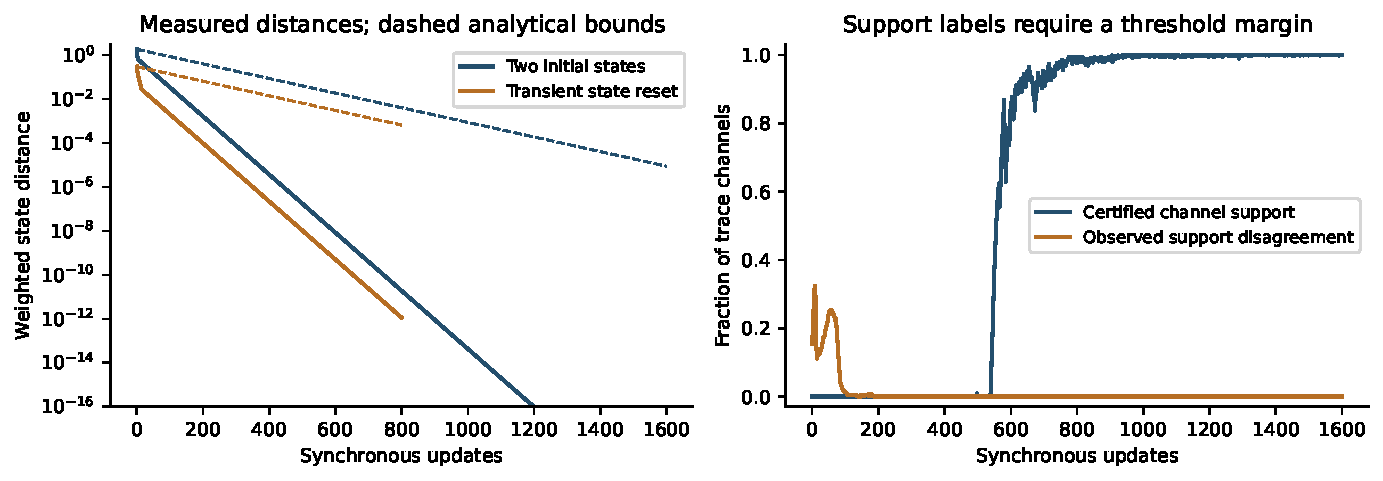
\includegraphics[width=\linewidth]{figures/guarantees.pdf}
\caption{Synchronization, transient reset recovery and support-margin certification. Dashed curves are derived upper bounds; solid curves are measured distances. Distances below $10^{-16}$ are plotted at that floor. A small state discrepancy does not automatically certify labels close to the threshold.}
\label{fig:guarantees}
\end{figure}

\subsection{Core ablations}
\begin{table}[!htbp]\centering\small
\caption{Core test NMSE: mean $\pm$ sample standard deviation across ten seeds. Lower is better. Values below $10^{-14}$ are displayed as such.}
\begin{tabular}{lccc}\toprule
Model & Delay & Lagged product & Covariance \\\midrule
Current input & $1.0010\pm0.0015$ & $1.0015\pm0.0024$ & $1.0167\pm0.0177$ \\
Linear delay bank & $<10^{-14}$ & $1.0111\pm0.0048$ & $1.0248\pm0.0270$ \\
Fixed activity & $0.7832\pm0.0168$ & $1.0045\pm0.0056$ & $0.3959\pm0.0531$ \\
Static budget control & $0.7905\pm0.0153$ & $1.0050\pm0.0056$ & $0.3842\pm0.0824$ \\
Trace observer & $0.7855\pm0.0179$ & $0.9462\pm0.0147$ & $0.0265\pm0.0086$ \\
Plastic activity & $0.7831\pm0.0169$ & $1.0042\pm0.0051$ & $0.3959\pm0.0531$ \\
Plastic joint & $0.7856\pm0.0179$ & $0.9462\pm0.0148$ & $0.0266\pm0.0087$ \\
\bottomrule\end{tabular}
\label{tab:core}
\end{table}
The trace observer reduces covariance NMSE from $0.3959$ for fixed activity to $0.0265$. This comparison combines access to 96 additional trace features with their distinct memory dynamics. It does not isolate a gain from network rewiring. The equal-feature comparison supplies that distinction: plastic joint and trace observer have nearly identical errors.

For covariance, the paired mean difference, plastic joint minus trace observer, is $+3.80\times10^{-5}$, with sample standard deviation $9.46\times10^{-5}$; plastic joint is better in only two of ten seeds. There is no consistent advantage for plastic feedback in this configuration. The delayed-sample task is solved by the linear delay bank, whereas the compact recurrent representations remain near NMSE $0.78$. The lagged-product error of trace models remains about $0.95$, a limited improvement over a constant predictor.

\begin{figure}[!htbp]\centering
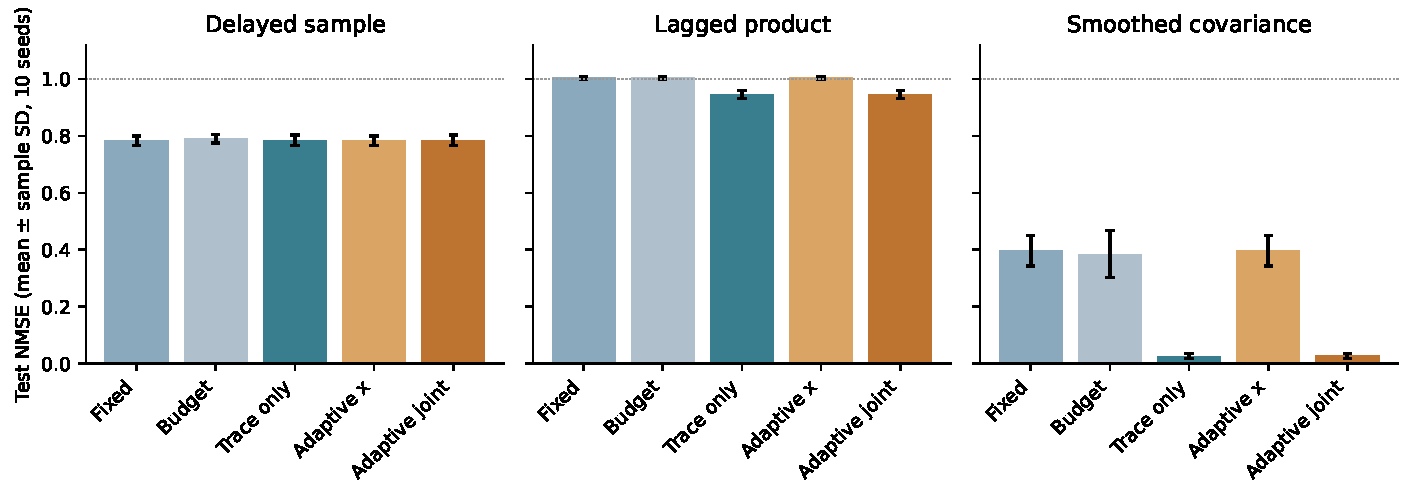
\includegraphics[width=\linewidth]{figures/ablations.pdf}
\caption{Mechanism ablations on the same ten input and graph seeds. Error bars show across-seed sample standard deviation, not confidence intervals. Trace access accounts for the prominent covariance improvement.}
\label{fig:ablations}
\end{figure}

\subsection{Hybrid evaluation and changing support}
\begin{table}[!htbp]\centering\small
\caption{Extension evaluation on ten new seeds. Task definitions are unchanged; models have different feature budgets.}
\begin{tabular}{lccc}\toprule
Model & Delay & Lagged product & Covariance \\\midrule
Plastic joint & $0.7917\pm0.0194$ & $0.9503\pm0.0134$ & $0.0264\pm0.0111$ \\
Trace observer & $0.7916\pm0.0194$ & $0.9503\pm0.0133$ & $0.0264\pm0.0111$ \\
Quadratic delay bank & $<10^{-14}$ & $<10^{-14}$ & $0.4534\pm0.0466$ \\
Hybrid memory & $<10^{-14}$ & $<10^{-14}$ & $0.0250\pm0.0076$ \\
\bottomrule\end{tabular}
\label{tab:extension}
\end{table}
The quadratic delay bank represents the first two targets exactly, and the fitted readout realizes them to numerical precision. Its finite history misses older contributions to exponential covariance, yielding mean NMSE $0.4534$. Adding observer traces produces the hybrid covariance error $0.0250$, while retaining the exact polynomial targets. The trace observer alone has covariance error $0.0264$ in this cohort. The central benefit is the coexistence of distinct memory capabilities, rather than a large extra covariance gain from combining them.

The active plastic support genuinely changes, but its activity is modest under the chosen independent inputs. In seed zero, the test mean fraction of active trace channels is approximately $0.0159$; the fraction of nonzero total weights is $0.3496$, compared with a backbone fraction of $1/3$. Many candidate channels remain below threshold. This explains why plastic feedback has little effect in these runs, without establishing that stronger plasticity would improve a different task.

\begin{figure}[!htbp]\centering
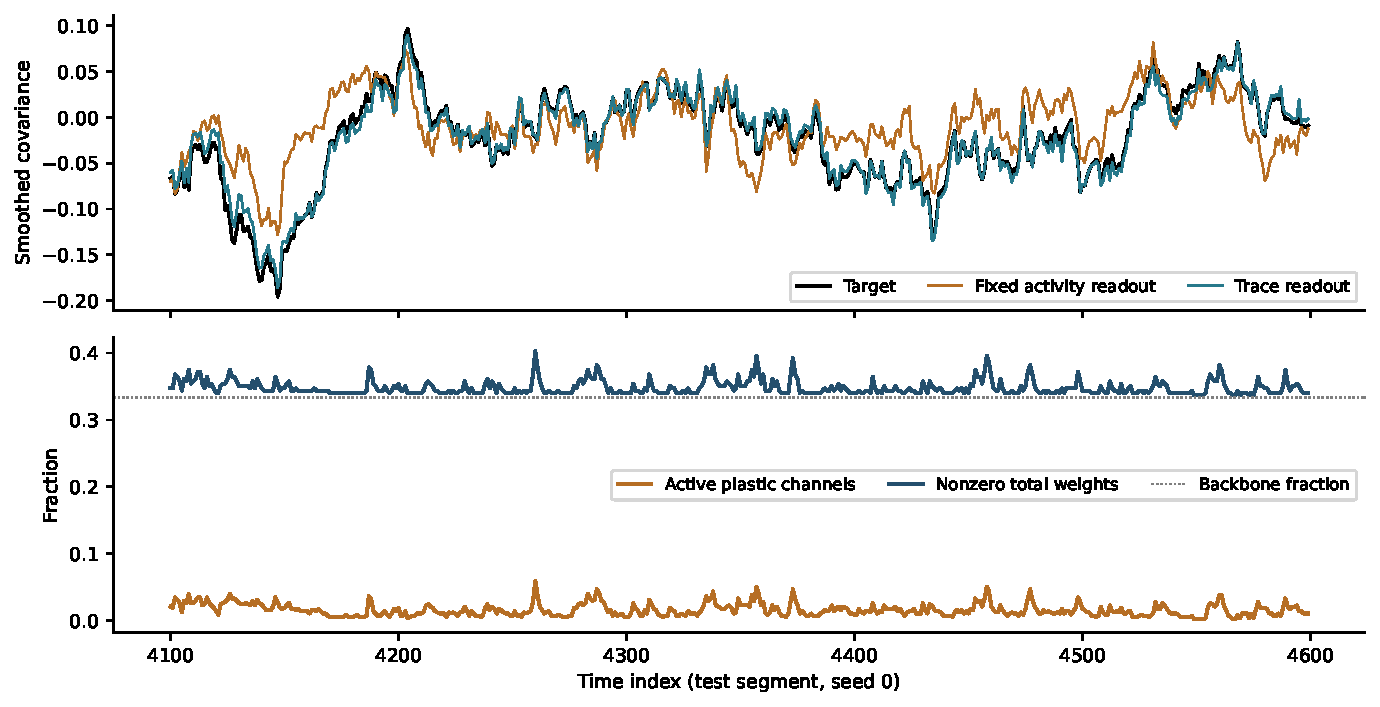
\includegraphics[width=\linewidth]{figures/behavior.pdf}
\caption{A saved test segment for seed zero. Top: covariance target and two readouts. Bottom: active channel fraction and nonzero total-weight fraction in the plastic model. These two support measures have different definitions.}
\label{fig:behavior}
\end{figure}
\FloatBarrier

\subsection{Clock semantics and exact-transition checks}
In 2000 random trials, the largest discrepancy in the subdivision identity \eqref{eq:refinement} was $4.45\times10^{-16}$; the affine implementation agreed within $1.12\times10^{-16}$. The largest excess over the contraction bound was $2.23\times10^{-16}$, consistent with roundoff and below the declared $3\times10^{-14}$ tolerance. No sampled invariant-box violation occurred. An independent adaptive DOP853 integration of the differential equations, with relative tolerance $10^{-12}$ and absolute tolerance $10^{-14}$, agreed with the closed transition within $6.37\times10^{-14}$ over 40 trials. Its comparison tolerance was $3\times10^{-11}$.

A 100-event composite stream was also processed with randomly subdivided held intervals. Preserving one graph/delay update per genuine event gave a maximum state discrepancy of $3.34\times10^{-16}$. Incorrectly treating every substep as an event created 465 events and a maximum discrepancy of $1.96$. This countercheck demonstrates why timestamp handling alone does not guarantee whole-architecture refinement invariance. Consistent relabeling of the graph, its parameters and state commuted with 100 updates exactly in the executed floating-point case. These tests verify the implemented contracts, not all possible schedules or hardware implementations.

\subsection{Multitemporal representation and head selection}
\begin{table}[!htbp]\centering\scriptsize
\caption{Irregular-duration test NMSE on fresh seeds 60--69, before the duration shift. Entries are mean $\pm$ sample standard deviation. Selected heads choose among the five preceding families using validation data only.}
\begin{tabular}{lrrrr}\toprule
Model & Event delay & Fast filter & Slow filter & Order \\\midrule
Event hybrid & $<10^{-14}$ & $0.395 \pm 0.033$ & $0.531 \pm 0.085$ & $0.7 \pm 0.03$ \\
Elapsed symmetric & $0.951 \pm 0.0074$ & $0.0024 \pm 9.8\times10^{-5}$ & $0.00464 \pm 0.00036$ & $1.02 \pm 0.021$ \\
Elapsed ordered & $0.952 \pm 0.0084$ & $0.0024 \pm 8.9\times10^{-5}$ & $0.0047 \pm 0.00035$ & $0.0157 \pm 0.0017$ \\
Elapsed quadratic & $0.958 \pm 0.0094$ & $0.00249 \pm 0.0001$ & $0.00537 \pm 0.00049$ & $0.131 \pm 0.013$ \\
Concatenated & $<10^{-14}$ & $0.00261 \pm 0.00048$ & $0.00774 \pm 0.0013$ & $0.0196 \pm 0.0015$ \\
Selected heads & $<10^{-14}$ & $0.0024 \pm 0.00011$ & $0.00502 \pm 0.0012$ & $0.0157 \pm 0.0017$ \\
\bottomrule\end{tabular}
\label{tab:multitime}
\end{table}
The event hybrid retains the six-event delay exactly but does not accurately resolve duration-dependent targets. Compact elapsed features accurately approximate both filters while failing to retrieve an exact event-index sample. The ordered representation achieves mean order-target NMSE $0.0157$, compared with $1.0213$ for its equal-dimension symmetric control. Quadratic combinations of means recover some order information, with error $0.1309$, but remain less accurate on this diagnostic. The two-interval example in Section~\ref{sec:clock} establishes a precise single-scale information distinction; the benchmark separately measures these finite feature banks.

\begin{table}[!htbp]\centering\scriptsize
\caption{The same trained models on independent streams with shorter event durations. There is no retraining, normalization change or reselection. NMSE is normalized by each shifted target's variance.}
\begin{tabular}{lrrrr}\toprule
Model & Event delay & Fast filter & Slow filter & Order \\\midrule
Event hybrid & $<10^{-14}$ & $2.2 \pm 0.22$ & $3.43 \pm 1.1$ & $13.1 \pm 3.2$ \\
Elapsed symmetric & $1.01 \pm 0.0091$ & $0.0107 \pm 0.0013$ & $0.0072 \pm 0.0021$ & $1.28 \pm 0.25$ \\
Elapsed ordered & $1.01 \pm 0.0085$ & $0.0107 \pm 0.0013$ & $0.0071 \pm 0.0022$ & $0.0278 \pm 0.0061$ \\
Elapsed quadratic & $1.01 \pm 0.0066$ & $0.0107 \pm 0.0013$ & $0.00718 \pm 0.0028$ & $0.283 \pm 0.038$ \\
Concatenated & $<10^{-14}$ & $0.0156 \pm 0.0013$ & $0.0361 \pm 0.011$ & $0.238 \pm 0.057$ \\
Selected heads & $<10^{-14}$ & $0.0116 \pm 0.0025$ & $0.0106 \pm 0.013$ & $0.0278 \pm 0.0061$ \\
\bottomrule\end{tabular}
\label{tab:shift}
\end{table}
Under shorter durations, the compact ordered representation reaches $0.0278$ order-target error, whereas concatenation rises to $0.2378$. This is an empirical limitation of the fitted concatenated representation under the specified shift, not a universal claim that additional features are harmful. The concatenated model is also substantially larger.

Validation selection chooses the event hybrid for exact delay and the ordered family for the order target in all ten routing seeds. It therefore retains both capabilities. Selection among filter heads varies: the slow target uses the symmetric family in five seeds, the ordered family in four and concatenation in one. That final choice incurs shifted slow-filter NMSE $0.0479$, despite being selected on the original validation regime. Consequently, selection does not guarantee shift-optimal behavior: its mean shifted slow-filter error is $0.0106$, compared with $0.00710$ for the fixed ordered family. No shifted labels enter the choice.

\begin{figure}[!htbp]\centering
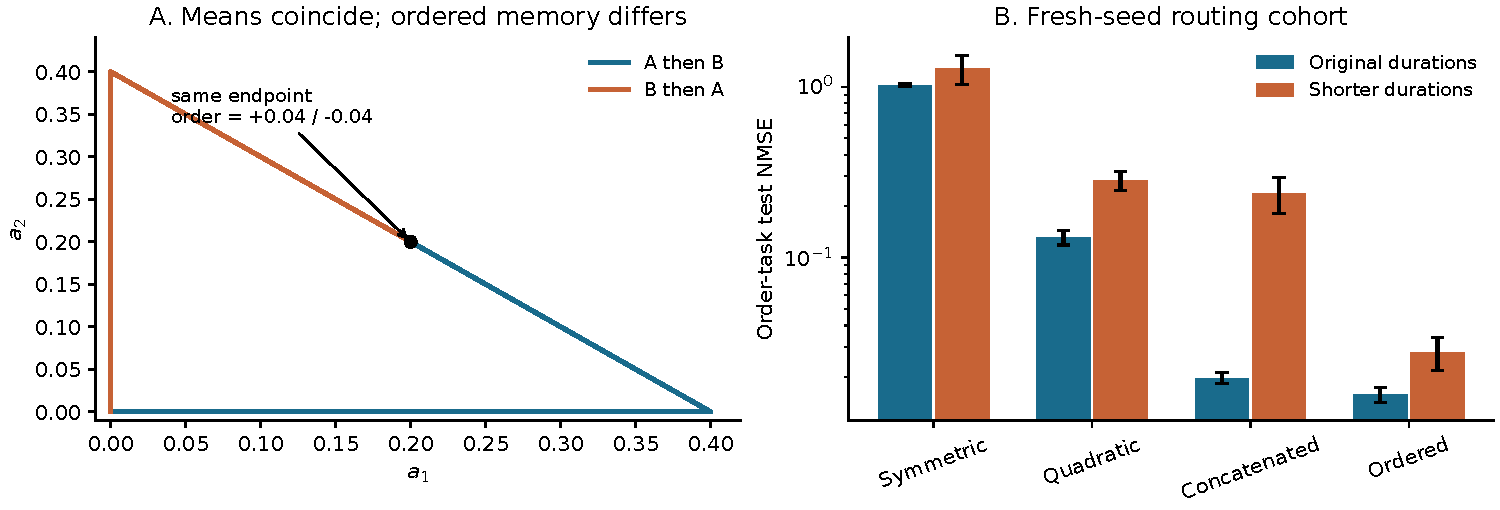
\includegraphics[width=\linewidth]{figures/multitime.pdf}
\caption{Order-sensitive memory. Left: two histories with identical final single-scale means and opposite ordered coordinates. Right: order-target errors across the ten routing seeds, with sample standard deviations, on the original and shorter-duration regimes. The task explicitly favors access to ordered fading information.}
\label{fig:multitime}
\end{figure}
\FloatBarrier

\subsection{Conditional output ranges and selective retrieval}
The algebraic checks use 100 randomized six-event boxes with six uncertain scalars each and 3000 additional interior completions. No completion left its vertex range at tolerance $10^{-12}$. Restriction by \eqref{eq:restrictvertices} agreed with explicit replay within $1.78\times10^{-15}$, and subdivision while retaining the same uncertain input identities agreed within $4.45\times10^{-16}$. All 64 vertices of a separate rational reference with three events and decay $1/2$ agreed exactly with fraction arithmetic. Empty evidence ranges and conflicting duplicate readings were rejected; identical duplicate queries left the result unchanged.

\begin{table}[!htbp]\centering\small
\caption{Partial-observation study: resolved signs out of 128 cases after four or eight exact archive queries. ``Box at 8'' uses ordinary interval propagation on the same acquired inputs. Relative width is the mean ratio to each case's initial vertex width.}
\begin{tabular}{llrrrr}\toprule
Observable & Query rule & At 4 & At 8 & Box at 8 & Width at 8 \\\midrule
Order state & Random & 17 & 48 & 32 & 0.2881 \\
Order state & Recent first & 57 & 108 & 85 & 0.0560 \\
Order state & Minimax width & 68 & 111 & 86 & 0.0430 \\
Frozen readout & Random & 11 & 44 & 5 & 0.2713 \\
Frozen readout & Recent first & 19 & 65 & 11 & 0.1650 \\
Frozen readout & Minimax width & 33 & 92 & 22 & 0.0869 \\
\bottomrule\end{tabular}
\label{tab:partial}
\end{table}
At eight queries, the minimax policy resolves the frozen readout in 92 cases, versus 65 for recent-first and 44 for random retrieval. For the single-scale ordered state the corresponding counts are 111, 108 and 48: recency is already a strong control for this fading observable. The minimax improvement is therefore task dependent. Its relative remaining width is $0.0869$ for the frozen head, compared with $0.1650$ and $0.2713$. The ordinary interval enclosure resolves only 22 frozen-head cases under the same minimax acquisitions, illustrating the cost of discarding dependencies.

Midpoint filling gives the wrong sign in 37 of 128 ordered-state cases and 32 of 128 frozen-readout cases. The range-based procedure reports no incorrect resolved signs among the 9984 evaluated case/task/policy/budget states. These are repeated evaluations of 128 cases, not 9984 independent samples. Soundness is conditional on the declared input box and model; the theorem, rather than an empirical zero-error rate, supplies the exact-arithmetic implication. With all twelve missing entries acquired, all methods resolve all cases, as expected from complete information.

\begin{figure}[!htbp]\centering
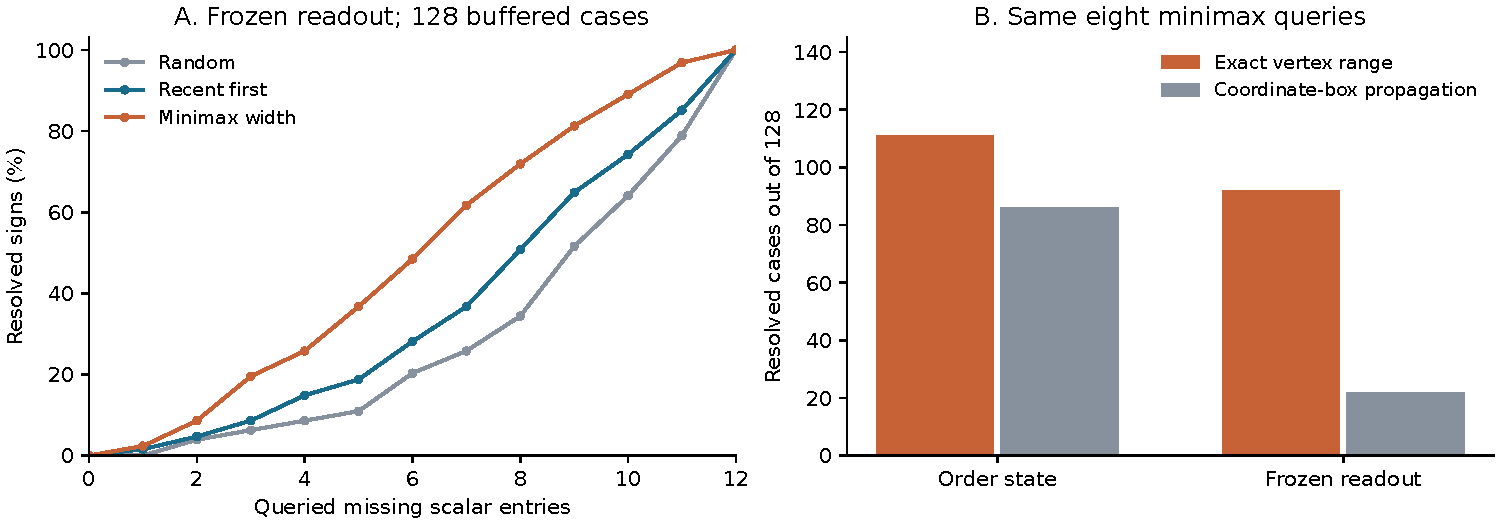
\includegraphics[width=\linewidth]{figures/partial_observation.pdf}
\caption{Selective retrieval from an immutable input buffer. Left: resolved signs of the frozen elapsed-time readout as more missing scalar entries are acquired. Right: exact vertex ranges versus ordinary interval propagation after eight queries, for the same minimax-selected entries. The reference sign belongs to the complete-input model output.}
\label{fig:partial}
\end{figure}
The numerical reference uses float64, an explicit decision margin and comparison tolerances; it does not implement outward-rounded interval arithmetic. Thus its executed checks are numerical evidence for the real-arithmetic result, not machine-verified bounds on all rounding and transcendental-function errors. This experiment uses 4096 initial vertex completions per audited function. Section~\ref{sec:scalable} supplies the different enclosure strategy evaluated below for larger missing sets.
\FloatBarrier

\subsection{External classification and the role of the observer}
\begin{table}[!htbp]\centering\small
\caption{Original external test splits. Entries give correct records and accuracy; balanced accuracy is also shown for the unequal RacketSports classes.}
\begin{tabular}{lrrr}\toprule
Model & RacketSports & Bal. acc. & BasicMotions \\
\midrule
Flattened ridge & 116/152 (76.32\%) & 77.51\% & 31/40 (77.5\%) \\
Mean memory & 110/152 (72.37\%) & 74.04\% & 30/40 (75.0\%) \\
Ordered memory & 121/152 (79.61\%) & 80.90\% & 23/40 (57.5\%) \\
Fixed trace observer & 130/152 (85.53\%) & 86.44\% & 38/40 (95.0\%) \\
Euclidean 1-NN & 126/152 (82.89\%) & 83.72\% & 24/40 (60.0\%) \\
\bottomrule\end{tabular}
\label{tab:externalclass}
\end{table}
The fixed trace observer performs best among these five evaluated controls on both datasets: 130/152 correct RacketSports records and 38/40 BasicMotions records. Ordered memory exceeds the mean-only head on RacketSports (121 versus 110), but falls below it on BasicMotions (23 versus 30). The latter failure occurs despite higher training-fold accuracy for the ordered family, so validation success alone does not establish transfer to the fixed test split. The selected ridge penalties are reported in the saved classification table; no test-driven correction is applied.

These results support continued investigation of readable recurrent traces, while limiting the claim for compact ordered features. The comparison uses one fixed observer graph and two small datasets, with no participant-disjoint resampling or matched compute budget. The supplied records contain no exact train/test duplicates; that check does not establish participant independence. No superiority over modern trained time-series classifiers follows. The polynomial acquisition result concerns the ordered head; the nonlinear observer is assessed separately using Section~\ref{sec:observeraudit}.

\subsection{Scalable bounds: computational gain and conservative decisions}
The quadratic compiler was checked in 2000 direct transition/polynomial comparisons with two to four channels and four events. For 100 boxes with eight unknown scalars, all 256 vertices per box remained inside the coefficient enclosure. Maximum polynomial/transition discrepancy was $2.67\times10^{-15}$, and recentering discrepancy was $1.78\times10^{-15}$. The maximum numerical excess in nested-range checks was $1.78\times10^{-15}$; the two-channel implementation agreed with the existing interface exactly in the executed comparisons. These tests use tolerance $10^{-10}$ and complement the algebraic derivation.

\begin{table}[!htbp]\centering\small
\caption{Mean numbers of missing scalar values retrieved before the ordered classifier's winner is resolved. Lower is better. Every entry averages all original test records for the specified mask.}
\begin{tabular}{llrrrr}\toprule
Dataset & Mask & Missing & Random & Recent & Coefficient \\
\midrule
RacketSports & Random half & 90 & 87.61 & 84.78 & 83.27 \\
RacketSports & Middle half & 90 & 87.47 & 85.74 & 83.65 \\
BasicMotions & Random half & 300 & 296.00 & 295.55 & 283.88 \\
BasicMotions & Middle half & 300 & 295.70 & 294.57 & 284.10 \\
\bottomrule\end{tabular}
\label{tab:externalacq}
\end{table}
The coefficient policy uses fewer queries on average than both controls in all four dataset/mask combinations. Nevertheless, it still retrieves approximately 92.5--94.7\% of the missing values. No case is resolved at three quarters of the query budget under any policy. Thus the representation removes the exponential enumeration cost, but the conservative box and coefficient enclosure provide little early stopping in these tests. A smaller certified set of plausible completions or a tighter enclosure could improve this, but neither is assumed here.

Across all paths, the saved ranges contain the corresponding complete-input score differences at tolerance $10^{-9}$, and no resolved class contradicts its complete-input model winner. There are 155232 evaluated audit states and 154080 queried values across 192 test records, two masks and three policies. They are repeated evaluations, not independent statistical trials. Correctness against external labels remains exactly the separate issue in Table~\ref{tab:externalclass}; at full acquisition, every case is resolved, including cases the classifier labels incorrectly.

\begin{figure}[!htbp]\centering
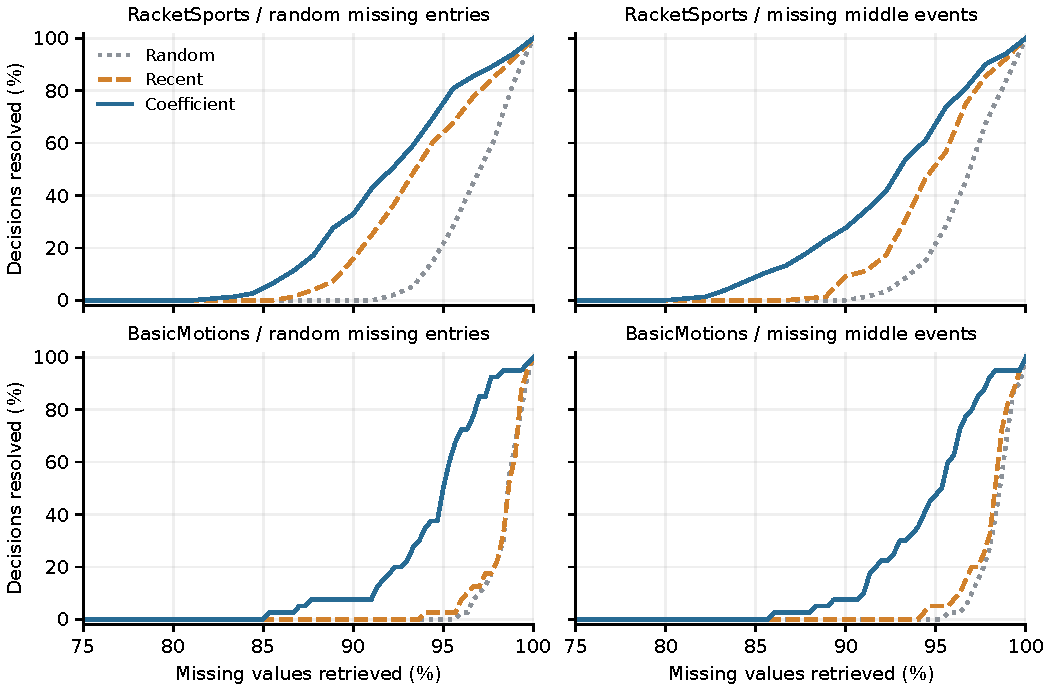
\includegraphics[width=\linewidth]{figures/external_acquisition.pdf}
\caption{Fraction of model decisions resolved versus fraction of missing scalar values retrieved. The horizontal axis shows the last quarter of the acquisition budget; all earlier states are unresolved. The coefficient policy uses the maximum enclosing width over class pairs as a surrogate; it does not directly optimize the stopping cost.}
\label{fig:externalacq}
\end{figure}

The executed synthetic cost check, with seven repeats per size, computes one scalar enclosure and all candidate query scores. Median time increases from 0.0435 ms at $J=12$ to 5.55 ms at $J=768$; the corresponding stored coefficient arrays use 1256 bytes and 4.72 MB (decimal). These are local reference timings, excluding compilation, data loading and the classifier. The six-output external acquisition runs take approximately 34.7 s and 233.1 s respectively on the execution environment, without a hardware-portability claim. The cost check demonstrates usable sizes beyond the enumerator's $J\leq16$ guard; it does not make the scalar enclosure exact.

Verification reloads all delivered external ranges, answers and decisions, checks nesting and recomputes the class verdicts. Final training fits and classifier outputs are replayed; full policy/bound reconstruction covers the first and last test record of each dataset, with every mask and policy. Cross-validation is not rerun in this output-replay stage. The separate algebraic tests compare direct transitions with polynomial evaluation and vertex references.

\subsection{Nonlinear observer: valid bounds, limited early resolution}
The independent small observer checks cover 1488 complete inputs, including all 768 box vertices and 720 random interior inputs. No score difference or forward-reference derivative lies outside its interval at tolerance $10^{-10}$. Direct score evaluation agrees with the original recurrence; singleton range and derivative discrepancies are at most $8.89\times10^{-16}$. Sixty exact-query restrictions satisfy nesting and the frozen derivative width bound. Additional controls exercise endpoint rates $\alpha=1$, $\beta=1$ and exact cancellation between equally weighted trace dynamics with opposite head coefficients. In the cancellation control, the compiled and hybrid widths are zero while the basic enclosure has maximum width 3.826. These checks complement Proposition~\ref{prop:observerbox}; they are not exhaustive floating-point verification.

\begin{table}[!htbp]\centering\small
\caption{Frozen nonlinear observer: mean scalar queries until its winner is resolved using hybrid bounds. All 152 or 40 original test cases enter each mean. The classifier is not refitted.}
\begin{tabular}{llrrrr}\toprule
Dataset & Mask & Missing & Random & Recent & Derivative \\ \midrule
RacketSports & Random half & 90 & 89.95 & 89.95 & 89.45 \\
RacketSports & Middle half & 90 & 89.99 & 89.96 & 89.93 \\
BasicMotions & Random half & 300 & 298.60 & 295.60 & 295.40 \\
BasicMotions & Middle half & 300 & 298.77 & 297.88 & 297.30 \\
\bottomrule\end{tabular}\label{tab:observeracq}
\end{table}
The derivative rule has the smallest mean stopping count among these three policies in all four comparisons, but the savings are small. It retrieves 98.47--99.92\% of the missing inputs on average. No policy resolves any case by three quarters of its budget. Relative to random acquisition, the mean savings are only 0.50 and 0.07 scalars for the two RacketSports masks, and 3.20 and 1.48 for BasicMotions. A different head and different enclosure are involved in Table~\ref{tab:externalacq}; its query counts are not a like-for-like verifier comparison.

\begin{table}[!htbp]\centering\small
\caption{Bound ablation on identical derivative-selected query paths. Entries are mean stopping counts. Structured bounds combine the original trace intervals with the compiled history enclosure; hybrid bounds additionally intersect the centered derivative enclosure.}
\begin{tabular}{llrrr}\toprule
Dataset & Mask & Basic & Structured & Hybrid \\ \midrule
RacketSports & Random half & 89.99 & 89.99 & 89.45 \\
RacketSports & Middle half & 90.00 & 90.00 & 89.93 \\
BasicMotions & Random half & 296.90 & 296.90 & 295.40 \\
BasicMotions & Middle half & 298.52 & 298.52 & 297.30 \\
\bottomrule\end{tabular}\label{tab:observerablation}
\end{table}
Trace-history combination alone does not change the stopping counts in these tests, although it is algebraically useful for the reverse recurrence. The derivative intersection yields a modest improvement. These results do not support a claim that the implemented bounds are tight enough for efficient partial-record classification. They also do not prove that no stronger verifier or narrower justified completion set could decide earlier.

\begin{table}[!htbp]\centering\small
\caption{Observer decisions resolved by hybrid bounds under synthetic coordinatewise uncertainty around the complete normalized record. Entries are resolved cases / total cases, not correct external labels.}
\begin{tabular}{lrrrrrr}\toprule
Dataset / radius & 0 & 0.005 & 0.01 & 0.02 & 0.05 & 0.10 \\ \midrule
RacketSports & 152/152 & 66/152 & 0/152 & 0/152 & 0/152 & 0/152 \\
BasicMotions & 40/40 & 15/40 & 5/40 & 0/40 & 0/40 & 0/40 \\
\bottomrule\end{tabular}\label{tab:observernoise}
\end{table}
At radius 0.005 the method resolves 66/152 RacketSports cases and 15/40 BasicMotions cases; at 0.01 it resolves zero and five. Failure to resolve is inconclusive: it is neither an observed label error nor evidence that an admissible perturbation changes the model's winner. These intervals are imposed computationally and do not estimate a physical sensor's error distribution.

The observer study evaluates 155232 input-box states, each with three enclosures, hence 465696 range sets, and retrieves 154080 scalar values. Every saved range contains its complete-input score differences at tolerance $10^{-9}$; no resolved verdict contradicts that model. The complete-input observer scores are unchanged. The original classification errors therefore remain possible even for resolved cases. The study runs in approximately 90.1 s and 271.8 s on the reference environment; these local timings include all policies and budgets, not only early-stopped deployment.

Output verification reloads every range, verdict and answer, checks nesting and query membership, and recomputes verdicts. It reconstructs complete paths for the first and last record of each dataset under all masks and policies. The derivative policy is recomputed, and all evidence records are replayed. Additional interior completions test large-box inclusion on those paths. These numerical box computations have no directed-rounding guarantee. The affine comparison and the separate validated point checks follow below; POPQORN and branch-and-bound implementations are not benchmarked.

\subsection{Affine bounds and actual ambiguity}
The scalar relaxation checks cover 1000 intervals and 101000 sampled points, including singleton intervals. Twelve small graphs supply 1488 complete-input checks. Singleton bounds and independent forward-reference gradients agree to $8.89\times10^{-16}$, at test tolerance $10^{-10}$. These checks support the implementation of Proposition~\ref{prop:affinehistory}, without changing its real-arithmetic status.

\begin{table}[!htbp]\centering\small
\caption{Mean missing scalars retrieved for the unchanged full-record observer. The affine column intersects the new bound with the hybrid enclosure and previous valid bounds. Budgets are 90 for RacketSports and 300 for BasicMotions.}
\begin{tabular}{llrrrr}\toprule
 & & \multicolumn{2}{c}{Derivative policy} & \multicolumn{2}{c}{Decision policy} \\
Dataset & Mask & Hybrid & Affine & Hybrid & Affine \\\midrule
RacketSports & Random half & 89.45 & 88.97 & 89.45 & 88.95 \\
RacketSports & Middle half & 89.93 & 89.51 & 89.93 & 89.46 \\
BasicMotions & Random half & 295.40 & 292.20 & 295.32 & 292.12 \\
BasicMotions & Middle half & 297.30 & 295.23 & 297.30 & 295.23 \\
\bottomrule\end{tabular}
\label{tab:relaxed}
\end{table}
Affine relaxation improves stopping under either policy, but the decision-focused policy adds little (Table~\ref{tab:relaxed}). Together they require 97.375--99.401\% of missing values on average. No case resolves by $\lfloor3J/4\rfloor$. All 103488 input-box states, 206976 enclosure sets and 102720 answers were reloaded and checked. Complete first/last-record replay covers 3120 queries; the largest range discrepancy is $3.42\times10^{-13}$. Every resolved class agrees with the unchanged complete-input head within the numerical checking protocol.

\begin{table}[!htbp]\centering\small
\caption{Input boxes with two Arb-validated compatible completions having different strict winners, along the decision-focused query path. Denominators are 152 RacketSports or 40 BasicMotions records per row. Columns specify already acquired missing values, with initial budget $J=90$ or $300$.}
\begin{tabular}{llrrrrr}\toprule
Dataset & Mask & $0$ & $\lfloor J/2\rfloor$ & $\lfloor3J/4\rfloor$ & $\lfloor9J/10\rfloor$ & $J-6$ \\\midrule
RacketSports & Random half & 152 & 152 & 152 & 150 & 143 \\
RacketSports & Middle half & 152 & 152 & 152 & 144 & 107 \\
BasicMotions & Random half & 40 & 40 & 35 & 15 & 1 \\
BasicMotions & Middle half & 40 & 40 & 39 & 12 & 1 \\
\bottomrule\end{tabular}
\label{tab:witness}
\end{table}
The witness search validates ambiguity in 1719 of 1920 examined boxes (Table~\ref{tab:witness}). These are repeated information states, not independent observations. Both initial masks and their halfway-query states are ambiguous for every tested record. Near three quarters of the budget, all RacketSports states and 35/40 or 39/40 BasicMotions states remain demonstrably ambiguous. Their non-resolution cannot be eliminated by a tighter sound verifier on the same box. The remaining 201 searches establish no conclusion about ambiguity.

These witnesses concern independent unknown coordinates in $[-1,1]$. They do not establish that the competing completions are physically plausible movement trajectories. A justified temporal or sensor constraint could shrink that set, but was not imposed here. Nor do these findings prove optimality of the query paths. Their concrete implication is that improving interval tightness alone does not address all of the observed delay.

\subsection{A blockwise prediction--retrieval tradeoff}
\begin{table}[!htbp]\centering\small
\caption{Different complete-record classifiers on the same external splits and missing masks. Retrieval columns give mean missing scalars read, out of 90 or 300. Full-record affine uses the decision-focused policy. Block models use strict integer vote dominance with validated local winners. Each audit preserves its own classifier.}
\begin{tabular}{llrrr}\toprule
Dataset & Classifier & Correct & Random half & Middle half \\\midrule
RacketSports & Full record, affine & 130/152 & 88.95 & 89.46 \\
RacketSports & Block mean & 68/152 & 78.97 & 68.61 \\
RacketSports & Block observer & 113/152 & 72.95 & 65.84 \\
BasicMotions & Full record, affine & 38/40 & 292.12 & 295.23 \\
BasicMotions & Block mean & 29/40 & 213.45 & 147.00 \\
BasicMotions & Block observer & 38/40 & 199.40 & 136.50 \\
\bottomrule\end{tabular}
\label{tab:blockresults}
\end{table}
On BasicMotions, the block observer correctly classifies 38/40 records and agrees with the original observer on all 40 predictions. It retrieves 199.4/300 missing values under the random mask and 136.5/300 under the middle mask, or 66.47\% and 45.50\%. Relative to the original hybrid/derivative audit, the additional-value count falls by 32.50\% and 54.09\%, respectively. Early stopping occurs in 37/40 and 34/40 records. This is equality of observed predictions on this split, not equivalence of the classifiers as functions or a population non-inferiority result.

On RacketSports, retrieval falls to 72.95/90 and 65.84/90, or 81.06\% and 73.16\%, but correct classifications decline from 130 to 113. The new model corrects ten formerly wrong cases and loses 27 formerly correct ones. Thus five local resets are not a uniformly beneficial replacement for the full-record observer. This comparison does not separate the effects of reset boundaries, block-label training and vote quantization.

The mean-only block control obtains 68/152 and 29/40 correct records, below the block observer's 113/152 and 38/40. It also requires more queries under both masks. This supports the value of the richer local representation within this specific control comparison, with 150 versus six non-intercept features; it does not isolate traces from activities or establish equal-compute superiority.

All 960 observer block winners and all 960 mean-control block winners were validated using 100-bit Arb arithmetic. Integer stopping was checked exhaustively for all $4^5$ vote assignments and all $2^5$ initial known-block subsets: 32768 cases, including multiclass ties. An independent edge-by-edge Arb recurrence at 160-bit precision supplies 60 score references contained in the 100-bit point enclosures. The block preservation proof is independent of these finite tests. Rounding control applies to the evaluated local votes and resulting discrete stopping decisions, not to every earlier continuous enclosure in this manuscript.

\subsection{Retaining context through prefix votes}\label{sec:prefixresults}
\begin{table}[!htbp]\centering\small
\caption{Previously examined tasks: all declared classifier families. BA is balanced accuracy. Random and Middle give the mean percentage of initially missing scalars retrieved; Stream gives the mean percentage of the full record observed from its start. Tie-aware stopping preserves each family's own complete prediction. The full observer is a full-read cost baseline.}
\begin{tabular}{llrrrrr}\toprule
Dataset & Classifier & Correct & BA (\%) & Random & Middle & Stream \\\midrule
RacketSports & Full observer & 130/152 & 86.44 & 100.00 & 100.00 & 100.00 \\
 & Reset blocks & 113/152 & 75.04 & 79.96 & 70.88 & 79.47 \\
 & Shared prefix & 128/152 & 85.56 & 73.08 & 85.79 & 72.63 \\
 & Stage prefix & 131/152 & 87.35 & 70.86 & 84.39 & 70.26 \\
 & Stage mean & 97/152 & 64.90 & 79.49 & 91.05 & 79.21 \\
\midrule
BasicMotions & Full observer & 38/40 & 95.00 & 100.00 & 100.00 & 100.00 \\
 & Reset blocks & 38/40 & 95.00 & 66.47 & 44.75 & 66.50 \\
 & Shared prefix & 39/40 & 97.50 & 66.64 & 78.25 & 67.00 \\
 & Stage prefix & 40/40 & 100.00 & 66.85 & 77.50 & 67.00 \\
 & Stage mean & 32/40 & 80.00 & 67.98 & 79.00 & 68.00 \\
\bottomrule\end{tabular}
\label{tab:prefixdevelopment}
\end{table}
Continuous-state prefix voters recover much of the predictive information lost by reset blocks on RacketSports (Table~\ref{tab:prefixdevelopment}). The primary stage-specific model obtains 131/152 correct decisions and retrieves 63.78/90 missing scalars under the random mask and 75.95/90 under the middle mask. These are 70.86\% and 84.39\%, with early decisions on 137/152 and 89/152 records. Relative to the full observer's 130 correct decisions, this is a net gain of one on the observed split, not a population improvement: ten formerly correct records become wrong and eleven formerly wrong records become correct. The shared-head variant obtains 128 correct, showing that preserving state with a matched head budget already recovers much, but not all, of the reset model's deficit.

On BasicMotions, the stage-specific prefix model obtains 40/40 correct decisions, correcting both full-observer errors and losing none. Retrieval is 200.55/300 and 232.50/300 scalars, or 66.85\% and 77.50\%, with 36/40 and 30/40 records stopped early. The shared-head version obtains 39/40. The sample is small and previously examined; a perfect test count is not a bound on future error. Reset blocks remain less expensive under the middle mask, retrieving 44.75\% with tie-aware stopping while correctly classifying 38/40. The prefix model therefore trades additional central-window retrieval for better observed accuracy.

\begin{table}[!htbp]\centering\small
\caption{First project evaluation on two additional public tasks under the same fixed protocol. Columns and guarantees are as in Table~\ref{tab:prefixdevelopment}. Results include the primary candidate's NATOPS accuracy loss.}
\begin{tabular}{llrrrrr}\toprule
Dataset & Classifier & Correct & BA (\%) & Random & Middle & Stream \\\midrule
NATOPS & Full observer & 155/180 & 86.11 & 100.00 & 100.00 & 100.00 \\
 & Reset blocks & 137/180 & 76.11 & 82.91 & 79.67 & 82.91 \\
 & Shared prefix & 159/180 & 88.33 & 78.83 & 93.93 & 78.86 \\
 & Stage prefix & 150/180 & 83.33 & 79.05 & 94.09 & 79.08 \\
 & Stage mean & 144/180 & 80.00 & 82.29 & 96.27 & 82.29 \\
\midrule
Epilepsy & Full observer & 121/138 & 87.74 & 100.00 & 100.00 & 100.00 \\
 & Reset blocks & 133/138 & 96.44 & 63.62 & 38.69 & 63.78 \\
 & Shared prefix & 133/138 & 96.50 & 62.30 & 73.17 & 62.46 \\
 & Stage prefix & 129/138 & 93.62 & 62.78 & 73.61 & 62.90 \\
 & Stage mean & 60/138 & 45.27 & 64.29 & 74.92 & 64.36 \\
\bottomrule\end{tabular}
\label{tab:prefixnew}
\end{table}
The new tasks do not identify a universal winner (Table~\ref{tab:prefixnew}). On NATOPS, the shared prefix head reaches 159/180 correct against 155/180 for the full observer, retrieving 78.83\% of randomly missing inputs and 93.93\% of centrally missing inputs. The predeclared primary stage-specific head obtains 150/180, five fewer than the full observer despite identical mean cross-validation accuracy to the shared prefix head. This negative outcome is retained. On Epilepsy, both reset blocks and shared prefix heads obtain 133/138 against 121/138 for the full observer; stage-specific heads obtain 129/138. Shared-prefix retrieval is 62.31\% under random missingness and 73.17\% under the central mask. Reset blocks are much cheaper on that central mask, at 38.69\%. Thus maintaining context can improve prediction, but forces earlier gaps to be filled before later prefix evidence becomes usable.

\begin{table}[!htbp]\centering\small
\caption{Paired prediction changes relative to the full observer. Lost counts formerly correct cases made wrong; Gained counts formerly wrong cases made correct. Changed also includes changes between two incorrect labels. Net is the change in the number correct.}
\begin{tabular}{llrrrr}\toprule
Dataset & Prefix head & Changed & Lost & Gained & Net \\\midrule
RacketSports & Shared & 28 & 15 & 13 & -2 \\
RacketSports & Stage & 21 & 10 & 11 & +1 \\
BasicMotions & Shared & 1 & 0 & 1 & +1 \\
BasicMotions & Stage & 2 & 0 & 2 & +2 \\
NATOPS & Shared & 20 & 8 & 12 & +4 \\
NATOPS & Stage & 20 & 12 & 7 & -5 \\
Epilepsy & Shared & 13 & 0 & 12 & +12 \\
Epilepsy & Stage & 15 & 3 & 11 & +8 \\
\bottomrule\end{tabular}
\label{tab:prefixpaired}
\end{table}
Table~\ref{tab:prefixpaired} separates aggregate accuracy from prediction identity. For example, the shared prefix head loses no formerly correct Epilepsy case and corrects twelve errors, but changes thirteen labels because one wrong label changes to another. Equal or improved aggregate counts do not imply pointwise preservation of the original head. Only the new ensemble's own full prediction is preserved by its stopping rule.

The stage-specific cumulative-mean control is less accurate than both prefix observers on every tested split: 97/152, 32/40, 144/180 and 60/138 correct. This supports the usefulness of the recurrent representation within the declared comparison. The feature counts differ, and activity, traces, nonlinear input responses and effective memory scales are not individually isolated here. It does not establish superiority over competitive trained sequence classifiers.

\begin{figure}[!htbp]\centering
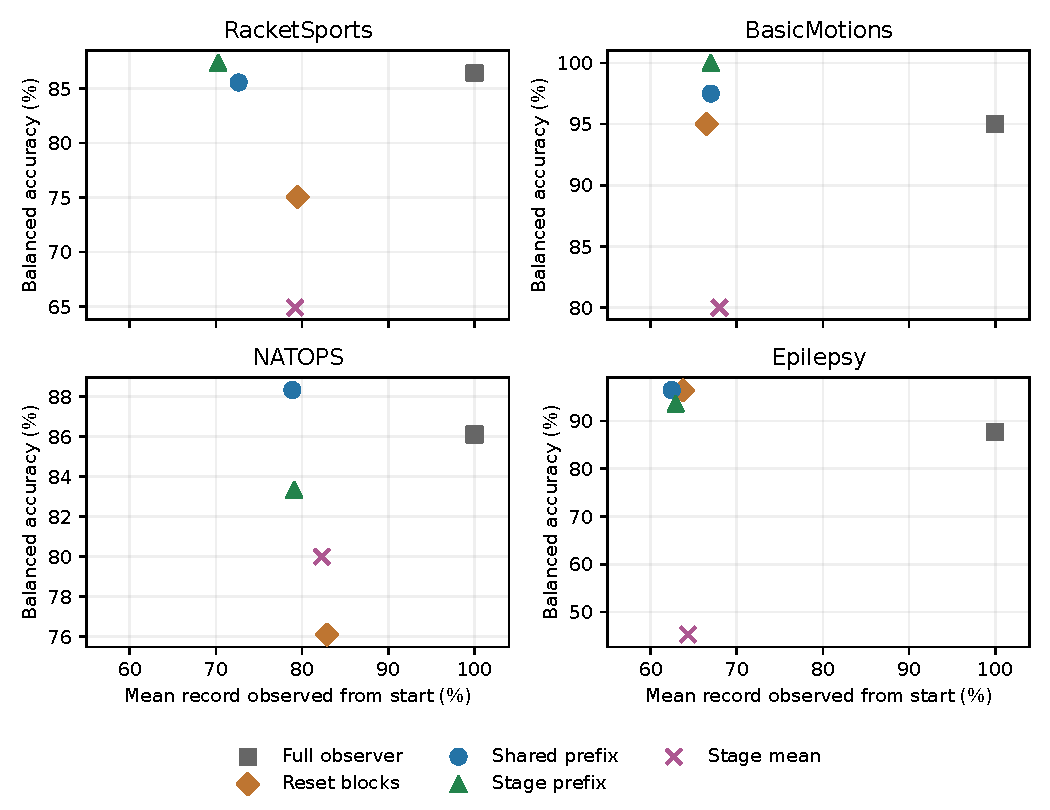
\includegraphics[width=0.95\linewidth]{figures/prefix_tradeoff.pdf}
\caption{Accuracy and acquisition when no inputs are initially known. Every point represents a complete fixed classifier and its exact vote-based stopping policy, except the full observer, which reads the full record. Movement left reduces the mean fraction observed; movement up increases balanced accuracy. The patterns are task dependent. No test-selected envelope or routing policy is fitted.}
\label{fig:prefixtradeoff}
\end{figure}
Starting with no observed input, stage-specific prefixes read mean record fractions of 70.26\%, 67.00\%, 79.08\% and 62.90\% in dataset order (Figure~\ref{fig:prefixtradeoff}). The complete labels are unchanged. This condition distinguishes actual prefix exposure from savings obtained when later measurements were already available. It still assumes a known record horizon, exact observations and the frozen training transform.

The tie-aware rule reduces queries in 180 of the 6120 paired record/mask/ensemble comparisons and never increases them. This is a deterministic refinement of the same fixed voters; it changes neither fitted models nor complete predictions. Its logical sharpness is limited to the abstraction of unrestricted unread votes, as stated in Proposition~\ref{prop:tievote}.

\subsection{Validation of continuous-prefix decisions}
All 10710 point winners across the five families and four datasets were validated at 100-bit precision without a fallback. Exact dyadic comparisons of the stored outward endpoints confirm their strict winners. Independent replay reproduced every final fit and complete score array, with zero discrepancy in this environment, and all 15300 stopping records were checked for unique queries, mask membership, input-dependency closure and agreement with the complete classifier. The final-fit replay does not rerun cross-validation training; it recomputes the selection from the saved fold scores. All fold fits were executed in the original benchmark.

Finite enumeration checks the tie-aware rule against every completion of all 19932 partial five-vote states for four and six classes, totaling 281600 completions. Four future-input perturbations check prefix causality on an independent 11-event example. Twenty score references from separate complete-prefix Arb runs are contained in the one-pass checkpoint enclosures. Finally, the first and last test record of each task supply 168 point-winner replays at 160-bit precision; their score intervals lie inside the saved 100-bit intervals. These executed tests complement the counting proof. They do not validate all continuous-box routines or establish physical uncertainty coverage.

\subsection{Delayed local execution}
All four delayed-message runs satisfy both the history-envelope bound and its $B+L$-step reduction at tolerance $10^{-12}$. Final paired distances lie between $3.47\times10^{-4}$ and $3.72\times10^{-4}$; the theoretical final bounds range from 0.640 to 1.057. The bound is therefore conservative rather than an estimate of typical synchronization speed.

With constant input $(0.2,-0.3)$, 30000 round-robin delayed updates at $L=48$ approach a 6000-step synchronous fixed-point reference to weighted error $4.59\times10^{-10}$. A deliberately starved cell retains activity discrepancy one. Under changing input, otherwise identical executions with ages zero and 48 differ by as much as 0.231 in weighted state distance. These controls distinguish stability under a shared execution contract from equality of computations under different timing semantics.
\FloatBarrier

\subsection{Conditional decisions across two model domains}\label{sec:domainresults}
\begin{table}[htbp]\centering\small
\caption{Exhaustive finite-model query costs: mean/worst. T is conservative transport; E is event order; D is the domain predicate and G the frozen Gabriel readout. $K$ is the number of independent metadata values. Every policy stops on target agreement; constant queries are skipped.}\label{tab:domain}
\begin{tabular}{lrrrrrr}\toprule
Task & $K$ & Fixed & Reverse & Entropy & EC$^2$ & Minimax \\ \midrule
T--D & 1 & 2.83/3 & 1.00/1 & 1.00/1 & 1.00/1 & 1.00/1 \\
T--D & 4 & 2.83/3 & 2.00/2 & 1.00/1 & 1.00/1 & 1.00/1 \\
T--D & 16 & 2.83/3 & 2.00/2 & 2.00/2 & 1.00/1 & 1.00/1 \\
\addlinespace
T--G & 1 & 1.67/3 & 1.72/3 & 1.22/2 & 1.22/2 & 1.50/2 \\
T--G & 4 & 1.67/3 & 2.72/4 & 1.44/3 & 1.22/2 & 1.50/2 \\
T--G & 16 & 1.67/3 & 2.72/4 & 2.22/3 & 1.22/2 & 1.50/2 \\
\addlinespace
E--D & 1 & 1.50/2 & 3.00/3 & 1.50/2 & 1.50/2 & 1.50/2 \\
E--D & 4 & 1.50/2 & 4.00/4 & 2.00/3 & 1.50/2 & 1.50/2 \\
E--D & 16 & 1.50/2 & 4.00/4 & 2.50/3 & 2.50/3 & 1.50/2 \\
\addlinespace
E--G & 1 & 1.92/3 & 2.67/3 & 1.92/3 & 1.25/2 & 1.25/2 \\
E--G & 4 & 1.92/3 & 3.67/4 & 2.67/4 & 1.25/2 & 1.25/2 \\
E--G & 16 & 1.92/3 & 3.67/4 & 2.92/4 & 2.25/3 & 1.25/2 \\
\bottomrule\end{tabular}
\end{table}

Every one of the 17640 primary acquisition paths ends in a correct conditional target decision. This is exhaustive agreement with the specified finite target tables, not a measured population accuracy. The optimal worst-cost policy uses one query for the transport predicate and at most two for each of the other three domain/target combinations. Its mean costs are respectively $1$, $3/2$, $3/2$ and $5/4$ for transport/domain, transport/Gabriel, event/domain and event/Gabriel, independent of the number of nuisance values.

Table~\ref{tab:domain} also records contrary evidence to universal policy superiority. At $K=1$, entropy and EC$^2$ both have transport/Gabriel mean cost $11/9$, below the minimax policy's $3/2$, while all three have worst cost two. The minimax tie rule does not optimize averages. The chronological fixed policy already attains the minimax mean for the event-order predicate. Reverse order can be especially costly because it queries the appended metadata first.

With $K=16$, entropy queries the irrelevant tag in every case. EC$^2$ does so for both event targets, although it avoids that query on transport. A large metadata partition removes many weighted cross-target pairs without changing the set of possible targets; this is compatible with its different greedy objective. For the event predicate, minimax decides after 1.5 queries on average and entropy and EC$^2$ after 2.5. Every minimax event-predicate decision still leaves multiple physical event histories. Thus target agreement is useful before full-history identification, even after unobservable aliases are excluded from that comparison.

\begin{table}[htbp]\centering\small
\caption{Exploratory removal of independent queries, $K=16$. Counts before/after refer to distinct labelled rows and memoized Bellman states. Mean costs after reduction are shown for the two greedy policies; minimax costs are unchanged.}\label{tab:domainreduction}
\begin{tabular}{lrrrr}\toprule
Task & Labelled rows & Bellman states & Entropy & EC$^2$ \\ \midrule
T--D & 288/18 & 799/47 & 1.00 & 1.00 \\
T--G & 288/18 & 782/46 & 1.22 & 1.22 \\
E--D & 384/24 & 1887/111 & 1.50 & 1.50 \\
E--G & 384/24 & 1853/109 & 1.92 & 1.25 \\
\bottomrule\end{tabular}
\end{table}

The exploratory product test removes the metadata coordinate in every catalogue and the constant initial empty-cell query in transport. At $K=16$, the labelled observation tables shrink from 288 to 18 rows for transport and from 384 to 24 rows for event order. Memoized Bellman states fall from 799 to 47 and 782 to 46 for the two transport targets, and from 1887 to 111 and 1853 to 109 for the event targets. These are exact state-count reductions, not measured sensor or hardware speedups.

For the event predicate, reduction brings the entropy and EC$^2$ means to 1.5 queries. For the corresponding Gabriel target, the EC$^2$ mean falls from 2.25 to 1.25. The optimal worst-cost values remain unchanged in all twelve catalogues. For that Gabriel target, entropy still costs $23/12$ queries on average, versus $5/4$ for EC$^2$ and minimax. Removing nuisance variables therefore does not solve every greedy-choice limitation. Figure~\ref{fig:domain} shows the four matched comparisons.

\begin{figure}[htbp]\centering
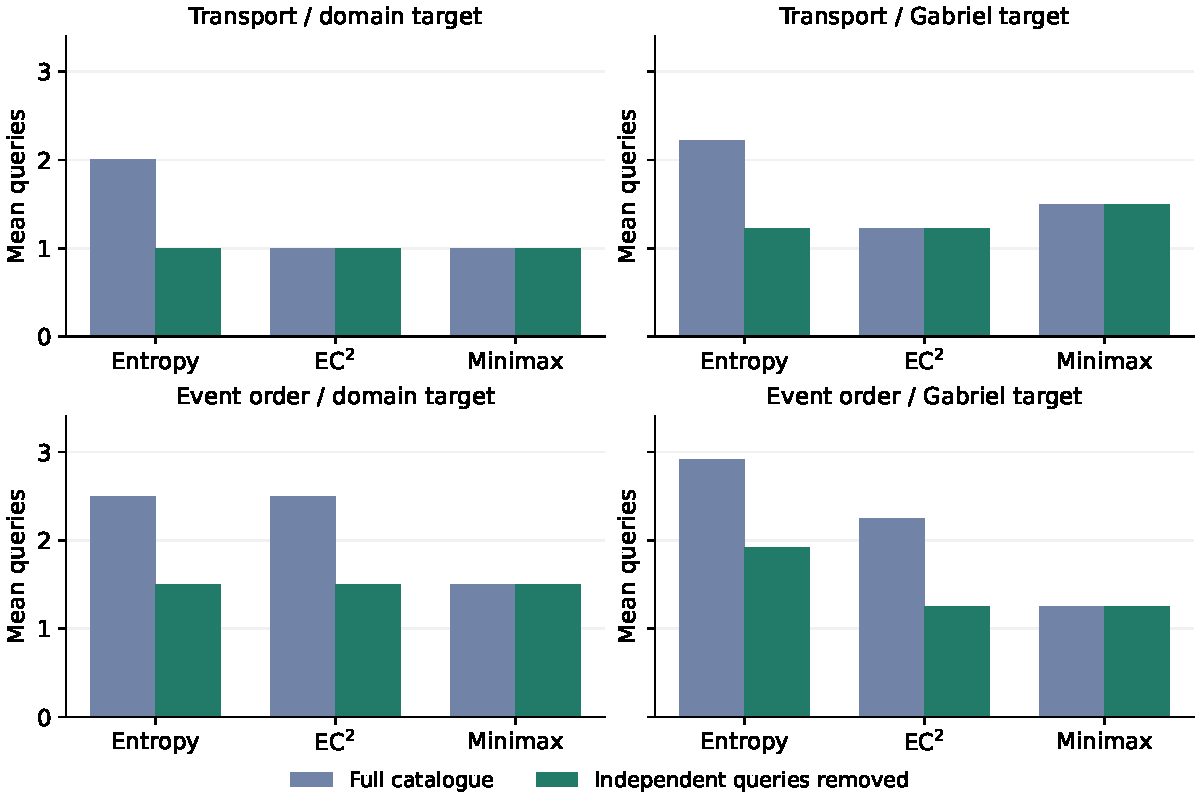
\includegraphics[width=0.94\linewidth]{figures/domain_observation.pdf}
\caption{Mean query costs before and after the exploratory independent-query reduction, with 16 metadata values. Every bar averages all raw catalogue cases, and every decision is checked against its frozen target. This controlled nuisance experiment is not a benchmark of real-world domain transfer.}\label{fig:domain}
\end{figure}

\subsection{Checks of the finite observation interface}
An independent bounded-depth decision-tree existence oracle checks the exact planner on all $2^{12}\binom42=24576$ tables with four hypotheses, three binary queries and balanced binary targets. Every optimal cost, including impossibility, agrees. The reduced tables are also checked against this same oracle. Exact rational checks verify conservation, bounds and the dissipation identity for all 144 transport pair updates. A persistent one-bit-error example has eight expanded hypotheses; three tests determine its binary target in the worst case.

All 17640 primary paths and 17640 reduced paths are replayed using direct filtering of original row sets, independently of saved bit masks. Query choices are recomputed, costs summed, realised-history retention checked and target agreement verified. The 42 Gabriel point evaluations are recomputed at both precisions. Another 1008 policy paths compare raw and quotient tables, preserving choices and weighted costs for minimax, EC$^2$ and entropy.

The negative checks retain mixed-target histories with identical past observations, reject premature or conflicting evidence, and distinguish event time from receipt time. They demonstrate both detectable model conflict and an undetectable out-of-model target discrepancy. XOR-dependent tests and inexpensive correlated metadata fail the product-removal criterion as required. A full-support but nonfactorized weighted example confirms that support factorization is not automatically prior independence. These are implemented checks of explicitly stated cases; they do not validate an unrestricted causal or physical model.

\subsection{Damped phase memory and the coordinate budget}\label{sec:phaseresults}
\begin{table}[!htbp]
\centering\small
\begin{tabular}{lrrrrrr}
\toprule
Dataset & $n$ & Trace & Real & Phase & Real+trace & Phase+trace \\
\midrule
RacketSports & 152 & 130 & 113 & 115 & 130 & 125 \\
BasicMotions & 40 & 38 & 29 & 30 & 36 & 36 \\
NATOPS & 180 & 155 & 164 & 160 & 166 & 164 \\
Epilepsy & 138 & 121 & 65 & 71 & 118 & 124 \\
\bottomrule
\end{tabular}
\caption{Correct test decisions. Standalone banks have 16 real state coordinates per input channel; the two hybrid heads add the same number of features to the unchanged trace observer. All families are reported, without test-based selection.}
\label{tab:phase_main}
\end{table}

Adding a real temporal bank to the trace observer changes NATOPS from 155 to 166 correct cases, with 14 gains and 3 losses. The phase hybrid reaches 164, with 4 gains and 6 losses relative to the real hybrid. Thus this improvement does not require a rotating kernel. On Epilepsy, the phase hybrid reaches 124 versus 118 for the real hybrid and 121 for the trace reference, but remains below the earlier continuous-prefix results. On RacketSports it loses five net cases against the real hybrid; BasicMotions is tied at 36, below the trace reference's 38. These comparisons support optional, task-tested representations rather than a replacement of the existing default by a uniformly superior family.

\begin{table}[!htbp]
\centering\small
\begin{tabular}{lrrrrrr}
\toprule
Dataset & Real 3 & Phase 3 & Real 5 & Phase 5 & Real 7 & Phase 7 \\
\midrule
RacketSports & 113 & 112 & 110 & 115 & 115 & 116 \\
BasicMotions & 30 & 30 & 32 & 30 & 31 & 23 \\
NATOPS & 165 & 146 & 165 & 160 & 165 & 156 \\
Epilepsy & 69 & 72 & 73 & 63 & 66 & 72 \\
\bottomrule
\end{tabular}
\caption{State-budget ablation: correct test decisions of standalone banks. Budgets count real memory coordinates per input channel, not the dimension of the full Gabriel system. Five is neither uniformly best nor a demonstrated universal optimum.}
\label{tab:phase_budget}
\end{table}

The five-coordinate phase bank is useful as a concrete compact realization, but is not uniformly best even in the declared nested family. The seven-coordinate phase bank is best among its three small variants on RacketSports; the three- and five-coordinate variants tie on BasicMotions; five is best on NATOPS; three and seven tie on Epilepsy. Different pole choices or tasks could change these rankings. No universal dimension optimum follows from this finite comparison or from the dimension bound in \eqref{eq:dimensionbound}.

\begin{figure}[!htbp]
\centering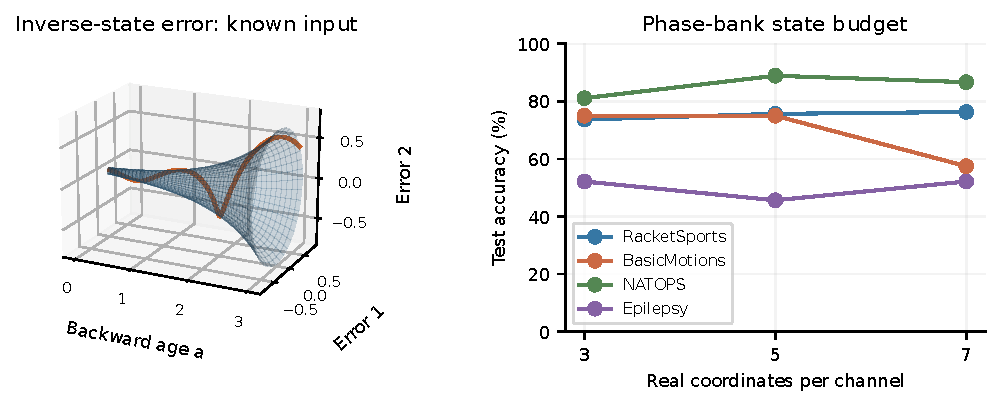
\includegraphics[width=\linewidth]{figures/phase_geometry.pdf}
\caption{Left: illustrative inverse-state error geometry, $R(a)=0.04e^a$, with a rotating error vector of angular frequency $4$. The widening reflects conditioning under known intervening input; it is not an empirical image or recovered history. Right: executed standalone phase-bank comparisons on the original test splits. Coordinate counts are per input channel.}
\label{fig:phasegeometry}
\end{figure}

\subsection{Validated continuous-box decisions for linear banks}
\begin{table}[!htbp]
\centering\small
\begin{tabular}{lrrrr}
\toprule
Dataset & Real random & Real middle & Phase random & Phase middle \\
\midrule
RacketSports & 88.33 & 85.21 & 86.56 & 84.93 \\
BasicMotions & 90.64 & 90.49 & 90.03 & 90.71 \\
NATOPS & 84.39 & 84.06 & 86.77 & 86.27 \\
Epilepsy & 65.14 & 62.94 & 82.93 & 81.60 \\
\bottomrule
\end{tabular}
\caption{Mean percentage of missing scalars retrieved by the coefficient policy for the standalone 16-coordinate banks. Every stop is validated over its continuous input box. These heads have their own predictive accuracy (Table~\ref{tab:phase_main}); their counts cannot be substituted for the nonlinear observer or hybrid.}
\label{tab:phase_retrieval}
\end{table}

Coefficient-guided retrieval uses 62.94--90.71\% of the missing scalars across the two banks, masks and tasks. Reverse temporal order uses 79.60--98.07\%. All 4080 reported stops preserve their own complete linear-bank decisions over the declared continuous boxes. Their prediction quality is given separately in Table~\ref{tab:phase_main}; in particular the standalone Epilepsy heads are much less accurate than the trace-based alternatives. Reduced retrieval for a different weak predictor is not an improvement of the full observer's accuracy--acquisition tradeoff.

Arb establishes 5610 strict point winners, covering all eleven families on 510 test records, and all 4080 strict box certificates at 100 bits. No precision escalation is needed; the smallest certified stopping margin exceeds $4.98\times10^{-6}$. Independent real-matrix-exponential replay differs from the stored features by at most $1.73\times10^{-15}$. All 44 final ridge heads are refitted from saved training features and all acquisition paths replayed with independent query-order reconstruction. The 1760 fold fits belong to the primary experiment; a second complete cross-validation run is not claimed.

The mechanism checks cover 300 randomized continuous transitions, all eight bank variants, 20 complete eight-variable vertex boxes and 40 paired event/subdivision transitions. The largest absolute discrepancy against the real augmented matrix exponential is below $3.57\times10^{-14}$. Separate counterexamples demonstrate expansion under unrestricted positive-gradient feedback and under an unsuitable Euler step, phase aliasing modulo $2\pi$, and lost uncertainty cancellation after incorrectly splitting a shared variable. Analytical bounds establish the universal statements; these numerical cases verify their implementation within the stated tolerances.

\subsection{Operational cycles and orientation-consistent memory}\label{sec:orientationresults}
Exact binary elimination gives boundary ranks $(12,18)$ for the full disk and $(11,12)$ for the operational annulus, confirming \eqref{eq:annulusdisk}. Both underlying graphs have diameter three and vertex/edge connectivity four. Removing the reference changes radius two to three and replaces the unique reference center by all twelve operational vertices. The full graph's supplied spectra are reproduced to their displayed rounding precision. The distinction concerns executable incidence, not a presumed privilege of a prime number of addresses.

All 4096 face-flat operational assignments pass every triangle check, but exactly 2048 have negative global holonomy. A check that equates local triangle consistency with positive global orientation would therefore accept an incorrect global claim on half this explicitly enumerated set. The additional ring bit separates the two cases exactly. The positive representative's double cover has two connected 12-vertex components, each of diameter three; the negative representative's cover is connected with 24 vertices and diameter six. Independent all-pairs distances verify every returned route and every unreachable verdict.

All 32 neural trajectories agree under the coordinate transformation, frame change and double-cover construction at the declared $10^{-12}$ tolerance. The paired implementations give zero binary64 discrepancy in these runs; independent dense extended-precision replay of all 8192 stored states has maximum absolute error $6.89\times10^{-16}$. Every paired initialization obeys its analytical contraction envelope. The transported pooled diagnostic is unchanged by frame conventions, while the untransported control changes in these same runs. These checks establish implementation consistency with Proposition~\ref{prop:frame}; they do not measure a classification gain or supply a machine-verified real-arithmetic dynamics proof.

\subsection{Minimum-cost observation of a global orientation bit}
\begin{table}[!htbp]\centering
\caption{Exact cycle-parity observation. Each entry is queries / total cost and applies to all 4096 compatible sign assignments. The random control is one fixed permutation, not an average over policies.}
\begin{tabular}{lrrrr}\toprule
Access model & Optimal & Lexical & Reverse & Random \\\midrule
Unit costs & 6 / 6 & 14 / 14 & 6 / 6 & 11 / 11 \\
Inner edges cost 9 & 6 / 6 & 14 / 62 & 6 / 6 & 11 / 43 \\
Inner edges unavailable & 6 / 6 & 12 / 12 & 6 / 6 & 14 / 14 \\
\bottomrule\end{tabular}\label{tab:orientationqueries}
\end{table}

Six edge queries suffice in all three access profiles, and their minimum cost is six. For unit costs, the lexical order reads fourteen values and the fixed random order eleven. Reverse order reads the outer ring first and already attains the optimum. Increasing inner-edge cost raises the lexical and random totals to 62 and 43, while both the optimizer and reverse order retain cost six. Unavailable inner edges leave the target observable through other representatives; withholding all three reports across one seam instead makes it unobservable. No policy is assigned a definite target in that case.

The independent replay verifies all 49152 target decisions and exact row-combination certificates. Every proper prefix of every saved stopping set remains compatible with both target values. All 42504 five-query subsets are insufficient, agreeing with the seam-set lower bound. The additional finite oracle checks 80 affine systems and 960 evidence states, including explicit opposite-parity completions, conflicting evidence and unavailable targets. Equal repeated observations are idempotent; contradictory duplicates produce an exact conflict certificate.

\begin{figure}[!htbp]
\centering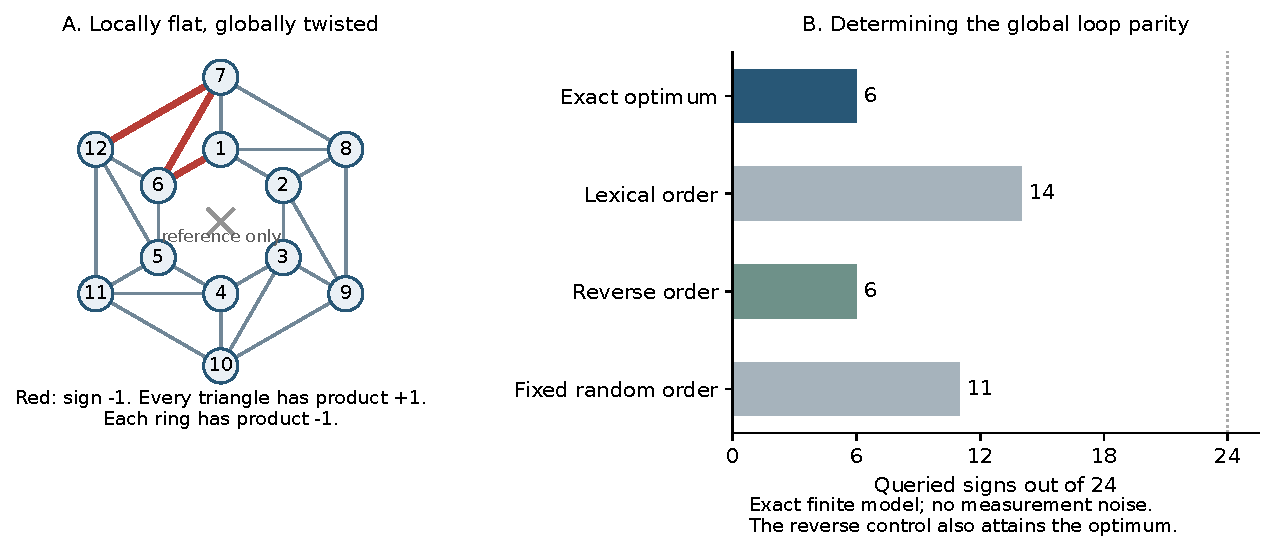
\includegraphics[width=\linewidth]{figures/orientation_transport.pdf}
\caption{Specified orientation model and exhaustive query study. The annulus permits flat triangle transports with a negative global loop. Under unit costs, six observed signs determine that loop parity while eighteen remain unread; a suitable fixed order also attains this optimum. These are exact conditional model results, not movement-classification measurements.}\label{fig:orientation}
\end{figure}

The supplied one-edge defect illustrates the remaining coverage boundary. A hidden inner-ring sign is reversed while observed outer-ring signs remain unchanged. The declared flat model still determines a parity, but the defect violates that model and reverses the actual inner-loop target. Section~\ref{sec:robustorientation} instead identifies a latent target under explicitly modeled report errors; it does not identify that target with the loop parity of an altered physical configuration. The six-query result complements the earlier acquisition studies and does not replace their observed retrieval percentages.

\subsection{Robust decisions and adaptive query savings}\label{sec:robustresults}
\begin{table}[!htbp]\centering
\caption{Exact one-error orientation decisions on 102400 latent-record/error cases per policy. All policies have zero wrong or unresolved outputs within the declared model. Means use the uniform finite catalogue, not an estimated deployment error distribution.}
\label{tab:robustorientation}
\begin{tabular}{lrrr}\toprule
Policy & Clean report & Maximum & Catalogue mean \\\midrule
Two rings + minimax & 12 & 17 & 14.24 \\
Two rings + EC$^2$ & 12 & 17 & 14.24 \\
Two rings + lexical & 12 & 24 & 15.56 \\
Lexical robust scan & 18 & 24 & 20.72 \\
Complete robust read & 24 & 24 & 24.00 \\
\bottomrule\end{tabular}
\end{table}

The minimax and EC$^2$ continuations both return the correct latent target on all 102400 cases. They stop at twelve reports in 53248 cases, sixteen in 16384 and seventeen in 32768. Every clean report stops at twelve, attaining the clean-record lower bound. The worst-case saving against a fixed sufficient set is seven of 24 reports, or $29.17\%$; the catalogue mean of 14.24 reports is a finite weighting convention, not a measured operational average. Neither exact minimax planning nor this experiment establishes an advantage over EC$^2$, which attains the same complete distribution.

The lexical continuation reaches 24 in its worst case. A lexical scan of all edge coordinates with robust stopping averages 20.72 and also reaches 24. These controls separate the contribution of ring structure from the subsequent query rule. The complete-read baseline always uses 24. All five policies remain correct within their common declared one-error model. These are acquisition counts, not measurements of total computation time.

The independent checks validate 512000 saved paths, 701 explicit binary certificates and all 289 Bellman states. The generic affine oracle resolves 1489 cases, preserves ambiguity in 2044 and finds 1267 conflicts, matching complete feasible-record filtering in all 4800 cases. It rejects 9045 altered certificates and ten invalid API requests. These checks substantiate the implementation; the universal distance and clean-record bounds are established analytically above.

\begin{figure}[!htbp]
 \centering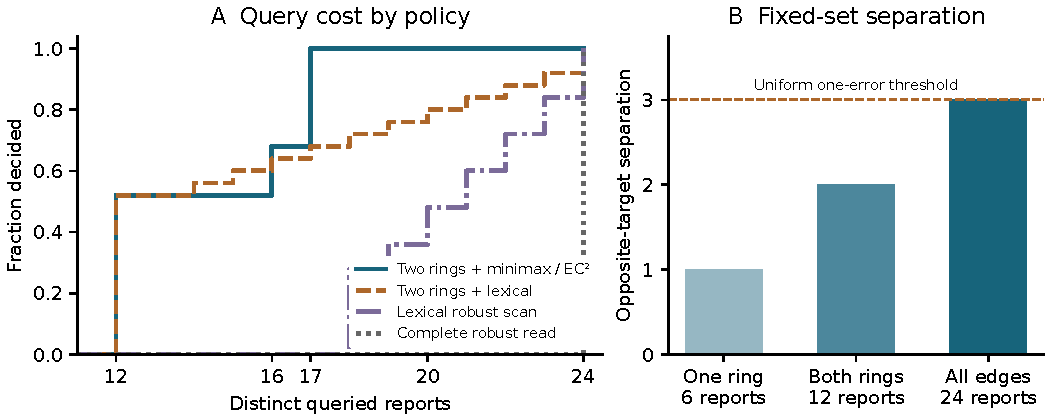
\includegraphics[width=\linewidth]{figures/robust_orientation.pdf}
 \caption{Bounded-error orientation observation. Left: exact cumulative query counts in the declared finite catalogue. The minimax and EC$^2$ curves coincide. Right: projected opposite-target separations for three fixed sets. Uniform correction of one error requires separation at least three, although particular reports can be decided earlier.}
 \label{fig:robustorientation}
\end{figure}

The budget stress test produces 70 wrong outputs from the one-error two-ring policy among the 276 two-error patterns, and 36 wrong outputs from the one-error full-read decoder. These are explicit failures outside the declared budget, not failures of the bounded-error implication. With budget two and complete reports, the exact observer returns 240 correct targets and retains 36 ambiguities; it issues no wrong known verdict. The remaining ambiguities have compatible opposite-target witnesses and cannot be resolved solely by reading the same reports again. Thus improved acquisition has a precise error contract and an explicit boundary beyond which certainty is unwarranted.

\FloatBarrier
\subsection{Exact risk calculations and conditional financial decisions}\label{sec:portfolioresults}
The optimizer supplies 768 exact risk certificates for 128 records, three actions and two horizons, with 176 distinct loss vectors. In this portfolio table, every convex-hull risk equals the largest individual-model CVaR: the strict mixture gap is zero in all 768 entries. Thus the general counterexample in \eqref{eq:mixturecounterexample} corrects an invalid shortcut but supplies no additional risk increment in this particular financial cohort.

\begin{table}[!htbp]\centering\small
\caption{Exhaustive acquisition costs. Finance uses 128 records at $\epsilon=2$, $K=25$; inspection uses 16 records. Means use uniform catalogue weights. The strict-label policies ($\dagger$) impose the stronger identification requirement described in Section~\ref{sec:decisionregions}. All policies satisfy the specified conditional action contract.}\label{tab:portfoliocosts}
\begin{tabular}{@{}lrrrr@{}}
\toprule
& \multicolumn{2}{c}{Portfolio ($n=128$)} & \multicolumn{2}{c}{Inspection ($n=16$)} \\
\cmidrule(lr){2-3}\cmidrule(lr){4-5}
Policy & Mean & Worst & Mean & Worst \\
\midrule
Minimax & $8$ & $9$ & $5/2$ & $3$ \\
Fixed & $69/8$ & $12$ & $17/4$ & $6$ \\
Reverse & $23/4$ & $9$ & $7/2$ & $5$ \\
Hypothesis entropy & $69/8$ & $12$ & $4$ & $4$ \\
Strict minimax$^{\dagger}$ & $8$ & $9$ & $7/2$ & $5$ \\
Strict EC$^2$$^{\dagger}$ & $153/16$ & $12$ & $9/2$ & $6$ \\
Full book & $10$ & $10$ & $5$ & $5$ \\
\bottomrule
\end{tabular}

\end{table}
The primary financial model admits a certified action in 96 records and no listed feasible action in 32. Every policy reaches the correct status and, where available, a member of the record's acceptable set. Regional minimax has worst cost nine and mean cost eight, against the minimum static full-book recovery cost ten. The full-book set reads cash, existing protection, liquidity and the joint position registry. A reversed query order also has worst cost nine and has a lower mean, $23/4$. Thus exact worst-cost optimality does not establish superior average acquisition, and the computationally simpler reversed order matches the worst-cost bound in this cohort. Canonical query-index tie-breaking in the minimax routine does not minimize a secondary average-cost objective.

Fixed order and hypothesis entropy have worst cost twelve and mean $69/8$; both retrieve the irrelevant tag on all 128 records. Strict-label minimax has the same worst and mean costs as regional minimax. Its stronger stopping objective therefore costs no more under that policy in the primary financial setting. Strict-label EC$^2$ has mean $153/16$ and worst cost twelve. These comparisons do not evaluate HEC or DiRECt, and the strict-label controls do not solve the same stopping problem as the regional policies.

Returned actions need not coincide across policies. For example, primary minimax selects retain in eight cases and reduce by half in 88, whereas reversed order selects reduce by half in all 96 feasible cases. Both satisfy the same completion-wise tolerance and absolute limit. This is preservation of acceptability, not preservation of a unique full-information action or evidence that the selected portfolio will realize a particular return.

\begin{table}[!htbp]\centering\small
\caption{Financial tolerance and absolute-limit controls. Counts exhaust the same 128 records. Increasing tolerance leaves the optimal worst acquisition cost unchanged here; lowering the absolute limit increases the number of blocked records.}\label{tab:portfoliocontrols}
\begin{tabular}{@{}rrrrrrrr@{}}
\toprule
& & & & \multicolumn{2}{c}{Minimax} & \multicolumn{2}{c}{Reverse} \\
\cmidrule(lr){5-6}\cmidrule(lr){7-8}
$\varepsilon$ & $K$ & Known & Blocked & Mean & Worst & Mean & Worst \\
\midrule
$2$ & $25$ & $96$ & $32$ & $8$ & $9$ & $23/4$ & $9$ \\
$0$ & $25$ & $96$ & $32$ & $8$ & $9$ & $25/4$ & $9$ \\
$6$ & $25$ & $96$ & $32$ & $8$ & $9$ & $23/4$ & $9$ \\
$2$ & $15$ & $24$ & $104$ & $55/8$ & $9$ & $43/8$ & $9$ \\
\bottomrule
\end{tabular}

\end{table}
For $K=25$, changing $\epsilon$ from zero to two or six leaves optimal worst cost at nine; the implemented minimax policy retains mean eight. The monotonicity in Proposition~\ref{prop:regionpreserve} permits equality; overlapping acceptable regions do not guarantee useful savings in every domain. At $K=15$, only 24 records admit an action and 104 are blocked. Regional minimax still has worst cost nine, with mean $55/8$, while reversed order averages $43/8$. Faster decisions can therefore reflect early identification of an infeasible action menu, not a better economic outcome.

In the industrial adapter, regional minimax uses worst cost three and mean $5/2$, compared with worst cost five for both strict-label minimax and complete physical-record recovery. All 16 records admit an acceptable action. This supplies a concrete case where accepting a common near-optimal action reduces the observation requirement. It demonstrates contract reuse and the effect of overlapping action regions in a second constructed model, not learned transfer to industrial operations.

\begin{figure}[!htbp]\centering
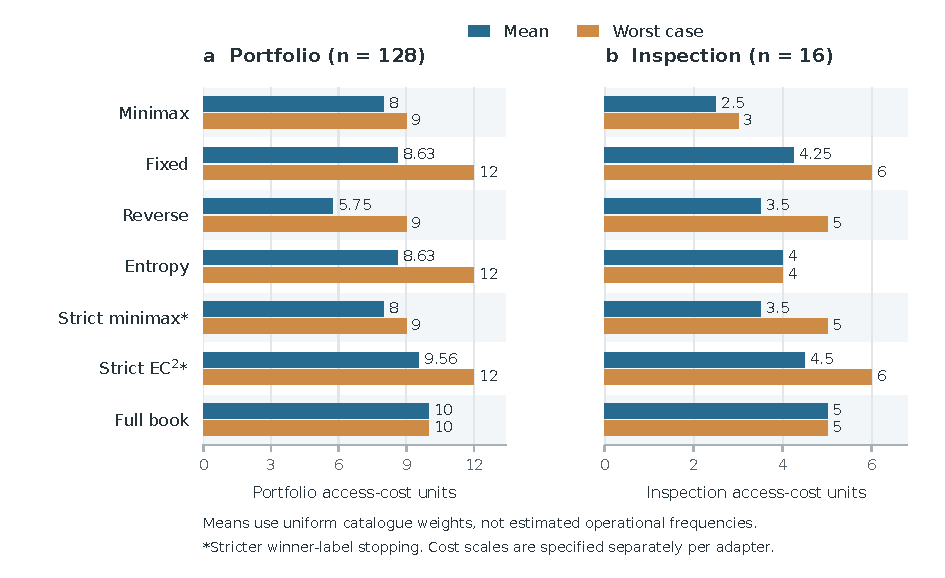
\includegraphics[width=\linewidth]{figures/portfolio_acquisition.pdf}
\caption{Mean and worst acquisition costs in the two constructed adapters. The financial reversed order matches the optimal worst cost while improving its mean. The industrial regional policy benefits from permitting overlapping acceptable actions. Access costs are adapter-specific and measure neither wall-clock speed nor financial return.}\label{fig:portfolioacquisition}
\end{figure}

\subsection{Independent checks and model-coverage boundaries}
The exact risk tests cover 504 single-distribution cases, 2910 convex-hull cases, 13750 mixture-grid lower comparisons and 960 invariance checks. They reject fourteen invalid numeric inputs and nineteen altered certificates. An additional floating linear-program diagnostic agrees in 95 cases to maximum absolute error $4.45\times10^{-16}$; this diagnostic is not the basis of the exact certificates.

Exhaustive decision-region checks cover 87040 small model tables and 314368 posterior states, including empty, overlapping and incompatible acceptable sets. Another 776 certificates, 768 policy paths, 28 tampering cases and 35 input or guard cases check the implementation. These finite tests complement the preservation and Bellman arguments; they do not replace their hypotheses.

The independent end-to-end verifier reconstructs all 128 current books, 384 cash constraints and 768 loss vectors directly from the fixed protocol. It checks the corresponding rational upper and lower risk witnesses without invoking the risk optimizer. It replays all 3696 policy paths across four financial settings and the industrial adapter, including 14756 passive observations, model identities, receipt times, query costs and terminal action sets. A separately implemented tuple-set Bellman recursion checks 16593 states and the reported worst-cost optima; a separate subset oracle verifies the complete-record references. Every saved path and reported mean passes these checks.

Boundary cases reject altered transcripts, foreign contract identities and premature observations, and preserve unresolved observational aliases. An explicit noncoverage example gives the same visible record a different true action outside the catalogue: the internal certificate remains valid for its model while its action is wrong for the omitted reality. This is the precise limitation of exact finite-model verification. Neither an exhaustive catalogue calculation nor an exact risk witness establishes external scenario coverage, calibrated probabilities or trustworthy record provenance.
\FloatBarrier


\subsection{Mean-cost refinement with an unchanged worst-case guarantee}\label{sec:budgetresults}
The five saved catalogues and their risk scores are held fixed. All use uniform record weights; only the constructed six-record counterexample uses a nonuniform prior. For each of the five catalogues, each policy is replayed on every record, at the minimum worst cap and at caps one and two units larger. ``Local'' below means worst-then-mean refinement at every posterior; ``budget'' solves \eqref{eq:budgetbellman}. Both retain the original acceptable-action target, unlike the earlier strict-label baselines.

\begin{table}[!htbp]\centering\small
\caption{Exact catalogue mean and achieved worst acquisition cost at the minimum root cap. Minimax uses the original query-index tie break; local and budget optimize a secondary mean objective. The inspection reverse policy ($\dagger$) exceeds its minimum cap three. Cost units are specified separately by each adapter.}\label{tab:budgetprimary}
\begin{tabular}{@{}l*{8}{@{\hspace{7pt}}r}@{}}
\toprule
& \multicolumn{2}{c}{Minimax} & \multicolumn{2}{c}{Reverse} & \multicolumn{2}{c}{Local} & \multicolumn{2}{c}{Budget} \\
\cmidrule(lr){2-3}\cmidrule(lr){4-5}\cmidrule(lr){6-7}\cmidrule(lr){8-9}
Model $(\epsilon,K)$ & Mean & Worst & Mean & Worst & Mean & Worst & Mean & Worst \\
\midrule
Portfolio $(2,25)$ & $8$ & $9$ & $23/4$ & $9$ & $45/8$ & $9$ & $45/8$ & $9$ \\
Portfolio $(0,25)$ & $8$ & $9$ & $25/4$ & $9$ & $97/16$ & $9$ & $97/16$ & $9$ \\
Portfolio $(6,25)$ & $8$ & $9$ & $23/4$ & $9$ & $45/8$ & $9$ & $45/8$ & $9$ \\
Portfolio $(2,15)$ & $55/8$ & $9$ & $43/8$ & $9$ & $21/4$ & $9$ & $21/4$ & $9$ \\
Inspection & $5/2$ & $3$ & $7/2$ & $5^{\dagger}$ & $5/2$ & $3$ & $5/2$ & $3$ \\
\bottomrule
\end{tabular}

\end{table}
The primary portfolio mean decreases from $8$ to $45/8=5.625$ at unchanged worst cost nine, below reversed order's $23/4=5.75$. This is a $19/64$ reduction of the original synthetic mean, not an estimate of monetary savings or execution latency. Local refinement ties the global optimum at the minimum cap in all five catalogues. The six-record example demonstrates why this agreement need not hold generally: exhaustive enumeration of its 64 nonredundant trees confirms means $13/4$ and $25/8$ at the same worst cost four.

\begin{table}[!htbp]\centering\small
\caption{Expected-cost frontier for the portfolio control $\epsilon=2$, $K=15$. The risk limit stays fixed; only the acquisition cap changes.}\label{tab:budgetfrontier}
\begin{tabular}{@{}rrr@{}}
\toprule
Allowed budget & Optimal mean & Achieved worst \\
\midrule
$9$ & $21/4$ & $9$ \\
$10$ & $73/16$ & $10$ \\
$11$ & $73/16$ & $10$ \\
\bottomrule
\end{tabular}

\end{table}
At $K=15$, raising the cap from nine to ten reduces the optimal mean from $21/4$ to $73/16$. Cap eleven provides no further improvement: the attaining policy still has worst cost ten. These larger-cap policies solve constrained expected acquisition, rather than the original minimax objective.

Independent small-table checks cover 8192 models, 262144 state--budget pairs, 65536 local-refinement states and 144 realized paths, with sixteen invalid-input and two guard-failure checks. A separate tuple-posterior verifier imports neither planner and checks all 6360 saved benchmark paths, 12449 passive observations and 41032 dynamic-program states; sixteen tampered records are rejected. It reconstructs queries, receipts, compatible sets, actions, exact weighted means and budget compliance. The prior risk calculation is inherited through its verified output hash; no new risk fitting or market calibration is performed.

\subsection{Revision checks and model-bound forecast records}\label{sec:renewalresults}
Executed checks cover 2016 renewal contracts, of which 674 pass the sufficient
gate, and 1462 exact allowed score realizations for the passing contracts.
Another 180 finite risk revisions satisfy the sensitivity bound, and twelve
two-loss cases attain its clipped probability term. Twelve event or binding
rejections and nine bound, payload or identity rejections exercise late
corrections, changed vintages, backward cutoffs and altered claims. These are
constructed finite checks accompanying the derivations; they are not a measured
renewal rate for real investment decisions.

The empirical snapshot driver applies the same versioned contract to the primary exchange-rate forecasts. At the declared as-of date 23 December 2025, it constructs one shared snapshot from 6909 source-date records and eight distinct currency/horizon contracts. Each target names the origin, currency and number of future observed intervals. The output stores the source-vintage identity, parameter digest, prefix cutoff, variance state and decimal and binary64-hex forecast values. It is a forecast record, not an acceptable-action or rounding certificate.

All sixteen quantile/CVaR values and sixteen associated variance-state values agree exactly with the archived primary forecasts. Suffix perturbation and truncation preserve the retained-prefix result, while eight altered forecast, target, cutoff or vintage cases and three invalid-date cases are rejected. The replay assigns event-date ordinal values to both clocks under an explicit same-day availability assumption; it does not claim those were measured historical receipt times. Moving the forecast origin changes its target and requires a fresh record rather than renewal of an old outcome claim.

\subsection{Held-out risk forecasts on reference-rate data}\label{sec:ecbresults}
\begin{table}[!htbp]\centering\small
\caption{Mean held-out FZ0 score on the 2020--2025 ECB-based log-loss targets; smaller is better. Fast and slow use half-lives 20 and 120. Multi is the predeclared equal-weight variance combination. Selected uses the weight $w$ chosen on completed 2010--2019 outcomes. Results are descriptive and losses share temporal observations.}\label{tab:ecbrisk}
\begin{tabular}{lrrrrrrrr}
\toprule
Currency & $h$ & Raw HS & Fast & Slow & Primary & Selected & $w_{\rm sel}$ & $n$ \\
\midrule
USD & 1 & 0.4082 & 0.2646 & 0.3696 & 0.3132 & 0.3400 & $1/4$ & 1537 \\
USD & 5 & 1.3960 & 1.1769 & 1.3727 & 1.2819 & 1.2819 & $1/2$ & 1533 \\
GBP & 1 & 0.1657 & 0.0852 & 0.1631 & 0.1149 & 0.1001 & $3/4$ & 1537 \\
GBP & 5 & 1.0702 & 1.0114 & 1.1112 & 1.0474 & 1.0809 & $1/4$ & 1533 \\
JPY & 1 & 0.4088 & 0.2981 & 0.3769 & 0.3148 & 0.3148 & $1/2$ & 1537 \\
JPY & 5 & 1.2001 & 1.0914 & 1.1438 & 1.0631 & 1.0562 & $3/4$ & 1533 \\
CHF & 1 & -0.0332 & -0.1556 & -0.0770 & -0.1368 & -0.1565 & $3/4$ & 1537 \\
CHF & 5 & 0.7325 & 0.7539 & 0.6994 & 0.6711 & 0.6711 & $1/2$ & 1533 \\
\bottomrule
\end{tabular}

\end{table}
The primary multiple-scale filter improves mean held-out FZ0 score over raw historical simulation in all eight currency--horizon comparisons (Table~\ref{tab:ecbrisk}). However, the fast single-scale filter scores better than the primary combination in six of eight. Its exceptions are JPY and CHF at horizon five. The development-selected family beats the raw control in seven of eight comparisons and is worse on GBP at horizon five. Selecting a variance mixture on past scores therefore does not guarantee the best future mixture or improve every future comparison.

The result is a positive financial forecasting comparison for temporal normalization against the declared raw historical control. It is not evidence that two scales are generally preferable to one, that the chosen grid is optimal, or that the recurrent trace network forecasts exchange rates. No market-return or investment-allocation performance is measured. The full candidate archive retains the weights that were not selected as well as the primary and control forecasts.

\begin{table}[!htbp]\centering\small
\caption{Held-out upper-VaR exceedance percentages for the same forecasts. The nominal tail probability is $2.5\%$. Frequencies alone do not establish conditional coverage; five-interval targets overlap.}\label{tab:ecbcoverage}
\begin{tabular}{lrrrrrr}
\toprule
Currency & $h$ & Raw HS & Fast & Slow & Primary & Selected \\
\midrule
USD & 1 & 3.90 & 2.54 & 3.32 & 3.19 & 3.19 \\
USD & 5 & 4.04 & 3.07 & 3.98 & 3.59 & 3.59 \\
GBP & 1 & 2.73 & 2.80 & 2.99 & 2.99 & 2.80 \\
GBP & 5 & 3.46 & 3.39 & 3.72 & 3.65 & 3.72 \\
JPY & 1 & 2.73 & 2.47 & 2.60 & 2.21 & 2.21 \\
JPY & 5 & 3.65 & 2.35 & 3.00 & 2.54 & 2.48 \\
CHF & 1 & 3.06 & 2.67 & 2.93 & 2.86 & 2.86 \\
CHF & 5 & 3.72 & 3.39 & 3.46 & 3.33 & 3.33 \\
\bottomrule
\end{tabular}

\end{table}
The primary filter's exceedance fractions range from approximately $2.21\%$ to $3.65\%$ across the eight targets. Seven are above the nominal $2.5\%$; JPY at horizon one is below it. Its mean expected-shortfall identification residual is positive in six comparisons and slightly negative in two. For USD at horizon five, the residual is approximately $0.502$ percentage-log-loss units and the exceedance fraction is $3.59\%$. Thus a better joint score than the raw historical control does not establish complete risk calibration. Table~\ref{tab:ecbcoverage} and the retained yearly summaries make that limitation measurable.

\begin{figure}[!htbp]\centering
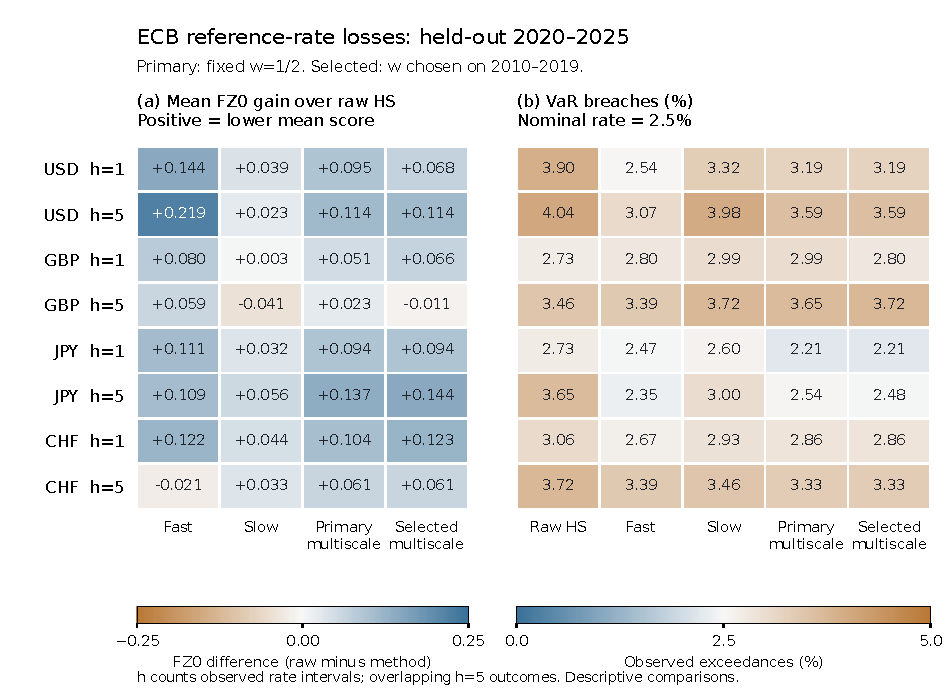
\includegraphics[width=\linewidth]{figures/ecb_risk_forecasts.pdf}
\caption{Gabriel calculations based on ECB reference rates. Left: paired mean-score improvement relative to raw historical simulation; positive values favor the filter. Right: upper-VaR exceedance percentages relative to the nominal $2.5\%$ tail. Forecast accuracy and empirical exceedance behavior are separate diagnostics. No transaction prices or investment returns are evaluated.}\label{fig:ecbrisk}
\end{figure}

Independent replay reconstructs all 325728 archived candidate VaR/CVaR pairs, including eligible predictions and candidates outside the reporting windows. It uses a separate extended-precision recurrence and sorted-tail integration in final loss units. Maximum absolute discrepancies are below $3.13\times10^{-13}$ for VaR and $2.70\times10^{-13}$ for CVaR, within the declared $10^{-10}$ absolute and relative tolerance. All 320 development, aggregate-test and yearly metric records and all eight model selections agree. The 61400 reported held-out forecast pairs are a subset of that archive.

Another 150 finite-distribution checks compare the tail formula with exact rational reference values. Three prefix cutoffs, each subjected to future-value perturbation and suffix removal, leave the corresponding earlier forecasts bitwise unchanged. Sixteen selection rechecks confirm that changes after the development boundary do not change its chosen weights. These checks support implementation and causal indexing. They are not directed-rounding proofs for the logarithms and variances, nor do they reconstruct unavailable historical data vintages.


\subsection{Maturity, correction and calibration-accounting checks}\label{sec:adaptivematurityresults}
The target-maturity implementation is checked against a separate explicit-history selector and rational controller replay on 160 constructed histories. The executed checks comprise 7734 snapshot comparisons, 30417 lane-state comparisons, 7734 retained-snapshot reconstructions and 3815 complete-prefix equivalence checks. Duplicate issues and receipts are idempotent; nineteen invalid-input cases are rejected. Delayed endpoints, overlapping targets, source corrections and tied timestamps are included. A clipped-update counterexample confirms that replay order matters.

The concrete financial replay consumes all 1480 primary forecasts whose origins and endpoints both fall in the 2026 extension. Each record binds its original quantile, expected shortfall, controller state, source digest and protocol. Its required outcome records are the currency rates at the origin and endpoint. Event and receipt clocks use observed-record indices under the declared same-day, current-vintage convention. Each lane begins from its archived first retained state; this bridge checks the 2026 transitions rather than reconstructing the preceding years of learning.

Every target remains pending when issued. At maturity, all 1480 exceedance bits, preupdate states, postupdate states and issue-state comparisons match the saved experiment exactly. Controller states use integer multiples of $1/800$, with increments $+39$ for an exceedance and $-1$ otherwise, clipped to $[-800,800]$. Eight isolated synthetic final-endpoint corrections each replace one active score, preserve issued forecasts, and change the affected current-information replay state. A separate direct integer fold reproduces that state. Earlier snapshots reconstruct at their original operation prefixes. These constructed corrections are not observed ECB revision events.

Independent rational checks of Proposition~\ref{prop:adaptiveaccounting} cover 5120 parameterized binary paths, 40960 updates and 184320 finite windows with their actual initial states. Further checks cover 1458 upper-envelope cases, 729 two-sided envelope cases, saturation extremes, zero-rate exclusion from the divided identity and stale-feedback failure. The forty-step counterexample returns exactly to state zero with breach frequency $1/40$, while its displayed binary64 mean ES residual is approximately $39.04758$. These tests complement the algebraic derivation; they do not convert the exponential illustration into an interval proof.

\subsection{Adaptive frequency feedback and joint risk accuracy}\label{sec:adaptiveresults}
The seven reported methods produce 143136 development pairs, 85960 retrospective pairs and 10360 pairs in the 2026 extension. They share respectively 20448, 12280 and 1480 currency--horizon--origin cases. The extension contains 187 completed one-interval targets and 183 five-interval targets per currency. At the source endpoint, another 24 contract targets remain pending and receive no fabricated outcome. The complete archive retains 868992 candidate pairs, including inherited base candidates, alternative scales and rates, and pending forecasts; these are not independent observations.

Development selection chooses $\eta=1/100$ for six contracts, zero for JPY at horizon one, and $1/20$ for CHF at horizon five. The selected static log scale is zero for five contracts, $1/5$ for GBP and JPY at horizon five, and $2/5$ for CHF at horizon five. All choices remain fixed in the later windows.

\begin{table}[!htbp]\centering\small
\caption{Mean joint risk-score differences from the unchanged fast FHS base. Negative differences favor the alternative. Static is the development-selected constant scale; primary uses rate $1/20$ in horizon lanes; selected chooses its rate only on 2010--2019. The later 2026 window is short and descriptive.}\label{tab:adaptivescore}
\begin{tabular}{@{}lrrrrr@{}}\toprule
Currency & $h$ & Fast FZ0 & $\Delta$ static & $\Delta$ primary & $\Delta$ selected\\\midrule
\multicolumn{6}{l}{\textit{Retrospective: 2020--2025}}\\
USD & 1 & 0.2646 & +0.0000 & +0.0226 & +0.0051\\
USD & 5 & 1.1769 & +0.0000 & -0.0052 & -0.0145\\
GBP & 1 & 0.0852 & +0.0000 & +0.0094 & +0.0033\\
GBP & 5 & 1.0114 & -0.0074 & -0.0057 & -0.0083\\
JPY & 1 & 0.2981 & +0.0000 & +0.0180 & +0.0000\\
JPY & 5 & 1.0914 & +0.0337 & +0.0195 & +0.0002\\
CHF & 1 & -0.1556 & +0.0000 & +0.0128 & +0.0035\\
CHF & 5 & 0.7539 & +0.1074 & +0.0027 & +0.0027\\
\midrule
\multicolumn{6}{l}{\textit{Temporal extension: 2026 through 25 September}}\\
USD & 1 & -0.0038 & +0.0000 & +0.0258 & +0.0034\\
USD & 5 & 0.7379 & +0.0000 & +0.0451 & +0.0072\\
GBP & 1 & -0.6498 & +0.0000 & +0.0285 & +0.0049\\
GBP & 5 & -0.0606 & +0.1966 & +0.0847 & +0.0481\\
JPY & 1 & -0.1650 & +0.0000 & +0.0024 & +0.0000\\
JPY & 5 & 0.5516 & +0.1332 & +0.0352 & +0.0234\\
CHF & 1 & -0.7755 & +0.0000 & +0.0232 & -0.0007\\
CHF & 5 & 0.0643 & +0.2365 & +0.0264 & +0.0264\\
\bottomrule\end{tabular}

\end{table}

The primary controller lowers the joint FZ0 score in two of eight retrospective comparisons, both at horizon five (USD and GBP). It improves the absolute breach-frequency discrepancy in five of eight. Thus even in that longer window, improving the frequency criterion does not imply improving the joint score. In the 2026 extension, the primary controller has a higher joint score in all eight comparisons. Frequency discrepancy improves for USD at both horizons, worsens for GBP and CHF at horizon five, and is unchanged in the remaining four.

The development-selected controller improves the joint score in two retrospective comparisons and one extension comparison, ties the unchanged JPY one-interval base through its zero rate, and loses the remainder. The selected static correction improves one retrospective joint score and none in the extension; it ties the base in its five zero-scale cases. The experiment therefore supplies no evidence for replacing the fast base with either tested adaptive scale rule as a generally better forecaster.

\begin{table}[!htbp]\centering\small
\caption{Exceedance counts in the 2026 extension, using the same retained targets for every column. At nominal $\beta=1/40$, the reference counts are $4.675$ for $n=187$ and $4.575$ for $n=183$. A difference of one breach is already about half a percentage point. Counts alone do not establish conditional calibration.}\label{tab:adaptivecounts}
\begin{tabular}{@{}lrrrrrr@{}}\toprule
Currency & $h$ & $n$ & Fast & Static & Primary & Selected\\\midrule
USD & 1 & 187 & 6 & 6 & 5 & 5\\
USD & 5 & 183 & 7 & 7 & 3 & 4\\
GBP & 1 & 187 & 5 & 5 & 5 & 4\\
GBP & 5 & 183 & 1 & 0 & 0 & 0\\
JPY & 1 & 187 & 2 & 2 & 2 & 2\\
JPY & 5 & 183 & 3 & 0 & 3 & 3\\
CHF & 1 & 187 & 6 & 6 & 6 & 6\\
CHF & 5 & 183 & 5 & 0 & 4 & 4\\
\bottomrule\end{tabular}

\end{table}

The horizon-lane controller scores better than its pooled counterpart on all four retrospective five-interval contracts and three of four extension contracts. At horizon one they coincide. This isolates a consequence of the feedback schedule under the fixed protocol, but does not rescue the broader adaptation claim. The unchanged equal-weight two-scale base itself scores better than the fast base on seven of eight extension targets, compared with two of eight in 2020--2025. That reversal emphasizes the period dependence of the rankings; the short extension cannot establish a new universal preference.

\begin{figure}[!htbp]\centering
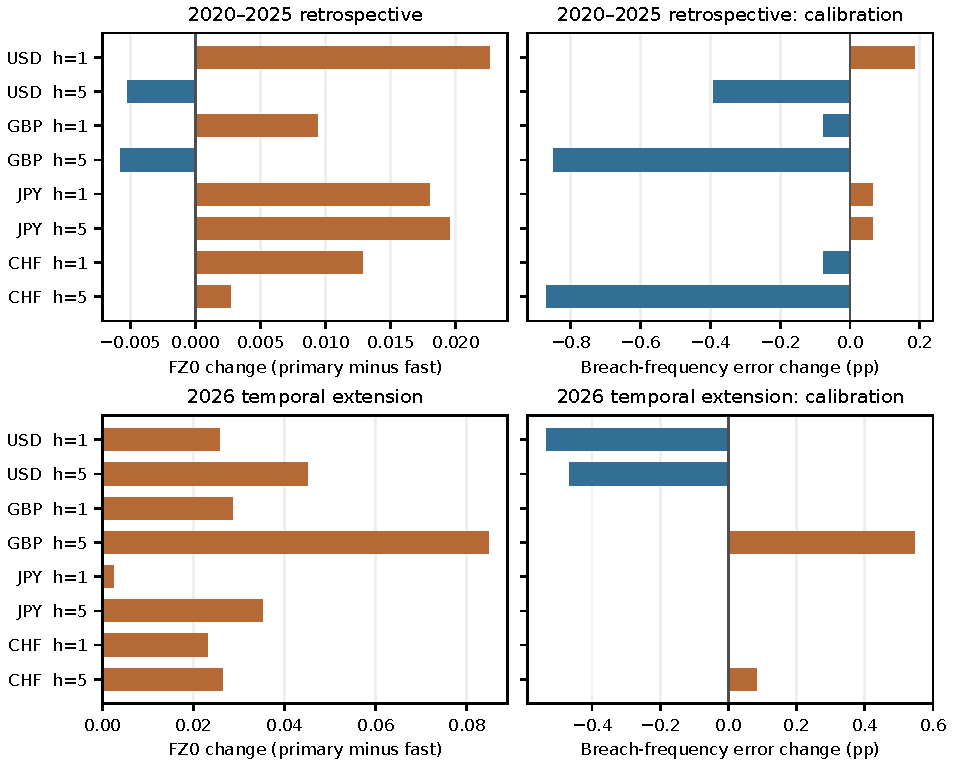
\includegraphics[width=0.98\textwidth]{figures/adaptive_risk_tradeoff.pdf}
\caption{Primary adaptive controller relative to its fast base. Negative joint-score changes are favorable; negative changes in absolute breach-frequency error are closer to the nominal $2.5\%$. The two axes measure distinct properties, as the sign disagreements demonstrate. Values are Gabriel calculations from the unchanged ECB reference-rate snapshot.}\label{fig:adaptivetradeoff}
\end{figure}

No historical candidate path reaches the controller bounds, so all recorded projection increments are zero. This observed fact permits exact state-only frequency accounting on those paths, but establishes no bound on future projections. The new adverse joint-score result therefore cannot be attributed to saturation in this experiment. The binary feedback objective and fixed within-pair severity ratio provide a precise reason why frequency correction need not improve joint risk accuracy; the experiment does not isolate every possible source of forecast error.

Independent verification reconstructs 271560 adaptive and 271560 static forecast pairs. Their values and all exact state, hit and projection arrays agree with the producer. It reuses the checksums and independent replay of 325728 unchanged parent pairs, and separately reconstructs 144 pending parent pairs through sorted final-unit tails. All 1672 metric records and 1640 exact accounting records are reproduced; maximum metric and selection discrepancies are below $3.56\times10^{-15}$ and $4.67\times10^{-15}$ respectively. Six suffix perturbation or truncation variants at three cutoffs preserve earlier outputs, and sixteen development-selection rechecks preserve chosen parameters. Additional tests exercise target timing, both clipping boundaries, zero rates and invalid inputs. These are implementation and causal-index checks, with no directed-rounding or conditional-calibration claim.
\FloatBarrier

\subsection{Severity objective and correction identities}
Exact rational checks evaluate 3072 weighted-state prefixes and their same-input fading identity, 9216 constrained optima, 193536 reciprocal-coordinate variational inequalities, 3840 fixed-position corrections and 9216 cap perturbation bounds. A further 288 discrete and 45 continuous tail-functional cases check the quantile-envelope relationship. Counterexamples distinguish normalized from raw residual balance, demonstrate loss of the weighted objective when the accumulator is clipped, and exhibit ES underestimation imposed by a finite ratio cap. Nine alternating-regime cases verify that a correct historical optimizer can have worse next-step scores than a fixed ratio. The separate 999 binary64 score-decomposition illustrations have maximum discrepancy $2.85\times10^{-14}$ at tolerance $10^{-12}$. These finite checks accompany the derivations; they do not establish forecast calibration.

\subsection{Severity adaptation on observed exchange-rate losses}\label{sec:severitymarketresults}
Table~\ref{tab:severitymarket} reports every predeclared severity variant against its unchanged quantile-stream comparator. The primary severity memory of 125 observations worsens mean FZ0 relative to the fast base in all eight 2020--2025 contracts and improves only JPY at horizon five in 2026. Adding the same severity memory to the frequency-controlled quantile worsens the frequency-only pair in all eight contracts of both periods. Thus a separate severity state does not by itself establish a predictive gain on these observations.

The slower, predeclared 500-observation severity control improves six of eight fast-base comparisons in 2020--2025, but only one in 2026. The static severity ratio improves five and two respectively. The corresponding joint 500-observation variant improves the frequency-only pair in four and two cases; the static joint ratio improves six and two. These are distinct fixed comparisons, not a post-result selection of a winning memory length. In particular, small negative values displayed near zero are evaluated using unrounded scores in the saved summaries.

\begin{table}[htbp]\centering\small
\caption{Retrospective mean FZ0 differences with unchanged quantiles. $S_d$ changes only severity relative to the fast base; $J_d$ changes severity relative to the frequency-only pair. Subscript $d$ is the feedback half-life and ``fix'' denotes the development-fitted constant ratio. Negative differences favor the severity variant. All eight models remain in the saved results.}\label{tab:severitymarket}
\begin{tabular}{lrrrrrr}
\toprule
Contract & $\Delta S_{125}$ & $\Delta J_{125}$ & $\Delta S_{500}$ & $\Delta J_{500}$ & $\Delta S_{\rm fix}$ & $\Delta J_{\rm fix}$ \\
\midrule
\multicolumn{7}{l}{\textit{2020--2025, retrospective}} \\
USD, 1 & +0.0078 & +0.0057 & -0.0002 & +0.0005 & -0.0040 & -0.0016 \\
USD, 5 & +0.0336 & +0.0354 & -0.0073 & +0.0015 & -0.0275 & -0.0161 \\
GBP, 1 & +0.0057 & +0.0015 & +0.0013 & -0.0032 & -0.0025 & -0.0068 \\
GBP, 5 & +0.0163 & +0.0184 & -0.0059 & +0.0006 & -0.0214 & -0.0123 \\
JPY, 1 & +0.0073 & +0.0071 & -0.0003 & -0.0013 & +0.0020 & -0.0027 \\
JPY, 5 & +0.0271 & +0.0242 & +0.0022 & +0.0023 & -0.0095 & -0.0087 \\
CHF, 1 & +0.0107 & +0.0106 & -0.0033 & -0.0031 & +0.0268 & +0.0194 \\
CHF, 5 & +0.0100 & +0.0065 & -0.0143 & -0.0088 & +0.1049 & +0.1052 \\
\midrule
\multicolumn{7}{l}{\textit{2026 through 25 September, retrospective}} \\
USD, 1 & +0.0114 & +0.0094 & +0.0162 & +0.0158 & +0.0106 & +0.0074 \\
USD, 5 & +0.0216 & +0.0131 & +0.0295 & +0.0208 & +0.0173 & +0.0127 \\
GBP, 1 & +0.0051 & +0.0103 & +0.0024 & -0.0005 & -0.0002 & -0.0027 \\
GBP, 5 & +0.0168 & +0.0034 & +0.0527 & +0.0284 & +0.0472 & +0.0304 \\
JPY, 1 & +0.0131 & +0.0269 & +0.0055 & +0.0144 & +0.0192 & +0.0188 \\
JPY, 5 & -0.0019 & +0.0008 & -0.0206 & -0.0203 & -0.0179 & -0.0262 \\
CHF, 1 & +0.0073 & +0.0090 & +0.0032 & +0.0032 & +0.0518 & +0.0309 \\
CHF, 5 & +0.0272 & +0.0095 & +0.0288 & +0.0166 & +0.2289 & +0.2082 \\
\bottomrule
\end{tabular}

\end{table}

{\clubpenalty=10000
Because the severity adapter leaves its supplied quantiles unchanged, its exceedance counts exactly equal those of that quantile stream. Any score change in a matched comparison comes from the ES component. No ratio cap activates on any archived market path. The primary memory's negative score results therefore occur within the unconstrained ratio range. Raw and quantile-normalized residuals are both retained; neither a favorable residual nor a score difference is treated as a proof of conditional calibration.\par}

The eight models contribute 98240 forecast pairs over 12280 distinct currency--horizon targets in 2020--2025 and 11840 pairs over 1480 targets in 2026. Development has 20448 target cases and 163584 fitted or adaptive pairs. The model copies do not enlarge the number of observed outcomes. The same 24 final pending targets remain unscored. Static arrays explicitly mark their fitting rows and the date from which their fitted ratios were available.

\subsection{Controlled severity changes and error attribution}\label{sec:severitysyntheticresults}
The known-law study evaluates 320 case--latency--replication combinations and retains 8640 model/window metric records, including the oracle. Table~\ref{tab:severitysynthetic} gives paired differences in analytically integrated conditional expected FZ0 over all scored origins. The intervals reflect variation across independently generated paths, rather than treating successive outcomes within a path as independent forecast comparisons.

\begin{table}[htbp]\centering\small
\caption{Synthetic conditional expected-score differences: mean $\pm$ marginal 95\% Monte Carlo interval half-width across 32 paired replications. Each row uses all scored origins. Negative values favor the adaptive variant. These constructed laws and references are specified in Table~\ref{tab:severitydgps}; ``Freq'' is the frequency-only pair.}\label{tab:severitysynthetic}
\begin{tabular}{lrllll}
\toprule
Generating process & Delay & $S_{125}-$base & $S_{125}-S_{\rm fix}$ & $J_{125}-$Freq & $J_{125}-J_{\rm fix}$ \\
\midrule
Stationary & 1 & $+0.008\,\pm\,0.001$ & $+0.007\,\pm\,0.001$ & $+0.003\,\pm\,0.002$ & $+0.007\,\pm\,0.001$ \\
 & 5 & $+0.008\,\pm\,0.001$ & $+0.007\,\pm\,0.001$ & $+0.003\,\pm\,0.001$ & $+0.005\,\pm\,0.001$ \\
\addlinespace[2pt]
Sustained shift & 1 & $-0.413\,\pm\,0.005$ & $-0.413\,\pm\,0.022$ & $-0.264\,\pm\,0.023$ & $-0.321\,\pm\,0.029$ \\
 & 5 & $-0.412\,\pm\,0.005$ & $-0.413\,\pm\,0.022$ & $-0.306\,\pm\,0.013$ & $-0.337\,\pm\,0.021$ \\
\addlinespace[2pt]
Recurrent shift & 1 & $-0.253\,\pm\,0.008$ & $-0.037\,\pm\,0.010$ & $-0.158\,\pm\,0.013$ & $-0.029\,\pm\,0.007$ \\
 & 5 & $-0.251\,\pm\,0.008$ & $-0.035\,\pm\,0.010$ & $-0.172\,\pm\,0.009$ & $-0.033\,\pm\,0.008$ \\
\addlinespace[2pt]
Exponential tail & 1 & $-0.398\,\pm\,0.009$ & $-0.397\,\pm\,0.019$ & $-0.258\,\pm\,0.018$ & $-0.305\,\pm\,0.024$ \\
 & 5 & $-0.398\,\pm\,0.009$ & $-0.398\,\pm\,0.019$ & $-0.304\,\pm\,0.009$ & $-0.336\,\pm\,0.020$ \\
\addlinespace[2pt]
Low quantile & 1 & $-0.910\,\pm\,0.005$ & $-0.280\,\pm\,0.017$ & $-0.244\,\pm\,0.031$ & $-0.284\,\pm\,0.035$ \\
 & 5 & $-0.910\,\pm\,0.005$ & $-0.279\,\pm\,0.017$ & $-0.294\,\pm\,0.014$ & $-0.266\,\pm\,0.017$ \\
\addlinespace[2pt]
\bottomrule
\end{tabular}

\end{table}

Under the stationary bounded law, the base pair equals the true conditional pair. Estimating an additional ratio introduces error: at latency one, the primary severity state adds approximately $0.008$ expected score. Under sustained tail change, its mean conditional excess score over the oracle falls from $0.457$ for the fixed base to $0.045$; the paired score reduction is $0.413$ with interval $[0.407,0.418]$ in improvement units. This comparison averages the declared pre- and post-change scoring intervals and is not a claim about an arbitrary change time. The recurrent and exponential-tail cases also favor primary severity adaptation over their base and fitted static-ratio controls. Figure~\ref{fig:severityresponse} shows one retained path together with aggregate comparisons.

\begin{figure}[htbp]\centering
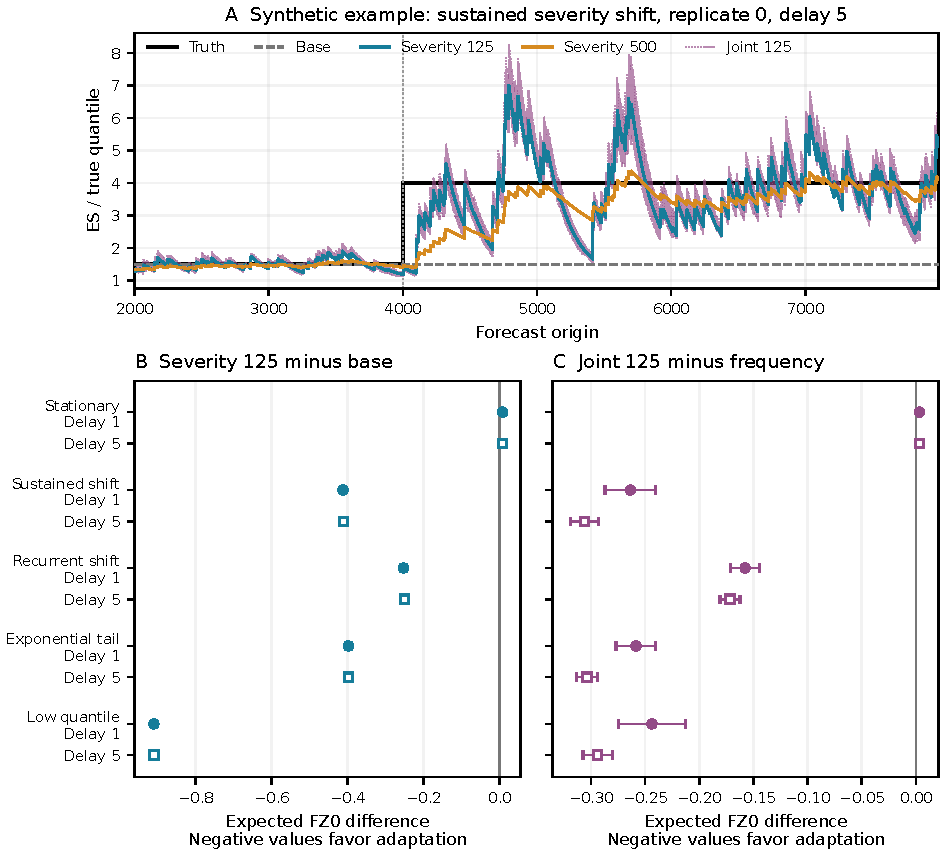
\includegraphics[width=\linewidth]{figures/severity_response.pdf}
\caption{Controlled severity response and paired expected-score comparisons. The path panel is the saved replication-zero sustained-change example with latency five, not an observed market trajectory. The two aggregate panels use all 32 replications per indicated case and latency; marginal 95\% intervals quantify Monte Carlo uncertainty under those generating laws.}\label{fig:severityresponse}
\end{figure}

\begin{table}[htbp]\centering\small\setlength{\tabcolsep}{4pt}
\caption{Mean conditional excess-score decomposition over all scored synthetic origins and replications. $C_Q$ is quantile misspecification and $C_E$ severity mismatch at that quantile, as in \eqref{eq:severitydecomposition}. The oracle has both terms zero.}\label{tab:severitydecomposition}
\begin{tabular}{lrrrrrrrrr}
\toprule
Process & Delay & \multicolumn{2}{c}{Base} & \multicolumn{2}{c}{Freq} & \multicolumn{2}{c}{$S_{125}$} & \multicolumn{2}{c}{$J_{125}$} \\
 & & $C_Q$ & $C_E$ & $C_Q$ & $C_E$ & $C_Q$ & $C_E$ & $C_Q$ & $C_E$ \\
\midrule
Stationary & 1 & 0.000 & 0.000 & 0.010 & 0.008 & 0.000 & 0.008 & 0.010 & 0.011 \\
 & 5 & 0.000 & 0.000 & 0.009 & 0.007 & 0.000 & 0.008 & 0.009 & 0.011 \\
Sustained shift & 1 & 0.000 & 0.457 & 0.004 & 0.317 & 0.000 & 0.045 & 0.004 & 0.054 \\
 & 5 & 0.000 & 0.457 & 0.003 & 0.355 & 0.000 & 0.045 & 0.003 & 0.050 \\
Recurrent shift & 1 & 0.000 & 0.343 & 0.009 & 0.254 & 0.000 & 0.090 & 0.009 & 0.096 \\
 & 5 & 0.000 & 0.343 & 0.007 & 0.267 & 0.000 & 0.092 & 0.007 & 0.096 \\
Exponential tail & 1 & 0.000 & 0.457 & 0.005 & 0.327 & 0.000 & 0.059 & 0.005 & 0.068 \\
 & 5 & 0.000 & 0.457 & 0.004 & 0.367 & 0.000 & 0.059 & 0.004 & 0.064 \\
Low quantile & 1 & 0.139 & 0.948 & 0.004 & 0.295 & 0.139 & 0.037 & 0.004 & 0.051 \\
 & 5 & 0.139 & 0.947 & 0.004 & 0.342 & 0.139 & 0.038 & 0.004 & 0.049 \\
\bottomrule
\end{tabular}

\end{table}

The underestimated-quantile case distinguishes the two error sources. At latency one, severity-only adaptation retains a mean quantile cost of $0.139$ while reducing its severity cost to $0.037$. The joint variant reduces the quantile cost to $0.004$ and has severity cost $0.051$, for a smaller total error. Correcting severity at a wrong quantile thus does not remove the quantile penalty. The other correctly specified base-quantile cases have zero such penalty before frequency adaptation; the frequency learner itself can add quantile estimation error. The largest pointwise numerical discrepancy in the implemented decomposition is $8.89\times10^{-16}$. No emitted ratio cap activates in the generated benchmark paths; separate stress tests exercise that branch.

These cases establish that the severity mechanism can respond to the stipulated changes and that its two error sources are measurable when the law is known. Their deliberately under-responsive base after a tail shift does not represent a competitive empirical forecaster. Neither these gains nor the oracle information is transferred to the financial comparisons.

\subsection{Independent severity verification and maturity replay}
An independent implementation reconstructs all eight market contracts and 192 metric records across models and periods. It regenerates all 320 synthetic case--latency--replication runs, including 23,040,000 model-pair array entries and 8640 model/window metric records. Of these, 720000 pair entries belong to the fully archived replication-zero traces. Counts include oracle entries and explicitly marked pre-fit static values, rather than independent observations. Long-double recurrence and independent analytic tail integration check the binary64 producer; 360 explicit weighted-sum cases check the recurrence against its finite history. Maximum forecast or state discrepancy is below $3.32\times10^{-13}$, with market and synthetic metric discrepancies below $2.32\times10^{-14}$ and $3.81\times10^{-14}$ respectively. Declared comparisons use absolute and relative tolerances $10^{-10}$. The archived market arrays contain 434496 model pairs, including marked pre-fit static values. Independent aggregation additionally checks 270 synthetic method summaries, 2640 paired comparisons and 4800 Monte Carlo intervals, with maximum discrepancy below $6.16\times10^{-16}$.

Future-outcome perturbations begin with targets that are still unavailable at the tested issue time, verifying receipt causality rather than only origin-date ordering. Static fits are checked on their prescribed fitting masks and interpreted as available only after fitting. Large-shock tests distinguish the correct uncapped sufficient statistic from an incorrectly clipped state and exercise cap recovery. Twenty-four unavailable-suffix variants, four maturity cases, two pending-target cases, four static-fit causality rechecks, 144 analytic positive-part cases and ten rejected invalid inputs pass. These numerical checks support the implemented recursion, known-law integration and evaluation indexing; they are not interval-arithmetic or population-calibration certificates.

\paragraph{Maturity and correction checks.}
The severity replay covers 1480 distinct currency--horizon targets with both endpoints in 2026. Applying the two primary quantile streams gives 2960 forecast--target pairs. The 24 distinct boundary targets pending at the imported start-of-2026 checkpoint contribute another 48 pairs, for 3008 immutable issued records in total. Every retained issue-time raw accumulator, preupdate accumulator, postupdate accumulator and severity response agrees with the producer's saved binary64 values; the maximum observed discrepancy is zero. The 48 boundary pairs also reproduce their pre- and postupdate states. These are implementation comparisons under imported checkpoints, not exact-real arithmetic certificates.

Sixteen isolated synthetic final-price revisions replace one feedback record each. They preserve the active target count, kernel weights and all issued forecasts. The corrected raw state agrees with direct replay; the affine final-position correction differs by at most $2.23\times10^{-16}$. Every original snapshot remains unchanged and reconstructs at its retained accepted-operation prefix.

A further 144 synthetic score substitutions cover the first, middle and last maturity positions, with increased scores, scores reduced to one, and scores large enough to activate the emitted-ratio cap. The direct correction and full replay agree within $2.49\times10^{-13}$ in raw state; emitted ratios and cap flags agree under the declared checks. Each market-window replay contains 188 sequential updates. The correction evaluates one power and a fixed arithmetic expression for the changed score, preserving the normalization of the existing kernel. These tests use absolute and relative tolerances of $10^{-11}$.

Separate helper checks compare 1024 finite sequences with exact rational reference calculations, with a largest binary64 discrepancy below $7.11\times10^{-15}$ at tolerances $10^{-12}$. Ten invalid-input cases are rejected. The algebraic correction identity supplies the general result; finite numerical checks assess this implementation and do not establish directed-rounding guarantees.



\subsection{Joint aggregation on previously unscored assets}\label{sec:aggregateresults}

The asset-transfer comparison contains 1721 common forecast-origin dates from 2 January 2020 through 18 September 2026, giving 13768 currency--horizon cases. The primary adaptive pool has mean FZ0 score $0.68518$. It improves on uniform arithmetic pooling by $0.01379$ score units and on fitted transformed pooling by $0.00423$, but loses to fitted arithmetic pooling by $0.00196$ and to the development-selected expert by $0.00506$. These are paired additive score differences, not percentage gains or trading returns.

\begin{table}[htbp]\centering\small
\caption{Primary adaptive pool minus each frozen comparator, equally weighted over eight contracts and common dates. Negative differences favor the primary. Upper limits are one-sided 95\% percentile limits from 5000 paired circular block resamples at each length $L$; they are approximate historical dependence diagnostics. ``Better/8'' counts negative contract means.}\label{tab:aggregatebootstrap}
\resizebox{\linewidth}{!}{\begin{tabular}{lrrrr}\toprule
Comparator & $\Delta$ & Upper 95\%, $L=20$ & Upper 95\%, $L=60$ & Better/8\\\midrule
Fitted arithmetic pool & 0.00196 & 0.01625 & 0.01714 & 6\\
Uniform arithmetic pool & -0.01379 & -0.00524 & -0.00378 & 7\\
Development-best expert & 0.00506 & 0.02804 & 0.02886 & 4\\
Fitted transformed pool & -0.00423 & 0.01564 & 0.01554 & 5\\
\bottomrule\end{tabular}
}
\end{table}

The prespecified conjunctive superiority criterion is not met. Only the uniform arithmetic comparison has a negative upper limit at both block lengths: $-0.00524$ for $L=20$ and $-0.00378$ for $L=60$. All three other comparisons have positive upper limits. The common-date resampling preserves cross-currency and cross-horizon dependence within each sampled vector and local dependence within a block. It does not establish stationarity, adequate block length for every market episode, or finite-sample coverage under arbitrary nonstationarity. The passing uniform-pool comparison therefore supports a narrower historical comparison; it does not replace the failed four-comparator criterion.

The contract results explain why a count of wins would misstate the aggregate result. The primary improves six of eight contract means against fitted arithmetic pooling, but its AUD five-interval loss is $0.04810$, larger than its greatest gain of $0.02729$ on SEK at the same horizon. It beats the development-selected expert on four contracts and loses on four, with the largest loss $0.03802$ on NOK at horizon five. Against uniform arithmetic pooling it improves seven contracts; AUD at horizon five is again the exception. Figure~\ref{fig:aggregatecomparison} retains all four comparator profiles.

\begin{table}[htbp]\centering\small
\caption{Common-date contract scores. The primary is the causal adaptive transformed pool with $c=0.1$; each difference subtracts the named comparator from that primary.}\label{tab:aggregatecontracts}
\resizebox{\linewidth}{!}{\begin{tabular}{llrrrr}\toprule
Currency & $h$ & Primary score & $\Delta$ fitted arithmetic & $\Delta$ uniform arithmetic & $\Delta$ best expert\\\midrule
AUD & 1 & 0.34327 & 0.00281 & -0.02455 & -0.00236\\
AUD & 5 & 1.27732 & 0.04810 & 0.00842 & 0.02787\\
CAD & 1 & 0.07209 & -0.00299 & -0.01803 & 0.00599\\
CAD & 5 & 1.10910 & -0.00111 & -0.01342 & -0.01137\\
NOK & 1 & 0.51640 & -0.00118 & -0.01172 & 0.02540\\
NOK & 5 & 1.47367 & -0.00146 & -0.04168 & 0.03802\\
SEK & 1 & -0.03951 & -0.00122 & -0.00474 & -0.01155\\
SEK & 5 & 0.72909 & -0.02729 & -0.00457 & -0.03154\\
\bottomrule\end{tabular}
}
\end{table}

The full retained model set prevents the candidate family from defining its own favorable comparison. Fast FHS scores $0.68266$ and its 500-observation severity adjustment scores $0.67883$, both below the primary. The faster adaptive settings $c=0.3$ and $c=1$ score $0.69202$ and $0.69683$. Uniform transformed pooling scores $0.70262$, compared with $0.69897$ for uniform arithmetic pooling. Thus the convex coordinate system supplies a tractable joint objective without establishing that those coordinates produce the best empirical forecasts.

The transformed development fits have computed objective-to-lower-bound gaps no larger than $6.18\times10^{-9}$. This is a binary64 diagnostic accompanying the convex derivation, not a directed-rounding certificate. The arithmetic comparator retains the best feasible result from its nine declared starts; its nonconvex objective has no global-optimality claim. The observed forecast ranking is therefore distinct from the existence and uniqueness of a regularized empirical optimum.

\paragraph{Measured convexity gain.}
The primary's mean score reduction relative to the weighted average of its own experts' scores is $0.02266$. The logarithmic component contributes $0.00896$ and the hinge component $0.01370$. Every one of the 13768 retained primary cases has a total gain exceeding $10^{-12}$; the largest recomputed score-identity residual is $1.55\times10^{-14}$. This verifies the realized manifestation of the pointwise convexity identity. Its comparator is randomized expert selection with the same issue-time weights in expectation, rather than the best individual expert or arithmetic pooling. All five transformed methods' components are retained; none is selected after inspecting this diagnostic.

\begin{figure}[htbp]\centering
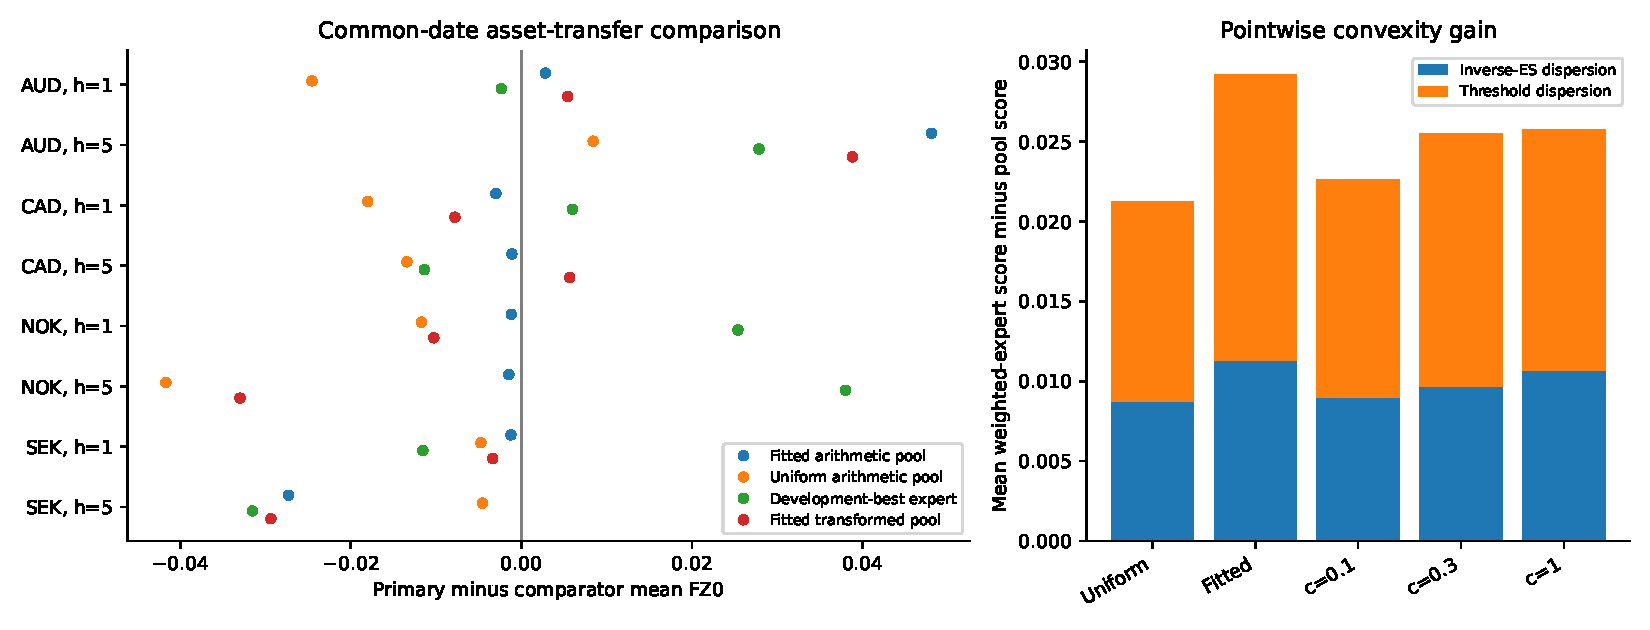
\includegraphics[width=\linewidth]{figures/aggregate_risk_comparison.pdf}
\caption{Left: primary-minus-comparator score differences for all eight contracts; negative values favor the primary. Right: mean pointwise convexity gain relative to the weighted expert-score average, decomposed into inverse-ES and threshold dispersion. The right panel's guaranteed comparison differs from each empirical reference on the left.}\label{fig:aggregatecomparison}
\end{figure}

Secondary windows preserve the temporal variation. On the 2020--2025 cases the primary-minus-fitted-arithmetic mean is $+0.00272$; on the 1464 cases within the common-date 2026 subset it is $-0.00247$. The corresponding differences against the development-selected expert are $+0.00631$ and $-0.00560$. Against fitted transformed pooling they are $-0.00464$ and $+0.00048$. These descriptive subdivisions do not select a new primary model or change the full-window criterion. The 16 additional matured one-interval cases beyond the common date window remain separately reported; they are not silently discarded from the archive. The producer also retains the complete 1480-case 2026 window.

The result is an implemented, causal joint aggregation mechanism with an explicit convexity gain, a unique regularized fitting target and a falsifiable competitive evaluation. Its complete prespecified empirical superiority claim fails on this asset extension. The one-source, shared-currency-factor and already examined calendar setting further limits transfer to independent markets or future observations.



\paragraph{Post-test mechanism diagnosis.}
A descriptive analysis retains every original outcome while measuring concentration and learning-rate history. Removing just the single most adverse shared origin, separately for each comparison, leaves the primary's mean deficit positive against fitted arithmetic pooling, the selected expert and fast FHS. The primary failure is therefore not attributable to one isolated date. This deletion diagnostic does not alter the reported benchmark or justify removing real tail events.

Across the 24 primary maturity lanes, gradient energy accumulated before 2020 accounts for 23.68--79.94\% of the final normalization. The final test step is 48.66--89.41\% of its initial test value. Weights continue changing, but the cumulative normalization permanently retains old gradients. These measurements motivate the controlled interventions in Section~\ref{sec:forgetting}. The saved market trajectories alone do not identify the causal effect of altering gradient memory. The additional experiments separate that intervention from resetting weights and from changing the step multiplier.

\subsection{Independent aggregation checks}
A separate implementation reconstructs decimal ECB rates, variance states and sorted historical tails in extended precision. It checks 325872 base forecast pairs, all 434496 expert pairs and 868992 archived model pairs, including the development and pending portions outside the primary test. The complete audit covers 102768 online updates, 704 metric records, every one of the 144 optimizer-start objectives and 20448 saved hinge-dual coefficients. The largest base forecast discrepancy is $8.13\times10^{-14}$ and the largest weight discrepancy $2.17\times10^{-15}$. The squared-gradient accumulator differs by at most $6.76\times10^{-11}$ in absolute value. These are independent floating-point recomputations, not interval certificates.

Sixteen future-suffix mutation or truncation checks leave all 48 static fitting input arrays bitwise unchanged and reproduce the selected individual experts. The audit reconstructs the primary choice from the eight retained development scores. It also checks 271440 Jensen decompositions and 240 realized-path regret comparisons. A second circular-prefix-sum implementation reconstructs all 5000 bootstrap replicates at each block length, with maximum discrepancy $3.87\times10^{-14}$, and independently confirms the failed conjunctive gate. Replaying saved draws verifies the numerical resampling calculation, not its statistical coverage under changing market conditions.

Separate algebraic checks cover 640 Jensen comparisons, 1920 positive unit transformations and 3708 subgradient inequalities, with 640 exact rational pooling-equivalence cases. Decimal logarithms at 80-digit precision give a maximum score-gap identity discrepancy below $2.54\times10^{-77}$; no directed rounding is asserted. The 640 exact rational proximal cases check a quadratic reference family and the contraction constant, not numerical solution of the full financial proximal problem. Synthetic controller checks include independent simplex projection, delayed update ordering, unavailable suffixes, invalid-input rejection and zero-gradient cases. Together these tests audit the stated implementation without treating an optimization attractor as evidence of better predictions.

\subsection{Forgetting norm history versus forgetting learned weights}\label{sec:forgetresults}
The controlled study evaluates 22 settings across seven laws, two receipt latencies and 32 replications: 9856 replication--model--latency cases and 59136 scalar score summaries across the three retained windows. The primary selection includes 19 settings; three matched cumulative-step settings are subsequent diagnostic controls. All initial candidates, refined candidates and controls remain in Table~\ref{tab:forgetselection} and the archive.

\begin{table}[htbp]\centering\small
\caption{All settings relative to the original cumulative rule at $c=0.1$. Development differences average the eight old currency--horizon contracts. Changing-law differences average conditional excess scores over five constructed laws, both latencies and all replications. The final column is the largest stationary law/latency mean penalty. Negative differences are better. The cumulative controls at $c\ne0.1$ are diagnostic ablations, not candidates that reopen selection.}\label{tab:forgetselection}
\resizebox{\linewidth}{!}{\begin{tabular}{lrrrrr}\toprule
Rule & $m$ & $c$ & $\Delta$ development & $\Delta$ changing law & Worst stationary $\Delta$\\\midrule
Cumulative & -- & 0.025 & -0.00622 & +0.37479 & +0.36785\\
Cumulative & -- & 0.05 & -0.00402 & +0.25068 & +0.09547\\
Cumulative & -- & 0.1 & +0.00000 & +0.00000 & +0.00000\\
Cumulative & -- & 0.2 & +0.00728 & -0.20147 & +0.00025\\
Discounted & 125 & 0.025 & -0.00595 & +0.27504 & +0.22645\\
Discounted & 125 & 0.05 & -0.00412 & +0.12808 & +0.05231\\
Discounted & 125 & 0.1 & +0.00118 & -0.09450 & +0.00017\\
Discounted & 125 & 0.2 & +0.00863 & -0.24662 & +0.00361\\
Discounted & 500 & 0.025 & -0.00637 & +0.30509 & +0.32002\\
Discounted & 500 & 0.05 & -0.00411 & +0.18071 & +0.08084\\
Discounted & 500 & 0.1 & +0.00031 & -0.04932 & -0.00009\\
Discounted & 500 & 0.2 & +0.00753 & -0.22662 & +0.00157\\
Window & 125 & 0.025 & -0.00387 & +0.34506 & +0.20029\\
Window & 125 & 0.05 & -0.00222 & +0.17752 & +0.04983\\
Window & 125 & 0.1 & +0.00373 & -0.06014 & +0.00027\\
Window & 125 & 0.2 & +0.01203 & -0.22935 & +0.00446\\
Window & 500 & 0.025 & -0.00603 & +0.32862 & +0.34858\\
Window & 500 & 0.05 & -0.00389 & +0.21135 & +0.09249\\
Window & 500 & 0.1 & +0.00065 & -0.02952 & +0.00016\\
Window & 500 & 0.2 & +0.00842 & -0.22204 & +0.00228\\
Restart & 125 & 0.1 & +0.02040 & +0.04824 & +0.90825\\
Restart & 500 & 0.1 & +0.00363 & -0.01687 & +0.38310\\
\bottomrule\end{tabular}
}
\end{table}

At the matched step multiplier $c=0.1$, discounting with half-life 125 reduces mean conditional excess score over the oracle from $0.48136$ to $0.38686$ across the changing laws. The paired difference is $-0.09450$, with marginal 95\% Monte Carlo interval $[-0.09797,-0.09103]$. Half-life 500 gives $-0.04932$ with interval $[-0.05059,-0.04805]$. Their maximum stationary law/latency penalties are $0.00017$ and $-0.00009$ respectively. These comparisons hold the step multiplier, forecasts, generated paths and feedback clock fixed, so they identify a normalization-memory effect within the declared experiment.

Windowed normalization also reduces changing-law mean error at $c=0.1$, by $0.06014$ for length 125 and $0.02952$ for length 500. It retains the learned weights, as does discounting. Complete restarts behave differently: period 125 raises changing-law mean error by $0.04824$ and incurs a worst stationary penalty of $0.90825$. Period 500 gains $0.01687$ on the changing-law average but has stationary penalty $0.38310$. Forgetting useful weights repeatedly can therefore dominate the benefit of removing an old normalization. Figure~\ref{fig:forgetpath} shows the fixed replication-zero recurrent path, rather than a selected best example.

\begin{figure}[htbp]\centering
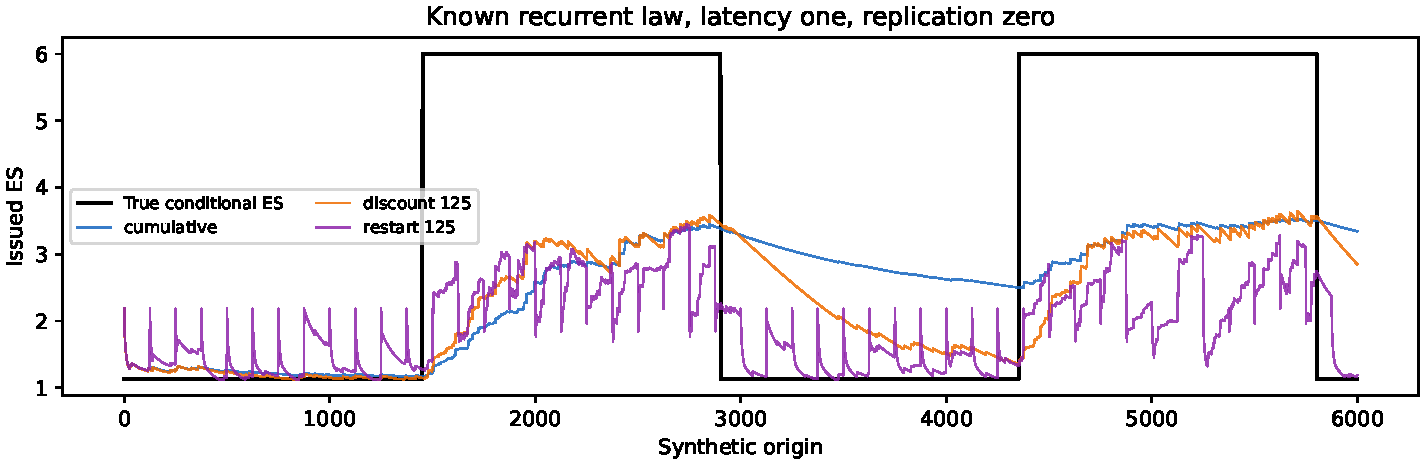
\includegraphics[width=\linewidth]{figures/forgetting_path.pdf}
\caption{Issued ES under the known recurrent law, latency one and replication zero. The black curve is the generating conditional ES, unavailable to all learners. The three displayed learners use $c=0.1$. This synthetic trajectory illustrates retained weights versus periodic resets; inference uses all 32 replications.}\label{fig:forgetpath}
\end{figure}

The old-currency development comparison prevents the synthetic improvement from being promoted automatically. The cumulative rule scores $0.661876$; discounted half-lives 125 and 500 score $0.663055$ and $0.662184$. All six initial interventions are worse on this declared market criterion, so the initial eligibility set is empty. These point differences are development-selection quantities, not statistically certified population disadvantages.

The additional step-scale search exposes the source of a misleading apparent improvement. Discounting at half-life 500 with $c=0.025$ scores $0.655511$ in market development, better than the original cumulative $c=0.1$ rule. However, its changing-law excess is higher than that baseline by $0.30509$ and its worst stationary penalty is $0.32002$. Reducing the step scale improves this historical financial fit while making the controlled learner too slow. Conversely, the $c=0.2$ discounted variants improve changing-law error substantially while worsening the old-market score.

Matched cumulative controls separate those effects. At $c=0.025$, cumulative normalization already scores $0.655652$ on market development; the additional half-life-500 improvement is only $0.000141$. At the same step size, discounting reduces changing-law error by $0.06970$ relative to that slower cumulative rule, yet both remain worse than the original $c=0.1$ comparator on the changing-law criterion. Figure~\ref{fig:forgetmatched} reports the matched comparisons for every discounted and windowed setting. No memory setting in this tested grid simultaneously meets all three eligibility conditions against the original operating rule.

\begin{figure}[htbp]\centering
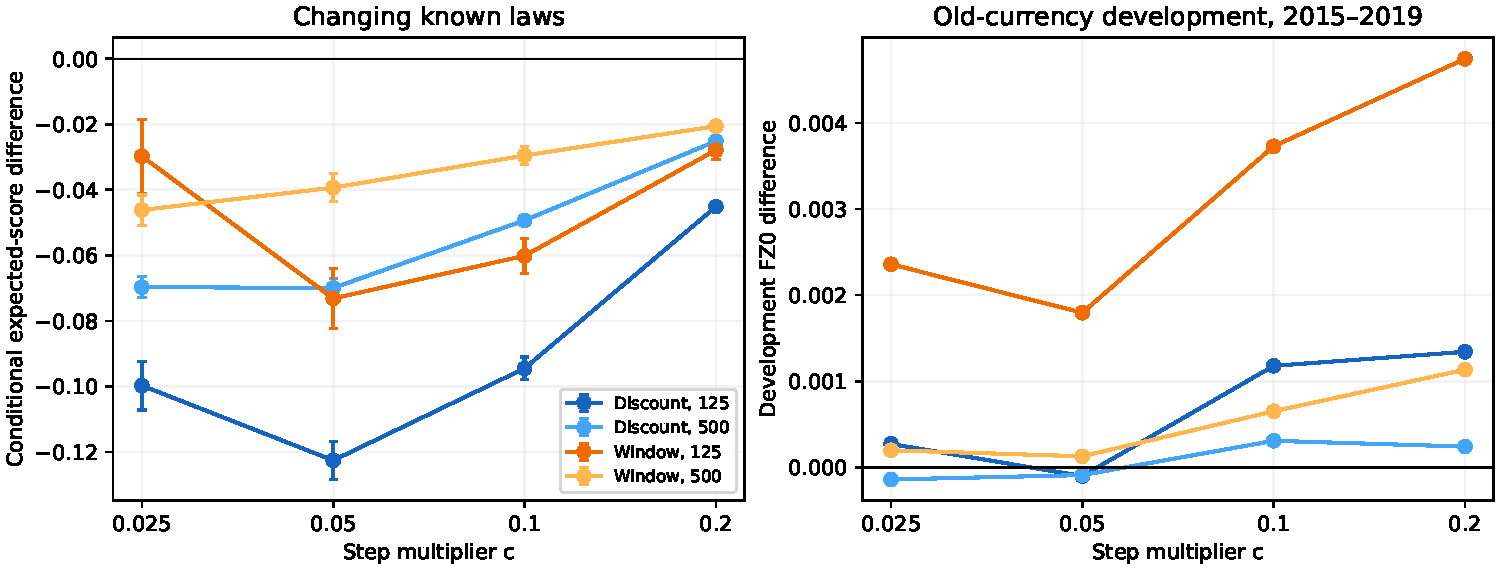
\includegraphics[width=\linewidth]{figures/forgetting_matched_controls.pdf}
\caption{Memory-rule minus cumulative-rule score at the \emph{same} multiplier $c$. Left: conditional expected-score differences on the five changing laws, with marginal paired 95\% Monte Carlo intervals across replication groups. Right: mean FZ0 differences on old-currency development data. All losses and expert banks are paired. These comparisons are diagnostic and do not redefine the original selection criterion.}\label{fig:forgetmatched}
\end{figure}

The final eligible set is empty and the operating rule remains cumulative at $c=0.1$. The transfer gate consequently stops before loading NZD, SGD, KRW or ZAR. No new-currency forecast result, superiority interval or failed market test is asserted for this stage. The finding is instead a measured response benefit under known changing laws and a documented selection tradeoff within this grid. It does not establish an impossibility result for forgetting or for a more contextual combination of learning rates.

\subsection{Independent checks of forgetting and selection}
A lane-first reference implementation uses extended precision and active-set projection, independently of the producer's chronological replay and sorting-based projection. It reconstructs all 224 generated paths, all 9856 synthetic replication--model--latency cases and all 59136 stored scalar score summaries. Uniform-tail expectations are integrated directly over their support; exponential-tail expectations use their analytic survival integral. The largest scalar score discrepancy is $1.83\times10^{-14}$. All 882 retained replication-zero trace arrays agree within the declared absolute/relative tolerances; their largest absolute state discrepancy is $8.91\times10^{-9}$, across arrays that include squared-gradient accumulators. The old-market audit recomputes all 176 development records, with maximum score difference $2.23\times10^{-16}$.

Separate checks cover 16 controller configurations, 32 future-outcome or truncation variants, 48 loss-unit rescalings and 675 fixed-comparator regret inequalities across lanes and reset epochs. The cumulative special case matches the earlier controller. The explicit nonmonotone-step counterexample gives regret $1.0000008$ while the invalid final-step shortcut gives only $0.1000201$; the valid positive-variation bound is $20.1000201$. A separate reduction reconstructs all 370 paired intervals and the empty eligibility set. Its Student critical value is obtained by inverting the incomplete-beta representation of the distribution; the maximum interval discrepancy is $1.12\times10^{-16}$.

These are executed algebraic and independent numerical checks, without directed-rounding certification. They verify the implementation, score integration and declared selection procedure. They do not turn development reuse, constructed laws or the unexecuted transfer plan into independent empirical validation.

\subsection{Component-preserving operational integration}\label{sec:runtimeresults}
The shared runtime passes 56 complete outcome/query-order paths across two- and three-query parity catalogues. The 220 finite-state comparisons also include indistinguishable targets and contradictory evidence. Hosted candidate masks, native result objects, evidence counts, minimax queries and worst-case costs agree exactly with direct component execution. Independent set filtering checks the candidate sets separately. Empty compatibility is reported as conflict.

The maturity study checks 175 combinations of event, receipt and module-operation cutoffs and 187 direct comparisons of snapshots, native snapshot digests and controller states. Separate integer arithmetic reproduces the feedback updates. Delayed completion, receipt order differing from target order, revision replacement, duplicate evidence and the preservation of original forecasts are exercised. Later receipts leave earlier as-of snapshots unchanged. The comparisons preserve the same exact input metadata; different metadata can legitimately change a content identity while retaining the same numerical prediction.

Across 38 invalid-command cases, the exported log and accepted-input budget remain unchanged. Cases include Boolean/integer aliasing, changed identifiers, stale frontiers, altered contracts, backdated owner clocks, future receipt cutoffs and nonfinite arithmetic. Finite positive endpoint pairs producing overflow or underflow in their ratio are rejected without consuming the pending forecast. A late new issue is rejected in the declared-receipt profile; retrospective import succeeds only with its explicit historical basis. Resource tests exercise exact limits and a boundary one byte below the required command size.

Two child processes terminate through \texttt{os.\_exit}: one after preparing SQL changes but before commit, and one after commit before returning its receipt. Recovery and identical retry produce one domain effect in both cases. In the second case the original committed receipt is returned. Separate handles observe current committed state and reject stale command frontiers. Interleaved contracts reproduce their separate executions without changing the other contract's state.

Semantic audit rejects a forged result even after its chain hash is recomputed, and rejects corrupted materialized state. A deliberately reconstructed valid shorter prefix passes unanchored replay, as expected. The separately retained original head/count rejects that same prefix. This distinguishes internal consistency from completeness relative to retained external evidence.

A further preservation study imports 128 already evaluated forecasts for USD, GBP, JPY and CHF at horizons one and five, covering 2--30 January 2026. Eight contracts interleave under one owner and produce 288 accepted commits. All 128 prediction pairs, hit indicators, issue-time states and pre-/post-update controller states agree exactly with the archived numerical execution. Each target remains pending immediately after issue; all eight terminal views agree after reopening and after replaying the saved commands. Initial per-lane controller values are imported from the archive, and update counts restart at the slice boundary; earlier learning is not reconstructed. This explicitly historical import tests execution preservation, not live issuance or vintage availability.

These results establish preservation and fault handling for the supplied bounded reference workloads. Binary64 score equality reuses the existing scoring function; it is not a second mathematical implementation of logarithms or a rounding certificate. No market-selection criterion is reopened, no reserved currency is evaluated, and no increase in forecast accuracy is attributed to the runtime.

\subsection{Generated forecasts, revised learning and modeled proposals}\label{sec:streamresults}
The synthetic stream study generates 136 forecasts, 70 at horizon one and 66 at horizon five. Its eight-expert banks, pooled forecasts, issued weights and severity states match the unchanged batch reference with zero numerical discrepancy in this environment. There are 130 matured targets. Two controlled source corrections preserve the stored issuance objects byte for byte while changing current feedback. Reconstructing both the original and corrected folds supplies 260 independent feedback comparisons. The largest absolute difference is $3.64\times10^{-12}$, occurring in squared-gradient accumulation; the tolerance is $2\times10^{-10}+2\times10^{-11}|x_{\rm ref}|$. An independent simplex projection reproduces the resulting weights.

The six learner lanes, nine fixed comparators and two outcome versions give 108 checks of \eqref{eq:streambound}. Both corrections create nonzero issuance-versus-replay discrepancies. The constructed stale-evaluation example has score excess $138.629436112$, exceeding the invalid residual-free bound $101$. Its signed mismatch is $196.354583211$; the applicable bound is $297.354583211$. The bound is valid but loose in this example. Its value is in preserving the correct comparison, not in establishing improved prediction.

There are 140 exact rational proposal checks, including zero budget, zero quantity cap, equality at a budget boundary and a value just below that boundary. Twenty invalid-input cases leave accepted state unchanged. The model emits no forecasts for 624 warmup deliveries, and retains a separate constant 312-observation history with explicit zero-variance unavailability. The ordinary horizon-one run has 69 targets occurring after issue. The deliberately delayed horizon-five run has 61 targets whose event times are already past at ingestion; all receive the corresponding temporal flag while retaining the same numerical prefix computation. Thus the test exercises the declared distinction rather than inferring future-event lead from source-index order.

The executable demo retains nine issued records through one correction, then emits a tenth forecast from the next received observation. Figure~\ref{fig:streamcorrection} shows the current weight change; no earlier bank, forecast or proposal is rewritten. Fourteen CLI subprocess checks verify explicit profile selection, command retry, inspection, export, anchored audit and rejection of the wrong registry. The previous two-adapter database remains readable with its original profile.

\begin{figure}[htbp]\centering
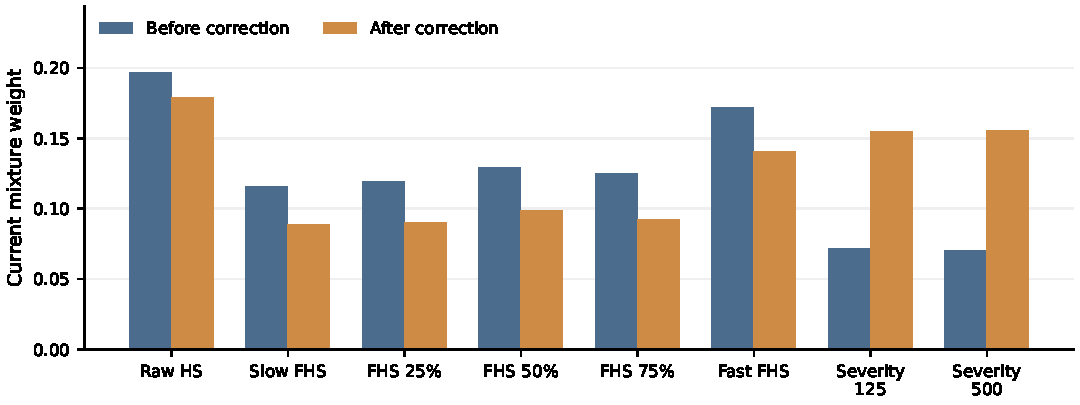
\includegraphics[width=\linewidth]{figures/stream_correction.pdf}
\caption{Current mixture weights before and after a single source correction in the retained synthetic stream demo. The raw value at observation index 316 is multiplied by $33/32$. The correction changes the replayed learning state while preserving all nine previously issued records. These bars show an internal-state response, not forecast-performance improvement.}\label{fig:streamcorrection}
\end{figure}

The historical integration study uses 1384 distinct currency/index observations, delivered 2752 times to eight horizon-specific contracts. It generates 256 forecasts and proposals directly from raw observations, with 232 matured targets and 24 pending targets. The first source observation is 4 January 1999 and the latest used endpoint is 5 May 2000. All 16472 compared numerical scalars---expert outputs, issued weights, severity states, gradients and update states---are byte-identical to the unchanged batch reference in the executed environment; the declared absolute/relative tolerance is $2\times10^{-13}$/$2\times10^{-12}$. All 256 proposal boundaries satisfy the exact rational checks, and all eight final views survive semantic reopening. The shared owner records 2760 unique commits, including eight bindings.

These checks establish a complete bounded execution path from received observations to predictions, read-only proposals and corrected learning. The historical study measures implementation agreement under its explicit initialization and synthetic receipt convention. It supplies neither another market-accuracy result nor evidence that the existing superiority criterion has been met.

\subsection{Preserved outputs and reduced execution work}\label{sec:incrementalresults}
The independent incremental verifier passes 1058 direct state-and-result comparisons and 1083 view comparisons, all in exact canonical bytes. It also compares 325 owner transition results and verifies a 326-commit store after cold reopening. The tests include 718 warm-cache gradient-work bounds, 47 endpoint-locality checks and 23 malformed-input, arithmetic, historical-domain or capacity rejections. Forks, rewinds, same-value revisions, cache clearing, returned-object mutation and a failure after speculative computation preserve reference behavior. Seven direct-state mutations test actual-field dependency keys without treating a supplied digest as authority. These diagnostic states are distinguished from accepted owner histories. Twenty CLI subprocess checks retain the original stream demo and compare its issued forecasts and snapshots with incremental execution.

The historical-domain tests reveal why locality of output computation is insufficient for acceptance equivalence. Accepted corrections at source indexes 80--85 create a nonfinite five-interval return outside the current 250-scenario window while adjacent returns remain finite. Both implementations reject the next forecast, then recover after repair. The optimized evaluator preserves the reference's historical validity checks rather than accepting a current row in isolation.

The efficiency study adds 1600 sequential transition comparisons, 90 paired terminal branches and six paired durable-owner trials. All compared canonical-output digests agree. Table~\ref{tab:incrementalwork} reports the complete 800-observation runs. At horizon one, each of the 489 mature contributions is evaluated once by incremental execution, compared with 119805 evaluations in full replay. The horizon-five counts are 481 and 115921. The 490 and 486 eligible forecast origins produce six current scenario rows each, rather than all rows through every origin.

\begin{table}[htbp]
\centering\small
\caption{Work and elapsed time over the two synthetic 800-observation trajectories. Reference counts follow the executed full-replay loop bounds; incremental counts are recorded by the evaluator. One variance row updates both decay components, and one scenario row contains 250 values. Complete-path times are single descriptive executions, not repeated timing estimates.}\label{tab:incrementalwork}
\begin{tabular}{@{}lrrrr@{}}
\toprule
 & \multicolumn{2}{c}{$h=1$} & \multicolumn{2}{c}{$h=5$}\\
\cmidrule(lr){2-3}\cmidrule(l){4-5}
Quantity & Reference & Incremental & Reference & Incremental\\
\midrule
Gradient evaluations & 119805 & 489 & 115921 & 481\\
Scenario rows & 721770 & 2940 & 710046 & 2916\\
Variance rows & 485590 & 740 & 483570 & 740\\
Numerical-call time (s) & 18.627 & 8.621 & 17.606 & 8.529\\
Complete adapter time (s) & 36.774 & 27.124 & 37.104 & 26.657\\
\bottomrule
\end{tabular}
\end{table}

The complete-trajectory execution is approximately 26.2\% and 28.2\% shorter. This is much smaller than the reduction in repeated gradient or scenario-row evaluation, because full-prefix array operations, dependency checking and canonical materialization remain. Figure~\ref{fig:incrementalexecution} distinguishes numerical-call time from the complete adapter transition.

\begin{figure}[htbp]
\centering
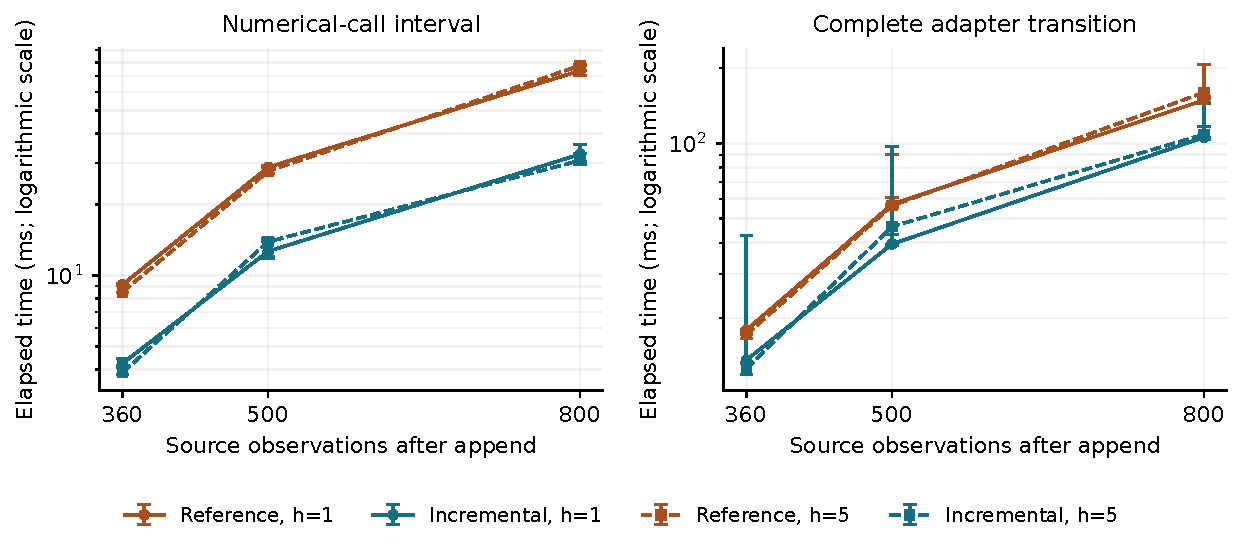
\includegraphics[width=\linewidth]{figures/incremental_execution.pdf}
\caption{Synthetic append timings at three target prefix lengths. Points show medians of three local trials and bars their observed minimum--maximum ranges. The numerical-call interval includes its own object construction; the complete adapter additionally validates and materializes the whole transition. These measurements exclude the SQLite owner, which is measured separately. Lines connect measured cases only.}\label{fig:incrementalexecution}
\end{figure}

For an append completing 800 observations, median complete-adapter latency is 148.895 versus 105.681\,ms at $h=1$, and 159.864 versus 108.564\,ms at $h=5$. The corresponding medians of paired reference/incremental ratios are 1.373 and 1.447; these need not equal ratios of the separately computed medians. The numerical-call ratios are 2.259 and 2.292. Across all 30 terminal case groups, median paired complete-adapter ratios range from 1.037 to 1.495. Individual repeated ratios range from 0.407 to 2.279, so the observations do not establish a uniform timing advantage on every invocation.

Corrections followed by an append include deferred variance work. At 800 observations, the median paired complete-adapter ratios for early and recent correction bundles are 1.361 and 1.382 for $h=1$, and 1.225 and 1.080 for $h=5$. These are two-operation bundles, not per-command latency estimates. The old correction can require a long variance suffix and many subsequent projections even when only two gradients change.

The singleton-registry owner experiment completes a 360-observation history. Its median durable append times are 39.743 versus 33.104\,ms for $h=1$, and 37.227 versus 30.559\,ms for $h=5$. Fresh cold semantic reopening takes 2.254 versus 2.070\,s and 2.066 versus 1.997\,s, respectively. The smaller audit gains are consistent with retained command replay and complete-history verification. All timings use the recorded Linux environment with Python 3.12.14, NumPy 2.3.5 and SciPy 1.17.0; three repeats do not establish portable throughput or a statistical confidence interval. The measured improvement is computational under the fixed contract. Forecast quality and the signed replay-mismatch bound are unchanged.

\subsection{Equivalent durable-owner execution}\label{sec:fastownerresults}
The independent owner verification passes 1344 direct canonical receipt comparisons and 1346 comparisons of every field in all SQL tables. The five paths cover the original two-adapter profile and the reference and incremental generated-stream profiles at horizons one and five. The copy checks include 261 valid values and 18 invalid cases, all 128 ASCII code points, exact integer limits, depth 64 acceptance and depth 65 rejection, recursive dictionary order and expansion of mutable aliases. Fourteen invalid-reducer rejections across the two owners preserve committed rows. Both owners reject the exercised noncanonical, duplicate-key and floating-point stored states before using them.

Cross-owner reopening and full audits agree. A concurrent comparison admits exactly one command against the same prior head. Actual process termination before commit leaves no new event; termination after commit retains the event and its exact retry receipt. These tests exercise process failure, not physical power removal. The identity-sensitive counterexample produces different results as expected outside the value-based adapter contract, and is retained explicitly.

The separate CLI study passes 103 subprocess commands. Original default demonstration bundles remain equal for all three profiles; twelve creator/opener combinations preserve exact journals and anchors. The preceding 20-command incremental CLI regression also passes with the changed entry point. All twelve previously retained core and research source files remain byte-identical; owner selection does not alter adapter fingerprints. These comparisons concern the stored data contract and numerical outputs, not equality of Python allocation identities.

The matched timing experiment independently compares 4133 canonical receipts, 160 stored state/meta representations, 7543 complete journal rows and five actual API exports without a mismatch. These counts exclude the separate 33-command warmup. Source hashes remain unchanged throughout the run. On the integer-register workload, the median of seven trial-average command times changes from 0.322 to 0.245\,ms for 32 registers, from 0.688 to 0.432\,ms for 256, and from 3.461 to 1.794\,ms for 2048. The respective median paired reference/fast ratios are 1.343, 1.605 and 1.915. Each trial average includes 100 individually committed commands; its inverse does not include command construction or verification and is not sustained end-to-end throughput.

\begin{table}[H]
\centering\small
\caption{Durable stream execution near 800 observations. Each row summarizes seven successive, correlated paired trials. Latency columns are separate medians in milliseconds; the ratio column is the median of paired reference/fast ratios and need not equal their quotient. Append trials start at 800--818 observations; early and recent correction bundles start at 801--819 and 802--820, respectively. Each correction bundle includes its following append.}\label{tab:fastowner}
\begin{tabular}{rlrrr}
\toprule
$h$ & Operation & Reference (ms) & Fast (ms) & Paired ratio\\
\midrule
1 & Append & 263.009 & 180.304 & 1.413\\
1 & Early correction + append & 552.569 & 387.051 & 1.368\\
1 & Recent correction + append & 548.412 & 376.928 & 1.409\\
5 & Append & 280.570 & 203.852 & 1.458\\
5 & Early correction + append & 568.422 & 413.757 & 1.421\\
5 & Recent correction + append & 584.864 & 408.533 & 1.484\\
\bottomrule
\end{tabular}
\end{table}

Across all 18 transition groups at the three history neighborhoods, median paired ratios range from 1.337 to 1.499. Individual transition pairs range from 1.117 to 1.991. Full-view group medians also improve, although one of the 42 individual view pairs is slower, with a ratio of 0.873. The complete evolving path contains 821 source appends and 42 corrections. Summing the 863 unprofiled submit calls gives 80.207 versus 56.393\,s for $h=1$ and 79.207 versus 55.700\,s for $h=5$: reductions of 29.69\% and 29.68\%. These single-path sums exclude binding, views, audits, reopening, input construction and exactness checks. They compare two owners using the same already-incremental numerical adapter, not two forecast models.

\begin{figure}[H]
\centering
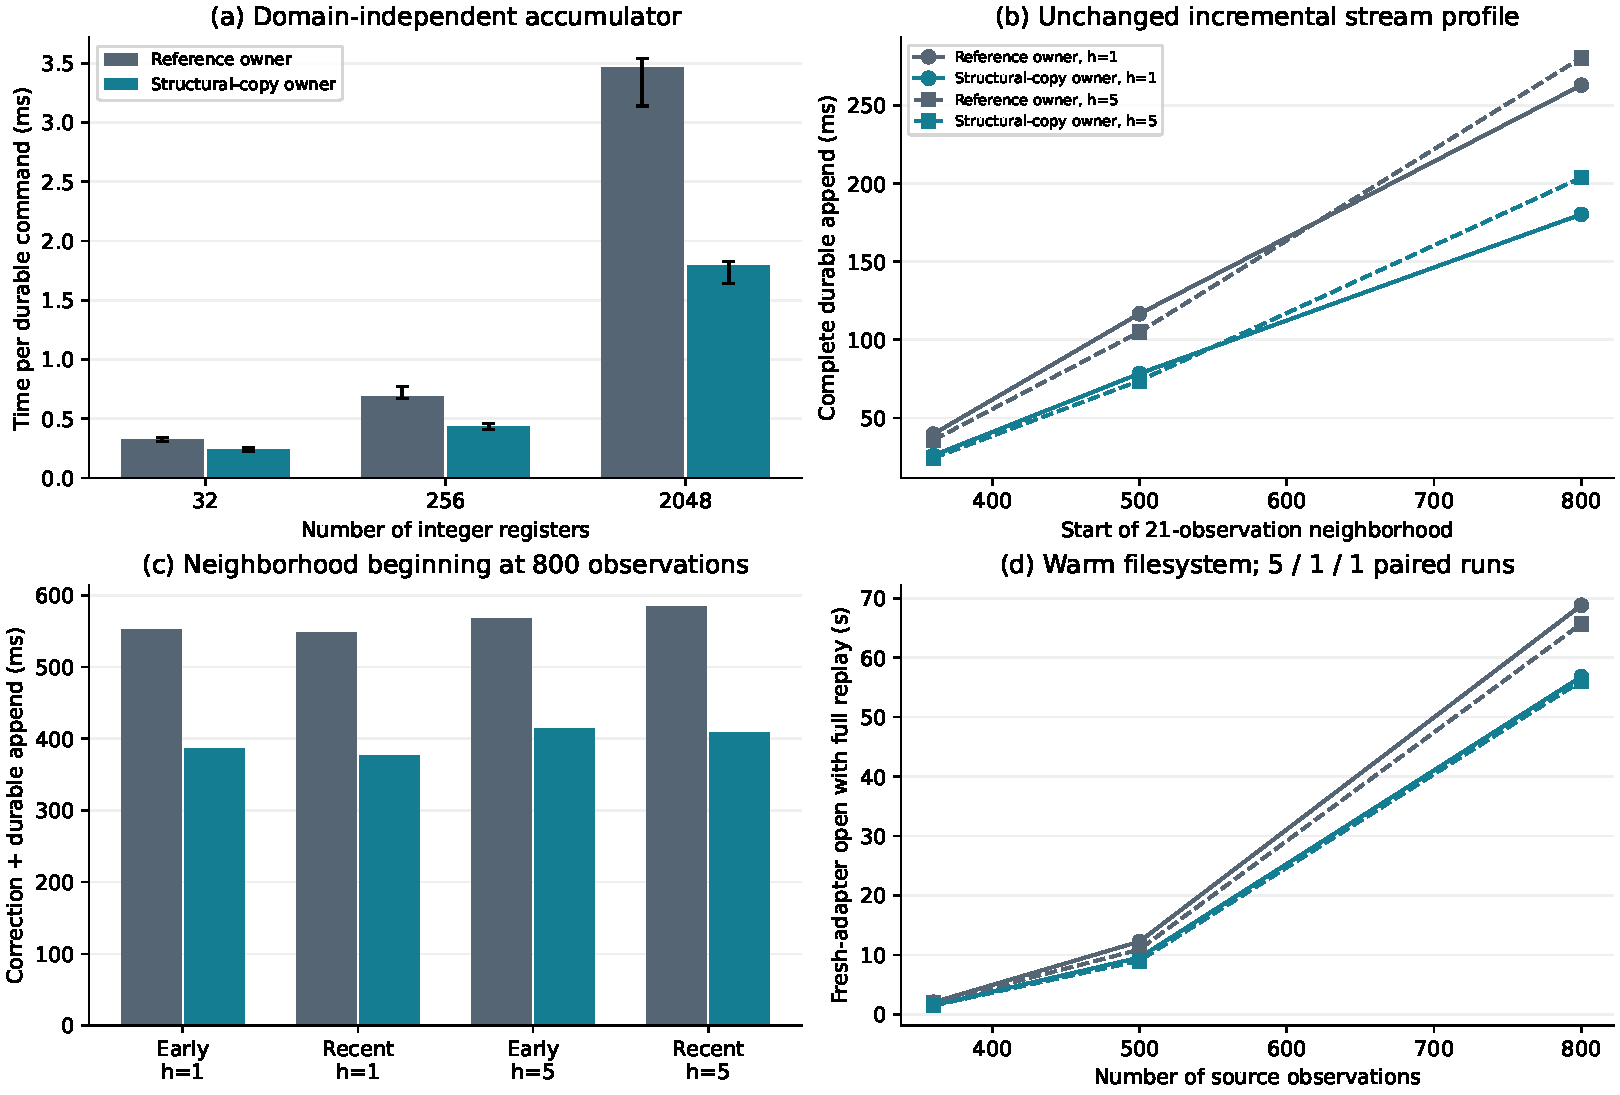
\includegraphics[width=\textwidth]{figures/fast_owner_execution.pdf}
\caption{Measured owner execution under an unchanged numerical adapter. Panel (a) shows medians of seven trial averages with their observed minima and maxima, not confidence intervals. Panel (b) shows separate medians of seven successive neighborhood append trials; panel (c) shows both early- and recent-correction bundles near 800 observations. Panel (d) uses five paired fresh-adapter openings at 360 observations and one descriptive pair at each larger checkpoint; the filesystem cache is not flushed. Colors identify owners; markers and line styles in (b,d) identify owners and horizons as in the legend.}\label{fig:fastowner}
\end{figure}

Complete semantic reopening remains costly. At 800 observations, a fresh owner and numerical adapter take 68.812 versus 56.808\,s for $h=1$ and 65.695 versus 56.082\,s for $h=5$. These are individual pairs with a warm filesystem, not cold-device latency estimates. Retaining complete state and result histories also preserves the journal's storage growth. The refinement reduces repeated representation work; it does not bound replay or storage cost as history grows.

A separate profiled final append records seven calls to the original JSON round-trip copy in the reference owner and one in the alternative, together with six checked structural copies. Strict JSON parse calls decrease from 17 to 11 for either horizon. Canonical serialization calls decrease from 560 to 546 for $h=1$ and from 552 to 538 for $h=5$. The adapter and audit still perform their own serialization work. Profiled timings are excluded from all efficiency summaries; recursive validation counts do not represent total arithmetic or validation cost.

The environment is Linux on an AMD EPYC 9V74 host, Python 3.12.14, NumPy 2.3.5 and SQLite 3.53.1, with OpenMP, OpenBLAS and MKL thread variables set to one. Alternating pair order limits a simple order bias but does not remove shared-machine variation. Seven evolving trials give descriptive local comparisons, not independent statistical replicates or portable service guarantees. These ratios must not be multiplied by the preceding adapter experiment's ratios, which use a different seed and measurement protocol.

\subsection{Complete replay with expected-byte verification}\label{sec:replayresults}
The expected-byte owner passes the exercised reference comparisons: 1,344 profile receipt comparisons, 1,346 complete database-content comparisons, fourteen invalid-reducer rejections across the reference and expected-byte owners, and the concurrent two-connection admission check. All 53 added corrupted database cases are rejected by the reference, structural-copy and expected-byte owners. The nested-state boundary accepts depths 0, 60 and 61 and rejects 62 and 63 for all three owners under the specific fixture convention. The counting adapter records four applications on opening and eight after a subsequent audit in every accepted case. Another 103 actual CLI commands check all three registry profiles, retained demonstrations, cross-owner continuation and rejection behavior.

\begin{table}[H]\centering\small
\caption{Complete fresh-owner replay on synthetic histories. Fast and replay columns give median opening seconds; the ratio is the median of paired fast/replay times, with its observed range. Register size denotes width; stream size denotes observations. Database preparation and output comparisons are excluded.}\label{tab:replayopens}
\begin{tabular}{llrrrr}\toprule
Case & Size & Fast (s) & Replay (s) & Ratio & Range \\ \midrule
$h=1$ & 360 & 1.922 & 1.593 & 1.204 & 1.189--1.206 \\
$h=1$ & 500 & 10.415 & 8.002 & 1.302 & 1.266--1.317 \\
$h=1$ & 800 & 61.164 & 45.860 & 1.339 & 1.334--1.374 \\
$h=5$ & 360 & 1.872 & 1.577 & 1.187 & 1.184--1.194 \\
$h=5$ & 500 & 10.057 & 7.753 & 1.297 & 1.286--1.331 \\
$h=5$ & 800 & 63.341 & 46.597 & 1.338 & 1.276--1.408 \\
Registers & 32 & 0.162 & 0.086 & 1.862 & 1.793--2.094 \\
Registers & 256 & 0.307 & 0.185 & 1.633 & 1.366--1.701 \\
Registers & 2048 & 1.376 & 0.989 & 1.394 & 1.343--1.516 \\
\bottomrule\end{tabular}\end{table}
For horizon $h=1$ at 800 observations, the median opening time falls from 61.16 to 45.86 seconds (25.0\%); the unchanged database occupies 303.10 MB (decimal).
For horizon $h=5$ at 800 observations, the median opening time falls from 63.34 to 46.60 seconds (26.4\%); the unchanged database occupies 293.63 MB (decimal).


These measurements use fresh adapters and full journal replay; they are not checkpoint-loading times. The implementation preserves the database and terminal outputs, while avoiding repeated parsing of stored derived values. The histories still retain complete forecast outputs and state, and opening cost grows substantially with history length. The audit override preserves the forecast outputs and storage format and inherits the live submission implementation unchanged.

\subsection{Bounded native signatures and inherited engine limits}\label{sec:nativepseresults}
The packed-orbit tests exhaust all 1099 labelled simple graphs with one through five vertices and check 48 seeded six- and seven-vertex graphs against an independent indexed-matrix action. Nine complete signatures agree with the unchanged dense implementation in exact canonical bytes. Invalid inputs are rejected, and the inherited cross-size padded-hash collision is reproduced explicitly.

The focused current-environment comparison produces identical 1257237-byte serializations of 32 selected state snapshots and the complete returned crystals. Hidden fields such as internal memory indexes, pending candidates and navigator state are outside that snapshot format. The existing harness's serialized comparison outputs also agree between the current reference and optimized build; those outputs include state digests rather than all underlying state bytes.

\begin{table}[H]
\centering\small
\caption{Focused synthetic native commit workloads. Throughput ratios are medians of three paired ratios; brackets show their observed range. Each pair compares medians of five fresh-engine runs. Allocation counts are per observation from separate untimed executions. The eight-source row does not enter the optimized signature path.}\label{tab:packednative}
\begin{tabular}{rrrr}
\toprule
Sources & Paired speed ratio [range] & Reference allocations & Packed allocations\\
\midrule
3 & 3094.55 [2710.85, 3445.32] & 90605.13 & 163.46\\
5 & 1222.68 [1031.68, 1285.01] & 54474.55 & 187.35\\
7 & 513.37 [500.39, 536.59] & 39624.25 & 157.82\\
8 & 1.022 [0.933, 1.025] & 131.14 & 131.14\\
\bottomrule
\end{tabular}
\end{table}

Table~\ref{tab:packednative} identifies a severe avoidable cost in the eligible signature branch. For three sources, the median of the per-run median tick latencies changes from 356.199 ms to 0.101 ms; the corresponding values are 357.751 to 0.285 ms for five and 357.819 to 0.662 ms for seven. These latency summaries and paired throughput ratios are distinct statistics. The eight-source control remains near its original cost, as do the existing harness's workload groups, whose paired median ratios range from 0.988 to 1.063. The large focused gains therefore do not describe ordinary ingestion, arbitrary graph sizes, the entire Gabriel runtime or prediction quality.

The supplied historical fixture does not match unchanged upstream execution in the current environment: 23 of 78 state digests and one crystal digest differ. Its originating stored state values are unavailable for diagnosing the cause, which remains unresolved. The unfiltered upstream test command consequently fails. With this single test explicitly filtered, 433 reference tests and 438 alternative tests pass; one documentation test is ignored in each build. The historical fixture is preserved. These facts preclude treating the current checks as demonstrated portability of all historical bytes.

Independent inherited-code counterexamples also report a partial-Lanczos spectral gap of zero on a specified 32-vertex complete graph whose symmetrized Laplacian gap is 16, and four clusters under a declared maximum of two. Other source findings include time-dependent multiscale branches and incomplete evidence-field binding. They remain separate from the bounded signature refinement. In particular, equal signature outputs cannot prove complete-engine equivalence for arbitrary execution schedules when other branches read elapsed time. The optional native component supplies a verified finite optimization and a reproducible analysis boundary, not an authority to certify its surrounding heuristic model.

\subsection{Exhaustively verified finite orbit data}\label{sec:indexresults}
The independent checker accepts all 2,097,152 graph witnesses and all 12,582,912 adjacent-transposition closure checks. It recomputes the 1,044 class minima and cardinalities and verifies the associated stabilizer orders. The fourteen invalid certificates are rejected; replacing the empty graph's witness by the reversed vertex permutation is correctly accepted. Two generator runs reproduce the three delivered binary files byte for byte. Source hashes, compiler identification, actual commands and checker outputs are retained with the certificate.

This executed result establishes a complete finite lookup representation of the specified orbit data. The following integration experiment evaluates its native consumer separately; the offline certificate alone supplies neither floating-point equivalence nor an engine speed ratio.

\subsection{Integrated lookup and exact-input signature reuse}\label{sec:indexedintegration}
The indexed evaluator matches the packed evaluator's complete canonical signatures for all 1,099 labelled graphs through five vertices and 128 seeded graphs at six and seven vertices. Cache tests compare complete serialization and every floating-point field's raw bits on 448 sampled inputs and immediate repeats. The additional tests cover validation ordering, all matrix positions of signed zero, dimension and labelled-input identity, collisions, caller mutation, separate threads, reset and 1,024 distinct inputs beyond capacity. The executed workspace run passes 449 tests with one documentation test ignored and the preserved historical fixture explicitly filtered. The unfiltered run reaches and fails that fixture; its earlier discrepancy remains unresolved.

The three engine goldens are byte-identical over 1,257,369 bytes each; the complete-signature goldens are identical over 3,173,601 bytes each. These are exact comparisons of the stated outputs on the stated traces, not a proof about every private engine field or every timing-dependent execution. An archived measured-source snapshot retains the recorded hashes, and the compiled table inputs retain the independently certified bytes. The performance experiment executes 16,000 timed engine ticks, 80 separate first macrosteps and 114,688 timed complete-signature calls.

\begin{table}[H]\centering\small
\caption{Complete native engine comparisons. Entries are median paired ratios with observed ranges across five pairs. Ratios above one favour indexed and memoized execution, respectively. Warm rows use observation throughput; first-call rows use inverse elapsed time for the first macrostep in a fresh process.}
\label{tab:indexedengine}
\begin{tabular}{llrr}\toprule
Interval & Sources & Indexed / packed & Memoized / indexed \\\midrule
Warm & 3 & $1.662\,[1.577,\,1.750]$ & $1.243\,[1.208,\,1.290]$ \\
Warm & 5 & $1.320\,[1.234,\,1.400]$ & $1.075\,[1.057,\,1.187]$ \\
Warm & 7 & $1.177\,[1.124,\,1.278]$ & $1.014\,[0.987,\,1.114]$ \\
Warm & 8 & $0.989\,[0.925,\,1.042]$ & $0.985\,[0.975,\,1.084]$ \\
\midrule
First call & 3 & $14.154\,[8.891,\,15.838]$ & $0.851\,[0.776,\,0.911]$ \\
First call & 5 & $5.896\,[5.615,\,7.865]$ & $0.920\,[0.760,\,1.007]$ \\
First call & 7 & $4.008\,[3.229,\,4.854]$ & $0.937\,[0.773,\,1.397]$ \\
First call & 8 & $0.983\,[0.748,\,1.411]$ & $1.066\,[0.879,\,1.931]$ \\
\bottomrule\end{tabular}
\end{table}

\begin{table}[H]\centering\small
\caption{Complete-signature kernel comparisons in one executable. Entries are median paired ratios with observed ranges across seven pairs of 512 calls. Hit rates cover timed memoized calls only, after warmup. Each changing corpus is reused across passes.}
\label{tab:indexedmicro}
\begin{tabular}{llrrr}\toprule
$n$ & Inputs & Indexed / packed & Memoized / indexed & Hits (\%) \\\midrule
3 & Fixed & $5.053\,[3.048,\,5.797]$ & $97.347\,[90.132,\,100.662]$ & 100.00 \\
3 & Changing & $4.872\,[4.624,\,7.482]$ & $77.235\,[53.230,\,104.206]$ & 100.00 \\
5 & Fixed & $7.202\,[6.375,\,7.767]$ & $66.855\,[39.187,\,70.227]$ & 100.00 \\
5 & Changing & $4.690\,[4.028,\,5.135]$ & $1.335\,[1.280,\,1.510]$ & 33.59 \\
5 & Collision & $4.708\,[4.415,\,5.488]$ & $0.978\,[0.754,\,1.094]$ & 0.00 \\
7 & Fixed & $9.865\,[8.395,\,10.451]$ & $38.120\,[34.150,\,141.727]$ & 100.00 \\
7 & Changing & $3.167\,[2.803,\,3.282]$ & $1.034\,[0.756,\,1.323]$ & 14.45 \\
7 & Collision & $3.875\,[3.280,\,4.236]$ & $0.970\,[0.880,\,1.232]$ & 0.00 \\
\bottomrule\end{tabular}
\end{table}


Table~\ref{tab:indexedengine} shows warm complete-engine throughput ratios of 1.662, 1.320 and 1.177 for indexed versus packed evaluation at three, five and seven sources. Thus eliminating the remaining permutation scan improves the complete tested path, although substantially less than the isolated kernel. The eight-source control has ratio 0.989 and executes no bounded signature. First-call ratios of 14.154, 5.896 and 4.008 include avoiding the packed evaluator's lazy permutation preparation; they exclude process startup and do not measure a cold filesystem.

Exact-input reuse adds warm complete-engine ratios of 1.243, 1.075 and 1.014 against the indexed implementation. At seven sources its observed pair range crosses one. The corresponding fixed-graph kernel ratios are 97.347, 66.855 and 38.120, because a hit avoids the complete remaining signature calculation. The signature occupies only part of a macrostep, so those kernel ratios do not describe the whole engine. No product of these ratios with the earlier dense-to-packed measurements is reported.

The changing-input experiment exposes the importance of reuse. Its timed hit rates are 100\%, 33.594\% and 14.453\% at three, five and seven vertices. All eight three-vertex inputs fit without collisions after warmup; the seven-vertex corpus is unique within a pass but repeats across passes. The memoized kernel ratios fall to 1.335 at five vertices and 1.034 at seven. Alternating colliding inputs produces zero hits and median ratios 0.978 and 0.970, with the observed ranges crossing one. It therefore supplies no measured acceleration and has slightly higher median cost in these runs. The first engine call likewise favours uncached indexed evaluation in all three eligible median comparisons, reflecting initialization and miss work rather than a warm hit.

Packed evaluation remains the default; indexed and memoized execution are explicit build choices. The index provides the clearer measured improvement across these eligible workloads. Memoization is a conditional addition for repeated labelled graphs, with a per-thread entry bound and an exact output contract. Neither refinement changes the Python owner, financial forecasts or inherited PSE model assumptions. A changing/sparse whole-engine workload and memory-use measurements are outside this experiment; the changing and collision controls evaluate the complete signature function only.


\subsection{Guarded spectral reuse on sparse and growing graphs}\label{sec:spectralphaseresults}
The executed all-feature workspace run passes 461 tests, with one documentation test ignored and exactly the preserved historical fixture filtered. The unfiltered final-source run still fails that fixture. The CTQW checks compare every returned binary64 field in 1,500 parameter cases, including threshold-adjacent inputs, ragged spectra, signed zeros and exceptional-input fallback. Four malformed-rank cases compare failure behavior. Separate guard-boundary tests exercise admission and delegation. An independent original-body oracle checks the topology refactor and retained eigensystem on 21 graph/rank combinations. Core differential checks exercise sparse commits, errors and rejections, plus the 100/101, 199/200/201 and 500/501 size boundaries. These checks preserve the stated computation; they do not certify the inherited spectral model.

All four builds produce identical 19,658,993-byte golden outputs over the 233 public-input steps. The scope is complete serialized crystals and the declared selected-state fields, not every private engine field or every underlying NaN payload. The measured study contains 30 timed processes and 3,600 fresh-engine episodes, comprising 43,560 committed macrosteps. Each measured eligible repeated path gives only cache hits; each measured eligible acquisition episode gives only misses after its explicit reset. No measured signature calls occur at eight or sixteen vertices.

\begin{table}[H]\centering\small
\caption{Repeated sparse path: complete native macrostep throughput. Entries are median paired candidate/reference ratios with observed minimum and maximum over five alternating process pairs. Each process contains 12 fresh-engine episodes per case. Indexed time is the median of the five per-process median times in the first comparison; it is descriptive, not the denominator of every ratio.}
\label{tab:phaserepeatedpath}
\resizebox{\textwidth}{!}{\begin{tabular}{rrrrr}\toprule
$n$ & Indexed ($\mu$s/tick) & Hoisted / indexed & Shared / hoisted & Memoized / shared \\\midrule
3 & 56.221 & $1.216\,[1.134,\,1.270]$ & $1.026\,[0.941,\,1.072]$ & $1.527\,[1.372,\,1.580]$ \\
5 & 229.612 & $1.916\,[0.951,\,2.074]$ & $1.054\,[1.030,\,1.157]$ & $1.110\,[1.077,\,1.259]$ \\
7 & 554.525 & $2.837\,[1.372,\,3.185]$ & $1.106\,[0.954,\,1.110]$ & $1.041\,[1.016,\,1.226]$ \\
8 & 754.430 & $3.605\,[2.406,\,4.529]$ & $1.072\,[0.989,\,1.090]$ & $0.998\,[0.938,\,1.068]$ \\
16 & 5651.285 & $5.871\,[3.585,\,6.004]$ & $1.050\,[0.991,\,1.157]$ & $1.018\,[0.941,\,1.055]$ \\
\bottomrule\end{tabular}}
\end{table}

\begin{table}[H]\centering\small
\caption{Cold edge acquisition: complete native macrostep throughput. Entries are median paired candidate/reference ratios with observed minimum and maximum over five alternating process pairs. Each process contains 12 fresh-engine episodes per case. Indexed time is the median of the five per-process median times in the first comparison; it is descriptive, not the denominator of every ratio.}
\label{tab:phasecoldacquisition}
\resizebox{\textwidth}{!}{\begin{tabular}{rrrrr}\toprule
$n$ & Indexed ($\mu$s/tick) & Hoisted / indexed & Shared / hoisted & Memoized / shared \\\midrule
3 & 57.396 & $1.307\,[1.142,\,1.335]$ & $1.046\,[0.996,\,1.053]$ & $1.009\,[1.003,\,1.169]$ \\
5 & 235.223 & $1.970\,[1.214,\,2.121]$ & $1.098\,[1.039,\,1.162]$ & $0.987\,[0.878,\,1.099]$ \\
7 & 549.971 & $2.571\,[1.387,\,2.747]$ & $1.020\,[0.977,\,1.038]$ & $1.007\,[0.924,\,1.027]$ \\
8 & 696.234 & $3.422\,[2.001,\,3.535]$ & $1.033\,[0.982,\,1.058]$ & $1.034\,[0.967,\,1.116]$ \\
16 & 4311.169 & $4.840\,[2.965,\,4.955]$ & $1.055\,[1.019,\,1.084]$ & $1.016\,[0.994,\,1.035]$ \\
\bottomrule\end{tabular}}
\end{table}


Phase reuse is the principal measured improvement. Its median full-engine throughput ratios range from 1.216 to 5.871 across the ten cases. At sixteen vertices the repeated-path ratio is 5.871, with an observed pair range of 3.585--6.004; acquisition gives 4.840, with range 2.965--4.955. At eight vertices the medians are 3.605 and 3.422. These sizes execute no bounded graph signature during the measured interval, establishing a benefit on a different engine path from finite orbit lookup. The five-vertex repeated-path range includes one, so the positive median is not an improvement in every individual pair. Broad timing ranges remain visible rather than being replaced by a single best run.

Sharing the already constructed eigensystem adds median ratios of 1.020--1.106 over the phase-reuse build. Several pair ranges include one. The source-level removal of a decomposition is exact, but these small-workload measurements support a substantially smaller and less uniform elapsed-time gain than phase reuse. Larger graphs without CTQW were functionally checked at the size boundaries, not timed in this experiment.

Memoization adds repeated-path ratios of 1.527, 1.110 and 1.041 at three, five and seven vertices. Under cleared-cache acquisition the corresponding medians are 1.009, 0.987 and 1.007: retaining completed signatures supplies no clear practical gain on these all-miss intervals. The ineligible eight- and sixteen-vertex cache controls also fluctuate around one, showing the scale of process/build variation when this mechanism performs no measured calls. The results favor phase reuse as the broader tested change and retain cache selection as a workload-dependent choice.

These are full native macrostep measurements under the controlled extraction and morphology configuration in Section~\ref{sec:spectralphaseprotocol}. They are not default-workload, durable-owner, financial-prediction or system-wide performance estimates. No ratio is multiplied by the historical signature factors or by a separately measured refinement. Packed signatures and the reference spectral path remain the default; the documented build features select the alternatives explicitly. Memory consumption, concurrency scaling, graphs above sixteen vertices and external traffic remain outside the timing study.

\subsection{Conditioned queries with exact structural dispatch}\label{sec:conditionedresults}
The optional state-query API passes fifteen Rust tests, including independent
matrix-power references, complex unnormalized states, degeneracy, inverse
propagation, zero-time bit preservation, malformed inputs and overflow. Five
geometric tests check the twelve distinct dihedral permutations,
all 144 ordered products, inverse and generator relations, and both reflection
axis types. The complete all-feature native run passes 481 tests, with one
documentation test ignored and the same named historical fixture explicitly
filtered. A separate run of that fixture still fails; no expected output was
changed to force agreement. The existing topology source differs only by the
documented module export, and all ten Python runtime sources remain unchanged.

Seven fresh measurement processes complete all eleven cases and 385 paired
batches for each of setup, preparation and queries. The query phase executes
2,401,280 state queries per backend, or 4,802,560 in total. Table~\ref{tab:conditionedwalk}
reports the separate ratios. On the $w=0.25$ cliques, median query speed ratios
increase from 3.421 at seven vertices to 63.879 at 128 vertices. Observed process
median ranges are $[3.219,3.660]$ and $[59.198,68.420]$ respectively. At thirteen
vertices the median ratio is 5.980 for $w=0.25$ and 6.511 for $w=1$. Plan
construction also improves, but its cost and source-preparation cost are not
included in the repeated-query ratios or multiplied into them.
\begin{table}[H]\centering\small
\caption{Conditioned full-state queries. Median Spectral/Auto elapsed-time ratios and observed ranges of seven process medians, each based on five alternating pairs. Setup and source preparation are timed separately. One in sixteen queries is at zero time. These are synthetic API measurements, not whole-engine gains.}
\label{tab:conditionedwalk}
\resizebox{\textwidth}{!}{\begin{tabular}{lrrrr}\toprule
Graph & $n$ & Setup ratio & Prepare ratio & Query ratio [range]\\\midrule
Clique & 7 & 3.70 & 2.05 & $3.42\,[3.22,\,3.66]$ \\
Clique & 13 & 4.15 & 3.20 & $5.98\,[5.49,\,6.31]$ \\
Clique & 32 & 4.78 & 14.93 & $15.91\,[14.48,\,16.88]$ \\
Clique & 64 & 6.05 & 45.18 & $31.17\,[27.84,\,33.45]$ \\
Clique & 128 & 10.32 & 100.55 & $63.88\,[59.20,\,68.42]$ \\
Clique ($w=1$) & 13 & 4.02 & 3.23 & $6.51\,[6.04,\,7.75]$ \\
Clique (guard) & 13 & 0.96 & 1.00 & $1.03\,[0.96,\,1.11]$ \\
Near-clique & 13 & 1.00 & 1.00 & $1.02\,[0.91,\,1.07]$ \\
Near-clique & 64 & 1.00 & 1.00 & $1.01\,[0.96,\,1.04]$ \\
Path & 13 & 0.99 & 0.98 & $1.01\,[0.89,\,1.05]$ \\
Path & 64 & 1.00 & 0.99 & $1.01\,[0.96,\,1.06]$ \\
\bottomrule\end{tabular}}
\end{table}

The five controls select the full spectral backend. Their median query ratios
range from 1.006 to 1.030, and every observed process-median range contains one.
This establishes the intended dispatch boundary rather than a general
acceleration of non-clique dynamics. Complete recognition and the two-projector
formula explain the eligible-path work reduction without invoking $S_7$ or
any geometric naming convention.

Independent reporting verifies 94,976 real-component pairs from the saved
validation vectors. The maximum Auto/Spectral real-component discrepancy is below
$1.154\cdot10^{-12}$ and the maximum squared-norm discrepancy is below
$1.333\cdot10^{-15}$. SciPy matrix exponentials on all 176 first-process
input/time cases give a maximum complex-component discrepancy below
$2.411\cdot10^{-12}$. Every timed checksum is recomputed from the saved full
states, all phase summaries are regenerated, and all 76 measured source hashes
agree before and after execution and with the retained measured-source snapshot. The executable
hash was checked while the binary was present; rebuildable binaries are not
required by the source distribution.

All eleven original command records and their 22 output streams pass independent
byte-count and hash checks. The separate aggregate command index contains only
the first ten records, omitting its final index entry although that individual
record and the seventh process output are present. The cause is undetermined.
The original index is preserved; a separately labelled derived index links all
eleven original records and their hashes. No timing, command or missing output
has been reconstructed. This metadata defect is separate from numerical and
sampling acceptance and remains visible in the reproduction evidence.

The result is a measured improvement of an optional, source-conditioned
full-vector operation on recognized synthetic cliques. Its finite-precision
agreement is tolerance-based, not the earlier bitwise preservation contract.
These API timings do not measure the existing all-pairs threshold calculation.
The integrated regional consumer is evaluated separately below. No new
prediction result, production-workload result or quantum computational
advantage is inferred.

\subsection{Engine-bound regional decisions and durable execution}\label{sec:engineobserverresults}
The snapshot observer and its regional consumer execute on graphs constructed
through the public Engine interface. The native validation of the point-observer revision passes
492 tests, with one ignored documentation test and the named historical
fixture filtered. The separately selected historical fixture still fails.
Eleven added tests cover the integration, source normalization, region
preparation and preservation of existing engine outputs. The executable bridge
also passes functional checks of durable issue preservation, retry, rejected
commands, rollback, identity checks, executable relocation and semantic
reopening. These tests establish the implemented bounded integration; they do
not resolve the inherited fixture disagreement.

The independent native analysis reconstructs all graph inputs, node identities,
snapshot hashes and normalized sources. SciPy exponentials check 2056 primary
and 408 diagnostic states. The maximum complex-component discrepancy is
$7.059\cdot10^{-13}$, and the maximum regional-mass discrepancy is
$3.302\cdot10^{-13}$. All 229320 timed scalar answers and their discrete statuses
are checked across 2520 complete tasks. The largest scalar difference between
implementations is $3.720\cdot10^{-14}$. All 77 measured source files, eleven
command records, 22 streams and the complete aggregate command index validate.
The independent mathematical controls add 315 regional-formula comparisons,
105 incoherent-mixture comparisons, 1275 invariance cases, 45 rank cases and
189 stationary-source controls. They are synthetic finite tests alongside the
analytical proof, not certified floating-point error bounds.

For 256 distinct queries, the complete native task improves by median factors
2.034, 2.726, 3.114 and 2.588 on cliques of sizes 7, 13, 32 and 64. Their
observed process ranges all exceed one. With one query, the corresponding
factors are only 1.060--1.192. The 64-vertex query-only factor of 50.98 excludes
most task costs and must not replace its complete-task factor of 2.588.
Paths and near-cliques retain the full-spectrum fallback; their reported
complete-task process ranges include one. The table shows the one- and
256-query workloads; the supplied records also retain every sixteen-query
case. This is a measured computational advantage for a declared scalar
observation task, including actual graph ingestion, rather than a new
prediction-accuracy result.
\begin{table}[H]\centering\small
\caption{Public-Engine observation tasks. Median elapsed-time ratios of seven process medians (five paired batches each). Each task creates an Engine, ingests the graph, constructs one snapshot and prepares a source/region before $q$ scalar queries. The two total columns compare the full spectral baseline with automatic full-state and direct-region consumers. Query-only ratios exclude ingestion and preparation. Ranges are observed process ranges, not confidence intervals.}
\label{tab:engineobserver}
\resizebox{\textwidth}{!}{\begin{tabular}{lrrrrr}\toprule
Graph & $q$ & Total/full & Total/region [range] & Query/region & Total region ($\mu$s)\\\midrule
Clique 7 & 1 & 1.06 & $1.06\,[1.02,\,1.12]$ & 2.45 & 22.6\\
Clique 7 & 256 & 1.40 & $2.03\,[1.65,\,2.08]$ & 2.93 & 45.2\\
Clique 13 & 1 & 1.09 & $1.09\,[1.07,\,1.12]$ & 3.65 & 38.7\\
Clique 13 & 256 & 1.84 & $2.73\,[2.60,\,2.94]$ & 5.46 & 62.0\\
Clique 32 & 1 & 1.18 & $1.19\,[1.10,\,1.23]$ & 9.64 & 155.6\\
Clique 32 & 256 & 2.51 & $3.11\,[2.94,\,3.36]$ & 18.66 & 202.6\\
Clique 64 & 1 & 1.20 & $1.19\,[1.16,\,1.27]$ & 10.96 & 880.4\\
Clique 64 & 256 & 2.39 & $2.59\,[2.53,\,2.65]$ & 50.98 & 894.1\\
Path 13 & 1 & 1.00 & $1.00\,[0.98,\,1.04]$ & 1.00 & 52.7\\
Path 13 & 256 & 1.00 & $1.01\,[0.89,\,1.03]$ & 1.02 & 168.8\\
Path 64 & 1 & 1.00 & $1.01\,[0.92,\,1.06]$ & 1.00 & 658.5\\
Path 64 & 256 & 1.00 & $1.01\,[0.95,\,1.03]$ & 1.00 & 1833.3\\
Near-clique 13 & 1 & 1.00 & $1.00\,[0.98,\,1.06]$ & 0.98 & 53.4\\
Near-clique 13 & 256 & 1.01 & $1.01\,[0.97,\,1.03]$ & 1.00 & 178.3\\
Near-clique 64 & 1 & 0.99 & $0.98\,[0.89,\,1.02]$ & 1.00 & 1397.9\\
Near-clique 64 & 256 & 1.00 & $0.99\,[0.99,\,1.03]$ & 1.00 & 2623.8\\
\bottomrule\end{tabular}}
\end{table}


\begin{table}[H]\centering\small
\caption{Complete durable graph-observation tasks, from adapter creation through SQLite owner close. Median ratios and observed ranges of five worker medians, each from three paired triples. Every append and query starts a native process and replays the accumulated history. This includes the actual process, identity-check and durable-transaction costs.}
\label{tab:graphobserverowner}
\begin{tabular}{lrrrr}\toprule
Graph & $q$ & Total/full & Total/region [range] & Region (ms)\\\midrule
Clique 13 & 1 & 0.99 & $1.00\,[0.98,\,1.08]$ & 150.7\\
Clique 13 & 256 & 0.99 & $0.99\,[0.97,\,1.00]$ & 155.9\\
Clique 64 & 1 & 1.01 & $0.99\,[0.97,\,1.01]$ & 151.0\\
Clique 64 & 256 & 1.02 & $1.06\,[1.02,\,1.07]$ & 157.2\\
Path 13 & 1 & 1.01 & $1.00\,[0.99,\,1.03]$ & 640.8\\
Path 13 & 256 & 1.02 & $0.99\,[0.97,\,1.01]$ & 658.2\\
Near-clique 13 & 1 & 1.01 & $0.99\,[0.92,\,1.02]$ & 191.4\\
Near-clique 13 & 256 & 0.98 & $0.98\,[0.96,\,1.01]$ & 199.6\\
\bottomrule\end{tabular}
\end{table}

The durable-owner experiment independently verifies all 360 task records,
46260 timed scalar answers, 1024 SciPy reference states, command receipts and
all eight aggregated result rows. The executable and measured sources remain
unchanged. The retained final database passes byte-hash verification and an
independent semantic audit using the original executable. This boundary
changes the performance conclusion substantially. At 64 vertices and 256
queries, the median full-workflow factor is 1.058, with observed range
$[1.022,1.073]$ and a 157.2\,ms regional-workflow median. At thirteen vertices
and 256 queries, the factor is 0.989 with range $[0.974,0.995]$: the regional
variant is slightly slower. Repeated process starts, history reconstruction,
identity checks and durable materialization dominate these small graph tasks.
The current bridge therefore demonstrates functional composition but little
complete-workflow acceleration. Its measurements use a different declared
build profile from the native-only study; their factors are not compounded.

The executed output directory additionally contains 32 unexpected database
residues for tasks marked as not retained. Read-only inspection finds valid
strict prefixes of the captured command histories, with hashes different from
the recorded final databases. Their cause is unresolved. The original files
and a residue manifest are preserved, and none is accepted as a final-database
witness. The verified retained database, captured receipts, numerical results
and timing summaries are distinguished from these incomplete residues.
A targeted check then replays all 32 affected command sequences into new
retained databases. In two batches in the execution workspace, all final
receipts and database hashes initially match the original recorded finals,
and immediate semantic reopening succeeds. Subsequent checks nevertheless
find two and five databases, respectively, at earlier valid command prefixes.
The second batch has no overlapping workspace operations, so such overlap
is not necessary for the observed failure. With the same runtime, executable,
commands and checker, a third batch writing outside the workspace preserves
all 32 exact final images through both the after-batch check and a fresh
subsequent inspection. The sealed outputs of all three batches are retained.
This is an observed storage-location contrast, not an identified mechanism
or a universal durability guarantee. The original execution timings are not
substituted by the follow-up checks. Unrestricted persistence reliability in
the benchmark environment remains unestablished.

The persistence follow-up examined the application boundary and the execution
environment without changing the original Store or repeating the 32 native
replays.  Source inspection found synchronous SQLite DELETE/EXTRA transactions,
commit-before-receipt behavior, and no delayed application writer in the
reviewed path.  The environment did expose an active workspace synchronization
service and a writable rsync route to the workspace.  Both the workspace and
\texttt{/tmp} were on the same overlay mount with
\texttt{fsync=volatile}; hence the previously observed location contrast was
not a contrast between filesystem mounts.  As specified by the Linux overlay
documentation, this mount mode omits synchronization to its upper filesystem \cite{linuxoverlay}.
Successful SQLite or explicit synchronization calls therefore do not establish
physical or power-loss durability here.  Neither this mount property nor the
identified synchronization route proves the cause of the historical prefix
regressions. SQLite separately documents the hazards of replacing open database pathnames \cite{sqlitecorruption}; that mechanism is a control hypothesis here, not an attributed cause.

Two bounded experiments compared plain fixed-length files with explicit
synchronization, ordinary SQLite DELETE/EXTRA databases, and the unchanged
Store using a pure counter adapter, at both locations.  The paced experiment
covered 24 files with 14 updates and a 12-second final observation interval;
the burst experiment covered 36 files with 14 updates within a single
wall-clock second for each file and a 10-second final interval.  All 60 live
controls preserved their final bytes, logical state and inode identity,
including subsequent checks in separate executions.  Measurements retained
file descriptors to distinguish the original inode from the current pathname,
and recorded hashes, device/inode identifiers, nanosecond timestamps, explicit
close/reopen results and filesystem notifications.  A separate synthetic
positive control deliberately replaced each of three final pathnames with its
own earlier prefix: all three replacements were detected while the retained
final inodes remained intact.  This validates the detector, but supplies no
historical causal attribution.  The original residues and replay failures
remain preserved; neither live experiment reproduced them.

The operational workflow consequently keeps live databases outside automatic
file mirroring and publishes only closed, consistently captured snapshots.
In this environment \texttt{/tmp} separates live work from the observed
workspace synchronization route, but remains transient and shares the same
volatile mount; persistent deployment requires a suitable storage durability
contract.  A published snapshot is sealed by its byte hash and by a final
journal head/event anchor retained separately, verified after reopening and
again after transfer.  The sealed artifact is then treated as immutable.
This external anchor is essential because an internally consistent journal
may still be a valid earlier prefix.  Hashes and anchors provide integrity
checks, not authentication unless independently protected.

The representation controls explain a limit that speed cannot remove.
Uniform and zero-mean clique sources have stationary intensities to the tested
precision; a basis source leaves non-source vertices indistinguishable. The
intensity trajectories occupy at most three temporal components, or two for
real sources up to global phase, as proved in
Proposition~\ref{prop:cliqueintensity}. Increasing the number of query times
therefore does not supply an unrestricted temporal representation. The observer
provides a traceable graph response under an explicit encoding and readout.
Its utility for an externally labelled decision still requires a justified
encoding, matched alternative representations and outcome evaluation. The
financial forecasts and their unmet overall superiority criterion remain
unchanged.

\subsection{Continuous-window certificates and matched task costs}\label{sec:windowresults}
All three methods resolve all 256 primary cases, with 180 witnessed crossings and 76 whole-window exclusions. Every method also resolves the 24 stationary controls, including equality, with eight positive and sixteen negative decisions. In the four separately labelled stress cases, analytic and adaptive methods both return three crossings and one exclusion. Uniform subdivision returns two valid decisions and two unknowns for the aliasing and narrow-peak cases. These unknowns are correct abstentions, not false negative decisions. There is no observed coverage advantage over the validated adaptive method.

The independent serialized checker validates all 852 method/case records: 850 decisions and two abstentions. It checks every stored point enclosure using a separate complex evolution expression, reconstructs the native graph and identifier bindings, and verifies every claimed covering interval and phase-index bound. Twelve full Acb matrix exponential references at seven and thirteen nodes agree with the independently computed complex expression. Nine deliberately altered query, source, coefficient, mass, phase or cover records are rejected. A separate source regression suite passes 825 checks, including thirty full Acb exponential comparisons and 21 stored edge-case certificates. Five additional extreme-input certificates exercise serialization limits, very close thresholds and maximal/subnormal represented values. The independent checker additionally checks those 26 edge-case records, including two explicit non-clique scope controls. These are executable validated-arithmetic checks under the declared trust base, not proof-assistant verification.

The analytic method uses 339 point calls across the primary cohort, versus 384 for adaptive subdivision and 12980 for uniform subdivision. These counts omit phase work and do not establish a time advantage. The five-process, three-rotation experiment records 11520 complete certificate calls, checking each timed result digest against the captured final-source evaluation. The prespecified median adaptive/analytic ratio is $0.9924$, with process medians ranging from $0.9864$ to $0.9953$. Every process median is below one. Thus the primary timing criterion fails, despite full resolution and no independently detected false certificate. The secondary resolution-gain condition also fails.
\begin{table}[!htbp]
\centering
\caption{Complete certificate-call comparison against validated adaptive subdivision. Ratios are adaptive/analytic; values above one favor analytic evaluation. Size-specific rows are descriptive; the frozen gate uses the overall row. Process spans are observed ranges.}
\label{tab:windowtimes}
\begin{tabular}{lrrr}\toprule
Nodes & Cases & Median ratio & Process span\\\midrule
7 & 64 & 0.9560 & [0.9388, 0.9866]\\
13 & 64 & 0.9913 & [0.9812, 1.0009]\\
32 & 64 & 0.9952 & [0.9878, 0.9974]\\
64 & 64 & 1.0005 & [0.9968, 1.0072]\\
All & 256 & 0.9924 & [0.9864, 0.9953]\\
\bottomrule\end{tabular}
\end{table}


Summed measured call times are 13.581\,s for analytic evaluation and 13.669\,s for adaptive subdivision. Their ratio, $1.0065$, uses a different aggregation and does not replace the failed median criterion. It indicates practically similar accumulated work in this finite run. Uniform subdivision totals 22.530\,s, but superiority over that weaker control is not the primary criterion. The small overall difference cannot establish a general ranking across machines or tasks. Exact dense-matrix validation and rational model preparation remain common costs, while most decisions terminate at an endpoint or an algebraic shortcut.

The actual transactional adapter passes seventeen rejected-command cases, five injected native/certificate failure rollbacks and eight direct malformed native requests. Snapshot-digest and entity-label tampering are rejected. Retry, expected-head conflict, unchanged earlier issues, cumulative caps, explicit generic-graph scope and relocation of identical executable bytes are exercised. Three new databases pass separate closed-byte and semantic-replay checks. All 69 sources in the preceding observer's production fingerprint remain byte-identical, and all three historical backend databases replay against their retained original head anchors. The native exporter was compiled and exercised directly; the historical native fixture disagreement remains a separate unresolved limit rather than a silently updated expectation.

All 24 complete-owner tasks and 24 separate reopening audits pass. Independent aggregation validates their 96 certificate objects byte-for-byte against the already checked final-source cohort, all closed database hashes, command/receipt identities and the eight result rows. The complete-task medians range from 332.15 to 531.29\,ms. The median within-task certificate shares range from 0.45 to 8.90\%; reopening medians range from 255.30 to 472.76\,ms. Table~\ref{tab:windowowner} reports each request. These absolute times include the prototype's unchanged identity and transaction policy, not a production service guarantee.
\begin{table}[!htbp]
\centering\small
\caption{Absolute production-owner costs for four-window commands, three fresh workers per request. Setup, native execution, identity checks and storage are included in complete cost. Complete and replay costs are medians; certificate share is the median within-task fraction; no competing-owner speed ratio is measured.}
\label{tab:windowowner}
\begin{tabular}{rrrrr}\toprule
Nodes & Region & Complete (ms) & Certificate share (\%) & Replay (ms)\\\midrule
7 & 0 & 332.15 & 0.56 & 255.30\\
7 & 1 & 335.18 & 0.45 & 257.35\\
13 & 0 & 351.44 & 1.01 & 269.36\\
13 & 1 & 346.07 & 0.91 & 262.29\\
32 & 0 & 383.96 & 3.40 & 313.99\\
32 & 1 & 377.90 & 3.22 & 308.49\\
64 & 0 & 518.31 & 8.90 & 472.76\\
64 & 1 & 531.29 & 7.82 & 464.59\\
\bottomrule\end{tabular}
\end{table}


A code-derived cost inventory explains the large boundary cost: each complete four-window task launches one native process and performs nine source-identity sweeps, nine arithmetic-package sweeps and eight executable sweeps. One arithmetic sweep hashes 25.65\,MB and one source sweep 13.54\,MB. These are logical bytes processed, not measured physical disk reads. Removing these checks would change the current operational contract; no such removal is credited as a measured optimization. The executed result establishes an integrated interval-verification capability while withholding the unsupported claim of a faster complete system. It also identifies where a later implementation change would need a separate preservation argument.

\section{Architectural interpretation and limits}
The interval observer adds a model-level verification task: a threshold crossing anywhere in a closed window, with a witness or a whole-window exclusion. Exact raw-input normalization and Arb enclosures give this answer a different numerical meaning from the older rounded point observer. The adaptive control is equally decisive and the frozen time criterion fails. This result supports retaining the capability as a verified module while withholding a speed or predictive-quality claim. Its optional scope remains exact uniform cliques; unknowns, invalid inputs and unsupported graphs have separate outcomes.

The engine-bound observer makes graph-conditioned regional answers available through the transactional runtime. The matched experiment establishes a complete native-task advantage on recognized cliques; the durable comparison shows how process, identity-check and storage costs absorb most of it. Recognition uses actual weights and represented degrees, while non-cliques retain a full-spectrum calculation. A fixed-region clique response is inexpensive partly because its temporal family is sharply restricted. Computational savings and representational richness must therefore be evaluated separately. No financial or externally labelled prediction is improved by this integration alone.

The supported design is a family of explicit components. Delay cells retain selected recent events; pair cells expose finite-order interactions; recurrent cells supply bounded distributed state; association cells provide fading correlations; elapsed-time cells retain duration-weighted means and ordered interactions. A task-specific readout accesses these representations. A certified plastic path can alter recurrent coupling, but its deployment should depend on an ablation showing a useful effect. The fixed trace observer is the supported default for the hybrid's statistical branch. Bounded votes offer two acquisition-oriented readouts: reset blocks admit independent local exposure, while continuous prefixes retain preceding state at the cost of filling earlier gaps.

The architecture admits streaming execution and local internal updates. Its reference training pipeline is not fully decentralized: ridge fitting uses collected features and labels. A distributed readout optimizer could be added, but would require its own implementation and evaluation. The delayed execution contract requires bounded message ages, fair updates and a declared input schedule. A network deployment must enforce these conditions; the simulator does not establish their satisfaction on physical hardware.

Global contraction is a deliberate computational restriction. It enables reproducibility and bounded perturbation response while excluding permanent multistable memory under a fixed input. This tradeoff cannot be removed by increasing a trace time constant indefinitely: as $\beta_r\to0$, recovery slows and the strict uniform contraction factor approaches one. A persistent store or learned parameter layer must be modeled separately if that functionality is required.

The experiments demonstrate synthetic temporal computation and small-dataset movement classification. They do not establish semantic understanding, consciousness, biological correspondence or general intelligence. Correlation traces do not identify causal mechanisms. The proof controls trajectories for fixed parameters and the specified update law, not arbitrary changes to gains, thresholds or candidate graphs during execution.

The multitemporal design separates event order, elapsed duration and fading scale. It does not postulate additional physical dimensions. Absolute time translation and computational refinement are valid invariances under their stated contracts; time reversal and arbitrary resampling are not. For sampled sensor data, interpolation, timestamp uncertainty and aliasing remain modeling questions. The held-input assumption and explicit event boundaries are indispensable to the stated exact transition. With missing values, shared uncertainty identities must also survive subdivision; otherwise an unchanged signal can acquire a wider numerical enclosure.

Selective observation adds an operational distinction between computing a point estimate, proving a statement over all compatible completions and deciding which record to inspect next. The implemented policies change access to an existing buffer; they do not acquire previously unrecorded physical events. Exact vertex ranges apply to affine elapsed-time heads with known durations and initialization. The separate observer enclosures cover a frozen nonlinear recurrence and its trace readout, but not adaptive plastic feedback, uncertain initial history, unknown parameters or asynchronous timing. Neither construction establishes open-set identity or calibration of a real measurement chain.

Neither component novelty nor overall performance superiority is established by the present search and tests. The construction combines established contraction methods, polynomial delay features, fading signatures, bounded-uncertainty analysis, prefix classification and voting. Its concrete contribution is the explicit architectural contract, compatible bounds, ambiguity diagnosis, retrieval specialization and reproducible mechanism attribution. A stronger empirical claim requires broader external tasks, matched memory and compute budgets, competitive early-classification and sequence-model baselines and broader shifts. Two tasks were previously examined; the fixed-protocol extension adds two tasks first used in this project, without constituting an independent replication. Epilepsy's reported participant-disjoint split improves the evaluation scope, but missing participant identifiers prevent participant-grouped inner folds and independent split verification. The mean controls do not exhaust simpler competitive alternatives.

The input uncertainty set and enclosure tightness both constrain useful abstention. Validated witnesses show that some unresolved full-record decisions genuinely vary across the declared box. Bounding unread vote counts changes that difficulty by changing the predictor. Continuous-prefix voters show that cross-block state history can be retained while enabling useful exact early decisions. Their accuracy and retrieval costs remain task and mask dependent, and stage-specific heads add fitted parameters. The primary candidate's NATOPS loss rules out a uniform improvement across the tested tasks. No learned routing or test-selected family switch has been evaluated. Head fitting remains offline. Arb controls arithmetic errors for reported witnesses and point votes. Extending that validation to the nonlinear observer's full continuous-box verification pipeline remains open.

The finite-history planner adds an explicit decision process over observations. Domain independence here means that its implementation and preservation proofs apply to any adapter satisfying the contract; it does not mean that the admissible history set, sensor model or task objective can be omitted. The transport and event-order examples establish this software and mathematical separation. They do not demonstrate learned transfer between domains. Their deliberately small complete catalogues contain much stronger prior restrictions than the boxes used for the external movement tasks. Those four datasets have not been evaluated with a justified finite generative catalogue, so their retrieval percentages cannot be replaced by the one- or two-query results.

The exact planner can be expensive on large catalogues. Safe quotienting and independent-query removal reduce certain redundancies, but do not remove the general combinatorial difficulty. Beam search or a best-hypothesis estimate would require a separate coverage argument before inheriting the agreement certificate. The implemented planner performs passive retrieval only; its typed separation of observations and interventions does not execute interventions, place financial orders or implement a general learning agent.

The phase branch adds a controlled way to retain quadrature information with separate damping and frequency. Its affine readout permits validated decisions over continuous input boxes, extending numerical validation beyond isolated completions for this linear special case. The positive NATOPS result also occurs for a bank with real poles, and all four phase comparisons reuse previously examined tasks. The state-budget experiment establishes no preferred universal dimension. The expanding retrospective geometry quantifies inverse-state sensitivity under known input; it is not a generative model of hidden histories or a semantic truth criterion. These distinctions leave the domain-independent core and its adapters intact.

The orientation module supplies an additional interface for local coordinate conventions. Its transported traces are a representation of the same full recurrence, with a new invariant pooling option. A chosen transport must be justified by the adapter; arbitrary sign relabeling of weights without the corresponding state, port and readout transformations is a different computation. Local flatness is unnecessary for contraction. Using alternative cycles to observe the target parity relies on the stated face equations. Transport labels remain fixed within each realization; their global holonomy is an observed property, not an autonomously learned memory or a universal $4\pi$ property. The four external classification results remain those of their original observers; the orientation study evaluates mathematical and operational consistency only.

Bounded-error observation adds a robust decision layer for declared transport reports. It changes which evidence can support a target certificate, while retaining the latent model, fixed neural dynamics and explicit abstention. The separation criterion comes from established function correction; the annular analysis makes its acquisition consequences concrete. Adaptivity reduces the worst-case number of queried coordinates under one persistent error, while exact continuation and EC$^2$ perform identically here. The certificates do not establish that real sensors satisfy the error budget, authenticate reports or infer changing connection parameters. In particular, learning or physically changing the transport labels requires a further dynamical model. These mechanism results do not replace the earlier nonlinear-observer retrieval percentages or demonstrate improved classification accuracy.

The financial architecture now contains both stipulated finite-book decisions and a separate empirically evaluated forecast adapter. The former supplies exact risk and action calculations; the latter tests whether a temporal normalization improves historical prediction. Aladdin's documented portfolio, data, operational and accounting scope is substantially broader. A competitive comparison would require matched tasks and access to both systems. The present evidence supports an independently executable research architecture with measured component results.

Hand-specified scenario mixtures do not give a confidence region for the unknown market distribution. Data-driven ambiguity sets can supply statistical guarantees under their own sampling and regularity conditions \cite{esfahani2018dro}; those conditions and a Wasserstein construction are not implemented here. The ECB study closes part of the empirical gap by evaluating chronological risk forecasts, but retains exceedance and expected-shortfall discrepancies. The four currencies, two horizons and fixed candidate grid do not establish generalization to instrument pricing, whole portfolios or changing operational constraints. Its current revised snapshot also lacks the historical vintages needed to reproduce exactly what an operator knew at each past date.

Two fading variance scales improve the declared raw historical control, but a single fast scale is often better. The connection to temporal memory is therefore an explicit construction and measured comparison, not a general argument for more state. The existing nonlinear trace observer is not a trained financial forecaster in this experiment. Wider sequence-model comparisons, calibrated multivariate losses and decision consequences remain separate empirical questions.

The target-maturity contract extends provenance to learning observations. Endpoint completion, receipt availability and an accepted-operation prefix jointly determine eligibility; a correction replaces an existing contribution and can require replay. Its successful reconstruction of the 2026 forecasts verifies this computational lifecycle under assumed same-day availability. Historical publication vintages and authenticated feeds remain separate requirements.

The frequency-only comparison exposes the limits of binary feedback: no primary 2026 joint score improves on the fast base, even though some breach frequencies move closer to target. Separate severity learning addresses the omitted information explicitly. It preserves the quantile stream, fits its normalized tail functional and allows old feedback to be corrected without losing the original weighting. The population decomposition shows why severity accuracy cannot compensate arbitrarily for quantile error.

The empirical tradeoff remains material. The primary 125-observation severity memory loses all eight 2020--2025 score comparisons against the fast base and improves only one in the short 2026 period. Its predeclared 500-observation control improves six and one respectively. Static ratio correction is also competitive. These comparisons retain the selected protocol; they do not promote the slower control to a retrospectively chosen primary model. With no cap activation on the actual benchmark paths, clipping does not explain those rankings. Synthetic tail changes establish the intended adaptation mechanism, while the correctly specified stationary control exposes estimation cost. The financial data do not reveal the true conditional score decomposition available in the synthetic laws.

A fading sufficient statistic is contractive under identical normalized observations, but that property neither bounds its response to arbitrary extreme losses nor proves contraction of a coupled quantile--severity learner. The direct revision formula is conditional on fixed issued quantiles and unchanged feedback positions. It reduces the specified arithmetic calculation, not the need to identify all observations affected by a source correction. All financial periods used to design this severity study are retrospective. The additional aggregation study holds out currency columns, rather than calendar periods, and tests a family chosen without their outcomes; it remains a transfer comparison within the same market source.

Aggregation reveals two distinct routes to an advantage. The convex coordinate rule improves on weighted randomized expert selection for every outcome, with an explicit dispersion-dependent gap. Superiority to deterministic fitted controls instead depends on the data and the cost of estimating or adapting weights. The selected adaptive rule gains against uniform arithmetic pooling in this transfer test, but its fitted-arithmetic and selected-expert disadvantages prevent the declared overall success. A majority of contract wins does not remove concentrated losses on another contract. Changing the success criterion after observing these comparisons would invalidate the intended selection/evaluation separation.

The optimization fixed point belongs to a frozen empirical objective with positive regularization. Its contraction gives a unique optimization target, not a universal attracting predictor under changing outcomes. The online theorem controls regret against fixed transformed mixtures only and needs a suitable gradient-growth rate for vanishing average regret. Neither a small numerical fitting gap nor a positive Jensen gap proves a low out-of-sample score. The retained tests make those distinctions operational instead of merging stability, optimization and forecasting into one claim.

The gradient-memory intervention provides a concrete response benefit in the defined switching laws. At matched step size, norm forgetting improves on cumulative normalization, while repeated resets incur substantial stationary cost. The market-development refinement also shows why adjusting several controls together can misattribute an improvement: much of the apparent gain at a smaller step scale is already present in its matched cumulative control. None of the tested candidates satisfies the common selection rule against the original operating learner. The additional currency test is therefore preserved, not reported as a new completed validation. This negative selection result narrows the tested design space without ruling out context-dependent adaptation or other nonstationary learners.

Model revisions require explicit new contracts and evidence. The renewal bound controls consequences of a specified bounded change; it does not predict its next size. A failed sufficient gate requests a fresh calculation. The ledger distinguishes late evidence and late corrections but does not authenticate them. Rolling one- and five-interval forecasts remain static conditional targets at each origin, not a dynamically consistent multistage control objective. State contraction likewise does not imply stable portfolio value or profitable control.

The acquisition refinement addresses a different limitation. Carrying the residual budget makes expected cost optimal under a declared hard cap, removing the original query-index tie rule's unnecessary mean cost in the finite benchmark. Its prior is a catalogue weighting convention, not an inferred financial frequency. The general combinatorial cost and dependence on correct domain models remain; lower query cost is not evidence of lower financial risk.

The persistent owner adds operational identity and recovery to the mathematical modules. Its component-preservation result concerns accepted histories and pure local adapters; it does not extend the recurrent contraction theorem to an append-only journal. The hosted risk-feedback profile is an execution reference, not a new selection of the strongest predictor. Supplied historical checkpoints and forecast records retain their declared provenance. Source authentication, production throughput guarantees and a common physical measurement model remain outside this integration.

The stream adapter supplies a complete bounded path from received scalar observations to generated forecasts, model-budget proposals and later learning. Its immutable issuance tape separates original decisions from current-information reconstruction. A separate dependency-aware execution profile retains that observable state while reusing unchanged intermediate results. Its caches are disposable; retained history, full-prefix array construction and journal materialization remain explicit costs. The fixed-replay score comparison retains the discrepancy between original and replayed weights; dropping it can invalidate the bound even within the same transformed scoring family. The proposed exposure is a conditional model calculation for one issue. Application-level portfolio state, calibration and external execution remain separate requirements.

The owner refinement addresses materialization separately from numerical reuse. Value-preserving structural copies and reuse of locally validated canonical text retain the same transactional record, while Python object identity and allocation behavior remain outside the adapter data contract. The optional native signature optimization addresses a different bottleneck: extensive dense orbit work on tiny graphs. Its large focused speed ratios are explained by removal of discarded computation, and an ineligible-branch control shows the limited scope. Inherited PSE model defects and an unresolved historical-fixture disagreement prevent treating a faster signature path as validation of its surrounding heuristic engine. The finite index also improves the measured complete small-graph path, while full-signature reuse depends on repeated labelled inputs. Cold misses and collision-heavy controls retain the cost of lookup and copying. The separation between kernel and macrostep measurements prevents attributing a local cache-hit factor to the surrounding architecture. Call-local phase reuse addresses repeated arithmetic on a separate spectral path and improves the controlled sparse/growing engine measurements, including sizes ineligible for the bounded signature. Its guarded exceptional-input path and repeatability assumption delimit output preservation; unchanged-model speed is distinct from improved inference.

\section{Conclusion}
An engine-bound graph observer now connects source-conditioned evolution, fixed-region decisions and the durable Gabriel runtime. A two-projector derivation supports constant-work regional queries on recognized cliques and proves their three-component temporal limit. Matched measurements demonstrate a 2.03--3.11-fold improvement of 256-query native observation tasks, while complete durable tasks show little gain under the implemented process bridge. The concrete result is an integrated, independently checked observation path with a bounded computational advantage. Storage-location controls leave a deployment reliability issue unresolved. The result does not meet the separate goal of superior external prediction or competitive platform performance.

For the defined Gabriel recurrence, a sufficient gain budget controls activities and local traces jointly despite changing support. It yields perturbation bounds, conditional support certificates, module-coupling conditions and a history-envelope bound under fair updates with bounded message age. Local execution therefore has a quantitative stability contract, while its behavior under changing input still depends on scheduling and communication semantics.

The experiments separate the value of readable traces from plastic feedback, and exact event storage from elapsed-time and ordered memory. The fixed trace observer is the strongest of the initial full-record controls on two external measurement datasets; the ordered representation's improvement on a constructed diagnostic does not generalize uniformly to their class labels.

For incomplete buffered inputs, the ordered branch permits exact finite-box analysis and a quadratic representation with polynomial-cost outer bounds. Trace-filter elimination, interval derivatives and affine relaxation extend conditional analysis to the frozen nonlinear observer. Compatible observations narrow its output ranges without retraining, but tightness improvements yield only modest retrieval savings. Validated competing completions explain why some of this delay persists even with a sound ideal verifier on the same information state.

Bounding unread contributions through five votes gives a concrete architectural alternative. Continuous-state prefixes retain temporal context while allowing a sharp integer stopping rule. The stage-specific model reaches 131/152 and 40/40 correct decisions on the two development tasks, with mean retrieval of 70.9--84.4\% and 66.9--77.5\% of missing values. Two additional tasks expose the limits: shared heads can outperform stage-specific heads, and reset blocks can retrieve substantially less under central missingness. Every stop preserves its own complete ensemble decision, with validated numerical point winners.

Finite model-compatible histories provide a separate route to selective observation without changing the recurrent dynamics. The same planner certifies domain predicates and fixed Gabriel outputs, preserves unresolved histories, and removes queries only under an explicit support test. In the two exhaustive synthetic domains, worst-cost optimal decisions require at most two queries. Their validity depends on the finite model's coverage and passive observation contract. Together the components support controlled dynamics, temporal representation and selective decisions, while keeping prediction quality, model coverage, decision preservation and execution stability as separate claims.

Optional real and rotating elapsed-time banks extend the representation while preserving explicit contraction and time-refinement contracts. Their exact affine input ranges yield 4080 validated continuous-box decisions, and the five-coordinate construction provides an executable budget candidate. Performance is task dependent: real and phase hybrids reach 166/180 and 164/180 on NATOPS, but other comparisons incur losses. The extension supports controlled comparison of temporal representations and reconstruction sensitivity; it does not establish a universally optimal state size or a uniformly superior classifier.

Local sign transport further makes frame conventions explicit. The resulting trace coordinates preserve the original contraction bound and admit invariant pooling, with an exact two-sheet neural realization. For partial binary reports, an affine constraint model yields exact target certificates and a minimum-cost query characterization without enumerating feasible histories. In the annular profile, six queries determine the remaining global orientation bit, and no five-query policy can do so under the stated model. This extends the architecture's observation interface while keeping model validity separate from internal consistency.

With bounded report errors, the observation contract admits exact agreement, ambiguity and conflict certificates. The annular target has separation three: every universally sufficient fixed set for one-error correction contains all 24 coordinates, while the implemented adaptive construction uses 12--17. The twelve-query clean case is optimal, and the five-query continuation is optimal conditional on its ring prefix. The full 102400-case one-error experiment and independent certificate checks support this concrete adaptive benefit. Incorrect error budgets can produce incorrect conclusions; matched-budget ambiguities retain explicit alternative explanations.

The action interface extends selective observation to finite menus with absolute constraints and overlapping near-optimal regions. Exact convex-mixture CVaR witnesses verify the stipulated risk calculation. Budget-aware planning reduces the primary synthetic mean to $45/8$ while preserving worst cost nine; local mean refinement suffices in the measured catalogues, but a constructed counterexample demonstrates the need for residual-budget state in general. Event/receipt versioning and finite-risk sensitivity bounds provide an explicit rule for renewing compatible action claims across bounded model changes.

The external financial experiment evaluates temporal risk forecasts on official reference-rate observations with development and test periods separated chronologically. In 2020--2025, the equal-weight two-scale filter improves its raw historical baseline on all eight tested targets, while a fast single-scale control is better on six. The retained exceedance and residual diagnostics identify remaining calibration limits. Independent recomputation and future-perturbation checks support the reported numerical and causal contracts. The target-maturity extension connects these forecasts to a domain-independent feedback lifecycle with immutable issues, explicit pending targets and correction replay. An exact projection identity records the limits of a bounded frequency controller. Its primary adaptive scale worsens joint score in every comparison of the short 2026 extension, despite improving two aggregate frequency discrepancies. Separate severity adaptation adds an exact weighted historical optimum, a decomposition of expected quantile and severity errors, and a direct correction rule for unchanged feedback positions. Full maturity replay and independent numerical checks verify their implementation. The constructed tail-change experiments demonstrate the mechanism, while the financial comparisons show sensitivity to memory length and retain negative primary results. These findings support a more explicit and testable learning architecture without demonstrating general predictive improvement. Operational deployment, conditional financial calibration and competitive platform performance still require their own demonstrations.


Convex joint-risk aggregation adds an exact outcome-wise score comparison, an online regret bound with explicit maturity ordering and a unique regularized fitting objective. The evaluation on AUD, CAD, NOK and SEK retains 13768 common-date cases. The selected adaptive pool improves the uniform arithmetic control by $0.01379$ mean FZ0, but loses $0.00196$ to fitted arithmetic pooling and $0.00506$ to the development-selected experts. Its prespecified all-comparator gate fails. The resulting architecture now distinguishes a proved weighted-score advantage from a measured, narrower baseline improvement and from an unachieved competitive objective. Asset transfer, causal replay and numerical optimality diagnostics strengthen the evidence without establishing general superiority or performance against Aladdin.


The memory intervention further distinguishes the value of retaining learned weights from the cost of retaining old gradient normalization. Discounting improves expected joint-risk score under the specified changing laws at matched step size; full restarts can be substantially worse under stationary controls. Nonmonotone-step accounting and conditional reset synchronization give precise algorithmic statements. The complete development search retains the original cumulative rule, and no additional currency outcomes are consumed. This supplies a verified mechanism result and a reproducible reason for withholding an unsupported model upgrade.

The shared runtime supplies a tested path from separate computational components to a common executable system. It preserves two existing domain semantics, makes command identity and receipt order explicit, and couples committed state to replayable evidence. Its measured gain is operational consistency under the exercised failures. The model-specific mathematical assumptions and empirical performance limits remain in force.

The generated-forecast profile makes the operational boundary concrete: accepted raw observations determine an issued eight-expert mixture and a reproducible proposal, while later revisions change current feedback without rewriting that issue. The correction-aware score bound states the additional term this distinction requires. Incremental evaluation exploits the same dependency structure to reduce repeated numerical work. Exact-output comparisons and separate adapter, transaction and audit measurements distinguish this execution improvement from a change in forecasting quality.

Owner-side structural copies and expected-byte replay reduce repeated materialization under an unchanged journal and commit contract. Direct row comparisons, cross-owner audits and process-failure checks support the value-based preservation argument. A separately bounded native graph signature retains its canonical convention while replacing dense orbit work with exact packed permutations. A complete finite orbit index adds independently checked lookup data under a witness-and-closure certificate. Its integrated consumer improves the tested warm small-graph engine throughput by factors of 1.18--1.66 against packed evaluation. Bounded exact-input reuse preserves complete signature outputs and adds a workload-dependent gain; first-call and collision controls expose its costs. Guarded phase reuse adds measured macrostep throughput ratios of 1.22--5.87 over indexed execution on the specified sparse/growing fixtures; sharing the within-step eigensystem supplies a smaller additional gain. These refinements retain separate contracts for mathematical output, implementation behavior and measured performance.

The continuous-window extension makes regional reachability executable and auditable within the same owner. Exact represented inputs, phase-index enclosures and bounded abstention separate a numerical certificate from sampled absence. All 256 primary cases resolve under both analytic and validated adaptive evaluation, and the prespecified speed criterion is unmet. Independent certificate and owner replay checks support this narrower capability. The dominant measured owner costs and unresolved historical storage failures remain explicit limits. The architecture therefore gains a verified task without claiming that its original competitive objective has been reached.

\appendix
\section{Operational contract and implementation}
\subsection{State and step interface}
The reference \texttt{Gabriel} object stores parent indices of shape $(n,d)$, backbone weights of the same shape, input coefficients $(n,m)$, activities $(n,)$ and traces $(R,n,d)$. A synchronous step accepts a finite vector of shape $(m,)$ and commits activities and traces computed from the old state. A cell step accepts a cell index and the current input, updates that cell and its incoming traces, and leaves all other state unchanged. The delayed variant additionally accepts one historical activity per parent, obtained from an explicitly timestamped history. Its activity and correlation updates use the same supplied neighbor messages.

The effective edge weight is evaluated from the complete trace vector. Output modes include activity-only features and activity plus row-mean traces. \texttt{certificate()} checks the plastic configuration against the sufficient condition and returns the gain load, trace scaling and contraction factor. Parameter choices that fail the certificate can still be simulated, but do not inherit the theorem. The fixed observer uses the same trace equations with zero plastic feedback, and its certificate uses the theorem's $G=0$ case. For activity-only controls, unused trace storage is excluded from the certified state.

\noindent\begin{minipage}{\textwidth}
A minimal synchronous implementation is:
\begin{verbatim}
old_x = x
W = backbone + sum_r(gain[r] * soft(trace[r])) / degree
new_x = (1-alpha)*old_x + alpha*tanh(W @ old_x + U @ u + bias)
new_trace[r] = (1-beta[r])*trace[r] + beta[r]*outer_on_edges(old_x)
x, trace = new_x, new_trace
\end{verbatim}
\end{minipage}

Here \texttt{W @ old\_x} denotes the sparse parent sum, and each soft threshold uses its channel's threshold. No gradient step or task error enters this core update.

\subsection{Reproduction sequence}
The supplied project contains the complete input generators, model implementation, test scripts, saved inputs, targets, predictions, fitted readouts, aggregate tables and vector figures. From the project directory, run:
\begin{verbatim}
python reproduction/run_experiments.py
python reproduction/memory_extension.py
python reproduction/check_composition.py
python reproduction/check_async.py
python reproduction/make_figures.py
python reproduction/check_multitime.py
python reproduction/benchmark_multitime.py --cohort discovery
python reproduction/benchmark_multitime.py --cohort routing
python reproduction/verify_multitime_outputs.py
python reproduction/plot_multitime.py
python reproduction/check_partial.py
python reproduction/benchmark_partial.py
python reproduction/verify_partial_outputs.py
python reproduction/plot_partial.py
python reproduction/check_scalable.py
python reproduction/benchmark_external.py
python reproduction/verify_external_outputs.py
python reproduction/check_delayed.py
python reproduction/plot_external.py
python reproduction/check_observer.py
python reproduction/benchmark_observer.py
python reproduction/verify_observer_outputs.py
python reproduction/summarize_observer.py
python reproduction/probe_relaxed.py
python reproduction/check_relaxed.py
python reproduction/benchmark_relaxed.py
python reproduction/verify_relaxed_outputs.py
python reproduction/check_validated.py
python reproduction/benchmark_witnesses.py
python reproduction/benchmark_blocks.py
python reproduction/benchmark_block_control.py
python reproduction/verify_decision_records.py
python reproduction/summarize_decisions.py
python reproduction/check_prefix.py
python reproduction/benchmark_prefix.py
python reproduction/verify_prefix_outputs.py
python reproduction/summarize_prefix.py
python reproduction/check_domain.py
python reproduction/benchmark_domain.py
python reproduction/verify_domain_outputs.py
python reproduction/summarize_domain.py
python reproduction/check_phase.py
python reproduction/benchmark_phase.py
python reproduction/verify_phase_outputs.py
python reproduction/summarize_phase.py
python reproduction/benchmark_orientation.py
python reproduction/verify_orientation.py
python reproduction/summarize_orientation.py
python reproduction/benchmark_robust_orientation.py
python reproduction/verify_robust_orientation.py
python reproduction/summarize_robust_orientation.py
python reproduction/check_portfolio_risk.py
python reproduction/check_decision_regions.py
python reproduction/benchmark_portfolio.py
python reproduction/verify_portfolio_outputs.py
python reproduction/summarize_portfolio.py
python reproduction/check_budgeted_regions.py
python reproduction/benchmark_budgeted_regions.py
python reproduction/verify_budgeted_regions.py
python reproduction/summarize_budgeted_regions.py
python reproduction/check_sequential_contract.py
python reproduction/benchmark_ecb_risk.py
python reproduction/verify_ecb_risk.py
python reproduction/summarize_ecb_risk.py
python reproduction/forecast_ecb_snapshot.py
python reproduction/check_ecb_snapshot.py
python reproduction/check_maturity_ledger.py
python reproduction/check_calibration_accounting.py
python reproduction/benchmark_adaptive_risk.py
python reproduction/verify_adaptive_risk.py
python reproduction/summarize_adaptive_risk.py
python reproduction/replay_adaptive_maturity.py
python reproduction/check_severity_objective.py
python reproduction/check_severity_correction.py
python reproduction/benchmark_severity_risk.py
python reproduction/summarize_severity_risk.py
python reproduction/verify_severity_risk.py
python reproduction/replay_severity_maturity.py
python reproduction/check_aggregation_math.py
python reproduction/check_aggregate_summary.py
python reproduction/screen_aggregate_development.py
python reproduction/benchmark_aggregate_risk.py
python reproduction/summarize_aggregate_risk.py
python reproduction/verify_aggregate_risk.py
python reproduction/diagnose_aggregate_risk.py
python reproduction/verify_aggregate_diagnostics.py
python reproduction/verify_forgetting.py
python reproduction/verify_forgetting_summary.py
python reproduction/check_runtime.py
python reproduction/replay_runtime_history.py
python reproduction/check_stream.py
python reproduction/replay_stream_history.py
python reproduction/check_incremental.py
python reproduction/check_incremental_cli.py
python reproduction/check_fast_owner.py
python reproduction/check_fast_owner_cli.py
# Dedicated quiet environment for timing reproduction:
OMP_NUM_THREADS=1 OPENBLAS_NUM_THREADS=1 MKL_NUM_THREADS=1 \
  python reproduction/benchmark_incremental.py --run
python reproduction/plot_incremental.py
python reproduction/benchmark_forgetting_market.py
latexmk -pdf -interaction=nonstopmode -halt-on-error main.tex
\end{verbatim}
The reference environment is Python 3.12.14, NumPy 2.3.5, SciPy 1.17.0, Matplotlib 3.10.8 and python-flint 0.9.0. Most computation uses float64; exceptions are the identified rounded-storage test, Arb point validation, exact integer vote arithmetic, finite-table planning, exact binary elimination, rational carrier updates and exact rational risk/action calculations. Random generators are NumPy's \texttt{default\_rng}; all seed assignments are recorded in code and saved metadata. Numerical checks use explicit tolerances; validated point comparisons use strict separated balls. The analytical contraction proof is independent of those numerical checks.

The \texttt{OrderedMemory} reference object also computes the separate symmetric control coordinates for convenient joint feature generation. These auxiliary coordinates are not required by the ordered branch, its distance function or the $3R_{\rm c}$ state count. The comparison tables report feature dimension; they do not measure an optimized implementation's memory or runtime.

\subsection{Conditioned-state query reproduction}\label{sec:conditionedreproduction}
The optional API contract and example are in \path{native_pse/CONDITIONED_WALK.md}. The executed matched study is reproduced with \path{native_pse/benchmark-results/conditioned_walk/reproduce.py}, using a new output directory and the documented Rust 1.95.0 environment. The independent command \path{reproduction/report_native_conditioned_results.py} checks the retained originals, reconstructs inputs, runs SciPy reference calculations and regenerates the tables. It generates no timings. Raw vectors, per-command captures, the original incomplete aggregate index, the separately derived complete index and source/executable hashes are supplied. The new geometric correction and validation counts are recorded in \path{audit/conditioned_d6_change.md} and \path{native_pse/benchmark-results/conditioned_validation/}. The conditioned-query measurements are bound to their exact 76-file archive, \path{audit/native_conditioned_measured_sources.zip}. The reporter checks that archived source identity when the later integrated tree differs. The previous spectral-phase experiment is preserved through its exact 77-file measured-source archive, \path{audit/native_phase_measured_sources.zip}; its independent reporter verifies that snapshot rather than attributing older timings to later source changes.

\subsection{Engine observer and durable adapter reproduction}
The public snapshot and regional API are documented in
\path{native_pse/CONDITIONED_WALK.md}; the bounded process and journal contract
is in \path{gabriel_runtime/GRAPH_OBSERVER.md}. The native experiment's complete
inputs, protocol, golden vectors, raw timings, command captures and source
hashes are under \path{native_pse/benchmark-results/conditioned_engine/}.
The corresponding durable material, functional tests and original Linux
executable are under \path{native_pse/benchmark-results/graph_observer_owner/}.
Independent readers reconstruct the saved results without running the timing
collectors:
\begin{verbatim}
python reproduction/check_engine_observer_math.py
python reproduction/report_engine_observer_results.py
python reproduction/report_graph_observer_owner_results.py \
  --executed native_pse/benchmark-results/graph_observer_owner/executed \
  --executable native_pse/benchmark-results/graph_observer_owner/\
executable/engine_observer_linux_x86_64.bin
\end{verbatim}
The bundled executable must have execute permission after extraction and needs
a compatible Linux x86\_64 environment. Its exact SHA-256 is retained in the
build and execution records. Exact original-journal replay binds these binary
bytes and the numerical environment; rebuilding from the same sources does
not by itself establish identical executable identity or floating-point
outputs. A new compatible build can create and audit its own new journals.
The Python dependency versions, Rust 1.95.0 toolchain, Cargo lockfiles and
build profiles are recorded. Compiler and registry dependencies are declared
external requirements, not vendored in the distribution.

New native measurements use the experiment's \texttt{reproduce.py} with a new
absolute output directory. The durable collector is
\path{reproduction/benchmark_graph_observer_owner.py}; its \texttt{collect}
command requires an explicit executable path, expected hash and captured
build metadata. The supplied protocol fixes workload, time grid, repetitions
and timing boundaries. Existing observations are never overwritten by these
collectors. The independent readers accept a new executed directory and a
separate output directory. The ordinary functional checker,
\path{reproduction/check_graph_observer_owner.py}, can be run with
\texttt{--skip-timings} to exercise integration without collecting performance
measurements. New executions do not replace the archived reported evidence.

The archive includes the intended retained database and the 32 qualified
prefix residues, together with the read-only inventory in
\path{audit/engine_observer_sqlite_residues.json}. The additional checker,
\path{reproduction/check_engine_observer_residue_replay.py}, replays the
32 affected command sequences into a new output directory, compares original
receipt and final-database bytes, reopens each store and checks all files again
after the batch. Its two failed workspace runs and successful outside-workspace
control are supplied as three sealed archives. Their hashes and comparison
are in \path{audit/engine_observer_persistence_location_check.json}.
These follow-up checks generate no replacement timing measurements. Native workspace tests and
the separately failing historical fixture have their complete command logs
under \path{native_pse/benchmark-results/engine_observer_validation/}.
The independent critical review is retained separately from the scientific
claims. The default financial routes and their earlier prediction outputs are
unchanged; starting the explicit graph-observer module does not place orders
or automatically select a financial source encoding.

\subsection{Continuous-window and owner reproduction}\label{sec:windowreproduction}
The exact-input certificate module is \path{gabriel_runtime/window_certificate.py}; its owner adapter and contract are \path{gabriel_runtime/graph_reachability.py} and \path{gabriel_runtime/GRAPH_REACHABILITY.md}. They require the declared python-flint version. Run \path{reproduction/check_window_certificate.py} for the bounded regression suite. The independently derived serialized verifier is \path{reproduction/verify_window_reachability.py}, with \texttt{--inputs}, \texttt{--evaluation} and \texttt{--output} arguments. Delivered cohort inputs and the final evaluation are \path{results/window_reachability_study/inputs.json} and \path{results/window_reachability_study/evaluation_final.json}. The earlier \texttt{evaluation.json} is a preserved pre-fairness/pre-cap record, not the source of measured claims.

The frozen protocol, final source digests, every timed call, subprocess records and verified failed criterion are retained in that study directory. \path{reproduction/benchmark_window_reachability.py} separates \texttt{generate}, \texttt{evaluate}, \texttt{collect} and \texttt{report}; execution requires its explicit \texttt{--run} flag for evaluation and timing. The standalone \path{audit/report_window_reachability_timing.py} recomputes final aggregation without new measurements. \path{reproduction/report_window_tables.py} generates the manuscript tables from independently checked results. No precision, case or threshold retuning is part of reproduction.

The measured native executable is supplied at
\begin{quote}\raggedright\footnotesize
\path{native_pse/benchmark-results/window_reachability/executable/engine_snapshot_linux_x86_64.bin}
\end{quote}
Its SHA-256 and build record are in the adjacent \texttt{build.json}. Its Rust source is \path{native_pse/examples/engine_snapshot.rs}. The build uses Rust 1.95.0, locked Cargo dependencies, default features, optimization level three, disabled LTO and one code-generation unit. A fresh build may require fetching the declared compiler and crates, which are not vendored. Identical binary bytes are required for replay of the delivered identity-bound journals; a new binary can create new journals under its own fingerprint. Restore executable permission after extraction where necessary.

\path{reproduction/check_graph_reachability.py} accepts an explicit executable, SHA-256 and a new output directory. Its final sealed evidence is \path{audit/graph_reachability_functional.zip}. Complete-owner measurements are retained in \path{audit/reachability_owner_closed.zip}, with their executed collector and separate recheck. \path{reproduction/benchmark_reachability_owner.py} creates a new absolute-cost run outside workspace mirroring; \path{reproduction/verify_reachability_owner.py} checks the delivered archive's inputs, all 96 certificate objects, closed bytes and cost aggregation. Historical point-observer replay and the 69-file preservation comparison are recorded separately. Successful reconstruction under one environment is not a guarantee of bitwise replay under another arithmetic installation.

Persistence controls are reproducible with \path{reproduction/check_persistence_boundary.py}; its help describes new-output-path requirements. Paced and burst evidence, original detector source, the synthetic positive control and their hashes are sealed under \path{audit/persistence_boundary*}. Keep live databases outside automatic file synchronization, close them before capture and verify the independently retained final journal anchor. The observed environment's volatile mount prevents any power-loss durability conclusion, including for successful control runs.

\subsection{Evidence boundaries}
The synthetic targets and all numerical outputs were generated by the supplied code. A mathematical certificate in this work means an implication from stated bounds and assumptions. Random testing provides additional implementation evidence and does not establish a universal theorem. Readout accuracy is measured on held-out intervals from the specified generators. Both the hybrid extension and the selected-head extension were designed after inspecting their respective preceding cohorts. New-seed results and saved discovery outputs make that sequence explicit. Forty seed-level datasets cover those four cohorts; an additional archive contains the 128 partial-observation cases. The external studies supply four original public datasets, fitted classifiers and audit paths. The ordered-head and full-record observer audits retain their respective prediction functions during acquisition. Affine verification and witness searches reuse the frozen observer; block and prefix experiments fit different classifiers on original training records. The prefix protocol was fixed before its new test evaluations and is included with its digest. All external files, licenses, checksums and preprocessing rules are identified in the supplied data attribution. Delayed execution uses separate saved stress-test histories.

The finite-model study saves its complete observation tables, exact targets, fixed neural parameters, point certificates, query paths and protocol hashes in JSON. A separate archive records the exploratory reduction and its support certificates. Catalogue aliases and metadata variants are not independent empirical samples. Uniform means exhaust a specified finite set; no confidence interval or population error rate is inferred. The author-supplied reconstruction and transport specifications are cited for their motivating models; all equations and code needed for the executed finite study are included here. Reproduction requires none of those source documents.

The phase extension supplies the fixed protocol, all eleven fitted models on each dataset, normalized inputs, fold scores, query paths, Arb point and continuous-box certificates, and the real-matrix replay. Its reference \texttt{PhaseMemory} stores complex arrays for convenience, including redundant imaginary zeros in real modes. Reported budgets count the independent mathematical real coordinates; they are not measured Python memory footprints. In the small banks the zero-frequency coordinate needs only one real scalar. \texttt{PhaseEventMemory} updates the unchanged graph only at declared event boundaries. Neither motivating source document is required to execute the reproduction code.

The orientation module supplies the graph registry, exact binary model, complete finite decision certificates, lifted routes, neural trajectories and independent replay. Address order is not identified with a message route. Operational address zero and guard words are rejected explicitly. Four-bit membership checks are not an error-correcting code. Query optimization uses a finite row-space search guarded by rank; unresolved and conflicting evidence remain separate outcomes. The scalar sign-transport model does not require the original resource document, a particular semantic interpretation of its twelve addresses or a physical spatial embedding.

The bounded-error module exposes a reusable affine observer with explicit error budgets, exact XOR certificates and opposite-target witnesses. The annular policy normalizes a ring disagreement using observed values, then invokes the finite planner on 24 candidates. The archive includes all query paths, the Bellman certificate, general affine checks and deliberate budget violations. Each report coordinate has one persistent value during a decision; the code rejects duplicate observations instead of treating them as independent resampling. Exact decision arithmetic does not provide statistical calibration of an external noise process.

The risk and action extension supplies all synthetic books, scenarios, probability vectors, exact scores, risk witnesses, feasibility flags, model digests and timestamped query transcripts. Its independent verifier reconstructs losses from the protocol and checks primal--dual equality without the optimizing routine. Finite-record membership remains a conditional assumption. The finite-book experiment requires no trained time-series predictor, market-data subscription or proprietary Aladdin component. The package contains the 2026-09-25 frozen protocol, the initial exhaustive outputs, all controls and all generated tables; durations recorded in the output are descriptive execution measurements, not stable reproduction targets.

The budgeted planner adds exact expected-cost planning, complete paths and independent Bellman verification under a pathwise cap, retaining the earlier fixed-score study for comparison. The revision module supplies constructed late-correction cases, risk sensitivity witnesses and sufficient action-renewal checks. The ECB adapter supplies the original unchanged source files, a frozen chronological protocol, complete candidate forecasts, selected development weights, model-bound as-of outputs and independent recomputation. The source statistics remain under the ECB's own reuse conditions; derived losses and forecasts are identified separately in \texttt{data/ECB\_ATTRIBUTION.md}. The command \texttt{python} \path{reproduction/forecast_ecb_snapshot.py} emits the documented historical snapshot; \texttt{--date YYYY-MM-DD} selects a different available prefix. It does not download live prices or place orders.

The adaptive extension retains every candidate scale and rate, mature and pending targets, actual per-window initial states, selected development parameters and signed projection records. Exact accounting on noncontiguous strata sums boundary changes over each contiguous selected block. The financial maturity replay imports the first retained state per lane and checks all subsequent 2026 transitions from raw endpoint records. Its eight endpoint corrections are isolated synthetic tests and do not alter the archived source or historical forecasts. The 2020--2025 outcomes motivated this extension; only the additional 2026 comparison was unused in its preceding reported evaluations. Neither the saved protocol nor this chronological separation is an external preregistration or independent replication. The separate severity experiment reuses both financial periods retrospectively. Its archives retain uncapped sufficient statistics, static fitting and availability masks, all synthetic replication metrics and complete replication-zero paths. Static arrays preceding their availability cutoff are fitted values rather than causally issued forecasts. The severity maturity bridge imports the pre-receipt state and pending boundary queue, then checks both primary quantile streams. Direct corrections preserve fixed feedback positions and original quantiles; a source revision affecting several targets requires correcting every affected contribution.

The aggregation distribution includes its hash-sealed protocol, the untouched original development selection record and a separately named replay output. The screen reads only the earlier four currencies' retained development rows; the benchmark reads the new currency columns. All three online learning rates, all expert forecasts, issue and update weights, gradient accumulators, availability masks, convex dual witnesses, scores and circular-block draws are retained. The fitting and forecasting code reproduces the declared research procedure; the historical source remains a current revised snapshot. No claim is made that every record recreates its original publication vintage. The source checks, numerical tolerances and unpassed superiority criterion are part of the released results.


For the complete gradient-memory experiment, \texttt{python} \path{reproduction/reproduce_forgetting.py} creates an isolated sibling project and reruns the initial screen, declared refinement, matched-step ablation, summaries and independent verification. This preserves the original sealed selection records. Direct generator calls are available for that isolated copy; they overwrite their own generated result files. The financial transfer entry point records the failed eligibility gate and returns before loading the reserved currencies. All synthetic losses, seeds, scalar metrics and initial-grid replication-zero traces are included. Refined full traces can be reconstructed from the supplied generator and parameters.

The shared runtime can be started with \texttt{python -m} \path{gabriel_runtime} \texttt{demo --out local-run}. Its contract, command schemas, audit interface and limits are supplied in \path{gabriel_runtime/CONTRACT.md}. The complete project includes its implementation, unchanged hosted component sources, synthetic verification inputs and executed reports. A smaller standalone runtime distribution contains the same runtime and the dependency closure needed for its demo and integration checks; it does not contain the historical benchmark archives. The source-extraction audit is separate from the scientific claim and records the precise upstream review and execution scope.

The generated-stream profile is exercised by \texttt{python -m} \path{gabriel_runtime} \texttt{stream-demo --out stream-run}. Subsequent inspection and audit of that store require \texttt{--profile stream}. Its source record schemas, fixed parameters, correction policy and temporal basis are documented in \path{gabriel_runtime/STREAM.md}. The synthetic integration verifier and historical raw-observation replay retain separate inputs and outputs. The original two-adapter profile remains selectable with its unchanged registry and implementation bindings. The alternative incremental execution is started with \texttt{incremental-demo} and subsequently opened with \texttt{--profile incremental}; its dependency rules are in \path{gabriel_runtime/INCREMENTAL.md}.

Owner implementation can be selected independently of the registry profile. The command \texttt{python -m} \path{gabriel_runtime} \texttt{incremental-demo --owner fast --out fast-run} creates the same scientific demonstration through the alternative owner. A store may subsequently be opened with either owner while retaining its original profile. The exact copy domain and adapter assumptions are specified in \path{gabriel_runtime/FAST_OWNER.md}. The saved owner benchmark includes its fixed protocol, synthetic input prices, register rules, raw measurements and call profiles. Reproducing performance requires an otherwise quiet execution environment; functional package checks do not rerun timing experiments.

The optional native source tree includes the original license and dependency lockfile, the unchanged supplied reference archive, the scoped code review, actual test logs, the 21-bit refinement tests, matched benchmark inputs and raw outputs. Start with \path{native_pse/GABRIEL_REVIEW.md}. The earlier dense-to-packed experiment retains its original commands and wrapper status. The indexed and memoized comparison is reproduced by \path{native_pse/benchmark-results/indexed_engine/reproduce.py}; its complete default build, equality and timing path was executed. Frozen inputs, protocol, commands, raw outputs, source and executable hashes, and the successful source guards are retained beside it. \path{reproduction/report_native_indexed_results.py} regenerates the manuscript tables from those observations and checks the archived measured-source snapshot and certified table hashes. The snapshot in \path{audit/native_indexed_measured_sources.zip} identifies the exact earlier consumer independently of subsequent refinements. The historical fixture mismatch remains explicit. The sparse spectral study is reproduced by \path{native_pse/benchmark-results/phase_engine/reproduce.py}; all four builds, equality gates and timing pairs were executed. Its independent reporting command is \path{reproduction/report_native_phase_results.py}. The source tree, frozen protocol, complete original per-command captures, executable hashes and individual measurements are supplied. Activation and exceptional-input rules are documented in \path{native_pse/SPECTRAL_REUSE.md}. The smaller Python runtime package requires no Rust component; both projects declare their external interpreter/compiler and package dependencies. No native timing factor is combined with a Python timing factor.

\bigskip
\begingroup
\small
\setlength{\bibsep}{5pt plus 1pt minus 1pt}
\raggedright
\interlinepenalty=10000

\bibliographystyle{unsrtnat}
\bibliography{references}
\endgroup
\end{document}
